\documentclass[a4paper,11pt]{article}
\usepackage[table]{xcolor}



%Packages
\usepackage[T1]{fontenc}
\usepackage{fourier} 
\usepackage[english]{babel} 
\usepackage{amsmath,amsfonts,amsthm} 
\usepackage{lscape}
\usepackage{geometry}
\usepackage{amsmath}
\usepackage{algorithm}
\usepackage{algorithmic}
\usepackage{amssymb}
\usepackage{amsfonts}
\usepackage{times}
\usepackage{bm}
\usepackage{ stmaryrd }
\usepackage{ amssymb }
\usepackage{ textcomp }
\usepackage[normalem]{ulem}
% For derivation rules
\usepackage{mathpartir}
\usepackage{color}
\usepackage{a4wide}

\usepackage{mathpartir}
\usepackage{amsmath,amsthm,amsfonts}
\usepackage{ amssymb }
\usepackage{color}
\usepackage{algorithm}
\usepackage{algorithmic}
\usepackage{microtype}
\usepackage{eucal}
\usepackage{url}
\usepackage{tikz}

\newcommand{\sctag}[1]{\tag{\textsc{#1}}\label{eq:#1}}
\newcommand{\ands}{~\wedge~}

%Variations
\newcommand{\astable}{\mathbb{S}}
\newcommand{\achange}{U}

%Index Terms
\newcommand{\scond}[3]{(\eif\im{#1}\ethen\im{#2}\eelse\im{#3})}
\newcommand{\keps}[2]{\epsilon(#1,#2)}
\newcommand{\spower}[2]{#1^{#2}}
\newcommand{\ssum}[4]{\sum\limits_{#1=#2}^{#3}#4}
\newcommand{\smin}[2]{\kw{min}({#1},{#2})}
\newcommand{\smaxx}[3]{\kw{max}(#1,#2,#3)}
\newcommand{\smaxxx}[4]{\kw{max}(#1,#2,#3,#4)}


%Sizes
\newcommand{\szero}{0}
\newcommand{\sone}{1}
\newcommand{\splus}[2]{#1 + #2}
\newcommand{\ssucc}[1]{#1 {+} \sone}
\newcommand{\sminus}[2]{#1 - #2}
\newcommand{\sdiv}[2]{\frac{#1}{#2}}
\newcommand{\smult}[2]{#1\cdot#2}
\newcommand{\splusone}[1]{#1+1}
\newcommand{\sceil}[1]{\ceil*{#1}}
\newcommand{\sfloor}[1]{\floor*{#1}}
\newcommand{\slog}[1]{\kw{log}_2(#1)}
\newcommand{\sinf}{\infty}

%Sorts
\newcommand{\ssize}{\mathbb{N}}
\newcommand{\svar}{\mathbb{V}}
\newcommand{\scost}{\mathbb{R}}
\newcommand{\sfun}[2]{#1\mbox{\ra} #2}
\newcommand{\sfunmon}[2]{#1\xrightarrow{\mbox{mon}} #2}
% \newcommand{\sort}{\varsigma}
\newcommand{\sort}{S}
\newcommand{\sorted}[1]{#1 \mathrel{::} \sort}
\newcommand{\sized}[1]{#1 \mathrel{::} \ssize}

% Types
\newcommand{\grt}{A}
\newcommand{\lbound}{\mathop{\uparrow}}
\newcommand{\trbool}{\mbox{bool}_r}
\newcommand{\tubool}{\mbox{bool}_u}
\newcommand{\trint}{\mbox{int}_r}
\newcommand{\tquery}{\mbox{query}}
\newcommand{\trunit}{\mbox{unit}_r}
\newcommand{\tlists}[1]{ #1 \, \mbox{list} }
\newcommand{\ulist}[2]{\mbox{list}[#1]\,#2}
\newcommand{\tslist}[1]{\mbox{list}\,#1}
\newcommand{\ttree}[3]{\mbox{tree}[#1]^{#2}\,#3}
\newcommand{\utree}[2]{\mbox{tree}[#1]\,#2}
\newcommand{\uarr}[2]{\mathrel{\xrightarrow[]{\wexec(#1,#2)}}} 
\newcommand{\uarrs}[1]{\mathrel{\xrightarrow[]{\mu(#1)}}} 
\newcommand{\uarrd}{\mathrel{\xrightarrow{\wdead}}}
\newcommand{\tarrd}[1]{\mathrel{\xrightarrow{\wdiff(#1)}}}
\newcommand{\tif}[3]{\mbox{if}\ #1\ \mbox{then}\ #2 \ \mbox{else}\ #3}


\newcommand{\tforalld}[2]{\forall#1\overset{\wdiff(#2)}{::}S.\,}
\newcommand{\uforalls}[2]{\forall#1\overset{\mu(#2)}{::}S.\,}
\newcommand{\tforallS}[1]{\forall#1.\,}
\newcommand{\tsforall}[1]{\forall#1{::}S.\,}
\newcommand{\tforallN}[1]{\forall#1{::}\ssize.\,}
\newcommand{\texistsN}[1]{\exists#1{::}\ssize.\,}
\newcommand{\tcimpl}[2]{#1 \mathrel{\supset} #2}
\newcommand{\tcprod}[2]{#1 \mathrel{\&} #2}

\newcommand{\ttimes}{\mathrel{\times}}
\newcommand{\tsum}{\mathrel{+}}
\newcommand{\tinter}{\mathrel{\wedge}}
\newcommand{\tst}[1]{(#1)^{\astable}}
\newcommand{\tch}[2]{U\,(#1,#2)} 
\newcommand{\tchs}[1]{U\,(#1,#1)} 
\newcommand{\tcho}[1]{U\,#1} 
\newcommand{\tmu}[1]{(#1)^{\mu}}
\newcommand{\tno}[1]{(#1)^{\_}}
\newcommand{\trm}[2]{|#1|_{#2}}
\newcommand{\trmo}[1]{|#1|}
\newcommand{\tmup}[1]{(#1)^{\mu'}}
\newcommand{\tdual}[1]{d({#1})}
\newcommand{\tdmu}[1]{#1^{\shortdownarrow {\mu}}}
\newcommand{\tmon}[1]{{\color{red}m(#1)}}
\newcommand{\tforce}[1]{#1^{\shortdownarrow \achange }}
\newcommand{\tlift}[2]{(#1,#2)^{\uparrow}}
\newcommand{\tpull}[1]{#1^{\nearrow}}
\newcommand{\tpushd}[1]{(#1)^{\downarrow\square}}

% Terms
\newcommand{\vbase}{r}
\newcommand{\vtrue}{\mbox{tt}}
\newcommand{\vfalse}{\mbox{ff}}

\newcommand{\la}{\langle} 
\newcommand{\ra}{\rangle}\newcommand{\eleft}{\pi_1}
\newcommand{\eright}{\pi_2} \newcommand{\ethen}{\mbox{\;then\;}}
\newcommand{\eelse}{\mbox{\;else\;}} 
\newcommand{\einl}{\mbox{inl\;}}
\newcommand{\einr}{\mbox{inr\;}} \newcommand{\clet}{\mbox{clet}\;}
\newcommand{\ecimp}{\mbox{.}_c\;}
\newcommand{\eelimU}{\mbox{elim}_U\;} \newcommand{\ecase}{\kw{\;case\;}} 
\newcommand{\eof}{\mbox{\;of\;}}\newcommand{\ecelim}{\mbox{celim\;}}\newcommand{\efixNC}{\mbox{fix$_{NC}$\;}} 
\newcommand{\eLam}{ \Lambda}
\newcommand{\elam}{ \lambda} 
\newcommand{\eApp}{ [\,]\,}
\newcommand{\eleaf}{\mbox{leaf}} 
\newcommand{\ewith}{\;\kw{with}\;} 
\newcommand{\enode}{\mbox{node}}\newcommand{\econsC}{\mbox{cons$_C$}} 
\newcommand{\econsNC}{\mbox{cons$_{NC}$}} 
\newcommand{\eunit}{()}
\newcommand{\eswitch}{\kw{switch}\;}
\newcommand{\enoch}{\kw{NC}\;}
\newcommand{\eder}{\kw{der}\;}
\newcommand{\esplit}{\kw{split}\;}
\newcommand{\ecoerce}[2]{\kw{coerce}_{#1,#2}\;}
\newcommand{\econtra}{\kw{contra}\;}

\newcommand{\ealloc}[2]{ \mathrel{ \mathsf{alloc}\, {#1} \, {#2} } }
\newcommand{\eallocB}[2]{ \mathrel{ \mathsf{alloc_b}\, {#1} \, {#2} } }
\newcommand{\eupdt}[3]{ \mathrel{ \mathsf{update} \ {#1} \ {#2} \ {#3} }  }
\newcommand{\ereadx}[2] { \mathrel{ \mathsf{read} \ {#1} \ {#2} }  }
\newcommand{\eupdtB}[3]{ \mathrel{ \mathsf{update_b} \ {#1} \ {#2} \ {#3} }  }
\newcommand{\ereadxB}[2] { \mathrel{ \mathsf{read_b} \ {#1} \ {#2} }  }
\newcommand{\eret}[1] {\mathrel{ \mathsf{return} \, {#1} }}
\newcommand{\eletx}[3]{  \mathrel{ \mathsf{let_m} \{ {#1} \} = {#2} \ \mathsf{in} \ {#3}  } }

\newcommand{\vend}{\mathsf{end}}


\newcommand{\caseof}[1]{\mbox{case}~#1~\mbox{of}}
\newcommand{\tcaseof}[1]{\mathsf{case}~#1~\mathsf{of}}
\newcommand{\ofnil}[1]{~~\mbox{nil}~\to#1}
\newcommand{\ofzero}[1]{~~\kw{0}~\to#1}
\newcommand{\ofcons}[3]{|~#1::#2~\to~#3}

% Diff Rel
\newcommand{\udiff}{\gtrapprox}
\newcommand{\rdiff}{\ominus}
\newcommand{\rdiffs}{\lesssim}
\newcommand{\ldiff}{\lesssim}

% Evaluation

\newcommand{\wmax}{\mbox{\scriptsize max}}
\newcommand{\wmin}{\mbox{\scriptsize min}}
\newcommand{\wdiff}{\mbox{\scriptsize diff}}
\newcommand{\wexec}{\mbox{\scriptsize exec}}
\newcommand{\wdead}{\mbox{\scriptsize dead}}
%Logical relation
\newcommand{\step}{\text{Step index}}
\newcommand{\world}{\text{World}}
\newcommand{\values}{\text{Value}}
\newcommand{\ulr}[1]{\llbracket#1\rrbracket_{v}}
\newcommand{\ulrg}[1]{\llbracket#1\rrbracket_{\grt}}
\newcommand{\lrg}[1]{\llparenthesis#1\rrparenthesis_{\grt}}
\newcommand{\ulre}[3]{\llbracket#1\rrbracket_{\varepsilon}^{#2,#3}}
\newcommand{\ulrew}[1]{\llbracket#1\rrbracket_{\varepsilon}^{0,\sinf}}

\newcommand{\relwith}[2]{\{#1~|~#2\}}
\newcommand{\rel}[1]{\{#1\}}
\newcommand{\del}[1]{\mathcal{D}\llbracket#1\rrbracket}
\newcommand{\dd}[1]{\mathcal{D}\llbracket\Delta\rrbracket}
\newcommand{\ugsubst}[1]{\mathcal{G}\llbracket#1\rrbracket}
\newcommand{\gsubst}[1]{\mathcal{G}\llparenthesis#1\rrparenthesis}
\newcommand{\dsubst}[1]{\mathcal{D}\llbracket#1\rrbracket}
\newcommand{\s}{\sigma}
\newcommand{\peq}{\preceq}
\newcommand{\plt}{\prec}
\renewcommand{\d}{\delta}
\newcommand{\g}{\gamma}


% Typing judgments
\newcommand{\jiterm}[2]{\mathrel{\vdash {#1} :: #2}}
\newcommand{\jtype}[4]{\mathrel{\vdash_{#1}^{#2} {#3} : {#4}}}
\newcommand{\jtypeM}[4]{\mathrel{\vdash_{#1}^{#2} {#3} :^c {#4}}}

\newcommand{\jtypes}[3]{\mathrel{\vdash_{#1}^{\mu} {#2} : {#3}}}

\newcommand{\jstype}[3]{\mathrel{\vdash
    {#1} \backsim {#2} : {#3}}}


\newcommand{\jtypediff}[4]{\mathrel{\vdash% _{\wdiff}
    {#2} \ominus {#3} \ldiff #1 : {#4}}}

\newcommand{\jtypediffM}[4]{\mathrel{\vdash
    {#2} \ominus {#3} \ldiff #1 :^c {#4}}}
\newcommand{\jmintypesame}[3]{\mathrel{\vdash
    {#2} \ominus {#2} \ldiff #1 :^c {#3}}}

\newcommand{\jelab}[6]{\mathrel{\vdash
    {#2} \ominus {#3} \rightsquigarrow {#4} \ominus {#5} \ldiff #1 : {#6}}}
\newcommand{\jelabsame}[4]{\mathrel{\vdash
    {#2} \ominus {#3} \rightsquigarrow {#2} \ominus {#3} \ldiff #1 : {#4}}}

\newcommand{\jelabun}[5]{\mathrel{\vdash_{#1}^{#2}
    {#3} \rightsquigarrow {#4} : {#5}}}

\newcommand{\jelabc}[4]{\mathrel{\vdash
    {#2} \ominus {#3} \rightsquigarrow {#2}^* \ominus {#3}^* \ldiff #1 : {#4}}}


\newcommand{\jelabcu}[4]{\mathrel{\vdash_{#1}^{#2}
    {#3} \rightsquigarrow {#3}^* : {#4}}}

\newcommand{\jtypediffsym}[5]{\mathrel{\vdash
    #1 \ldiff {#3} \ominus {#4} \ldiff #2 : {#5}}}
\newcommand{\sty}[2]{\vdash#1 \mathrel{::} #2}


\newcommand{\rname}[1]{\mbox{\small{#1}}}

\newcommand{\vsem}[2]{\llbracket #1 \rrbracket_{V}^{#2}}
\newcommand{\esem}[2]{\llbracket #1 \rrbracket_{E}^{#2}}

\newcommand{\vusem}[1]{\llparenthesis #1 \rrparenthesis_{V}}
\newcommand{\eusem}[1]{\llparenthesis #1 \rrparenthesis_{E}}

\newcommand{\jsubtype}[2]{\sat#1\sqsubseteq#2}
\newcommand{\jasubtype}[2]{\sat^{\mathsf{\grt}}#1\sqsubseteq#2}
\newcommand{\jeqtype}[2]{\sat#1 \equiv#2}
\newcommand{\under}[2]{\sat #1 \trianglelefteq  #2}

\newcommand{\rtype}{\text{relational type}}
\newcommand{\Type}{\text{Unary type}}
\newcommand{\Rtype}{\text{Binary type}}



% Cost Constants
\newcommand{\kvar}{c_{var}}
\newcommand{\kconst}{c_{n}}
\newcommand{\kinl}{c_{inl}}
\newcommand{\kinr}{c_{inl}}
\newcommand{\kcase}{c_{case}}
\newcommand{\kfix}{c_{fix}}
\newcommand{\kapp}{c_{app}}
\newcommand{\kLam}{c_{fix}}
\newcommand{\kiApp}{c_{iApp}}
\newcommand{\kpack}{c_{pack}}
\newcommand{\kunpack}{c_{unpack}}
\newcommand{\knil}{c_{nil}}
\newcommand{\kcons}{c_{cons}}
\newcommand{\kcaseL}{c_{caseL}}
\newcommand{\kleaf}{c_{leaf}}
\newcommand{\knode}{c_{node}}
\newcommand{\kcaseT}{c_{caseT}}
\newcommand{\kprod}{c_{prod}}
\newcommand{\kproj}{c_{proj}}
\newcommand{\klet}{c_{let}}


%Constraints
\newcommand{\creal}{\mathbb{R}}
\newcommand{\sat}[1]{\models#1}
\newcommand{\sata}[1]{\models_A#1}
\newcommand{\ceq}[2]{#1\mathrel{\doteq}#2}
\newcommand{\cleq}[2]{#1 \mathop{\leq} #2}
\newcommand{\cleqspec}[2]{#1 \overline{\mathop{\leq}} #2}
\newcommand{\clt}[2]{#1 \mathop{<} #2}
\newcommand{\cgt}[2]{#1 \mathop{>} #2}
\newcommand{\ceqz}[1]{#1 \mathrel{\doteq} 0}
\newcommand{\cneg}[1]{\mathop{\neg}#1}
\newcommand{\cand}[2]{#1 \wedge #2}
\newcommand{\cexists}[3]{\exists#1::#2.#3}
\newcommand{\cexistsK}[3]{\exists#1:#2.#3}
\newcommand{\cexistsS}[2]{\exists#1.#2}
\newcommand{\cexistsC}[2]{\exists#1::\scost.#2}
\newcommand{\cexistsall}[2]{\exists(#1).#2}
\newcommand{\cforall}[3]{\forall#1::#2.#3}
\newcommand{\cforallS}[3]{\forall#1:#2.#3}
\newcommand{\cimpl}[2]{#1\rightarrow#2}
\newcommand{\cor}[2]{#1 \vee #2}
\newcommand{\ctrue}{\top}
\newcommand{\cfalse}{\bottom}
\newcommand{\blank}[2][100]{\hfil\penalty#1\hfilneg }
\newcommand{\ccond}[3]{\im{#1}\mathrel{\mbox{?}}\im{#2}\mathrel{\colon}\im{#3}}


\newcommand{\wfty}[1]{\vdash   #1~\kw{wf}}
\newcommand{\awfty}[1]{\vdash^{\mathsf{\grt}}   #1~\kw{wf}}
\newcommand{\wfcs}[1]{\vdash   #1~\kw{wf}}
\newcommand{\wfctx}[1]{\vdash   #1~\kw{wf}}
\newcommand{\awfctx}[1]{\vdash^{\mathsf{\grt}}   #1~\kw{wf}}



\newcommand{\dc}{ downward closure (\lemref{lem:down-closure}) }
\newcommand{\ctx}{\Delta; \Phi_a; \Gamma}
\newcommand{\nctx}{\Delta; \Phi_a; \tbox{\Gamma}}
\newcommand{\primctx}{\Upsilon}
\newcommand{\octx}{\Delta; \Phi_a; \Omega}
\newcommand{\rctx}[1]{\Delta; \Phi_a; \trm{\Gamma}{#1}}

\newcommand{\shade}[1]{\colorbox{lightgray}{#1}}
\newcommand{\fcv}[1]{\text{dom}(#1)}
\newcommand{\fdv}[1]{\text{dom}(#1)}


\newcommand{\assC}[2]{\text{Assume that $\sat \s \Phi$ and there exists $\Gamma'$  s.t. $\fv{#2} \subseteq \fcv{\Gamma'} $ and $\Gamma' \subseteq \Gamma$ and $(m, \d) \in \ugsubst{\trm{\sigma \Gamma'}{#1}}$}}
\newcommand{\assCU}[1]{\text{Assume that $\sat \s \Phi$ and there exists $\Omega'$  s.t. $\fv{#1} \subseteq \fcv{\Omega'} $ and $\Omega' \subseteq \Omega$ and $(m, \d) \in \ugsubst{\s \Omega'}$}}
\newcommand{\IHassun}[1]{\text{$\fv{#1} \subseteq \fcv{\Omega'} $ and $\Omega' \subseteq \Omega$ and $(m, \d) \in \ugsubst{\s \Omega'}$}}


\newcommand{\IHassU}[2]{\text{$\fv{#2} \subseteq \fcv{\trm{\Gamma'}{#1}} $ and $\trm{\Gamma'}{#1} \subseteq \trm{\Gamma}{#1}$ and $(m, \d) \in \ugsubst{\trm{\sigma \Gamma'}{#1}}$}}


\newcommand{\IHass}[2]{\text{$\fv{#2} \subseteq \fcv{\Gamma'} $ and $\Gamma' \subseteq \Gamma$ and $(m, \d) \in \ugsubst{\trm{\sigma \Gamma'}{#1}}$}}
% Environment
\newcommand{\memory}{\Gamma}%\Delta \ | \ \Phi \ | \ \Gamma  \ | \
                            %\Sigma}
\newcommand{\senv}{\Delta}
\newcommand{\lenv}{\Sigma}
\newcommand{\uenv}{\Omega}
\newcommand{\renv}{\Gamma} 
\newcommand{\cenv}{\Phi} 
\newcommand{\sep}{ \ | \ }
\newcommand{\monad}[4]{\mathrel{ M( \overset{ \mathrel{\mathrm{exec}{#4 }}}{#2}  })}
\newcommand{\monadR}[4]{\mathrel{ \overset{\mathrm{diff}(#4)}{\{ {#1} \} \ {#2} \ \{ {#3} \} }}}
\newcommand{\depProd}[4]{ \mathrel{ \Pi {#1} \stackrel{\mathrm{exec} {#4}}{:}{#2} . \ {#3}}}
\newcommand{\depProdr}[4]{ \mathrel{ \Pi {#1} \stackrel{\mathrm{diff} {#4}}{:}{#2} . \ {#3}}}
\newcommand{\uarrow}[3]{ \mathrel{ \stackrel{\mathrm{exec} {#3}}{{#1} \longrightarrow#2}}}
\newcommand{\uforall}[4]{ \mathrel{ \stackrel{\mathrm{exec} {#4}}{\forall {#1} :#2 . \ #3}}}
\newcommand{\uexist}[3]{\mathrel{{\exists {#1} :: {#2} . \ {#3}}}}
\newcommand{\rarrow}[3]{ \mathrel{ \stackrel{\mathrm{diff}(#3)}{{#1} \longrightarrow {#2}}}}
\newcommand{\rarrowt}[3]{ \mathrel{ {#1} \stackrel{\mathrm{} {#3}}{\longrightarrow} {#2}}}
\newcommand{\rforall}[4]{ \mathrel{ \stackrel{\mathrm{diff}(#4)}{\forall {#1}{::}{#2} . \ {#3}}}}
\newcommand{\rexists}[3]{ \mathrel{ {\exists {#1} {::}{#2} . \ {#3}}}}
\newcommand{\rforallt}[4]{ \mathrel{ \forall {#1} \stackrel{\mathrm{} {#4}}{:}{#2} . \ {#3}}}
\newcommand{\arr}[3]{ \mathrel{ \mathsf{Array}_{#1}[{#2}] \ {#3}} }
\newcommand{\arrR}[3]{ \mathrel{ \mathsf{Array}_{#1}[{#2}] \ {#3}} }
\newcommand{\lst}[2]{ \mathrel{ \mathsf{list}[{#1}] \ {#2}} }
\newcommand{\lstR}[3]{ \mathrel{ \mathsf{list}^{#1}[{#2}] \ {#3}} }
\newcommand{\abs}[2]{\mathrel { \lambda {#1} . {#2} } }
\newcommand{\app}[2]{\mathrel{ {#1} \, {#2} }}
\newcommand{\ret}[1] {\mathrel{ \mathsf{return} \, {#1} }}

\newcommand{\letx}[3]{  \mathrel{ \mathsf{let}\   {#1} = {#2} \ \mathsf{in} \ {#3}  } }
\newcommand{\packx}[1]{  \mathrel{ \mathsf{pack} \, {#1}} }
\newcommand{\unpackx}[3]{  \mathrel{ \mathsf{unpack} \,  {#1} \, \mathsf{as} \, {#2} \, \mathsf{in} \ {#3}  } }
\newcommand{\alloc}[2]{ \mathrel{ \mathsf{alloc}\, {#1} \, {#2} } }
\newcommand{\updt}[3]{ \mathrel{ \mathsf{update} \ {#1} \ {#2} \ {#3} }  }
\newcommand{\readx}[2] { \mathrel{ \mathsf{read} \ {#1} \ {#2} }  }
\newcommand{\tTt}[3]{\mathrel{  {#1} \xrightarrow \ {#2} } }
\newcommand{\force}[1]{\mathrel{\mathsf{force} \ \ {#1}}}
\newcommand{\tfix}{\mathsf{Fix}}
\newcommand{\fix}[1]{\mathsf{fix} \, f(x). {#1}}

%Relational
\newcommand{\monadx}[3]{\mathrel{ \{ {#1} \} \ {#2} \ \{ {#3} \} }}
\newcommand{\monadu}[4]{\mathrel{ \overset{ \mathrel{\mathrm{exec}{#4 }}}{\{ {#1} \} \ #2 \ \{ {#3} \}} }}
\newcommand{\cmp}[4] {\mathrel{   \vdash  {#1} \ominus {#2} \ldiff {#4}  : {#3}  }}
\newcommand{\pair}[1]{\mathrel{ {#1}_{1}{#1}_{2}}}
\newcommand{\imp}[2]{\mathrel{  {#1} \Rightarrow {#2} }}
\newcommand{\eval}[3]{\mathrel{ {#1} \Downarrow^{#3} {#2}   }}
\newcommand{\evalf}[3]{\mathrel{ {#1} \Downarrow^{#3}_{f} {#2}   }}
\newcommand{\evalp}[3]{\mathrel{ {#1} \Downarrow^{#3}_{p} {#2}   }}
\newcommand{\heap}[1]{ ;  {#1}}
\newcommand {\spc} { \  \ }
\newcommand{\monadL}[3]{\mathrel{ \{ {#1} \}  \\  \ {#2} \ \\  \{ {#3} \} }}

\newcommand{\wfa}[1]{\mathrel{\vdash {#1} \quad wf}}
\newcommand{\subtypeA}[2]{\mathrel{ \models {#1} \sqsubseteq {#2} } }
\newcommand{\subtype}[2]{\mathrel{   \models {#1} \sqsubseteq {#2} }   }
\newcommand{\subcost}[3]{\mathrel{   \models {#1} {#3} {#2} }   }

\newcommand{\emptyhp}{\mathsf{empty}}
\newcommand{\llb}[1]{ \llbracket {#1} \rrbracket }
\newcommand{\llu}[2]{ \llb{#1}_{#2}}
\newcommand{\llp}[2]{ \llparenthesis {#1} \rrparenthesis_{#2} }
\newcommand{\llbe}[1]{ \llbracket {#1} \rrbracket^{E} }
\newcommand{\llpe}[2]{ \llparenthesis {#1} \rrparenthesis_{#2}^{E} }

\newcommand{\mg}[1]{\textcolor[rgb]{.90,0.00,0.00}{[MG: #1]}}
\newcommand{\dg}[1]{\textcolor[rgb]{0.00,0.5,0.5}{[DG: #1]}}
\newcommand{\wq}[1]{\textcolor[rgb]{.50,0.0,0.7}{[WQ: #1]}}

% Helpful shortcuts

\newcommand{\freshSize}[1]{#1\in\text{fresh}(\ssize)}
\newcommand{\freshCost}[1]{#1\in\text{fresh}(\scost)}
\newcommand{\freshVar}[1]{#1 \in \text{fresh}(S)}

\newcommand{\m}{M} 
%Bi-directional Typing Judgement
\newcommand{\chdiff}[5]{\vdash{#1}\rdiff{#2}~{\downarrow}~#3,#4 \Rightarrow
{\color{red}#5}}

\newcommand{\chsdiff}[3]{\vdash{#1}\backsim{#2}~{\downarrow}~#3}


\newcommand{\chdiffNC}[5]{\vdash^{\color{blue}NC}{#1}\rdiff{#2}~{\downarrow}~#3,#4 \Rightarrow
{{\color{red}#5}}}

\newcommand{\infdiff}[6]{\vdash{#1}\rdiff{#2}~{\uparrow}~{\color{red}{#3}}\Rightarrow[{\color{red}#4}],{\color{red}#5},{\color{red}#6}}

\newcommand{\infsdiff}[3]{\vdash{#1}\backsim{#2}~{\uparrow}~{\color{red}{#3}}}

\newcommand{\infdiffsimple}[5]{\vdash{#1}\rdiff{#2}~{\uparrow}~{\color{red}{#3}}\Rightarrow{\color{red}#4},{\color{red}#5}}

\newcommand{\chmax}[4]{\vdash^{\wmax}{#1}~{\downarrow}~#2, #3  \Rightarrow
{{\color{red}#4}}}
\newcommand{\chmin}[4]{\vdash^{\wmin}{#1}~{\downarrow}~#2, #3  \Rightarrow
{{\color{red}#4}}}

\newcommand{\chexec}[5]{\vdash{#1}~{\downarrow}~#2, #3, #4  \Rightarrow
{{\color{red}#5}}}

\newcommand{\infmax}[5]{\vdash^{\wmax}{#1}~{\uparrow}~{\color{red}{#2}}\Rightarrow[{\color{red}#3}], {\color{red}#4},{\color{red}#5}}
\newcommand{\infmin}[5]{\vdash^{\wmin}{#1}~{\uparrow}~{\color{red}{#2}}\Rightarrow[{\color{red}#3}], {\color{red}#4},{\color{red}#5}}

\newcommand{\infexec}[6]{\vdash{#1}~{\uparrow}~{\color{red}{#2}}\Rightarrow[{\color{red}#3}], {\color{red}#4},{\color{red}#5},{\color{red}#6}}

\newcommand{\infexecsimple}[5]{\vdash{#1}~{\uparrow}~{\color{red}{#2}}\Rightarrow{\color{red}#3}, {\color{red}#4},{\color{red}#5}}

\newcommand{\emptypsi}{.}

%Existential elimination
\newcommand{\elimExt}[3]{#1 \vdash \kw{elimExt}(#2)~\downarrow #3}
\newcommand{\solveVar}[6]{#1 \vdash \kw{solve}(#2;#3) \downarrow (#4;#5;#6)}



%Shortcuts
\newcommand{\al}{\alpha}
\newcommand{\algwf}[1]{\vdash  #1~\kw{wf}}
\newcommand{\algwfa}[1]{\vdash^{A} #1~\kw{wf}}
\newcommand{\jalgeqtype}[3]{\sat#1\equiv#2\Rightarrow {\color{red}#3}}
\newcommand{\jalgasubtype}[3]{\sat^{\mathsf{\grt}}#1\sqsubseteq#2\Rightarrow {\color{red}#3}}
\newcommand{\jalgsubtype}[3]{\sat#1\sqsubseteq#2\Rightarrow {\color{red}#3}}
\newcommand{\jalgssubtype}[2]{\sat#1\leq#2}


\newcommand{\fvars}[1]{\text{FV}(#1)}
\newcommand{\fivars}[1]{\text{FIV}(#1)}
\newcommand{\filtercost}[1]{\text{filterCost}(#1)}
\newcommand{\uctx}{\Delta; \psi_a; \Phi_a; \Omega}
\newcommand{\bctx}{\Delta; \psi_a; \Phi_a; \Gamma}


\newcommand{\suba}[1]{{#1}[\theta_a]}
\newcommand{\subaex}[2]{{#1}[\theta_a, #2]}
\newcommand{\subt}[1]{{#1}[\theta]}
\newcommand{\subta}[1]{{#1}[\theta\,\theta_a]}
\newcommand{\subsat}[3]{#1~ \rhd~ #2 : #3}

\newcommand{\erty}[1]{|#1|}
\newcommand{\eanno}[4]{(#1:#2,#3,#4)}
\newcommand{\eannobi}[3]{(#1:#2,#3)}
\newcommand{\e}{\overline{e}}
\newcommand{\trans}{\rightsquigarrow}
\newcommand{\tboxp}[1]{\square(#1)}
\newcommand{\tlr}[1]{\tlift{\trm{#1}{i}}}



%%% Local Variables:
%%% mode: latex
%%% TeX-master: "main"
%%% End:

\newcommand{\nform}{\mathsf{F}}
\newcommand{\mechanism}{\mathsf{M}}
\newcommand{\depth}{\mathsf{depth}}
\newcommand{\query}{\text{Q}}
\newcommand{\lrr}[2]{\llbracket#1\rrbracket_{#2}}
%% boolean expr
% \newcommand{\caseof}[2]{\mathsf{case} \ {#1} \ \mathsf{of}\ \{ {#2}\}}
\newtheorem{lem}{Lemma}
\newtheorem{thm}{Theorem}[section]
 \newtheorem{defn}{Definition}
\newtheorem{coro}{Corollary}[thm]

\newtheorem{example}{Example}[section]



%%%%%%NEW ADDED COMMAND DEFINITION


\newcommand{\jl}[1]{{\scriptstyle \color{purple}{ #1 }}}
\newcommand{\blue}[1]{{\scriptstyle \color{blue}{ #1 }}}

\newcommand{\eunfold}[2]{ \mathrel{ \kw{unfold} (#1,  #2) } }
\newcommand{\aarrow}{\rightarrow_a}
\newcommand{\barrow}{\rightarrow_b}
\newcommand{\cmd}{c}
\newcommand{\node}{N}
\newcommand{\assign}[2]{ \mathrel{ #1  \leftarrow #2 } }
\newcommand{\fassign}[3]{ \mathrel{ #1  \leftarrow^{#3}  \delta^{#3}(
    #2 ) } }
\newcommand{\impif}[3]{\mathrel{\eif \eapp #1\eapp \ethen \eapp #2 \eapp
    \eelse \eapp #3 }}
\newcommand{\impwhile}[2]{\mathrel{ \kw{while} (#1) \eapp #2 } }
\newcommand{\labl}{l}

\let\originalleft\left
\let\originalright\right
\renewcommand{\left}{\mathopen{}\mathclose\bgroup\originalleft}
\renewcommand{\right}{\aftergroup\egroup\originalright}
\newcommand{\ts}[1]{ \llparenthesis {#1} \rrparenthesis }

\theoremstyle{definition}


%%%%%%%%%%%%%%%%%%%%%%%%%%%%%%%%%%%%%%%%%%%%%%%%%%%%%%%%%%%%%%%%%%%%%%%%%%%%%%%%%%%%%%%%%%%%%%%%%%%%%%%%%%%%%%%%%%%%%%%%%%%%%%%%%%%%%%%%%
%%%%%%%%%%%%%%%%%%%%%%%%%%%%%%%%%%%%%%%%%%%%%%%%%%%%% COMMANDS FOR GENERAL PAPER WRITING %%%%%%%%%%%%%%%%%%%%%%%%%%%%%%%%%%%%%%%%%%%%%%%%%%%%
%%%%%%%%%%%%%%%%%%%%%%%%%%%%%%%%%%%%%%%%%%%%%%%%%%%%%%%%%%%%%%%%%%%%%%%%%%%%%%%%%%%%%%%%%%%%%%%%%%%%%%%%%%%%%%%%%%%%%%%%%%%%%%%%%%%%%%%%%


%%%%%%%%%%%%%%%%%%%%%%%%%%%% Theorem, Definition and Proof
\newtheorem{lem}{Lemma}[section]
\newtheorem{thm}{Theorem}[section]
\newtheorem{defn}{Definition}
\newtheorem{coro}{Corollary}[thm]

\newtheorem{lemma}{Lemma}
\newtheorem{corollary}{Corollary}
\newtheorem*{theorem}{Theorem}
\renewcommand\thelemma{\unskip}
\renewcommand\thecorollary{\unskip}

% \theoremstyle{remark}
% \newtheorem*{lemma}{Lemma}

\newtheorem{example}{Example}[section]

\newcommand{\completeness}[1]{{\color{blue}\textbf{[[ #1 ]]}}}
\newcommand{\caseL}[1]{\item \textbf{case: #1}\newline}
\newcommand{\subcaseL}[1]{\item \textbf{sub-case: #1}\newline}
\newcommand{\subsubcaseL}[1]{\item \textbf{subsub-case: #1}\newline}
\newcommand{\subsubsubcaseL}[1]{\item \textbf{subsubsub-case: \boldmath{#1}}\newline}

\newcommand{\blue}[1]{{\tiny \color{blue}{ #1 }}}


\let\originalleft\left
\let\originalright\right
\renewcommand{\left}{\mathopen{}\mathclose\bgroup\originalleft}
\renewcommand{\right}{\aftergroup\egroup\originalright}
\newcommand{\ts}[1]{ \llparenthesis {#1} \rrparenthesis }

\theoremstyle{definition}

\newtheorem{case}{Case}
\newtheorem{subcase}{Case}
\numberwithin{subcase}{case}
\newtheorem{subsubcase}{Case}
\numberwithin{subsubcase}{subcase}

\newtheorem{subsubsubcase}{Case}
\numberwithin{subsubsubcase}{subsubcase}
\newcommand{\st}{~.~}
\newcommand{\sthat}{~.~}

%%%%COLORS
\definecolor{periwinkle}{rgb}{0.8, 0.8, 1.0}
\definecolor{powderblue}{rgb}{0.69, 0.88, 0.9}
\definecolor{sandstorm}{rgb}{0.93, 0.84, 0.25}
\definecolor{trueblue}{rgb}{0.0, 0.45, 0.81}

\newlength\Origarrayrulewidth
% horizontal rule equivalent to \cline but with 2pt width
\newcommand{\Cline}[1]{%
 \noalign{\global\setlength\Origarrayrulewidth{\arrayrulewidth}}%
 \noalign{\global\setlength\arrayrulewidth{2pt}}\cline{#1}%
 \noalign{\global\setlength\arrayrulewidth{\Origarrayrulewidth}}%
}

% draw a vertical rule of width 2pt on both sides of a cell
\newcommand\Thickvrule[1]{%
  \multicolumn{1}{!{\vrule width 2pt}c!{\vrule width 2pt}}{#1}%
}

% draw a vertical rule of width 2pt on the left side of a cell
\newcommand\Thickvrulel[1]{%
  \multicolumn{1}{!{\vrule width 2pt}c|}{#1}%
}

% draw a vertical rule of width 2pt on the right side of a cell
\newcommand\Thickvruler[1]{%
  \multicolumn{1}{|c!{\vrule width 2pt}}{#1}%
}

\newenvironment{subproof}[1][\proofname]{%
  \renewcommand{\qedsymbol}{$\blacksquare$}%
  \begin{proof}[#1]%
}{%
  \end{proof}%
}
%%%%%%%%%%%%%%%%%%%%%%%%%%%%%%% Fonts Definition %%%%%%%%%%%%%%%%%%%%%%%%%%%
\newcommand{\omitthis}[1]{}

% Misc.
\newcommand{\etal}{\textit{et al.}}
\newcommand{\bump}{\hspace{3.5pt}}

% Text fonts
\newcommand{\tbf}[1]{\textbf{#1}}

% Math fonts
\newcommand{\mbb}[1]{\mathbb{#1}}
\newcommand{\mbf}[1]{\mathbf{#1}}
\newcommand{\mrm}[1]{\mathrm{#1}}
\newcommand{\mtt}[1]{\mathtt{#1}}
\newcommand{\mcal}[1]{\mathcal{#1}}
\newcommand{\mfrak}[1]{\mathfrak{#1}}
\newcommand{\msf}[1]{\mathsf{#1}}
\newcommand{\mscr}[1]{\mathscr{#1}}

\newcommand{\diam}{{\color{red}\diamond}}
\newcommand{\dagg}{{\color{blue}\dagger}}
\let\oldstar\star
\renewcommand{\star}{\oldstar}

\newcommand{\im}[1]{\ensuremath{#1}}

\newcommand{\kw}[1]{\im{\mathtt{#1}}}
\newcommand{\set}[1]{\im{\{{#1}\}}}

\newcommand{\mmax}{\ensuremath{\mathsf{max}}}

%%%%%%%%%%%%%%%%%%%%%%%%%%%%%%% Blocks Definition %%%%%%%%%%%%%%%%%%%%%%%%%%%
\tikzstyle{decision} = [diamond, draw, fill=blue!20, 
    text width=4.5em, text badly centered, node distance=3cm, inner sep=0pt]
% \tikzstyle{block} = [rectangle, draw, fill=blue!20, 
%     text width=5em, text centered, rounded corners, minimum height=4em]
\tikzstyle{block} = [draw, very thick, fill=white, rectangle, 
    minimum height=2.5em, minimum width=6em, text centered]

\tikzstyle{line} = [draw, -latex']
\tikzstyle{cloud} = [draw, ellipse,fill=red!20, node distance=3cm,    minimum height=2em]

\tikzstyle{vecArrow} = [thick, decoration={markings,mark=at position
  1 with {\arrow[semithick]{open triangle 60}}},
  double distance=1.4pt, shorten >= 5.5pt,
  preaction = {decorate},
  postaction = {draw,line width=1.4pt, white,shorten >= 4.5pt}]
\tikzstyle{innerWhite} = [semithick, white,line width=1.4pt, shorten >= 4.5pt]



%%%%%%%%%%%%%%%%%%%%%%%%%%%%%%%%%%%%%%%%%%%%%%%%%%%%%%%%%%%%%%%%%%%%%%%%%%%%%%%%%%%%%%%%%%%%%%%%%%%%%%%%%%%%%%%%%%%%%%%%%%%%%%%%%%%%%%%%%%%%%%%%%%%%%%%%%%
%%%%%%%%%%%%%%%%%%%%%%%%%%%%%%%%%%%%%%%%%%%%%%%%%%%%%%%%%%%% Introduction %%%%%%%%%%%%%%%%%%%%%%%%%%%%%%%%%%%%%%%%%%%%%%%%%%%%%%%%%%%%%%%%
%%%%%%%%%%%%%%%%%%%%%%%%%%%%%%%%%%%%%%%%%%%%%%%%%%%%%%%%%%%%%%%%%%%%%%%%%%%%%%%%%%%%%%%%%%%%%%%%%%%%%%%%%%%%%%%%%%%%%%%%%%%%%%%%%%%%%%%%%%%%%%%%%%%%%%%%%%

\newcommand{\dist}{P}
\newcommand{\mech}{M}
\newcommand{\univ}{\mathcal{X}}
\newcommand{\anyl}{A}
\newcommand{\qrounds}{r}
\newcommand{\answer}{a}
\newcommand{\sample}{X}
\newcommand{\ex}[2]{{\ifx&#1& \mathbb{E} \else \underset{#1}{\mathbb{E}} \fi \left[#2\right]}}
\newcommand{\pr}[2]{{\ifx&#1& \mathbb{P} \else \underset{#1}{\mathbb{P}} \fi \left[#2\right]}}
\newcommand{\var}[2]{{\ifx&#1& \mathrm{Var} \else \underset{#1}{\mathrm{Var}} \fi \left[#2\right]}}
\newcommand{\eps}{\varepsilon}
\newcommand{\from}{:}
\newcommand{\sep}{ \ | \ }


%%%%%%%%%%%%%%%%%%%%%%%%%%%%%%%%%%%%%%%%%%%%%%%%%%%%%%%%%%%%%%%%%%%%%%%%%%%%%%%%%%%%%%%%%%%%%%%%%%%%%%%%%%%%%%%%%%%%%%%%%%%%%%%%%%%%%%%%%%%%%%%%%%%%%%%%%%
%%%%%%%%%%%%%%%%%%%%%%%%%%%%%%%%%%%%%%%%%%%%%%%%%%%%%%%%%%%% Query While Language %%%%%%%%%%%%%%%%%%%%%%%%%%%%%%%%%%%%%%%%%%%%%%%%%%%%%%%%%%%%%%%%
%%%%%%%%%%%%%%%%%%%%%%%%%%%%%%%%%%%%%%%%%%%%%%%%%%%%%%%%%%%%%%%%%%%%%%%%%%%%%%%%%%%%%%%%%%%%%%%%%%%%%%%%%%%%%%%%%%%%%%%%%%%%%%%%%%%%%%%%%%%%%%%%%%%%%%%%%%
% Language
\newcommand{\command}{c}
%Label
\newcommand{\lin}{\kw{in}}
\newcommand{\lex}{\kw{ex}}
% expression
\newcommand{\expr}{e}
\newcommand{\aexpr}{a}
\newcommand{\bexpr}{b}
\newcommand{\sexpr}{\ssa{\expr} }
\newcommand{\qexpr}{\psi}
\newcommand{\qval}{\alpha}
\newcommand{\query}{{\tt query}}
\newcommand{\eif}{\;\kw{if}\;}
\newcommand{\ethen}{\kw{\;then\;}}
\newcommand{\eelse}{\kw{\;else\;}} 
\newcommand{\eapp}{\;}
\newcommand{\eprojl}{\kw{fst}}
\newcommand{\eprojr}{\kw{snd}}
\newcommand{\eifvar}{\kw{ifvar}}
\newcommand{\ewhile}{\;\kw{while}\;}
\newcommand{\bop}{\;*\;}
\newcommand{\uop}{\;\circ\;}
\newcommand{\eskip}{\kw{skip}}
\newcommand{\edo}{\;\kw{do}\;}
% More unary expression operators:
\newcommand{\esign}{~\kw{sign}~}
\newcommand{\elog}{~\kw{log}~}


\newcommand{\emax}{~\kw{max}~}
\newcommand{\emin}{~\kw{min}~}


%%%%%%%%%% Extended
\newcommand{\efun}{~\kw{fun}~}
\newcommand{\ecall}{~\kw{call}~}


% Domains
\newcommand{\qdom}{\mathcal{QD}}
\newcommand{\memdom}{\mathcal{M}}
\newcommand{\dbdom}{\mathcal{DB}}
\newcommand{\cdom}{\mathcal{C}}
\newcommand{\ldom}{\mathcal{L}}

\newcommand{\emap}{~\kw{map}~}
\newcommand{\efilter}{~\kw{filter}~}

%configuration
\newcommand{\config}[1]{\langle #1 \rangle}
\newcommand{\ematch}{\kw{match}}
\newcommand{\clabel}[1]{\left[ #1 \right]}

\newcommand{\etrue}{\kw{true}}
\newcommand{\efalse}{\kw{false}}
\newcommand{\econst}{c}
\newcommand{\eop}{\delta}
\newcommand{\efix}{\mathop{\kw{fix}}}
\newcommand{\elet}{\mathop{\kw{let}}}
\newcommand{\ein}{\mathop{ \kw{in}} }
\newcommand{\eas}{\mathop{ \kw{as}} }
\newcommand{\enil}{\kw{nil}}
\newcommand{\econs}{\mathop{\kw{cons}}}
\newcommand{\term}{t}
\newcommand{\return}{\kw{return}}
\newcommand{\bernoulli}{\kw{bernoulli}}
\newcommand{\uniform}{\kw{uniform}}
\newcommand{\app}[2]{\mathrel{ {#1} \, {#2} }}


% Operational Semantics
\newcommand{\env}{\rho}
\newcommand{\rname}[1]{\textsf{\small{#1}}}
\newcommand{\aarrow}{\Downarrow_a}
\newcommand{\barrow}{\Downarrow_b}
\newcommand{\earrow}{\Downarrow_e}
\newcommand{\qarrow}{\Downarrow_q}
\newcommand{\cmd}{c}
\newcommand{\node}{N}
\newcommand{\assign}[2]{ \mathrel{ #1  \leftarrow #2 } }


%%%%%%%%%%%%%%%%%%%%%%%%%%%%%%%%%%%%%%%%%%%%%%%%%%%%%%%%%%%%%%%%%%%%%%%% Trace and Events %%%%%%%%%%%%%%%%%%%%%%%%%%%%%%%%%%%%%%%%
%%%%%%%%%%%%%%%%%%%%%%%%%%%%%%%%%%%%%%%%%%%%%%%%%%%%%%%%%%%%%%%%%%%%%% Trace 
%%%%%%%% annotated query
\newcommand{\aq}{\kw{aq}}
\newcommand{\qtrace}{\kw{qt}}
%annotated variables
\newcommand{\av}{\kw{av}}
\newcommand{\vtrace}{\kw{\tau}}
\newcommand{\ostrace}{{\kw{\tau}}}
\newcommand{\posttrace}{{\kw{\tau}}}



%%%%%%%%%%%%%%%%%traces
\newcommand{\tdom}{\mathcal{T}^{+\infty}}
\newcommand{\trace}{\kw{\tau}}
\newcommand{\ftdom}{\mathcal{T}^{+}}
\newcommand{\inftdom}{\mathcal{T}^{\infty}}

% \newcommand{\vcounter}{\kw{\zeta}}
\newcommand{\vcounter}{\kw{cnt}}

\newcommand{\postevent}{{\kw{\epsilon}}}


\newcommand{\event}{\kw{\epsilon}}
\newcommand{\eventset}{\mathcal{E}}
\newcommand{\eventin}{\in_{\kw{e}}}
\newcommand{\eventeq}{=_{\kw{e}}}
\newcommand{\eventneq}{\neq_{\kw{e}}}
\newcommand{\eventgeq}{\geq_{\kw{e}}}
\newcommand{\eventlt}{<_{\kw{e}}}
\newcommand{\eventleq}{\leq_{\kw{e}}}
\newcommand{\eventdep}{\mathsf{DEP_{\kw{e}}}}
\newcommand{\asn}{\kw{{asn}}}
\newcommand{\test}{\kw{{test}}}
\newcommand{\ctl}{\kw{{ctl}}}

\newcommand{\sig}{\kw{sig}}
\newcommand{\sigeq}{=_{\sig}}
\newcommand{\signeq}{\neq_{\sig}}
\newcommand{\notsigin}{\notin_{\sig}}
\newcommand{\sigin}{\in_{\sig}}
\newcommand{\sigdiff}{\kw{Diff}_{\sig}}
\newcommand{\action}{\kw{act}}
\newcommand{\diff}{\kw{Diff}}
\newcommand{\seq}{\kw{seq}}
\newcommand{\sdiff}{\kw{Diff}_{\seq}}

\newcommand{\tracecat}{{\scriptscriptstyle ++}}
\newcommand{\traceadd}{{\small ::}}

\newcommand{\ism}{\kw{ism}}
\newcommand{\ismdiff}{\kw{Diff}_{\sig}}
\newcommand{\ismeq}{=_{\ism}}
\newcommand{\ismneq}{\neq_{\ism}}
\newcommand{\notismin}{\notin_{\ism}}
\newcommand{\ismin}{\in_{\ism}}

%operations on the trace and Annotated Query
\newcommand{\projl}[1]{\kw{\pi_{l}(#1)}}
\newcommand{\projr}[1]{\kw{\pi_{r}(#1)}}

% operations on annotated query, i.e., aq
\newcommand{\aqin}{\in_{\kw{aq}}}
\newcommand{\aqeq}{=_{\kw{aq}}}
\newcommand{\aqneq}{\neq_{\kw{aq}}}
\newcommand{\aqgeq}{\geq_{\kw{aq}}}

% operations on annotated variables, i.e., av
\newcommand{\avin}{\in_{\kw{av}}}
\newcommand{\aveq}{=_{\kw{av}}}
\newcommand{\avneq}{\neq_{\kw{av}}}
\newcommand{\avgeq}{\geq_{\kw{av}}}
\newcommand{\avlt}{<_{\kw{av}}}

% adaptivity
\newcommand{\adap}{\kw{adap}}
\newcommand{\ddep}[1]{\kw{depth}_{#1}}
\newcommand{\nat}{\mathbb{N}}
\newcommand{\natb}{\nat_{\bot}}
\newcommand{\natbi}{\natb^\infty}
\newcommand{\nnatA}{Z}
\newcommand{\nnatB}{m}
\newcommand{\nnatbA}{s}
\newcommand{\nnatbB}{t}
\newcommand{\nnatbiA}{q}
\newcommand{\nnatbiB}{r}


%%%%%%%%%%%%%%%%%%%%%%%%%%%%%%%%%%%%%%%%%%%%%%%%%%%%%%%%%%%%%%%%%%%%%%%%%%%%%%%%%%%%%%%%%%%%%%%%%%%%%%%%%%%%%%%%%%%%%%%%%%%%%%%%%%%%%%%%%%%%%%%%%%%%%%%%%%
%%%%%%%%%%%%%%%%%%%%%%%%%%%%%%%%%%%%%%%%%%%%%%%%%%%%%%%%%%%% Semantic Definition %%%%%%%%%%%%%%%%%%%%%%%%%%%%%%%%%%%%%%%%%%%%%%%%%%%%%%%%%%%%%%%%
%%%%%%%%%%%%%%%%%%%%%%%%%%%%%%%%%%%%%%%%%%%%%%%%%%%%%%%%%%%%%%%%%%%%%%%%%%%%%%%%%%%%%%%%%%%%%%%%%%%%%%%%%%%%%%%%%%%%%%%%%%%%%%%%%%%%%%%%%%%%%%%%%%%%%%%%%%

%%%%%%%%%%%%%%%%%%%%%%%%%%%%%%%%% Semantics Based Dependency, Graph and Adaptivity 
\newcommand{\paths}{\mathcal{PATH}}
\newcommand{\walks}{\mathcal{WK}}
\newcommand{\progwalks}{\mathcal{WK}^{\kw{est}}}

\newcommand{\len}{\kw{len}}
\newcommand{\lvar}{\mathbb{LV}}
\newcommand{\avar}{\mathbb{AV}}
\newcommand{\qvar}{\mathbb{QV}}
\newcommand{\qdep}{\mathsf{DEP_{q}}}
\newcommand{\vardep}{\mathsf{DEP_{var}}}
\newcommand{\avdep}{\mathsf{DEP_{\av}}}
\newcommand{\finitewalk}{\kw{fw}}
\newcommand{\pfinitewalk}{\kw{fwp}}
\newcommand{\dep}{\mathsf{DEP}}

\newcommand{\llabel}{\iota}
\newcommand{\entry}{\kw{entry}}
\newcommand{\tlabel}{\mathbb{TL}}

\newcommand{\traceG}{\kw{{G_{trace}}}}
\newcommand{\traceV}{\kw{{V_{trace}}}}
\newcommand{\traceE}{\kw{{E_{trace}}}}
\newcommand{\traceF}{\kw{{Q_{trace}}}}
\newcommand{\traceW}{\kw{{W_{trace}}}}

%%%%%%%%%%%%%%%%%%%%%%%%%%%%%%%%%%%%%%%%%%%%%%%%%%%%%%%%%%%%%%%%%%%%%%%%%%%%%%%%%%%%%%%%%%%%%%%%%%%%%%%%%%%%%%%%%%%%%%%%%%%%%%%%%%%%%%%%%%%%%%%%%%%%%%%%%%
%%%%%%%%%%%%%%%%%%%%%%%%%%%%%%%%%%%%%%%%%%%%%%%%%%%%%%%%%%%% Static Program Analysis %%%%%%%%%%%%%%%%%%%%%%%%%%%%%%%%%%%%%%%%%%%%%%%%%%%%%%%%%%%%%%%%
%%%%%%%%%%%%%%%%%%%%%%%%%%%%%%%%%%%%%%%%%%%%%%%%%%%%%%%%%%%%%%%%%%%%%%%%%%%%%%%%%%%%%%%%%%%%%%%%%%%%%%%%%%%%%%%%%%%%%%%%%%%%%%%%%%%%%%%%%%%%%%%%%%%%%%%%%%

%Static Adaptivity Definition:
\newcommand{\flowsto}{\kw{flowsTo}}
\newcommand{\live}{\kw{RD}}

%Analysis Algorithms and Graphs
\newcommand{\weight}{\mathsf{W}}
\newcommand{\green}[1]{{ \color{green} #1 } }

\newcommand{\func}[2]{\mathsf{AD}(#1) \to (#2)}
\newcommand{\varCol}{\bf{VetxCol}}
\newcommand{\graphGen}{\bf{FlowGen}}
\newcommand{\progG}{\kw{{G_{est}}}}
\newcommand{\progV}{\kw{{V_{est}}}}
\newcommand{\progE}{\kw{{E_{est}}}}
\newcommand{\progF}{\kw{{Q_{est}}}}
\newcommand{\progW}{\kw{{W_{est}}}}
\newcommand{\progA}{{\kw{A_{est}}}}

\newcommand{\midG}{\kw{{G_{mid}}}}
\newcommand{\midV}{\kw{{V_{mid}}}}
\newcommand{\midE}{\kw{{E_{mid}}}}
\newcommand{\midF}{\kw{{Q_{mid}}}}



\newcommand{\sccgraph}{\kw{G^{SCC}}}
\newcommand{\sccG}{\kw{{G_{scc}}}}
\newcommand{\sccV}{\kw{{V_{scc}}}}
\newcommand{\sccE}{\kw{{E_{scc}}}}
\newcommand{\sccF}{\kw{{Q_{scc}}}}
\newcommand{\sccW}{\kw{{W_{scc}}}}


\newcommand{\visit}{\kw{visit}}

\newcommand{\flag}{\kw{F}}
\newcommand{\Mtrix}{\kw{M}}
\newcommand{\rMtrix}{\kw{RM}}
\newcommand{\lMtrix}{\kw{LM}}
\newcommand{\vertxs}{\kw{V}}
\newcommand{\qvertxs}{\kw{QV}}
\newcommand{\qflag}{\kw{Q}}
\newcommand{\edges}{\kw{E}}
\newcommand{\weights}{\kw{W}}
\newcommand{\qlen}{\len^{\tt q}}
\newcommand{\pwalks}{\mathcal{WK}_{\kw{p}}}

\newcommand{\rb}{\mathsf{RechBound}}
\newcommand{\pathsearch}{\mathsf{AdaptSearch}}

%program abstraction
\newcommand{\abst}[1]{\kw{abs}{#1}}
\newcommand{\absexpr}{\abst{\kw{expr}}}
% \newcommand{\absevent}{\stackrel{\scriptscriptstyle{\alpha}}{\event{}}}
\newcommand{\absevent}{\hat{\event{}}}
\newcommand{\absfinal}{\abst{\kw{final}}}
\newcommand{\absinit}{\abst{\kw{init}}}
\newcommand{\absflow}{\abst{\kw{trace}}}
\newcommand{\absG}{\abst{\kw{G}}}
\newcommand{\absV}{\abst{\kw{V}}}
\newcommand{\absE}{\abst{\kw{E}}}
\newcommand{\absF}{\abst{\kw{F}}}
\newcommand{\absW}{\abst{\kw{W}}}
\newcommand{\locbound}{\kw{locb}}
\newcommand{\absdom}{\mathcal{ADOM}}

\newcommand{\inpvar}{\vardom_{\kw{in}}}
\newcommand{\grdvar}{\vardom_{\kw{guard}}}
\newcommand{\vardom}{\mathcal{V}}
\newcommand{\inpvardom}{\mathcal{V}_{\kw{\lin}}}
\newcommand{\scexprdom}{\mathcal{A}_{\kw{sc}}}
\newcommand{\inpexprdom}{\mathcal{A}_{\lin}}
\newcommand{\scvardom}{\mathcal{SC}}
\newcommand{\valuedom}{\mathcal{VAL}}
\newcommand{\scexpr}{{\kw{A_{sc}}}}


\newcommand{\absclr}{{\kw{TB}}}
\newcommand{\varinvar}{{\kw{VB}}}
\newcommand{\init}{\kw{init}}
\newcommand{\constdom}{\mathcal{SC}}
\newcommand{\dcdom}{\mathcal{DC}}
\newcommand{\reset}{\kw{re}}
\newcommand{\resetchain}{\kw{rechain}}
\newcommand{\inc}{\kw{inc}}
\newcommand{\dec}{\kw{dec}}
\newcommand{\booldom}{\mathcal{B}}
\newcommand{\incrs}{\kw{increase}}




%%%%%%%%%%%%%%%%%%%%%%%%%%%%%%%%%%%%%%%%%%%%%%%%%%%%%%%%%%%%%%%%%%%%%%%%%%%%%%%%%%%%%%%%%%%%%%%%%%%%%%%%%%%%%%%%%%%%%%%%%%%%%%%%%%%%%%%%%%%%%%%%%%%%%%%%%%
%%%%%%%%%%%%%%%%%%%%%%%%%%%%%%%%%%%%%%%%%%%%%%%%%%%%%%%%%%%%%%%%%%%%%%% author comments in draft mode %%%%%%%%%%%%%%%%%%%%%%%%%%%%%%%%%%%%%%%%%%%%%%%%%%%%%%%%%%%%%%%%%%%%%%
%%%%%%%%%%%%%%%%%%%%%%%%%%%%%%%%%%%%%%%%%%%%%%%%%%%%%%%%%%%%%%%%%%%%%%%%%%%%%%%%%%%%%%%%%%%%%%%%%%%%%%%%%%%%%%%%%%%%%%%%%%%%%%%%%%%%%%%%%%%%%%%%%%%%%%%%%%

\newif\ifdraft
%\draftfalse
\drafttrue

\newcommand{\todo}[1]{{\color{red}\textbf{[[ #1 ]]}}}
% \newcommand{\todo}[1]{#1}
\newcommand{\todomath}[1]{{\scriptstyle \color{red}\mathbf{[[ #1 ]]}}}


\ifdraft
% Jiawen
\newcommand{\jl}[1]{\textcolor[rgb]{.00,0.00,1.00}{[JL: #1]}}
% \newcommand{\jl}[1]{#1}
\newcommand{\jlside}[1]{\marginpar{\tiny \sf \textcolor[rgb]{.00,0.80,0.00}{[jl: #1]}}}
% Deepak
\newcommand{\dg}[1]{\textcolor[rgb]{.00,0.80,0.00}{[DG: #1]}}
\newcommand{\dgside}[1]{\marginpar{\tiny \sf \textcolor[rgb]{.00,0.80,0.00}{[DG: #1]}}}
% Marco
\newcommand{\mg}[1]{\textcolor[rgb]{.80,0.00,0.00}{[MG: #1]}}
\newcommand{\mgside}[1]{\marginpar{\tiny \sf \textcolor[rgb]{.80,0.00,0.00}{[MG: #1]}}}
% Weihao
\newcommand{\wq}[1]{\textcolor[rgb]{.00,0.80,0.00}{[WQ: #1]}}
\newcommand{\wqside}[1]{\marginpar{\tiny \sf \textcolor[rgb]{.00,0.80,0.00}{[WQ: #1]}}}
\else
\newcommand{\mg}[1]{}
\newcommand{\mgside}[1]{}
\newcommand{\wq}[1]{}
\newcommand{\wqside}[1]{}
\newcommand{\rname}[1]{$\textbf{#1}$}
\fi

\newcommand{\highlight}[1]{\textcolor[rgb]{.0,0.0,1.0}{ #1}}
% \newcommand{\highlight}[1]{{ #1}}

\newcommand{\highlight}[1]{\textcolor[rgb]{.0,0.0,1.0}{ #1}}

\usetikzlibrary{shapes,arrows}
\newcommand{\THESYSTEM}{\textsf{AdaptFun}}

% Define block styles
\tikzstyle{decision} = [diamond, draw, fill=blue!20, 
    text width=4.5em, text badly centered, node distance=3cm, inner sep=0pt]
\tikzstyle{block} = [rectangle, draw, fill=blue!20, 
    text width=5em, text centered, rounded corners, minimum height=4em]
\tikzstyle{line} = [draw, -latex']
\tikzstyle{cloud} = [draw, ellipse,fill=red!20, node distance=3cm,
    minimum height=2em]

\begin{document}
\title{Program Analysis for Adaptivity Analysis}

\author{}

\date{}

\maketitle
%
\tableofcontents

% \section{Examples for \cite{cousot2019abstract}}
\begin{example}
\[
 \begin{array}{l}
 \mathcal{S}^{*}\sem{
 \ewhile {}^0 (x > 0) {}^1 x = x - 1;
 } \triangleq \mathsf{lfp}^\subseteq\mathcal{F}^*\sem{\ewhile {}^0 (x > 0) {}^1 x = x - 1;}
  \end{array}
 \]
 Let $X_0 =  \emptyset$
 \[
 \begin{array}{l}
X_1 = 
\mathcal{F}^*\sem{\ewhile {}^0 (x > 0) {}^1 x = x - 1;}(X_0) = \left\{ \left< \pi_1^0, ^0\right> \mid \pi_1^0 \in \mathbb{T^{+}} \right\}
  \end{array}
 \]
 % Let $X_1 =  \left\{ \left< \pi_1^0, ^0\right> \mid \pi_1^0 \in \mathbb{T^{+}} \right\}$
 \[
 X_2 = \begin{array}{l}
 \mathcal{F}^*\sem{\ewhile {}^0 (x > 0) {}^1 x = x - 1;}(X_1) = X_1
  \\
 \quad \cup \left\{ \left< \pi_1^0, {}^0 \xrightarrow{\neg(x > 0)} {}^{\mathsf{aft}\sem{S}} \right> 
 \mid \pi_1^0 \in \mathbb{T^{+}} \land 
 \sem{(x > 0)}\env(\pi_1^0) = \efalse \right\}
\\
 \quad \cup \left\{ \left< \pi_1^0, {}^0 \xrightarrow{(x > 0)} {}^1 \right> 
 \mid \pi_1^0 \in \mathbb{T^{+}} \land 
 \sem{(x > 0)}\env(\pi_1^0) = \etrue \right\}
 \\
 \quad \cup \left\{ \left< \pi_1^0, {}^0 \xrightarrow{(x > 0)} {}^1 \xrightarrow{x = v} {}^0 \right> 
 \mid \pi_1^0 \in \mathbb{T^{+}} \land 
 v \in \mathbb{N} \land
 \sem{(x > 0)}\env(\pi_1^0) = \etrue  \land
 \sem{(x - 1)}\env(\pi_1^0 \xrightarrow{(x > 0)} {}^1) = v \right\}
 \end{array}
 \]
  \[
 X_3 = \begin{array}{l}
 \mathcal{F}^*\sem{\ewhile {}^0 (x > 0) {}^1 x = x - 1;}(X_2) = X_2
  \\
  \quad \cup \Big\{ \left< \pi_1^0, {}^0 \xrightarrow{(x > 0)} {}^1 \xrightarrow{x = v} {}^0 \xrightarrow{(x > 0)} {}^1 \right> 
 \mid \pi_1^0 \in \mathbb{T^{+}} \land 
 \sem{(x > 0)}\env(\pi_1^0) = \etrue  
 \\ \qquad \land
 v \in \mathbb{N} \land
 \sem{(x - 1)}\env(\pi_1^0 \xrightarrow{(x > 0)} {}^1) = v
 \land 
 \sem{(x > 0)}\env(\pi_1{}^0 \xrightarrow{(x > 0)} {}^1 \xrightarrow{x = v} {}^0) = \etrue  \Big\}
  \\
	\quad \cup \Big\{ \left< \pi_1^0, {}^0 \xrightarrow{(x > 0)} {}^1 \xrightarrow{x = v} {}^0 \xrightarrow{(x > 0)} {}^1 \xrightarrow{x = v'} {}^0 \right> 
 \mid \pi_1^0 \in \mathbb{T^{+}} \land 
 \sem{(x > 0)}\env(\pi_1^0) = \etrue  \land
 v \in \mathbb{N} 
 \\ \qquad \land 
 \sem{(x - 1)}\env(\pi_1^0 \xrightarrow{(x > 0)} {}^1) = v \land
 \sem{(x > 0)}\env(\pi_1{}^0 \xrightarrow{(x > 0)} {}^1 \xrightarrow{x = v} {}^0) = \etrue  \land
 \sem{(x - 1)}\env(\pi_1^0 \xrightarrow{(x > 0)} {}^1 \xrightarrow{x = v} {}^0 \xrightarrow{(x > 0)} {}^1) = v' \Big\}
  \\
 	\quad \cup \Big\{ \config{\pi_1^0, 
  {}^0 \xrightarrow{(x > 0)} {}^1 \xrightarrow{x = v} {}^0 
  \xrightarrow{\neg(x > 0)} {}^{\mathsf{aft}\sem{S}}}
 \mid \pi_1^0 \in \mathbb{T^{+}} \land 
 \sem{(x > 0)}\env(\pi_1^0) = \etrue  \land
 v \in \mathbb{N} 
 \\ \qquad \land 
 \sem{(x - 1)}\env(\pi_1^0 \xrightarrow{(x > 0)} {}^1) = v \land
 \sem{(x > 0)}\env(\pi_1{}^0 \xrightarrow{(x > 0)} {}^1 \xrightarrow{x = v} {}^0) = \efalse
 \Big\}
\\
 \end{array}
 \]
 %
 Let $X_p$ be the set such that:
 \[
 \mathcal{F}^*\sem{\ewhile {}^0 (x > 0) {}^1 x = x - 1;}(X_p) = X_p
 \]
 %
 Then, $X_p$ is the least fixed point as follows, and 
 $X_p = \mathcal{S}^{*}\sem{\ewhile {}^0 (x > 0) {}^1 x = x - 1;}$
 %
 \[
 \begin{array}{l}
 X_p = \left\{ \left< \pi_1^0, ^0\right> \mid \pi_1^0 \in \mathbb{T^{+}} \right\}
 \\
  \quad \cup \left\{ \left< \pi_1^0, {}^0 \xrightarrow{(x > 0)} {}^1 \right> 
 \mid \pi_1^0 \in \mathbb{T^{+}} \land 
 \sem{(x > 0)}\env(\pi_1^0) = \etrue \right\}
 \\  \quad \cup 
  \left\{ \left< \pi_1^0, {}^0 \xrightarrow{(x > 0)} {}^1 \xrightarrow{(x = x - 1) = v} {}^0 \right>
 \mid \pi_1^0 \in \mathbb{T^{+}} \land 
 \sem{(x > 0)}\env(\pi_1^0) = \etrue  \land
 v \in \mathbb{N} \land
 \sem{(x - 1)}\env(\pi_1^0 \xrightarrow{(x > 0)} {}^1) = v \right\}
 \\ \quad \cup 
 \Big\{ \left< \pi_1^0, {}^0 \xrightarrow{(x > 0)} {}^1 \xrightarrow{x = v} {}^0 \xrightarrow{(x > 0)} {}^1 \right> 
 \mid \pi_1^0 \in \mathbb{T^{+}} \land 
 \sem{(x > 0)}\env(\pi_1^0) = \etrue  \land
 v \in \mathbb{N}
 \\ \qquad \land
 \sem{(x - 1)}\env(\pi_1^0 \xrightarrow{(x > 0)} {}^1) = v
 \land 
 \sem{(x > 0)}\env(\pi_1{}^0 \xrightarrow{(x > 0)} {}^1 \xrightarrow{x = v} {}^0) = \etrue  \Big\}
  \\ \quad \cup  
  \left\{ \left< \pi_1^0, {}^0 \xrightarrow{(x > 0)} {}^1 \xrightarrow{x = v} {}^0 \xrightarrow{(x > 0)} {}^1 \xrightarrow{x = v - 1} {}^0 \right> 
 \left \vert 
 \begin{array}{l}
 \pi_1^0 \in \mathbb{T^{+}} \\
 \land 
 \sem{(x > 0)}\env(\pi_1^0) = \etrue  \land
 v \in \mathbb{N} \\
 \land
 \sem{(x - 1)}\env(\pi_1^0 \xrightarrow{(x > 0)} {}^1) = v \\
 \land 
 \sem{(x > 0)}\env(\pi_1{}^0 \xrightarrow{(x > 0)} {}^1 \xrightarrow{x = v} {}^0) = \etrue \\
 \land
 \sem{(x - 1)}\env(\pi_1^0 \xrightarrow{(x > 0)} {}^1 \xrightarrow{x = v} {}^0 \xrightarrow{(x > 0)} {}^1) = v - 1
 \end{array}
 \right.
 \right\}
 \\ \quad  \cup  \cdots 
 \\ \quad \cup  
 \left\{ \left< \pi_1^0, {}^0 \xrightarrow{\neg(x > 0)} {}^{\mathsf{aft}\sem{S}} \right> 
 \mid \pi_1^0 \in \mathbb{T^{+}} \land 
 \sem{(x > 0)}\env(\pi_1^0) = \efalse \right\}
 \\  \quad \cup 
  \Big\{ \config{\pi_1^0, 
  {}^0 \xrightarrow{(x > 0)} {}^1 \xrightarrow{x = v} {}^0 
  \xrightarrow{\neg(x > 0)} {}^{\mathsf{aft}\sem{S}}}
 \mid \pi_1^0 \in \mathbb{T^{+}} \land 
 \sem{(x > 0)}\env(\pi_1^0) = \etrue  \land
 v \in \mathbb{N} \land
 \sem{(x - 1)}\env(\pi_1^0 \xrightarrow{(x > 0)} {}^1) = v 
 \\ \qquad \land 
 \sem{(x > 0)}\env(\pi_1{}^0 \xrightarrow{(x > 0)} {}^1 \xrightarrow{x = v} {}^0) = \efalse
 \Big\}
 \\ \quad \cup  \cdots 
 \\\quad \cup  \left\{ \left< \pi_1^0, {}^0 \xrightarrow{(x > 0)} {}^1\xrightarrow{x = v} {}^0 \cdots  {}^0 \xrightarrow{\neg(x > 0)} {}^{\mathsf{aft}\sem{S}} \right>  
 \left \vert 
 \begin{array}{l}
 \pi_1^0 \in \mathbb{T^{+}}\\
 \land 
 \sem{(x > 0)}\env(\pi_1^0) = \etrue   v \in \mathbb{N} \land \\
 \land
 \sem{(x - 1)}\env(\pi_1^0 \xrightarrow{(x > 0)} {}^1) = v \\
 \land \cdots \\
 % \land
 % \sem{(x - 1)}\env(\pi_1^0 \xrightarrow{(x > 0)} {}^1 \xrightarrow{(x = x - 1) = v} {}^0 \xrightarrow{(x > 0)} {}^1) = v_2\\
 \land 
 \sem{(x > 0)}\env(\pi_1{}^0 \xrightarrow{(x > 0)} {}^1\xrightarrow{x = v} {}^0 \cdots  {}^0) = \efalse
 \end{array}
 \right.
 \right\}
 \end{array}
 \]
 %
 Using a symbolic representation for $X_p$, we have:
 \[
 \begin{array}{ll}
 X_p &=  \left\{ \left< \pi_1^0, ^0\right> \mid \pi_1^0 \in \mathbb{T^{+}} \right\}
 \\ &  \cup 
 \left\{ \left< \pi_1^0, {}^0 \pi_{s_1} {}^0 \cdots {}^0 \pi_{s_v} {}^0\right>
 \mid \pi_1^0 \in \mathbb{T^{+}} \land v \in \mathbb{N} \land
 \sem{x}\env(\pi_1^0) = v
 \land v > 0  \land
 {}^0 \pi_{s_i} {}^0 = {}^0 \xrightarrow{(x > 0)} {}^1 \xrightarrow{x = v - i} {}^0\right\}
 \\ &  \cup 
 \left\{ \left< \pi_1^0, {}^0 \pi_{s_0} {}^0 \cdots {}^0 \pi_{s_{v - 1}} {}^0 \xrightarrow{(x > 0)} {}^1 \right>
 \mid \pi_1^0 \in \mathbb{T^{+}} \land v \in \mathbb{N} \land
 \sem{x}\env(\pi_1^0) = v
 \land v > 0 \land 
 \pi_{s_0} = {}^0  \land
 {}^0 \pi_{s_i} {}^0 = {}^0 \xrightarrow{(x > 0)} {}^1 \xrightarrow{x = v - i} {}^0\right\}
 \\ & \cup 
 \left\{ \left< \pi_1^0, {}^0 \xrightarrow{\neg(x > 0)} {}^{\mathsf{aft}\sem{S}} \right> 
 \mid \pi_1^0 \in \mathbb{T^{+}} \land v \in \mathbb{N} \land
  \sem{x}\env(\pi_1^0) = v
 \land v \leq 0 \right\}
\\ & \cup 
 \left\{ \left< \pi_1^0, {}^0 \pi_{s_1} {}^0 \cdots {}^0 \pi_{s_v} {}^0 \xrightarrow{\neg(x > 0)} {}^{\mathsf{aft}\sem{S}}\right>
 \mid \pi_1^0 \in \mathbb{T^{+}} \land v \in \mathbb{N} \land
 \sem{x}\env(\pi_1^0) = v
 \land v > 0  \land
 {}^0 \pi_{s_i} {}^0 = {}^0 \xrightarrow{(x > 0)} {}^1 \xrightarrow{x = v - i} {}^0
 \right\}
 \end{array}
 \]
 %
 \[
 \begin{array}{ll}
  \mathcal{S}^{+}\sem{\ewhile {}^0 (x > 0) {}^1 x = x - 1;} 
  & \triangleq \left\{ \config{\pi_1, \pi_2^{l}} \in \mathcal{S}^{*}\sem{\ewhile {}^0 (x > 0) {}^1 x = x - 1;} \mid l = \mathsf{aft}\sem{S}
  \right\}\\
  & = \Big\{ \left< \pi_1^0, {}^0 \pi_{s_1} {}^0 \cdots {}^0 \pi_{s_v} {}^0 \xrightarrow{\neg(x > 0)} {}^{\mathsf{aft}\sem{S}}\right>
 \mid \pi_1^0 \in \mathbb{T^{+}} \land v \in \mathbb{N} \land
 \sem{x}\env(\pi_1^0) = v
 \land v > 0  
 \\ & \qquad \land
 {}^0 \pi_{s_i} {}^0 = {}^0 \xrightarrow{(x > 0)} {}^1 \xrightarrow{x = v - i} {}^0
 \Big\}
  \\ & \quad \cup 
 \left\{ \left< \pi_1^0, {}^0 \xrightarrow{\neg(x > 0)} {}^{\mathsf{aft}\sem{S}} \right> 
 \mid \pi_1^0 \in \mathbb{T^{+}} \land v \in \mathbb{N} \land
  \sem{x}\env(\pi_1^0) = v
 \land v \leq 0 \right\}
\end{array}
 \]
 %
  if $\forall i \in \mathbb{N} \st \exists v \in \mathbb{N} \st 
  v - i = \infty - i$, then
 \[
 \begin{array}{ll}
  \mathcal{S}^{\infty}\sem{\ewhile {}^0 (x > 0) {}^1 x = x - 1;} 
  & \triangleq \lim(\mathcal{S}^*\sem{\ewhile {}^0 (x > 0) {}^1 x = x - 1;}) 
  \\
  & \triangleq \left\{ \config{\pi_1, \pi_2} \mid 
  \pi_2 \in \mathbb{T}^{\infty} \land \forall n \in \mathbb{N} \st \config{\pi_1, \pi_2[0..n]}\in \mathcal{S}^{*}\sem{\ewhile {}^0 (x > 0) {}^1 x = x - 1;}
  \right\}
  \\
  & = \left\{ \left< \pi_1^0, {}^0 \pi_{s_1} {}^0 \cdots \right>
 \mid \pi_1^0 \in \mathbb{T^{+}} \land
 \sem{x}\env(\pi_1^0) = \infty
 \land
 {}^0 \pi_{s_i} {}^0 = {}^0 \xrightarrow{(x > 0)} {}^1 \xrightarrow{x = \infty - i} {}^0
 \right\}
 \end{array}
 \]
 %
  Since $\not\exists v \in \mathbb{N} \st v = \infty$, 
 \[
   \mathcal{S}^{\infty}
   \sem{\ewhile {}^0 (x > 0) {}^1 x = x - 1;}
   = \emptyset
 \]
 %
 if $\exists v \in \mathbb{N} \st v = \max(\mathbb{N})$, then
  \[
 \begin{array}{ll}
  \mathcal{S}^{\infty}\sem{\ewhile {}^0 (x > 0) {}^1 x = x - 1;}
  &  = \left\{ \left< \pi_1^0, {}^0 \pi_{s_1} {}^0 \cdots \pi_{s_{v}} {}^0 \pi_{s_{v}} {}^0 \pi_{s_{v}} \cdots \right>
 \mid \pi_1^0 \in \mathbb{T^{+}} \land
 \sem{x}\env(\pi_1^0) = v
 \land
\pi_{s_i} = {}^0 \xrightarrow{(x > 0)} {}^1 \xrightarrow{x = v - i} {}^0
 \right\}
 \end{array}
 \]
 %
 Since $\not\exists v \in \mathbb{N} \st v = \max(\mathbb{N})$, 
 \[
   \mathcal{S}^{\infty}\sem{\ewhile {}^0 (x > 0) {}^1 x = x - 1;}
   = \emptyset
 \]
 %
  \[
 \begin{array}{ll}
  \mathcal{S}^{+\infty}\sem{\ewhile {}^0 (x > 0) {}^1 x = x - 1;} 
 &  \triangleq \mathcal{S}^{+\infty}\sem{\ewhile {}^0 (x > 0) {}^1 x = x - 1;} 
  \cup
  \mathcal{S}^{+\infty}\sem{\ewhile {}^0 (x > 0) {}^1 x = x - 1;}
  \\
   & = \Big\{ \left< \pi_1^0, {}^0 \pi_{s_1} {}^0 \cdots {}^0 \pi_{s_v} {}^0 \xrightarrow{\neg(x > 0)} {}^{\mathsf{aft}\sem{S}}\right>
 \mid \pi_1^0 \in \mathbb{T^{+}} \land v \in \mathbb{N} \land
 \sem{x}\env(\pi_1^0) = v
 \land v > 0  \\
 & \qquad \land
 {}^0 \pi_{s_i} {}^0 = {}^0 \xrightarrow{(x > 0)} {}^1 \xrightarrow{x = v - i} {}^0
 \Big\}
   \\ & \quad \cup 
 \left\{ \left< \pi_1^0, {}^0 \xrightarrow{\neg(x > 0)} {}^{\mathsf{aft}\sem{S}} \right> 
 \mid \pi_1^0 \in \mathbb{T^{+}} \land v \in \mathbb{N} \land
  \sem{x}\env(\pi_1^0) = v
 \land v \leq 0 \right\}
 \end{array}
 \]
 %
 \end{example}
 %
 \begin{example}
 \[
 \begin{array}{ll}
 & \mathcal{S}^{*}\sem{ 
 \epsilon {}^0 x = 1; \ewhile {}^1  (x > 0) {}^2 x = x - 1 ; {}^3 }  \\
 \triangleq & 
 \sem{\epsilon {}^0 x = 1;} 
 \cup
 \left\{ \left< \pi_1{}^0, {}^0\pi_2^1\pi_3^3\right> 
 \left \vert 
 \begin{array}{l}
 \left< \pi_1^0, {}^0\pi_2^1 \right> \in \sem{\epsilon {}^0 x = 1;}
 \\
 \land \left< \pi_1{}^0\pi_2^1, {}^1\pi_3^3\right>  \in 
 \sem{\ewhile {}^1 (x > 0) {}^2 x = x - 1 ;} 
 \end{array}
 \right.
 \right\}
 \\
 \triangleq & 
 \sem{\epsilon}
 \cup
 \left\{ \left< \pi_1{}^0, {}^0 \pi_2 {}^1 \right> 
 \left \vert 
 \begin{array}{l}
 \left< \pi_1{}^0, {}^0 \right> \in \sem{\epsilon}  \land \\
  
 \left< \pi_1{}^0, {}^0 \pi_2{}^1 \right> \in \sem{ {}^0 x = 1;}
 \end{array}
 \right.
 \right\}
 \cup
 \left\{ \left< \pi_1{}^0, {}^0\pi_2^1\pi_3 {}^3\right> 
 \left \vert 
 \begin{array}{l}
 \left< \pi_1{}^0, {}^0\pi_2^1 \right> \in \sem{\epsilon {}^0 x = 1;}\land
 \\
  \left< \pi_1 {}^0\pi_2 {}^1, {}^1 \pi_3 {}^3\right>  \in 
 \sem{\ewhile {}^1  (x > 0) {}^2 x = x - 1 ;} 
 \end{array}
 \right.
 \right\}
 \\
 \triangleq 
 & \left\{ \left< \pi_1^0, ^0\right> \mid \pi_1^0 \in \mathbb{T^{+}} \right\} \\
 & \cup
 \left\{ \left< \pi_1{}^0, {}^0 \xrightarrow{(x = 1) = 1} {}^1\right> 
 \vert 
 \pi_1^0 \in \mathbb{T^{+}}
 \land 
 \sem{1}\env(\pi_1^0) = 1
 \right\} \\
 & \cup
 \left\{ \left< \pi_1{}^0, {}^0\xrightarrow{(x = 1) = 1} {}^1\pi_3^3\right> 
 \left \vert 
 % \begin{array}{l}
 \pi_1^0 \in \mathbb{T^{+}}
 \land
 \left< \pi_1 {}^0\xrightarrow{(x = 1) = 1} {}^1, {}^1\pi_3^3\right>  \in 
 \sem{\ewhile {}^1  (x > 0) {}^2 x = x - 1 ; {}^3} 
 % \end{array}
 \right.
 \right\}
 \\ = & 
 \left\{ \left< \pi_1^0, ^0\right> \mid \pi_1^0 \in \mathbb{T^{+}} \right\} 
 \\ & \cup
 \left\{ \left< \pi_1{}^0, {}^0 \xrightarrow{(x = 1) = 1} {}^1\right> 
 \vert 
 \pi_1^0 \in \mathbb{T^{+}}
 \land 
 \sem{1}\env(\pi_1^0) = 1
 \right\} 
 \\ & \cup 
 \left\{ \left< \pi_1^0, {}^0 \xrightarrow{(x = 1) = 1} {}^1 \xrightarrow{(x > 0)} {}^2 \xrightarrow{(x = x - 1) = 0} {}^1 \right> 
 \left \vert
 \begin{array}{l}
 \pi_1^0 \in \mathbb{T^{+}} \\
 \land 
 \sem{(x > 0)}\env(\pi_1{}^0 \xrightarrow{(x = 1) = 1} {}^1) = \etrue  \\
 \land
 \sem{(x - 1)}\env(\pi_1{}^0 \xrightarrow{(x = 1) = 1} {}^1 \xrightarrow{(x > 0)} {}^2) = 0
 \end{array}
 \right.
 \right\}
 \\ & \cup 
 \left\{ \left< \pi_1^0, {}^0 \xrightarrow{(x = 1) = 1} {}^1 \xrightarrow{(x > 0)} {}^2 \xrightarrow{(x = x - 1) = 0} {}^1 
 \xrightarrow{\neg(x > 0)} {}^3 \right> 
 \left \vert
 \begin{array}{l}
 \pi_1^0 \in \mathbb{T^{+}} \\
 \land 
 \sem{(x > 0)}\env(\pi_1{}^0 \xrightarrow{(x = 1) = 1} {}^1) = \etrue  
 \\ \land
 \sem{(x - 1)}\env(\pi_1{}^0 \xrightarrow{(x = 1) = 1} {}^1 \xrightarrow{(x > 0)} {}^2) = 0 \\
 \land 
 \sem{(x > 0 )}\env(\pi_1{}^0 \xrightarrow{(x = 1) = 1} {}^1 \xrightarrow{(x > 0)} {}^2 \xrightarrow{(x = x - 1) = 0} {}^1) =\efalse
 \end{array}
 \right.
 \right\}
 \\ = & 
 \left\{ \left< \pi_1^0, ^0\right> \mid \pi_1^0 \in \mathbb{T^{+}} \right\} 
  \cup
 \left\{ \left< \pi_1{}^0, {}^0 \xrightarrow{(x = 1) = 1} {}^1\right> 
 \vert 
 \pi_1^0 \in \mathbb{T^{+}}
 \right\} 
 \\ & \cup 
 \left\{ \left< \pi_1^0, {}^0 \xrightarrow{(x = 1) = 1} {}^1 \xrightarrow{(x > 0)} {}^2 \xrightarrow{(x = x - 1) = 0} {}^1 \right> 
 \vert \pi_1^0 \in \mathbb{T^{+}}
 \right\}
 \\ & \cup 
 \left\{ \left< \pi_1^0, {}^0 \xrightarrow{(x = 1) = 1} {}^1 \xrightarrow{(x > 0)} {}^2 \right> 
 \vert \pi_1^0 \in \mathbb{T^{+}}
 \right\}
 \\ & \cup 
 \left\{ \left< \pi_1^0, {}^0 \xrightarrow{(x = 1) = 1} {}^1 \xrightarrow{(x > 0)} {}^2 \xrightarrow{(x = x - 1) = 0} {}^1 
 \xrightarrow{\neg(x > 0)} {}^3 \right> 
 \vert \pi_1^0 \in \mathbb{T^{+}}
 \right\}
 \end{array}
 \]
 %
 \[
 \mathcal{S}^{+}\sem{ 
 \epsilon {}^0 x = 1; \ewhile {}^1  (x > 0) {}^2 x = x - 1 ; {}^3 }  
 = \left\{ \left< \pi_1^0, {}^0 \xrightarrow{(x = 1) = 1} {}^1 \xrightarrow{(x > 0)} {}^2 \xrightarrow{(x = x - 1) = 0} {}^1 
 \xrightarrow{\neg(x > 0)} {}^3 \right> 
 \vert \pi_1^0 \in \mathbb{T^{+}}
 \right\}
 \]
 %
 \[
 \mathcal{S}^{\infty}\sem{ 
 \epsilon {}^0 x = 1; \ewhile {}^1  (x > 0) {}^2 x = x - 1 ; {}^3} = \emptyset
 \]
 %
 \[
 \begin{array}{ll}
 \mathcal{S}^{+\infty}\sem{ 
 \epsilon {}^0 x = 1; \ewhile {}^1  (x > 0) {}^2 x = x - 1 ; {}^3 } 
 & \triangleq \mathcal{S}^{+}\sem{ 
 \epsilon {}^0 x = 1; \ewhile {}^1  (x > 0) {}^2 x = x - 1 ; {}^3} 
 \\ & \cup  
 \mathcal{S}^{\infty}\sem{ 
 \epsilon {}^0 x = 1; \ewhile {}^1  (x > 0) {}^2 x = x - 1 ; {}^3}\\
 & = \left\{ \left< \pi_1^0, {}^0 \xrightarrow{(x = 1) = 1} {}^1 \xrightarrow{(x > 0)} {}^2 \xrightarrow{(x = x - 1) = 0} {}^1 
 \xrightarrow{\neg(x > 0)} {}^3 \right> 
 \vert \pi_1^0 \in \mathbb{T^{+}}
 \right\}
 \end{array}
 \]
 \end{example}
 %
 \clearpage
 \begin{example}[Formal Example for Exclusion of Timing Channel].
 \label{ex:excltiming}
 \\
 $\mathsf{diff}(\omega, \omega')$ (in \cite{cousot2019abstract} Equation~(2)) excludes timing channel,(i.e., $\omega$ is a strict prefix of $\omega'$). There is an example showing this exclusion: 
 \[
 	\ewhile {}^0 (x > 0) {}^1 y = 1;
 \]
 In this example, $y$'s execution times relies on value of $x$. Under the adaptivity scenario, $y$ depends on $x$ (control dependency).
 However, according to value dependency defined in Definition~2 \cite{cousot2019abstract}, we can never derive :
 \[
 	x \rightsquigarrow^{1}_{\ewhile {}^0 (x > 0) {}^1  y = 1;} y
 \]
 %
 \begin{proof}
 By semantics definition, we have:
 %
 \[
 \begin{array}{ll}
 \mathcal{S}^{*} \sem{ \ewhile {}^0 (x > 0) {}^1 y = 1; } 
 & =  \left\{ \left< \pi_1^0, ^0\right> \mid \pi_1^0 \in \mathbb{T^{+}} \right\}
 \\ &  \cup 
 \left\{ \left< \pi_1^0, {}^0 \pi_2 {}^0 \pi_2 {}^0\cdots \right>
 \mid \pi_1^0 \in \mathbb{T^{+}} \land v \in \mathbb{N} \land
 \sem{x}\env(\pi_1^0) = v
 \land v > 0  \land
 {}^0 \pi_2 {}^0 = {}^0 \xrightarrow{(x > 0)} {}^1 \xrightarrow{y = 1} {}^0
 \right\}
 \\ &  \cup 
 \Big\{ \left< \pi_1^0, {}^0 \pi_0 {}^0 \pi_2 {}^0 \cdots {}^0 \pi_2 {}^0 \xrightarrow{(x > 0)} {}^1 \right>
 \mid \pi_1^0 \in \mathbb{T^{+}} \land v \in \mathbb{N} \land
 \sem{x}\env(\pi_1^0) = v
 \land v > 0 \land 
 \pi_0 = {}^0  
 \\ & \qquad \land
 {}^0 \pi_2 {}^0 = {}^0 \xrightarrow{(x > 0)} {}^1 \xrightarrow{y = 1} {}^0
 \Big\}
 \\ & \cup 
 \left\{ \left< \pi_1^0, {}^0 \xrightarrow{\neg(x > 0)} {}^{\mathsf{aft}\sem{S}} \right> 
 \mid \pi_1^0 \in \mathbb{T^{+}} \land v \in \mathbb{N} \land
  \sem{x}\env(\pi_1^0) = v
 \land v \leq 0 \right\}
 \end{array}
 \]
 \begin{equation}
 \label{eq:sem_timingdep}
 \begin{array}{ll}
\mathcal{S}^{+\infty} \sem{ \ewhile {}^0 (x > 0) {}^1 y = 1; } 
& =  
 \left\{ \left< \pi_1^0, {}^0 \pi_2 {}^0 \pi_2 {}^0\cdots \right>
 \mid \pi_1^0 \in \mathbb{T^{+}} \land v \in \mathbb{N} \land
 \sem{x}\env(\pi_1^0) = v
 \land v > 0  \land
 {}^0 \pi_2 {}^0 = {}^0 \xrightarrow{(x > 0)} {}^1 \xrightarrow{y = 1} {}^0
 \right\}
 \\ & \quad \cup 
 \left\{ \left< \pi_1^0, {}^0 \xrightarrow{\neg(x > 0)} {}^{\mathsf{aft}\sem{S}} \right> 
 \mid \pi_1^0 \in \mathbb{T^{+}} \land v \in \mathbb{N} \land
  \sem{x}\env(\pi_1^0) = v
 \land v \leq 0 \right\}
 \end{array} 
 \end{equation}
 %
 %
 %
 Let $\pi_1, \pi_1' \in \mathbb{T^{+}}$ be arbitrary traces s.t. 
 %
 $$\forall z \in \mathbb{V}\setminus \{x\}. ~ \env(\pi_1)(z) = \env(\pi_1')(z) $$ 
 %
 Without loss of generalization, let $\env(\pi_1)(y) = \env(\pi_1')(y) = 0$
 %
$v = \env(\pi_1)(x) $ and $v' = \env(\pi'_1)(x')$ where $v \in \mathbb{N}$, picking arbitrary $\pi_2, \pi_2'$ s.t.:
 \[
 	\left< \pi_1, \pi_2 \right>,  \left< \pi'_1, \pi'_2 \right> 
  \in \mathcal{S}^{+\infty}\sem{\ewhile {}^0 (x > 0) {}^1 y = 1; }
 \]
 %
 There are 3 cases:
 \caseL{$v, v' > 0:$}
 %
 Then we know:
 \[
 \pi_2 =  \pi' {}^0 \pi' {}^0\cdots 
\]
%
\[ 
 \pi_2' =  \pi' {}^0 \pi' {}^0\cdots 
 \]
 %
 where $\pi'  = {}^0 \xrightarrow{(x > 0)} {}^1 \xrightarrow{y = 1} {}^0$.
 %
 \\
 By Definition of $\mathsf{seqval}$, we have:
 \[
  \mathsf{seqval}\sem{y}{}^1(\pi_1, \pi_2 ) =  0 \cdot \underbrace{ 1 \cdots}_{\infty}
 \]
 %
 \[
  \mathsf{seqval}\sem{y}{}^1(\pi_1', \pi_2' ) =  0 \cdot \underbrace{1  \cdots}_{\infty}
 \]
 %
  $\forall \omega_0, \omega_1', \omega_1, u, u' \st 
  0 \cdot \underbrace{1 \cdots}_{\infty} = \omega \cdot u \cdot \omega_1 
  \land 0 \cdot \underbrace{1 \cdots}_{\infty} = \omega \cdot u' \cdot \omega_1'$ we have:
 %
 \[
  u = u'
 \]
 %
 By $\mathsf{diff}(\omega, \omega')$ (in \cite{cousot2019abstract} Equation~(2) ), we have:
 %
 \[
  \neg(\mathsf{diff}(\mathsf{seqval}\sem{y}{}^1(\pi_1, \pi_2 ), \mathsf{seqval}\sem{y}{}^1(\pi_1', \pi_2' )))
 \]
 \caseL{$v > 0, v' \leq 0$ ($v \leq 0, v' > 0$ will be the symmetric case proved in the same way)}
 Then we know:
  \[
  \pi_2 = {}^0 \pi' {}^0 \pi' {}^0 \cdots 
  \]
  \[
  \pi_2' = {}^0 \xrightarrow{\neg(x > 0)} {}^{\mathsf{aft}\sem{S}}
  \]
 %
 where $\pi'  = {}^0 \xrightarrow{(x > 0)} {}^1 \xrightarrow{y = 1} {}^0$.
 %
 By Definition of $\mathsf{seqval}$, we have:
 \[
  \mathsf{seqval}\sem{y}{}^1(\pi_1, \pi_2 ) = 0 \cdot \underbrace{1 \cdots}_{\infty}
 \]
 %
 \[
  \mathsf{seqval}\sem{y}{}^1(\pi'_1, \pi_2' ) = \epsilon
 \]
 %
 Since $\forall \omega_0, \omega_1', \omega_1, u\st \not\exists u' \st 
  0 \cdot \underbrace{1 \cdots}_{\infty} = \omega \cdot u \cdot \omega_1 
  \land \epsilon = \omega \cdot u' \cdot \omega_1'$,
by definition $\mathsf{diff}(\omega, \omega')$ (in \cite{cousot2019abstract} Equation~(2) ), we have:
 %
 \[
  \neg(\mathsf{diff}(\mathsf{seqval}\sem{y}{}^1(\pi_1, \pi_2 ), \mathsf{seqval}\sem{y}{}^1(\pi_1', \pi_2' )))
 \]
 \caseL{$v, v' \leq 0$}
 %
 Then we know:
 \[
 \pi_2 = {}^0 \pi' {}^0 \pi' {}^0\cdots 
 \land 
 \pi_2' = {}^0 \xrightarrow{\neg(x > 0)} {}^{\mathsf{aft}\sem{S}}
 \]
 %
 where ${}^0 \pi' {}^0 = {}^0 \xrightarrow{(x > 0)} {}^1 \xrightarrow{y = 1} {}^0$.
 %
 By Definition of $\mathsf{seqval}$, we have:
 \[
  \mathsf{seqval}\sem{y}{}^1(\pi_1, \pi_2 ) = \epsilon
 \]
 %
 \[
  \mathsf{seqval}\sem{y}{}^1(\pi_1', \pi_2' ) = \epsilon
 \]
 %
  $\not \exists \omega_0, \omega_1', \omega_1, u, u' \st 
  \epsilon = \omega \cdot u \cdot \omega_1 
  \land 
  \epsilon = \omega \cdot u \cdot \omega_1'$
 %
 By $\mathsf{diff}(\omega, \omega')$ (in \cite{cousot2019abstract} Equation~(2) ), we have:
 %
 \[
  \neg(\mathsf{diff}(\mathsf{seqval}\sem{y}{}^1(\pi_1, \pi_2 ), \mathsf{seqval}\sem{y}{}^1(\pi_1', \pi_2' )))
 \]
 In all three cases, we have:
 \[
   \neg(\mathsf{diff}(\mathsf{seqval}\sem{y}{}^1(\pi_1, \pi_2 ), \mathsf{seqval}\sem{y}{}^1(\pi_1', \pi_2' )))
 \]
 Then we have the conclusion as follows:
 \[
 \begin{array}{l}
 	\forall \left< \pi_1, \pi_2 \right>,  \left< \pi_1', \pi'_2 \right> \in \mathcal{S}^{+\infty} \sem{\ewhile {}^0 (x > 0) {}^1 y = 1;} \st
 	\Big(
 	\forall z \in \mathbb{V}\setminus \{x\} \st \env(\pi_1)(z) = \env(\pi_1') \st \\
 	\land \neg(\mathsf{diff}(\mathsf{seqval}\sem{y}{}^1(\pi_1, \pi_2), \mathsf{seqval}\sem{y}{}^1(\pi_1', \pi_2' )))\Big)
 \end{array}
 \] 
 \\
 %
 By Definition~2 (in \cite{cousot2019abstract}), 
 \[
 	\mathcal{S}^{+\infty}\sem{\ewhile {}^0 (x > 0) {}^1 y = 1;} 
 \notin \mathcal{D}^1(x, y)
 \]
 %
 By Definition~(4) (in \cite{cousot2019abstract}), we cannot derive:
 \[
 	x \rightsquigarrow^{1}_{\ewhile {}^0 (x > 0) {}^1 y = 1;} y
 \]
 %
 %
 \end{proof}
 \end{example}
 %
 \clearpage
 \begin{example}[Approach-1 of Including Timing Channel].
 \label{ex:overapp}
 \\
 If $\mathsf{diff}(\omega, \omega')$ (in \cite{cousot2019abstract} Equation~(2)) simply includes timing channel,(i.e., $\omega$ is a strict prefix of $\omega'$) as follows:
 \[
 	\mathsf{diff}(\omega, \omega') \triangleq \exists \omega_0, \omega_1, \omega_1', v, v' 
 	\st \bigvee \left\{
 	\begin{array}{lr}
 	(\omega = \omega_0 \cdot v \omega_1
 		\land \omega' = \omega_0 \cdot v' \omega_1' \land v \neq v') & \mbox{original definition} \\
 	(\omega = \omega' \cdot v \cdot \omega_1) & \mbox{including timing channel} \\
 	\end{array}
 	\right\}
 \] 
 then by Definition~2 (in \cite{cousot2019abstract}), the value dependency relation between $x$ and $y$ in the same example as \ref{eq:sem_timingdep} can be derived:
 \[
 	\ewhile {}^2 (x > 0) {}^3 y = 1; 
 \]
  \[
 	x \rightsquigarrow^{2}_{\ewhile {}^2 (x > 0) {}^3 y = 1;} y
 \]
 %
 \begin{proof}
 By semantics definition, we have:
 %
 \begin{equation}
 \label{eq:sem_timingoverapp}
 \begin{array}{ll}
   \mathcal{S}^{+\infty}\sem{ \ewhile {}^2 (x > 0) {}^3 y = 1; } 
 & \triangleq  
 \left\{ \left< \pi_1{}, {}^2 \pi_2 {}^2 \pi_2 {}^2\cdots \right>
 \mid \pi_1 \in \mathbb{T^{+}} \land v \in \mathbb{N} \land
 \sem{x}\env(\pi_1) = v
 \land v > 0  \land
 \pi_2 = {}^2 \xrightarrow{(x > 0)} {}^1 \xrightarrow{y = 1} {}^2
 \right\}
 \\ & \quad \cup 
 \left\{ \left< \pi_1, {}^2 \xrightarrow{\neg(x > 0)} {}^{\mathsf{aft}\sem{S}} \right> 
 \mid \pi_1 \in \mathbb{T^{+}} \land v \in \mathbb{N} \land
  \sem{x}\env(\pi_1) = v
 \land v \leq 0 \right\}
 \end{array}
 \end{equation}
 %
 %
 Pick $\pi_1 =  {}^1 \xrightarrow{x = 1} {}^2$, 
 $\pi_1' =  {}^1 \xrightarrow{x = 0} {}^2$, we have
 \[
 	\left< \pi_1, {}^2 \pi' {}^2 \pi' {}^2 \cdots \right> \in \sem{\ewhile {}^2 (x > 0) {}^3 y = 1;}
 \]
 %
 \[
 	\left< \pi_1', {}^2 \xrightarrow{\neg(x > 0)} {}^{\mathsf{aft}\sem{S}}\right> \in \sem{\ewhile {}^2 (x > 0) {}^3 y = 1; }
 \]
 %
 where $\pi' = {}^2 \xrightarrow{(x > 0)} {}^3 \xrightarrow{y = 1} {}^2$
 %
By Definition of $\mathsf{seqval}$, we have:
 \[
  \mathsf{seqval}\sem{y}{}^2(\pi_1, {}^2 \pi' {}^2 \pi' {}^2 \cdots ) = 0 \cdot \underbrace{1 \cdots}_{\infty}
 \]
 %
 \[
  \mathsf{seqval}\sem{y}{}^2(\pi'_1, {}^2 \xrightarrow{\neg(x > 0)} {}^{\mathsf{aft}\sem{S}} ) = \epsilon
 \]
 %
 Since $0 \cdot \underbrace{1 \cdots}_{\infty} = \epsilon \cdot 0 \cdot \underbrace{1 \cdots}_{\infty}$,
 we have by modified definition $\mathsf{diff}(\omega, \omega')$ (above), we have:
 %
 \[
  (\mathsf{diff}(\mathsf{seqval}\sem{y}{}^1(\pi_1, {}^2 \pi' {}^2 \pi' {}^2 \cdots ), \mathsf{seqval}\sem{y}{}^1(\pi_1', {}^2 \xrightarrow{\neg(x > 0)} {}^{\mathsf{aft}\sem{S}} )))
 \]
 %
  By Definition~2 (in \cite{cousot2019abstract}), 
 \[
  \mathcal{S}^{+\infty}\sem{\ewhile {}^2 (x > 0) {}^3 y = 1;} 
 \notin \mathcal{D}^2(x, y)
 \]
 %
 By Definition~(4) (in \cite{cousot2019abstract}), we cannot derive:
 \[
  x \rightsquigarrow^{2}_{\ewhile {}^2 (x > 0) {}^3 y = 1;} y
 \]

 \end{proof}
 \end{example}
 %
 % \clearpage
 % \begin{example}[Approach-2 of Including Timing Channel]
 % Modifying the Definition~2 (in \cite{cousot2019abstract}) as follows:
 % \begin{defn}[Modified Data Dependency].
 % \label{defn:mdfy_dep}
 % \[
 % 	\begin{array}{lll}
 % 	\mathcal{D}^l(x, y) & \triangleq &
 % 	\Big\{ 
 % 	\Pi \in (\mathbb{T}^{+} \times \mathbb{T}^{+\infty})
 % 	\exists \config{\pi_1, \pi_2}, \config{\pi_1', \pi_2'} \in \Pi \st \\
 % 	&& \quad \big(
 % 	\forall z \in \mathbb{V}\setminus \{x\} \st \env(\pi_1)(z) = \env(\pi_1') \st \\
 % 	&& \quad  \quad \land \neg(\mathsf{diff}(\mathsf{seqval}\sem{y}{}^1(\pi_1, \pi_2 ), \mathsf{seqval}\sem{y}{}^1(\pi'_1, \pi_2')))
 % 	\big) \Big\} \\
 % 	& \cup & \Big\{ \Pi \in (\mathbb{T}^{+} \times \mathbb{T}^{+\infty})
 % 	\exists \config{\pi_1, \pi_2}, \config{\pi_1', \pi_2'} \in \Pi \st \forall \config{\pi_1', \pi_2''} \in \Pi\\
 % 	&& \quad \big(
 % 	\forall z \in \mathbb{V}\setminus \{x\} \st \env(\pi_1)(z) = \env(\pi_1') \st \\
 % 	&& \quad  \quad  \land |\mathsf{seqval}\sem{y}{}^1(\pi_1', \pi_2'')| \leq |\mathsf{seqval}\sem{y}{}^1(\pi_1', \pi_2')| <  
 % 	|\mathsf{seqval}\sem{y}{}^1(\pi_1, \pi_2)|\big) \Big\}
 % 	\end{array}
 % \]
 % \end{defn}
 % This definition is capable to include the timing channel(control dependency) in Example~\ref{ex:excltiming},
 % as well as exclude the over approximation in Example~\ref{ex:overapp}.
 % %
 % \begin{proof}
 % \caseL{Including the Example~\ref{ex:excltiming}}
 % By Example~\ref{ex:excltiming}, we have its semantics in Equation~\ref{eq:sem_timingdep}.
 % %
 % %
 % Let $\pi_1^0, \pi_1'^0 \in \mathbb{T^{+}}$ be arbitrary traces s.t. 
 % %
 % $$\forall z \in \mathbb{V}\setminus \{x\}. ~ \env(\pi_1^0)(z) = \env(\pi_1'^0) $$ 
 % %
 % Let $v = \env(\pi_1^0)(x)$, $v' = \env(\pi_1'^0)(x')$, without lose of generalization, let $0 \leq v' < v$.
 % \\
 % Let 
 % $t_i = {}^2 \xrightarrow{(x = x - 1) = v - i } {}^3 \xrightarrow{(y = 1) = 1} {}^0 \cdots  {}^0$, for $i = 1, \cdots, v$
 % %
 % $\pi_2 = {}^0 \xrightarrow{(x > 0)} {}^2 t_1 {}^0 \cdots   {}^2 t_v {}^0 \xrightarrow{\neg(x > 0)} {}^l $,
 % %
 %  By Equation~\ref{eq:sem_timingdep}, we know:
 % \[
 % 	\left< \pi_1^0, \pi_2 \right> \in \sem{\ewhile {}^0 (x > 0) \{{}^2 x = x - 1; {}^3 y = 1;\} }
 % \]
 % %
 % Let 
 % $t_i' = {}^2 \xrightarrow{(x = x - 1) = v' - i } {}^3 \xrightarrow{(y = 1) = 1} {}^0 \cdots  {}^0$, for $i = 1, \cdots, v'$
 % %
 % $\pi_2' = {}^0 \xrightarrow{(x > 0)} {}^2 t'_1 {}^0 \cdots  {}^2 t'_{v'} {}^0 \xrightarrow{\neg(x > 0)} {}^l $,
 % %
 %  By Equation~\ref{eq:sem_timingdep}, we know:
 % \[
 % 	\left< \pi_1'^0, \pi'_2 \right> \in \sem{\ewhile {}^0 (x > 0) \{{}^2 x = x - 1; {}^3 y = 1;\} }
 % \]
 % %
 % \\
 % By Definition of $\mathsf{seqval}$, we have:
 % \[
 % 	|\mathsf{seqval}\sem{y}{}^0(\pi_1^0, \pi_2 )| = |\underbrace{0 \cdots 1}_{0 \leq v}| = v + 1
 % \]
 % %
 % \[
 % 	|\mathsf{seqval}\sem{y}{}^0(\pi_1^0, \pi_2' )| = |\underbrace{0 \cdots 1}_{0 \leq v'}| = v' + 1
 % \]
 % %
 % Since, $v' < v $, we have: 
 % \[
 % 	|\mathsf{seqval}\sem{y}{}^0(\pi_1^0, \pi_2' )| < |\mathsf{seqval}\sem{y}{}^0(\pi_1^0, \pi_2 )|
 % \]
 % %
 % Let $\Pi_2''$ defined as follows:
 % \[
 % 	\Pi''_2 \triangleq \{
 % 	\left< \pi_1'^0, \pi''_2 \right> \vert
 % 	\pi''_2 =  {}^0 \xrightarrow{(x > 0)} {}^2 t'_1 {}^0 \cdots  {}^2 t'_{j} {}^0, \forall j < v'\} 
 % \]
 % %
 % By Equation~\ref{eq:sem_timingdep}, we know:
 % %
 % \[
 % 		\Pi''_2 \subseteq \sem{\ewhile {}^0 (x > 0) \{{}^2 x = x - 1; {}^3 y = 1;\} }
 % 		\land
 % 		\forall \left< \pi_1', \pi''_2 \right> \in \sem{\ewhile {}^0 (x > 0) \{{}^2 x = x - 1; {}^3 y = 1;\} } 
 % 		\st \left< \pi_1', \pi''_2 \right> \in  \Pi''_2
 % \]
 % %

 % %
 % %
 % Then for arbitrary $\left< \pi_1', \pi''_2 \right> \in \sem{\ewhile {}^0 (x > 0) \{{}^2 x = x - 1; {}^3 y = 1;\} }$, we know:
 % \[
 % 	\exists \st \pi''_2 =  {}^0 \xrightarrow{(x > 0)} {}^2 t'_1 {}^0 \cdots  {}^2 t'_{j} {}^0 \land j \leq v'
 % \]
 % %
 % \[
 % 	|\mathsf{seqval}\sem{y}{}^0(\pi_1^0, \pi_2'' )| = |\underbrace{0 \cdots 1}_{0 \leq j}| = j \leq v'
 % \]
 % %
 % Then we have
 % \[
 % \begin{array}{l}
 % 	\forall \left< \pi_1'^0, \pi''_2 \right> \in \mathcal{S}^{+\infty} \sem{\ewhile {}^2 (x > 0) {}^3 y = 1;} \st
 % 	\Big(
 % 	|\mathsf{seqval}\sem{y}{}^0(\pi_1'^0, \pi_2'' )| \leq v' < v))\Big)
 % \end{array}
 % \] 
 % %
 % i.e.,
 % \[
 % 	\begin{array}{l}
 % 	\exists \config{\pi_1, \pi_2}, \config{\pi_1', \pi_2'} \in \mathcal{S}^{+\infty}\sem{\ewhile {}^0 (x > 0) \{{}^2 x = x - 1; {}^3 y = 1;} \\
 % 	\quad \st \forall \config{\pi_1', \pi_2''} \in \mathcal{S}^{+\infty}\sem{\ewhile {}^0 (x > 0) \{{}^2 x = x - 1; {}^3 y = 1;} \\
 % 	\quad \big(
 % 	\forall z \in \mathbb{V}\setminus \{x\} \st \env(\pi_1)(z) = \env(\pi_1') \st \\
 % 	\quad  \quad  \land |\mathsf{seqval}\sem{y}{}^0(\pi_1', \pi_2'')| 
 % 	\leq |\mathsf{seqval}\sem{y}{}^0(\pi_1', \pi_2')| <  
 % 	|\mathsf{seqval}\sem{y}{}^0(\pi_1, \pi_2)|\big) 	
 % 	\end{array}
 % \]
 % \\
 % %
 % By modified data dependency in Definition~\ref{defn:mdfy_dep} from Definition~2 (in \cite{cousot2019abstract}), we have:
 % \[
 % 	\mathcal{S}^{+\infty}\sem{\ewhile {}^0 (x > 0) \{{}^2 x = x - 1; {}^3 y = 1;} 
 % 	\in \mathcal{D}^0(x, y)
 % \]
 % %
 % By Definition~(4) (in \cite{cousot2019abstract}), we have:
 % \[
 % 	x \rightsquigarrow^{1}_{\ewhile {}^0 (x > 0) \{{}^2 x = x - 1; {}^3 y = 1;\}} y
 % \]
 % %
 % %
 % %
 % \end{proof}
 % \end{example}
% \clearpage
% %
\section{\highlight{{\tt Query While} Language - Extended}}
\label{sec:language}
%
%
\subsection{Labeled Language}
\[
\begin{array}{llll}
\mbox{Arithmetic Operators} 
& \oplus_a & ::= & + ~|~ - ~|~ \times 
%
~|~ \div \\  
\mbox{Boolean Operators} 
& \oplus_b & ::= & \lor ~|~ \land
\\
%
\mbox{Relational Operators} 
& \sim & ::= & < ~|~ \leq ~|~ == 
\\  
%
\mbox{Label} 
& l & := & \mathbb{N} 
\\ 
%
\mbox{Arithmetic Expression} 
& \aexpr & ::= & 
n ~|~ {x} ~|~ \aexpr \oplus_a \aexpr  
\\
%
\mbox{Boolean Expression} & \bexpr & ::= & 
%
\etrue ~|~ \efalse  ~|~ \neg \bexpr
 ~|~ \bexpr \oplus_b \bexpr
%
~|~ \aexpr \sim \aexpr 
\\
%
\mbox{Expression} & \expr & ::= & v ~|~ \aexpr \sep \bexpr ~|~ [\expr, \dots, \expr]
\\  
%
\mbox{Value} 
& v & ::= & { n \sep \etrue \sep \efalse ~|~ [] ~|~ [v, \dots, v]}  
\\
%
\mbox{Query Expression} 
& {\qexpr} & ::= 
& { \qval ~|~ \aexpr ~|~ \qexpr \oplus_a \qexpr ~|~ \chi[\aexpr]} 
\\
%
\mbox{Query Value} & \qval & ::= 
& {n ~|~ \chi[n] ~|~ \chi[n] \oplus_a  \chi[n] ~|~ n \oplus_a  \chi[n]
~|~ \chi[n] \oplus_a  n}
\\
%
\mbox{Labeled Command} 
& {c} & ::= &   [\assign {{x}}{ {\expr}}]^{l} ~|~  [\assign {{x} } {{\query(\qexpr)}}]^{l}
~|~ {\ewhile [ \bexpr ]^{l} \edo {c} }
\\
&&&
~|~ {c};{c}  
~|~ \eif([\bexpr]{}^l , {c}, {c}) 
~|~ [\eskip] 
\\
%
\mbox{Event} 
& \event & ::= & 
    ({x}, l, v) ~|~ ({x}, l, \qval, v)  ~~~~~~~~~~~ \mbox{Assignment Event} \\
&&& ~|~(\bexpr, l, v)   ~~~~~~~~~~~~~~~~~~~~~~~~~~~~~~~~~~ \mbox{Testing Event}
\\
%
% \mbox{Trace} & \trace
% & ::= & \cdot | \trace \cdot \event | \trace \tracecat \trace 
% \\
%
\mbox{Trace} & \trace
& ::= & [] ~|~ \event:: \trace ~|~ \trace \tracecat \trace  % \\
% %
% \mbox{Event Signature} & \sig
% & ::= & (x, l, n) | (x, l, n, \query) | (b, l, n)
% \\
% %
\end{array}
\]
% \todo{change trace notation into list, and update corresponding operator nations}
% \\
% \wqside{"$\cdot$" has two meanings? empty, delimit. Trace is list of event?}
We use following notations to represent the set of corresponding terms:
\[
\begin{array}{lll}
\mathcal{SVAR} & : & \mbox{Set of Variables}  
\\ 
%
\mathcal{VAL} & : & \mbox{Set of Values} 
\\ 
%
\mathcal{QVAL} & : & \mbox{Set of Query Values} 
\\ 
%
\cdom & : & \mbox{Set of Commands} 
\\ 
%
\eventset  & : & \mbox{Set of Events}  
\\
%
\eventset^{\asn}  & : & \mbox{Set of Assignment Events}  
\\
%
\eventset^{\test}  & : & \mbox{Set of Testing Events}  
\\
%
%%
\dbdom  & : & \mbox{{Set of Databases}} 
\\
%
{\mathcal{T}} & : & \mbox{Set of Traces}
\\
%
\qdom = {[-1,1]} & : & \mbox{{Domain of Query Results}}
\end{array}
\]
%
%
%
Environment $ \env : {\mathcal{T}}  \to \mathcal{SVAR} \to \mathcal{VAL} \cup \{\bot\}$
\[
\begin{array}{lll}
\env(\trace  \tracecat [(x, l, v)]) x \triangleq v
&
\env(\trace \tracecat [(x, l, \qval, v)]) x \triangleq v
&
\env(\trace \tracecat [(y, l, v)]) x \triangleq \env(\trace) x
\\
\env(\trace \tracecat [(b, l, v)]) x \triangleq \env(\trace) x
&
\env({[]} ) x \triangleq \bot
&
\end{array}
\]
%
%
% Query Environment $\qenv: \mathcal{T}  \to \mathcal{SVAR} \to \mathcal{QVAL} \cup \{\bot\}$
% \[
% \begin{array}{lll}
% \qenv(\trace \cdot (x, l, n, v) ) x \triangleq \qenv(\trace) x
% &
% \qenv(\trace \cdot (x, l, n, \qval, v) ) x \triangleq \qval
% &
% \qenv(\trace \cdot (y, l, n, v)) x \triangleq \env(\trace) x
% \\
% \qenv(\trace \cdot (b, l, n, v)) x \triangleq \env(\trace) x
% &
% \qenv(\cdot ) x \triangleq \bot
% &
% \end{array}
% \]
%

%
\subsection{Trace-based Operational Semantics for Language}
%
%
%
{
\begin{mathpar}
\boxed{ \config{\trace,\aexpr} \aarrow v \, : \, \mbox{Trace  $\times$ Arithmetic Expr $\Rightarrow$ Arithmetic Value} }
\\
\boxed{ \config{\trace, \bexpr} \barrow v \, : \, \mbox{Trace $\times$ Boolean Expr $\Rightarrow$ Boolean Value} }
\\
\boxed{ \config{\trace, \expr} \earrow v \, : \, \mbox{Trace $\times$ Expression $\Rightarrow$ Value} }
\\
\inferrule{ 
  \config{\trace, \aexpr} \aarrow v
}{
 \config{\trace,  \aexpr} 
 \earrow v
}
\and
\inferrule{ 
  \config{\trace, \bexpr} \barrow v
}{
 \config{\trace,  \bexpr} 
 \earrow v
}
\and
\inferrule{ 
  \config{\trace, \expr_1} \earrow v_1
  \cdots
  \config{\trace, \expr_n} \earrow v_n
}{
 \config{\trace,  [\expr_1, \cdots, \expr_n]} 
 \earrow [v_1, \cdots, v_n]
}
\and
\inferrule{ 
  \empty
}{
 \config{\trace,  v} 
 \earrow v
}
\\
\boxed{ \config{\trace, \qexpr} \qarrow \qval \, : \, \mbox{Trace  $\times$ Query Expr $\Rightarrow$ Query Value} }
\\
\inferrule{ 
  \config{\trace, \aexpr} \aarrow n
}{
 \config{\trace,  \aexpr} 
 \qarrow n
}
\and
\inferrule{ 
  \config{\trace, \qexpr_1} \qarrow \qval_1
  \and
  \config{\trace, \qexpr_2} \qarrow \qval_2
}{
 \config{\trace,  \qexpr_1 \oplus_a \qexpr_2} 
 \qarrow \qval_1 \oplus_a \qval_2
}
\and
\inferrule{ 
  \config{\trace, \aexpr} \aarrow n
}{
 \config{\trace, \chi[\aexpr]} \qarrow \chi[n]
}
\and
\inferrule{ 
  \empty
}{
 \config{\trace,  \qval} 
 \qarrow \qval
}
 \end{mathpar}
%
The trace based operational semantics are defined in Figure \ref{fig:os_ssa}.
%
\begin{figure}
{
\begin{mathpar}
\boxed{
\mbox{Command $\times$ Trace}
\xrightarrow{}
\mbox{Command $\times$ Trace}
}
\and
\boxed{\config{{c, \trace}}
\xrightarrow{} 
\config{{c',  \trace'}}
}
\\
%
\inferrule
{
\event = ({x}, l, v)
}
{
\config{[\assign{{x}}{\aexpr}]^{l},  \trace } 
\xrightarrow{} 
\config{\eskip, \trace \tracecat [\event ]}
}
~\textbf{assn}
%
\and
%
{
\inferrule
{
 \trace, \qexpr \qarrow \qval
 \and 
\query(\qval) = v
\and 
\event = ({x}, l, \qval, v)
}
{
\config{{[\assign{x}{\query(\qexpr)}]^l, \trace}}
\xrightarrow{} 
\config{{\eskip,  \trace \tracecat[ \event]} }
}
~\textbf{query}
}
%
\and
%
\inferrule
{
 \trace, b \barrow \etrue
 \and 
 \event = (b, l, \etrue)
}
{
\config{{\ewhile [b]^{l} \edo c, \trace}}
\xrightarrow{} 
\config{{
c; \ewhile [b]^{l} \edo c,  \eskip),
\trace \tracecat [\event]}}
}
~\textbf{while-t}
%
%
\and
%
\inferrule
{
 \trace, b \barrow \efalse
 \and 
 \event = (b, l, \efalse)
}
{
\config{{\ewhile [b]^{l}, \edo c, \trace}}
\xrightarrow{} 
\config{{
[\eskip]^l ,
\trace \tracecat [\event]}}
}
~\textbf{while-f}
%
%
\and
%
%
\inferrule
{
\config{{c_1, \trace}}
\xrightarrow{}
\config{{c_1',  \trace'}}
}
{
\config{{c_1; c_2, \trace}} 
\xrightarrow{} 
\config{{c_1'; c_2, \trace'}}
}
~\textbf{seq1}
%
\and
%
\inferrule
{
  \config{{c_2, \trace}}
  \xrightarrow{}
  \config{{c_2',  \trace'}}
}
{
\config{{\eskip ; c_2, \trace}} \xrightarrow{} \config{{ c_2', \trace'}}
}
~\textbf{seq2}
%
\and
%
%
\inferrule
{
   \trace, b \barrow \etrue
 \and 
 \event = (b, l, \etrue)
}
{
 \config{{
\eif([b]^{l}, c_1, c_2), 
\trace}}
\xrightarrow{} 
\config{{c_1, \trace \tracecat [\event]}}
}
~\textbf{if-t}
%
\and
%
\inferrule
{
 \trace, b \barrow \efalse
 \and 
 \event = (b, l, \efalse)
}
{
\config{{\eif([b]^{l}, c_1, c_2), \trace}}
\xrightarrow{} 
\config{{c_2, \trace \tracecat [\event]}}
}
~\textbf{if-f}
% %
%
%
\end{mathpar}
}
% \end{subfigure}
    \caption{Trace-based Operational Semantics for Language.}
    \label{fig:os_ssa}
\end{figure}
%
%
%
%
%
%
%
\clearpage
\clearpage
% %
\section{Event and Trace}
%
%
We have two kinds of events: \emph{assignment events} and \emph{testing events}. 
Each event consists of a quadruple,
and we use $\eventset^{\asn}$ and $\eventset^{\test}$ to denote the set of all assignment events and testing events, respectively.
\begin{center}
$ \begin{array}{lllll}
\mbox{Event} 
& \event & ::= & 
({x}, l, v, \bullet) ~|~ ({x}, l, v, \qval)  & \mbox{Assignment Event} \\
&&& ~|~(\bexpr, l, v, \bullet)  & \mbox{Testing Event}
\\
\end{array}$
\end{center}
An assignment event tracks the execution of an assignment  or a query request and consists of the assigned variable, the label of the command that generates it, the value assigned to the variable, and the normal form of the query expression, $\qval$ if this command is a query request, otherwise a default value $\bullet$.
A testing event tracks the execution of if and while commands and consists of the guard of the command, the label of the command, the result of evaluating the guard, while the last element is $\bullet$.
%

Event projection operators $\pi_i$ projects the $i$th element from an event: 
\\
$\pi_i : 
\eventset \to \mathcal{VAR}\cup \mbox{Boolean Expression}  \cup \mathbb{N} \cup \mathcal{VAL} \cup \mathcal{QVAL} $ 
% \wqside{use b for Boolean expression?}

%
\begin{defn}[Equivalence of Query Expression]
%
\label{def:query_equal}
% \mg{Two} \sout{2} 
Two query expressions $\qexpr_1$, $\qexpr_2$ are equivalent, denoted as $\qexpr_1 =_{q} \qexpr_2$, if and only if
% $$
%  \begin{array}{l} 
%   \exists \qval_1, \qval_2 \in \mathcal{QVAL} \st \forall \trace \in \mathcal{T} \st
%     (\config{\trace,  \qexpr_1} \qarrow \qval_1 \land \config{\trace,  \qexpr_2 } \qarrow \qval_2) 
%     \\
%     \quad \land (\forall D \in \dbdom, r \in D \st 
%     \exists v \in \mathcal{VAL} \st 
%           \config{\trace, \qval_1[r/\chi]} \aarrow v \land \config{\trace,  \qval_2[r/\chi] } \aarrow v)  
%   \end{array}.
% $$
$$
 \begin{array}{l} 
   \forall \trace \in \mathcal{T} \st \exists \qval_1, \qval_2 \in \mathcal{QVAL} \st
    (\config{\trace,  \qexpr_1} \qarrow \qval_1 \land \config{\trace,  \qexpr_2 } \qarrow \qval_2) 
    \\
    \quad \land (\forall D \in \dbdom, r \in D \st 
    \exists v \in \mathcal{VAL} \st 
          \config{\trace, \qval_1[r/\chi]} \aarrow v \land \config{\trace,  \qval_2[r/\chi] } \aarrow v)  
  \end{array}.
$$
% \mg{$$
%  \begin{array}{l} 
%    \forall \trace \in \mathcal{T} \st \exists \qval_1, \qval_2 \in \mathcal{QVAL} \st
%     (\config{\trace,  \qexpr_1} \qarrow \qval_1 \land \config{\trace,  \qexpr_2 } \qarrow \qval_2) 
%     \\
%     \quad \land (\forall D \in \dbdom, r \in D \st 
%     \exists v \in \mathcal{VAL} \st 
%           \config{\trace, \qval_1[r/\chi]} \aarrow v \land \config{\trace,  \qval_2[r/\chi] } \aarrow v)  
%   \end{array}.
% $$
% }
 %
 where $r \in D$ is a row of the hidden database $\chi$, and $\chi$ is in the database domain $D$. 
 As usual, we will denote by $\qexpr_1 \neq_{q} \qexpr_2$  the negation of the equivalence.
% \\ 
% where $r \in D$ is a record in the database domain $D$,
% \mg{is  $FV(\qexpr)$ being defined here? If yes, I suggest to put it in a different place, rather than in the middle of another definition.} 
% $FV(\qexpr)$ is the set of free variables in the query expression $\qexpr$.
% \sout{$\qexpr_1 \neq_{q}^{\trace} \qexpr_2$  is defined vice versa.}
% \mg{As usual, we will denote by $\qexpr_1 \neq_{q}^{\trace} \qexpr_2$  the negation of the equivalence.}
%
\end{defn}
%
% \mg{In the next definition you don’t need the subscript e, it is clear that it is equivalence of events by the fact that the elements on the two sides of = are events. That is also true for query expressions. Also, I am confused by this definition. What happen for two query events?}
% \\
% \jl{The last component of the event is equal based on Query equivalence, $\pi_{4}(\event_1) =_q \pi_{4}(\event_2)$.
% In the previous version, the query expression is in the third component and I defined $v \neq \qexpr$ for all $v$ that isn't a query value.}
% \begin{defn}[Event Equivalence $\eventeq$]
% Two events $\event_1, \event_2 \in \eventset$ \mg{are equivalent, \sout{is in \emph{Equivalence} relation,}} denoted as $\event_1 \eventeq \event_2$ if and only if:
% \[
% \pi_1(\event_1) = \pi_1(\event_2) 
% \land  
% \pi_2(\event_1) = \pi_2(\event_2) 
% \land
% \pi_{3}(\event_1) = \pi_{3}(\event_2)
% \land 
% \pi_{4}(\event_1) =_q \pi_{4}(\event_2)
% \]
% %
% % \sout{The $\event_1 \eventneq \event_2$ is defined as vice versa.}
% % \mg{As usual, we will denote by $\event_1 \eventneq \event_2$  the negation of the equivalence.}
% \end{defn}
\begin{defn}[Event Equivalence]
  Two events $\event_1, \event_2 \in \eventset$ are equivalent, 
  % denoted as $\event_1 \eventeq \event_2$ 
  denoted as $\event_1 = \event_2$ 
  if and only if:
  \[
  \pi_1(\event_1) = \pi_1(\event_2) 
  \land  
  \pi_2(\event_1) = \pi_2(\event_2) 
  \land
  \pi_{3}(\event_1) = \pi_{3}(\event_2)
  \land 
  \pi_{4}(\event_1) =_q \pi_{4}(\event_2)
  \]
  %
  As usual, we will denote by $\event_1 \neq \event_2$  the negation of the equivalence.
\end{defn}
%
\subsection{Trace}
%
% An event $\event \in \eventset$ belongs to a trace $\trace$, i.e., $\event \eventin \trace$ are defined as follows:
% %
% \begin{equation}
%   \event \eventin \trace  
%   \triangleq \left\{
%   \begin{array}{ll} 
%     \etrue                  & \trace =  (\trace' \tracecate \event') \land (\event \eventeq \event') \\
%     \event \eventin \trace' & \trace =  (\trace' \tracecate \event') \land (\event \eventneq \event') \\ 
%     \efalse                 & o.w.
%   \end{array}
%   \right.
% \end{equation}
% %
% A well-formed event $\event \in \eventset$ belongs to a trace $\trace$ in signature, 
% i.e., $\event \sigin \trace$ are defined as follows:
%   %
% \begin{equation}
%   \event \sigin \trace  
%   \triangleq \left\{
%   \begin{array}{ll} 
%     \etrue                  & \trace =  (\trace' \tracecate \event') \land (\event \sigeq \event') \\
%     \event \sigin \trace'   & \trace =  (\trace' \tracecate \event') \land (\event \signeq \event') \\ 
%     \efalse                 & o.w.
%   \end{array}
%   \right.
% \end{equation}
%
%
%
%
% \todo{
% \[
% \mbox{Post-Processed Trace} \qquad \trace \qquad ::= \qquad \tracecate | \trace \tracecate \event
% % %
% \]
% Trace appending: $\tracecate: \mathcal{T} \to \eventset \to \mathcal{T}$
% \[
%   \trace \tracecate \event \triangleq
%   \left\{
%   \begin{array}{ll} 
%     {} \tracecate \event           & \trace =  \tracecate \\
%     \trace \tracecate \event    & \trace =  \trace' \tracecate \event\\ 
%   \end{array}
%   \right.
% \]
%
% \mg{I suggest to use more definition environments throughout this section.}
% \mg{Is ++ a constructor or a defined operation? It is in the grammar
%   but it seems that you are actually defining it here.}
%   \jl{It is a defined operator, I mixed them wrongly.}
  \begin{defn}[Trace Concatenation, $\tracecat: \mathcal{T} \to \mathcal{T} \to \mathcal{T}$]
Given two traces $\trace_1, \trace_2 \in \mathcal{T}$, the trace concatenation operator 
$\tracecat$ is defined as:
% \[
  % \trace_1 \tracecat \trace_2 \triangleq
  % \left\{
  % \begin{array}{ll} 
  %   \trace_1 \tracecat [] \triangleq \trace_1 & 
  %   \trace_1 \tracecat (\trace_2' :: \event) \triangleq  (\trace_1  \tracecat \trace_2')  :: \event 
  % \end{array}
  % \right.
% \]
% \[
  % \trace_1 \tracecat \trace_2 \triangleq
  % \left\{
  % \begin{array}{ll} 
  %   \trace_1 \tracecat [] \triangleq \trace_1 & 
  %   \trace_1 \tracecat (\trace_2' :: \event) \triangleq  (\trace_1  \tracecat \trace_2')  :: \event 
  % \end{array}
  % \right.
% \]
\[
  \trace_1 \tracecat \trace_2 \triangleq
  \left\{
  \begin{array}{ll} 
     \trace_1 & \trace_2 = [] \\
     (\trace_1  \tracecat \trace_2')  :: \event & \trace_2 = \trace_2' :: \event
  \end{array}
  \right.
\]
\end{defn}
%
% \todo{ need to consider the occurrence times }
% \\
% \mg{This definition is not well given. You use a different operator to define it t[:e] which you say it is a shorthand. It cannot be a shorthand because it is used in the definition. I think you need to define two operations, either in sequence or mutually recursive.}
% \jl{I moved this definition from the main paper into the appendix \ref{apdx:flowsto_event_soundness}. Because this operator is only being used in the soundness proof. And I also feel it doesn't worth to spend many lines in the main paper for defining this complex notation.}
% Subtrace: $[ : ] : \mathcal{{T} \to \eventset \to \eventset \to \mathcal{T}}$ 
% \wqside{Confusing, I can not understand the subtraction, it takes a trace, and two events, and this operator is used to subtract these two events?}
% \[
%   \trace[\event_1 : \event_2] \triangleq
%   \left\{
%   \begin{array}{ll} 
%   \trace'[\event_1: \event_2]             & \trace = \event :: \trace' \land \event \eventneq \event_1 \\
%   \event_1 :: \trace'[:\event_2]  & \trace = \event :: \trace' \land \event \eventeq \event_1 \\
%   {[]} & \trace = [] \\
%   \end{array}
%   \right.
% \]
% For any trace $\trace$ and two events $\event_1, \event_2 \in \eventset$,
% $\trace[\event_1 : \event_2]$ takes the subtrace of $\trace$ starting with $\event_1$ and ending with $\event_2$ including $\event_1$ and $\event_2$.
% \\
% We use $\trace[:\event_2] $ as the shorthand of subtrace starting from head and ending with $\event_2$, and similary for $\trace[\event_1:]$.
% \[
%   \trace[:\event] \triangleq
%   \left\{
%   \begin{array}{ll} 
%  \event' :: \trace'[: \event]             & \trace = \event' :: \trace' \land \event' \eventneq \event \\
%   \event'  & \trace = \event' :: \trace' \land \event' \eventeq \event \\
%   {[]}  & \trace = [] 
%   \end{array}
%   \right.
% % \]
% % \[
%   \quad
%   \trace[\event: ] \triangleq
%   \left\{
%   \begin{array}{ll} 
%   \trace'[\event: ]     & \trace =  \event' :: \trace' \land \event \eventneq \event' \\
%   \event' :: \trace'  & \trace = \event' :: \trace' \land \event \eventeq \event' \\
%   {[ ] } & \trace = []
%   \end{array}
%   \right.
% \]
% %
% \mg{why in the next definition you use ( ) while in the previous ones you didn't? They seem like the same cases. And why you use o.w. instead of []?}
% An event $\event \in \eventset$ belongs to a trace $\trace$, i.e., $\event \eventin \trace$ are defined as follows:
% %
% \begin{equation}
%   \event \eventin \trace  
%   \triangleq \left\{
%   \begin{array}{ll} 
%     \etrue                  & \trace =  (\event' :: \trace') \land (\event \eventeq \event')
%                               \\
%     \event \eventin \trace' & \trace =  (\event' :: \trace') \land (\event \eventneq \event') \\ 
%     \efalse                 & o.w.
%   \end{array}
%   \right.
% \end{equation}
\begin{defn}(An Event Belongs to A Trace)
  An event $\event \in \eventset$ belongs to a trace $\trace$, i.e., $\event \in \trace$ are defined as follows:
%
\begin{equation}
  \event \in \trace  
  \triangleq \left\{
  \begin{array}{ll} 
    \etrue                  & \trace =  \trace' :: \event'
     \land \event = \event'
                              \\
    \event \in \trace' & \trace =  \trace' :: \event'
    \land \event \neq \event' \\ 
    \efalse                 & \trace = []
  \end{array}
  \right.
\end{equation}
As usual, we denote by $\event \notin \trace$ that the event $\event$ doesn't belong to the trace $\trace$.
\end{defn}
%
% An event $\event \in \eventset$ belongs to a trace $\trace$ up to value, 
% i.e., $\event \sigin \trace$ are defined as follows:
%   %
% \begin{equation}
%   \event \sigin \trace  
%   \triangleq \left\{
%   \begin{array}{ll} 
%     \etrue                  & \trace =  (\trace' \tracecate \event')                          \land \pi_1(\event_1) = \pi_1(\event_2) 
%                               \land  \pi_2(\event_1) = \pi_2(\event_2)  
%                               % \land \vcounter(\trace \event) = \vcounter()
%                               \\
%     \event \sigin \trace'   & \trace =  (\trace' \tracecate \event') 
%                               \land 
%                               (\pi_1(\event_1) \neq \pi_1(\event_2) 
%                               \lor  \pi_2(\event_1) \neq \pi_2(\event_2)) 
%                               \\ 
%     \efalse                 & o.w.
%   \end{array}
%   \right.
% \end{equation}
%
% % \mg{Why the previous definition used :: and now you switch to ++? Cannot this just be defined using ::? I am trying to anticipate places where a reader might be confused. Also, this definition would be much simpler if we defined event in a more uniform way. Ideally, we want to distinguish three cases, we don't need to distinguish 7 cases.}\\
% % \jl{My bad, I was really too sticky to the convention.
% I though the list appending  $::$ can only append element on the left side.}
% \mg{We introduce a counting operator $\vcounter : \mathcal{T} \to \mathbb{N} \to \mathbb{N}$ whose behavior is defined as follows, \sout{Counter $\vcounter : \mathcal{T} \to \mathbb{N} \to \mathbb{N}$ }}.
% \wq{The operator counter actually provides the number of times a specific label appears in a trace. Only a number, the position of label is ignored.}
% \[
% \begin{array}{lll}
% \vcounter((x, l, v) :: \trace ) l \triangleq \vcounter(\trace) l + 1
% &
% \vcounter((b, l, v):: \trace ) l \triangleq \vcounter(\trace) l + 1
% &
% \vcounter((x, l, \qval, v):: \trace ) l \triangleq \vcounter(\trace) l + 1
% \\
% \vcounter((x, l', v):: \trace ) l \triangleq \vcounter(\trace ) l
% &
% \vcounter((b, l', v):: \trace ) l \triangleq \vcounter(\trace ) l
% &
% \vcounter((x, l', \qval, v):: \trace ) l \triangleq \vcounter(\trace ) l
% \\
% \vcounter({[]}) l \triangleq 0
% &&
% \end{array}
% \]
% \[
% \begin{array}{lll}
% \vcounter(\trace  \tracecat [(x, l, v)] ) l \triangleq \vcounter(\trace) l + 1
% &
% \vcounter(\trace  \tracecat [(b, l, v)] ) l \triangleq \vcounter(\trace) l + 1
% &
% \vcounter(\trace  \tracecat [(x, l, \qval, v)] ) l \triangleq \vcounter(\trace) l + 1
% \\
% \vcounter(\trace  \tracecat [(x, l', v)] ) l \triangleq \vcounter(\trace ) l
% &
% \vcounter(\trace  \tracecat [(b, l', v)] ) l \triangleq \vcounter(\trace ) l
% &
% \vcounter(\trace  \tracecat [(x, l', \qval, v)]) l \triangleq \vcounter(\trace ) l
% \\
% \vcounter({[]}) l \triangleq 0
% &&
% \end{array}
% \]
We introduce a counting operator $\vcounter : \mathcal{T} \to \mathbb{N} \to \mathbb{N}$ whose behavior is defined as follows,
% \[
% \begin{array}{lll}
% \vcounter(\trace :: (x, l, v, \bullet) ) l \triangleq \vcounter(\trace) l + 1
% &
% \vcounter(\trace  ::(b, l, v, \bullet) ) l \triangleq \vcounter(\trace) l + 1
% &
% \vcounter(\trace  :: (x, l, v, \qval) ) l \triangleq \vcounter(\trace) l + 1
% \\
% \vcounter(\trace  :: (x, l', v, \bullet) ) l \triangleq \vcounter(\trace ) l, l' \neq l
% &
% \vcounter(\trace  :: (b, l', v, \bullet) ) l \triangleq \vcounter(\trace ) l, l' \neq l
% &
% \vcounter(\trace  :: (x, l', v, \qval)) l \triangleq \vcounter(\trace ) l, l' \neq l
% \\
% \vcounter({[]}) l \triangleq 0
% &&
% \end{array}
% \]
\[
\begin{array}{ll}
\vcounter(\trace :: (x, l, v, \bullet), l ) \triangleq \vcounter(\trace, l) + 1
&
\vcounter(\trace  ::(b, l, v, \bullet), l) \triangleq \vcounter(\trace, l) + 1
\\
\vcounter(\trace  :: (x, l, v, \qval), l) \triangleq \vcounter(\trace, l) + 1
&
\vcounter(\trace  :: (x, l', v, \bullet), l) \triangleq \vcounter(\trace, l), l' \neq l
\\
\vcounter(\trace  :: (b, l', v, \bullet), l) \triangleq \vcounter(\trace, l), l' \neq l
&
\vcounter(\trace  :: (x, l', v, \qval), l) \triangleq \vcounter(\trace, l), l' \neq l
\\
\vcounter({[]}, l) \triangleq 0
&
\end{array}
\]
%
% The Latest Label $\llabel : \mathcal{T} \to \mathcal{VAR} \to \mathbb{N}$ 
% The label of the latest assignment event which assigns value to variable $x$.
% \[
%   \begin{array}{lll}
% \llabel((x, l, v):: \trace) x \triangleq l
% &
% \llabel((b, l, v)):: \trace x \triangleq \llabel(\trace) x
% &
% \llabel((x, l, \qval, v):: \trace) x \triangleq l
% \\
% \llabel((y, l, v):: \trace) x \triangleq \llabel(\trace ) x
% &
% \llabel((y, l, \qval, v):: \trace) x \triangleq \llabel(\trace ) x
% \\
% \llabel({[]}) x \triangleq \bot
% &&
% \end{array}
% \]
%
% \todo{wording}
% \mg{This wording needs to be fixed. Also notice that the type is wrong, a label is not always returned.}
%  The Latest Label $\llabel : \mathcal{T} \to \mathcal{VAR} \to \mathbb{N}$ 
% The label of the latest assignment event which assigns value to variable $x$.
% \[
%   \begin{array}{lll}
% \llabel(\trace  \tracecat [(x, l, v)]) x \triangleq l
% &
% \llabel(\trace  \tracecat [(b, l, v)]) x \triangleq \llabel(\trace) x
% &
% \llabel(\trace  \tracecat [(x, l, \qval, v)]) x \triangleq l
% \\
% \llabel(\trace  \tracecat [(y, l, v)]) x \triangleq \llabel(\trace ) x
% &
% \llabel(\trace  \tracecat [(y, l, \qval, v)]) x \triangleq \llabel(\trace ) x
% \\
% \llabel({[]}) x \triangleq \bot
% &&
% \end{array}
% \]
We introduce an operator $\llabel : \mathcal{T} \to \mathcal{VAR} \to \ldom \cup \{\bot\}$, which 
takes a trace and a variable and returns the label of the latest assignment event which assigns value to that variable.
Its behavior is defined as follows,
% \begin{defn}[Latest Label]
  \[
    % \begin{array}{lll}
  \llabel(\trace  :: (x, l, \_, \_)) x \triangleq l
  ~~~
  \llabel(\trace  :: (y, l, \_, \_)) x \triangleq \llabel(\trace ) x, y \neq x
  % &
  ~~~
  \llabel(\trace :: (b, l, v, \bullet)) x \triangleq \llabel(\trace) x
  % &
  % \\
  % \llabel(\trace  :: (y, l, v, \bullet)) x \triangleq \llabel(\trace ) x
  % &
  % \llabel(\trace :: (y, l, v, \qval)) x \triangleq \llabel(\trace ) x
  % &
  ~~~
  \llabel({[]}) x \triangleq \bot
  % \end{array}
  \]
% \end{defn}
%
% \mg{This wording needs to be fixed but also the description does not make sense. This operator seems to just collect all the labels in a trace. Again, this definition would be shorter with a more uniform definition of events.}
% The Trace Label Set $\tlabel : \mathcal{T} \to \mathcal{P}{(\mathbb{N})}$ 
% The label of the latest assignment event which assigns value to variable $x$.
% \[
%   \begin{array}{llll}
% \tlabel_{(\trace  \tracecat [(x, l, v)])} \triangleq \{l\} \cup \tlabel_{(\trace )}
% &
% \tlabel_{(\trace  \tracecat [(b, l, v)])} \triangleq \{l\} \cup \tlabel_{(\trace)}
% &
% \tlabel_{(\trace  \tracecat [(x, l, \qval, v)])} \triangleq \{l\} \cup \tlabel_{(\trace)}
% &
% \tlabel_{[]} \triangleq \{\}
% \end{array}
% \]
% \begin{defn}
  The operator $\tlabel : \mathcal{T} \to \mathcal{P}{(\ldom)}$ gives the set of labels in every event belonging to 
  a trace, whoes behavior is defined as follows,
\[
  % \begin{array}{llll}
\tlabel{(\trace  :: (\_, l, \_, \_))} \triangleq \{l\} \cup \tlabel{(\trace )}
~~~
\tlabel({[ ]}) \triangleq \{\}
% \end{array}
\]

If we observe the operational semantics rules, we can find that no rule will shrink the trace. 
So we have the Lemma~\ref{lem:tracenondec} with proof in Appendix~\ref{apdx:tracenondec}, 
specifically the trace has the property that its length never decreases during the program execution.
\begin{lem}
[Trace Non-Decreasing]
\label{lem:tracenondec}
For every program $c \in \cdom$ and traces $\trace, \trace' \in \mathcal{T}$, if 
$\config{c, \trace} \rightarrow^{*} \config{\eskip, \trace'}$,
then there exists a trace $\trace'' \in \mathcal{T}$ with $\trace \tracecat \trace'' = \trace'$
%
$$
\forall \trace, \trace' \in \mathcal{T}, c \st
\config{c, \trace} \rightarrow^{*} \config{\eskip, \trace'} 
\implies \exists \trace'' \in \mathcal{T} \st \trace \tracecat \trace'' = \trace'
$$
\end{lem}

Since the equivalence over two events is defined over the query value equivalence, 
when there is an event belonging to a trace, 
if this event is a query assignment event, 
it is possible that 
the event showing up in this trace has a different form of query value, 
but they are equivalent by Definition~\ref{def:query_equal}.
So we have the following Corollary~\ref{coro:aqintrace} with proof in Appendix~\ref{apdx:aqintrace}.
\begin{coro}
\label{coro:aqintrace}
For every event and a trace $\trace \in \mathcal{T}$,
if $\event \in \trace$, 
then there exist another event $\event' \in \eventset$ and traces $\trace_1, \trace_2 \in \mathcal{T}$
such that $\trace_1 \tracecat [\event'] \tracecat \trace_2 = \trace $
with 
$\event$ and $\event'$ equivalent but may differ in their query value.
\[
  \forall \event \in \eventset, \trace \in \mathcal{T} \st
\event \in \trace \implies \exists \trace_1, \trace_2 \in \mathcal{T}, 
\event' \in \eventset \st (\event \in \event') \land \trace_1 \tracecat [\event'] \tracecat \trace_2 = \trace  
\]
\end{coro}
\clearpage
% %
\section{\highlight{Dependency and Adaptivity}}
%
%
%
\subsection{Dependency}
  
 To define the may dependency relation on two labeled variables, we rely on the limited information at hand - the trace generated by the operational semantics. In this end, we first define the \emph{May-Dependency} between events, and use it as a foundation of the variable may-dependency relation.
 
%  In order to distinguish if a query's choice is affected by previous values, 
% % \jl{we need to be able to identify whether two queries are the equivalent or not, so that when we change the result of one query, whether another query is affected. For the equivalence of queries, } 
% we need to be able to identify whether two queries are the equivalent or not,
%  by quantifying over all values returned from database on a certain form of query value and check the equivalence of the query value of different quantification, formally as follows.
% \begin{defn}[Equivalence of Query Expression]
% %
% \label{def:query_equal}
% % \mg{Two} \sout{2} 
% Two query expressions $\qexpr_1$, $\qexpr_2$ are equivalent, denoted as $\qexpr_1 =_{q} \qexpr_2$, if and only if
% % $$
% %  \begin{array}{l} 
% %   \exists \qval_1, \qval_2 \in \mathcal{QVAL} \st \forall \trace \in \mathcal{T} \st
% %     (\config{\trace,  \qexpr_1} \qarrow \qval_1 \land \config{\trace,  \qexpr_2 } \qarrow \qval_2) 
% %     \\
% %     \quad \land (\forall D \in \dbdom, r \in D \st 
% %     \exists v \in \mathcal{VAL} \st 
% %           \config{\trace, \qval_1[r/\chi]} \aarrow v \land \config{\trace,  \qval_2[r/\chi] } \aarrow v)  
% %   \end{array}.
% % $$
% $$
%  \begin{array}{l} 
%   \forall \trace \in \mathcal{T} \st \exists \qval_1, \qval_2 \in \mathcal{QVAL} \st
%     (\config{\trace,  \qexpr_1} \qarrow \qval_1 \land \config{\trace,  \qexpr_2 } \qarrow \qval_2) 
%     \\
%     \quad \land (\forall D \in \dbdom, r \in D \st 
%     \exists v \in \mathcal{VAL} \st 
%           \config{\trace, \qval_1[r/\chi]} \aarrow v \land \config{\trace,  \qval_2[r/\chi] } \aarrow v)  
%   \end{array}.
% $$
% % \mg{$$
% %  \begin{array}{l} 
% %    \forall \trace \in \mathcal{T} \st \exists \qval_1, \qval_2 \in \mathcal{QVAL} \st
% %     (\config{\trace,  \qexpr_1} \qarrow \qval_1 \land \config{\trace,  \qexpr_2 } \qarrow \qval_2) 
% %     \\
% %     \quad \land (\forall D \in \dbdom, r \in D \st 
% %     \exists v \in \mathcal{VAL} \st 
% %           \config{\trace, \qval_1[r/\chi]} \aarrow v \land \config{\trace,  \qval_2[r/\chi] } \aarrow v)  
% %   \end{array}.
% % $$
% % }
%  %
%  where $r \in D$ is a record in the database domain $D$. 
%   We denote by $\qexpr_1 \neq_{q} \qexpr_2$  the negation of the equivalence relation.
% % \\ 
% % where $r \in D$ is a record in the database domain $D$,
% % \mg{is  $FV(\qexpr)$ being defined here? If yes, I suggest to put it in a different place, rather than in the middle of another definition.} 
% % $FV(\qexpr)$ is the set of free variables in the query expression $\qexpr$.
% % \sout{$\qexpr_1 \neq_{q}^{\trace} \qexpr_2$  is defined vice versa.}
% % \mg{As usual, we will denote by $\qexpr_1 \neq_{q}^{\trace} \qexpr_2$  the negation of the equivalence.}
% %
% \end{defn}
%

% \mg{In the next definition you don’t need the subscript e, it is clear that it is equivalence of events by the fact that the elements on the two sides of = are events. That is also true for query expressions. Also, I am confused by this definition. What happen for two query events?}
% \\
% \jl{The last component of the event is equal based on Query equivalence, $\pi_{4}(\event_1) =_q \pi_{4}(\event_2)$.
% In the previous version, the query expression is in the third component and I defined $v \neq \qexpr$ for all $v$ that isn't a query value.}
% \begin{defn}[Event Equivalence $\eventeq$]
% Two events $\event_1, \event_2 \in \eventset$ \mg{are equivalent, \sout{is in \emph{Equivalence} relation,}} denoted as $\event_1 \eventeq \event_2$ if and only if:
% \[
% \pi_1(\event_1) = \pi_1(\event_2) 
% \land  
% \pi_2(\event_1) = \pi_2(\event_2) 
% \land
% \pi_{3}(\event_1) = \pi_{3}(\event_2)
% \land 
% \pi_{4}(\event_1) =_q \pi_{4}(\event_2)
% \]
% %
% % \sout{The $\event_1 \eventneq \event_2$ is defined as vice versa.}
% % \mg{As usual, we will denote by $\event_1 \eventneq \event_2$  the negation of the equivalence.}
% \end{defn}
% \wq{Now we can compare two events by defining the event equivalence and difference relation.}
 We compare two events by defining the $\diff(\event_1, \event_2)$, we use $\qexpr_1 =_{q} \qexpr_2$ and $\qexpr_1 \neq_{q} \qexpr_2$ to notate query expression equivalence and inquivalence. 
% by defining the event equivalence and difference relation based on the query equivalence.
% \begin{defn}[Event Equivalence]
% \label{def:event_eq}
%   Two events $\event_1, \event_2 \in \eventset$ are equivalent, 
%   % denoted as $\event_1 \eventeq \event_2$ 
%   denoted as $\event_1 = \event_2$ 
%   if and only if:
%   \[
%   \pi_1(\event_1) = \pi_1(\event_2) 
%   \land  
%   \pi_2(\event_1) = \pi_2(\event_2) 
%   \land
%   \pi_{3}(\event_1) = \pi_{3}(\event_2)
%   \land 
%   \pi_{4}(\event_1) =_q \pi_{4}(\event_2)
%   \]
%   %
%   As usual, we will denote by $\event_1 \neq \event_2$  the negation of the equivalence.
%   % As usual, we will denote by $\event_1 \eventneq \event_2$  the negation of the equivalence.
%   % When it is clear from the context, we omit the subscript $\kw{e}$ and use 
%   % $\event_1 = \event_2$ (and $\event_1 \neq \event_2$) for event equivalent
% \end{defn}
%
%
% \begin{defn}[Signature Equivalence of Events $\sigeq$]

% Two events $\event_1, \event_2 \in \eventset$ is in \emph{signature equivalence} relation, denoted as $\event_1 \sigeq \event_2$ if and only if:
% \[
% \forall i \in \{1, 2, 3\} \st \pi_{\sig}(\event_1) = \pi_{\sig}(\event_2) 
% \]
% The $\event_1 \signeq \event_2$ is defined as vice versa.
% \end{defn}
%
% \begin{defn}[Events Different up to Value ($\diff$)]
% Two events $\event_1, \event_2 \in \eventset$ \mg{are \sout{is}} \emph{Different up to Value}, 
% denoted as $\diff(\event_1, \event_2)$ if and only if:
% \[
% \pi_1(\event_1) = \pi_1(\event_2) 
% \land  
% \pi_2(\event_1) = \pi_2(\event_2) 
% \land  
% \pi_3(\event_1) \neq_q \pi_3(\event_2)
% \]
% \end{defn}
\begin{defn}[Events Different up to Value ($\diff$)]
  Two events $\event_1, \event_2 \in \eventset$ are  \emph{Different up to Value}, 
  denoted as $\diff(\event_1, \event_2)$ if and only if:
  \[
    \begin{array}{l}
  \pi_1(\event_1) = \pi_1(\event_2) 
  \land  
  \pi_2(\event_1) = \pi_2(\event_2) \\
  \land  
  \big(
    (\pi_3(\event_1) \neq \pi_3(\event_2)
  \land 
  \pi_{4}(\event_1) = \pi_{4}(\event_2) = \bullet )
  % \qquad \qquad 
  \lor 
  (\pi_4(\event_1) \neq \bullet
  \land 
  \pi_4(\event_2) \neq \bullet
  \land 
  \pi_{4}(\event_1) \neq_q \pi_{4}(\event_2)) 
  \big)
  \end{array}
  \]
  \end{defn}
 %
For a program, its labeled variables and assigned variables are sub set of 
the labeled variables $\mathcal{LV}$.
% annotated by a label. 
We use  
%$\mathcal{LVAR} = \mathcal{VAR} \times \mathcal{L} $ 
% $\mathcal{LV}$ represents the universe of all the labeled variables and 
$\avar(c) \in \mathcal{P}(\mathcal{VAR} \times \mathbb{N}) \subset \mathcal{LV}$ and 
$\lvar(c) \in \mathcal{P}(\mathcal{VAR} \times \mathcal{L}) \subseteq \mathcal{LV}$ for them. $FV: \expr \to \mathcal{P}(\mathcal{VAR})$, computes the set of free variables in an expression. We also define the set of query variables for a program $c$, $\qvar: \cdom \to 
\mathcal{P}(\mathcal{LV})$.
% defined in Definition~\ref{def:lvar}.
% \begin{defn}[Assigned Variables (
% % $\avar_{c} \subseteq \mathcal{VAR} \times \mathbb{N}$ or 
% $\avar : \cdom \to \mathcal{P}(\mathcal{VAR} \times \mathbb{N})$,
% labelled Variables 
% (
% % $\lvar_{c} \subseteq \mathcal{VAR} \times \mathbb{N}$ or 
% $\lvar : \cdom \to \mathcal{P}(\mathcal{VAR} \times \mathcal{L})$]
% \label{def:avar}
% {\footnotesize
% $$ \avar_{c} \triangleq
%   \left\{
%   \begin{array}{ll}
%       \{{x}^l\}                   
%       & {c} = [{\assign x e}]^{l} 
%       \\
%       \{{x}^l\}                   
%       & {c} = [{\assign x \query(\qexpr)}]^{l} 
%       \\
%       \avar_{{c_1}} \cup \avar_{{c_2}}  
%       & {c} = {c_1};{c_2}
%       \\
%       \avar_{{c}} \cup \avar_{{c_2}} 
%       & {c} =\eif([\bexpr]^{l}, c_1, c_2) 
%       \\
%       \avar_{{c}'}
%       & {c}   = \ewhile ([\bexpr]^{l}, {c}')
% \end{array}
% \right.
% $$
% }
% \end{defn}
% %
% \begin{defn}[labelled Variables 
% (
% % $\lvar_{c} \subseteq \mathcal{VAR} \times \mathbb{N}$ or 
% $\lvar : \cdom \to \mathcal{P}(\mathcal{VAR} \times \mathcal{L})$]
% \label{def:lvar}
% {\footnotesize
% $$
%   \lvar_{c} \triangleq
%   \left\{
%   \begin{array}{ll}
%       \{{x}^l\} \cup FV(\expr)^{in}                  
%       & {c} = [{\assign x e}]^{l} 
%       \\
%       \{{x}^l\}   \cup FV(\qexpr)^{in}                
%       & {c} = [{\assign x \query(\qexpr)}]^{l} 
%       \\
%       \lvar_{{c_1}} \cup \lvar_{{c_2}}  
%       & {c} = {c_1};{c_2}
%       \\
%       \lvar_{{c}} \cup \lvar_{{c_2}} \cup FV(\bexpr)^{in}
%       & {c} =\eif([\bexpr]^{l}, c_1, c_2) 
%       \\
%       \lvar_{{c}'} \cup FV(\bexpr)^{in}
%       & {c}   = \ewhile ([\bexpr]^{l}, {c}')
% \end{array}
% \right.
% $$
% }
% \end{defn}
% \begin{defn}[
% Assigned Variables
% % ($\avar:\cdom \to \mathcal{P}(\mathcal{VAR} \times \mathbb{N})$,
% and Labeled Variables 
% % ($\lvar : \cdom \to \mathcal{P}(\mathcal{VAR} \times \mathcal{L})$
% ]
% \label{def:lvar}
% {\footnotesize
% $$ \avar_{c} \triangleq
%   \left\{
%   \begin{array}{ll}
%       \{{x}^l\}                   
%       & {c} = [{\assign x e}]^{l} 
%       \\
%       \{{x}^l\}                   
%       & {c} = [{\assign x \query(\qexpr)}]^{l} 
%       \\
%       \avar_{{c_1}} \cup \avar_{{c_2}}  
%       & {c} = {c_1};{c_2}
%       \\
%       \avar_{{c}} \cup \avar_{{c_2}} 
%       & {c} =\eif([\bexpr]^{l}, c_1, c_2) 
%       \\
%       \avar_{{c}'}
%       & {c}   = \ewhile ([\bexpr]^{l}, {c}')
% \end{array}
% \right.
% ~~
%   \lvar_{c} \triangleq
%   \left\{
%   \begin{array}{ll}
%       \{{x}^l\} \cup FV(\expr)^{in}                  
%       & {c} = [{\assign x e}]^{l} 
%       \\
%       \{{x}^l\}   \cup FV(\qexpr)^{in}                
%       & {c} = [{\assign x \query(\qexpr)}]^{l} 
%       \\
%       \lvar_{{c_1}} \cup \lvar_{{c_2}}  
%       & {c} = {c_1};{c_2}
%       \\
%       \lvar_{{c}} \cup \lvar_{{c_2}} \cup FV(\bexpr)^{in}
%       & {c} =\eif([\bexpr]^{l}, c_1, c_2) 
%       \\
%       \lvar_{{c}'} \cup FV(\bexpr)^{in}
%       & {c}   = \ewhile ([\bexpr]^{l}, {c}')
% \end{array}
% \right.
% $$
% }
% \end{defn}
% Free Variables:
% To be precise,
% $FV(\aexpr)$, $FV(\bexpr)$ and $FV(\qexpr)$ represent the set of free variables in arithmetic
% expression $\aexpr$, boolean expression $\bexpr$ and query expression $\qexpr$ respectively.
% Labeled variables in $c$ is the set of assigned variables and all the free variables
% showing up in $c$ with a default label $in$. 
% The free variables
% showing up in $c$, which aren't defined before be used, are actually the input variables of this program.
% \\
% It is easy to see that for any program $c$ in the {\tt Query While} language, its every labeled variable is unique.
% %
% \begin{lem}[Uniqueness of the Labeled Variables]
%   For every program $c \in \cdom$ and every two labeled variables such that
%   $x^i, y^j \in \lvar(c)$, then $x^i \neq y^j$.
% \end{lem}
%
% formally in Definition~\ref{def:qvar}.
% \mg{In the next definition, why do you call it a vector? It seems that you define it as a set.}\\
% \jl{fixed}\\
%
% \begin{defn}[Query Variables ($\qvar_{c} \subseteq \mathcal{VAR} \times \mathbb{N}$)].
  % \\
% \begin{defn}[Query Variables ($\qvar: \cdom \to \mathcal{P}(\mathcal{LV})$)] 
%   \label{def:qvar}
% Given a program $c$, its query variables 
% % \mg{it seems you are missing the $_c$ subscript. Also, this is a minor point but I don't think it is a good idea to use a subscript, cannot you just use $\qvar(c)$.}
% $\qvar(c)$ is the set of variables set to the result of a query in the program.
% % \jl{fixed}
% It is defined as follows:
% {\footnotesize
% $$
%   % \qvar_{{c}} \triangleq
%   \qvar(c) \triangleq
%   \left\{
%   \begin{array}{ll}
%       \{\}                  
%       & {c} = [{\assign x \expr}]^{l} 
%       \\
%       \{{x}^l\}                  
%       & {c} = [{\assign x \query(\qexpr)}]^{l} 
%       \\
%       \qvar(c_1) \cup \qvar(c_2)  
%       & {c} = {c_1};{c_2}
%       \\
%       \qvar(c_1) \cup \qvar(c_2) 
%       & {c} =\eif([\bexpr]^{l}, c_1, c_2) 
%       \\
%       \qvar(c')
%       & {c}   = \ewhile ([\bexpr]^{l}, {c}')
% \end{array}
% \right.
% $$
% }
% \end{defn}
%
It is easy to see that a program $c$'s query variables is a subset of 
its labeled variables, $\qvar(c) \subseteq \lvar(c)$. We have the operator $\tlabel : \mathcal{T} \to \ldom$, which gives the set of labels in every event belonging to a trace.
Then we introduce a counting operator $\vcounter : \mathcal{T} \to \mathbb{N} \to \mathbb{N}$, 
% \wq{which counts the occurrence of of a variable in the trace,} 
which counts the occurrence of of a labeled variable in the trace,
whose behavior is defined as follows,
% \[
% \begin{array}{lll}
% \vcounter(\trace :: (x, l, v, \bullet) ) l \triangleq \vcounter(\trace) l + 1
% &
% \vcounter(\trace  ::(b, l, v, \bullet) ) l \triangleq \vcounter(\trace) l + 1
% &
% \vcounter(\trace  :: (x, l, v, \qval) ) l \triangleq \vcounter(\trace) l + 1
% \\
% \vcounter(\trace  :: (x, l', v, \bullet) ) l \triangleq \vcounter(\trace ) l, l' \neq l
% &
% \vcounter(\trace  :: (b, l', v, \bullet) ) l \triangleq \vcounter(\trace ) l, l' \neq l
% &
% \vcounter(\trace  :: (x, l', v, \qval)) l \triangleq \vcounter(\trace ) l, l' \neq l
% \\
% \vcounter({[]}) l \triangleq 0
% &&
% \end{array}
% \]
\[
\begin{array}{lll}
\vcounter(\trace :: (\_, l, \_, \_), l ) \triangleq \vcounter(\trace, l) + 1
&
% \vcounter(\trace  ::(b, l, v, \bullet), l) \triangleq \vcounter(\trace, l) + 1
% &
% \vcounter(\trace  :: (x, l, v, \qval), l) \triangleq \vcounter(\trace, l) + 1
% \\
\vcounter(\trace :: (\_, l', \_, \_), l ) \triangleq \vcounter(\trace, l), l' \neq l 
&
% \vcounter(\trace, l) + 1
% \vcounter(\trace  :: (x, l', v, \bullet), l) \triangleq \vcounter(\trace, l), l' \neq l
% &
% \vcounter(\trace  :: (b, l', v, \bullet), l) \triangleq \vcounter(\trace, l), l' \neq l
% &
% \vcounter(\trace  :: (x, l', v, \qval), l) \triangleq \vcounter(\trace, l), l' \neq l
% \\
\vcounter({[]}, l) \triangleq 0
\end{array}
\]
The full definitions of these above operators can be found in the appendix.
%
\highlight{
\begin{defn}[Value Sequence $\seq(\trace, x^l)$]
  \label{def:vseq}
  \[
\begin{array}{l}
  \seq(\trace :: (x, l, v, \bullet), x^l) \triangleq \seq(\trace)::v  \qquad
  \seq(\trace :: (x, l, v, \qval), x^l) \triangleq \seq(\trace):: \qval \qquad
  \seq([]) \triangleq []\\
  \seq(\trace :: (y, j, \_, \_), x^l) \triangleq \seq(\trace) \quad y \neq x \lor j \neq l 
\end{array}
\]
\end{defn}
%
\begin{defn}[Difference Sequence $\sdiff(\trace_1, \trace_2, x^l )$]
  \label{def:diffseq}
  Let $ s_1 = \seq(\trace_1, x^l) \land s_2 = \seq(\trace_2, x^l)$ be the value sequence of $x^l$ 
  on $\trace_1$ and $\trace_2$, and $s_{max}$ be the sequence with longer length and $s_{min}$ the 
  shorter one,
  then their difference sequence is defined as follows,
  \[
    \sdiff(\trace_1, \trace_2, x^l) \triangleq
    \begin{array}{l}
      \{ (s_{min}[k], s_{max}[k]) ~|~ 
      % \land 
      % \land 
      s_{min}[k] \neq s_{max}[k], k = 0, \ldots, len(s_{min})
      \}
      \\
      \cup 
      \{ (\cdot, s_{max}[k]) ~|~ 
      \len(s_{min}) \leq \len(s_{max})k = len(s_{min}), \ldots \len(s_{max})
      \}
    \end{array}
    \]
\end{defn}
}
%
%  based on the trace-based operational semantics,
% by considering all the possible execution traces.
%   as well as the program's \emph{Adaptivity} based on this \emph{May-Dependency} relation. \wq{   }
% \\
% \mg{Also, is $\event_2$ or $\event_2'$ in the last line of the first block?}
% \jl{$\event_2'$, fixed}
\begin{defn}[Event May-Dependency].
\label{def:event_dep}
\\ 
  An event $\event_2$ is in the \emph{event may-dependency} relation with an assignment
  event $\event_1 \in \eventset^{\asn}$ in a program ${c}$
  with a hidden database $D$ and a trace $\trace \in \mathcal{T}$ denoted as 
  %
  $\eventdep(\event_1, \event_2, [\event_1 ] \tracecat \trace \tracecat [\event_2], c, D)$, iff
  %
  \[
    \begin{array}{l}
  \exists \vtrace_0,
  \vtrace_1, \vtrace' \in \mathcal{T},\event_1' \in \eventset^{\asn}, {c}_1, {c}_2  \in \cdom  \st
  \diff(\event_1, \event_1') \land 
      \\ \quad
      (
        \exists  \event_2' \in \eventset \st 
    \left(
    \begin{array}{ll}   
   & \config{{c}, \vtrace_0} \rightarrow^{*} 
  \config{{c}_1, \vtrace_1 \tracecat [\event_1]}  \rightarrow^{*} 
    \config{{c}_2,  \vtrace_1 \tracecat [\event_1] \tracecat \vtrace \tracecat [\event_2] } 
    % 
   \\ 
   \bigwedge &
    \config{{c}_1, \vtrace_1 \tracecat [\event_1']}  \rightarrow^{*} 
    \config{{c}_2,  \vtrace_1 \tracecat[ \event_1'] \tracecat \vtrace' \tracecat [\event_2'] } 
  \\
  \bigwedge & 
  \diff(\event_2,\event_2' ) \land 
  \vcounter(\vtrace, \pi_2(\event_2))
  = 
  \vcounter(\vtrace', \pi_2(\event_2'))\\
  \end{array}
  \right)
  \\ \quad
  \lor 
  \exists \vtrace_3, \vtrace_3'  \in \mathcal{T}, \event_b \in \eventset^{\test} \st 
  \\ \quad
  \left(
  \begin{array}{ll}   
    & \config{{c}, \vtrace_0} \rightarrow^{*} 
      \config{{c}_1, \vtrace_1 \tracecat [\event_1]}  \rightarrow^{*} 
      \config{c_2,  \vtrace_1 \tracecat [\event_1] \tracecat \trace \tracecat [\event_b] \tracecat  \trace_3} 
    \\ 
    \bigwedge &
    \config{{c}_1, \vtrace_1 \tracecat [\event_1']}  \rightarrow^{*} 
    \config{c_2,  \vtrace_1 \tracecat [\event_1'] \tracecat \trace' \tracecat [(\neg \event_b)] \tracecat \trace_3'} 
    \\
    \bigwedge &  \tlabel_{\trace_3} \cap \tlabel_{\trace_3'} = \emptyset
     \land \vcounter(\trace', \pi_2(\event_b)) = \vcounter(\trace, \pi_2(\event_b)) 
    %   \land \event_2 \eventin \trace_3
    % \land \event_2 \not\eventin \trace_3'
    \land \event_2 \in \trace_3
    \land \event_2 \not\in \trace_3'
  \end{array}
  \right)
  )
\end{array}
   \]
% , where ${\tt label}(\event_2) = \pi_2(\event_2)$.
  %  
%
\end{defn}
% \todo{add explnanation}
% \jl{
Our event \emph{May-Dependency} relation of 
two events $\event_1 \in \eventset^{\asn}$ and $\event_2 \in \eventset$, 
for a program $c$ and hidden data base $D$ is w.r.t to
a trace $[\event_1 ] \tracecat \trace \tracecat [\event_2]$.
$\event_1 \in \eventset^{\asn}$ is an assignment event, because only a change on the assignment event will affect the execution trace, according to our operational semantics.
In order to observe the changes of $\event_2$ under the modification of $\event_1$, this trace 
$[\event_1 ] \tracecat \trace \tracecat [\event_2]$
starts with $\event_1$ and ending with $\event_2$.
% }
{The \emph{May-Dependency} relation considers both the value dependency and value control dependency as discussed above.
% in Section~\ref{sec:design_choice}. 
The relation can be divided into two parts naturally in Definition~\ref{def:event_dep}(line $2-4$, $5-8$ respectively, we think it start from line $1$). The idea of the event $\event_1$ may depend on $\event_2$ can be briefly described:
We have one execution of the program as reference (See line $2$ and $6$ , for the two kinds of dependency). 
When the value assigned to the 
% first variable 
first variable in $\event_1$ is modified, the reference trace $\trace_1 \tracecat [\event_1]$ is modified correspondingly as $\trace_1 \tracecat [\event_1']$.
We use $\diff(\event_1, \event_1')$ at line $1$ to express this modification, which guarantees that $\event_1$ and $\event_1'$ only differ in their assigned value and are equal on variable name and label. We perform a second run of the program by continuing the execution of the same program from the same execution point, 
but with the modified trace $\trace_1 \tracecat [\event_1']$ (See line $3$, $7$). 
The expected may dependency will be caught by observing two different possible changes (See line $4, 8$ respectively) when comparing the second execution with the reference one. 

% \wq{
% In the first situation, we are witnessing 
In the first part, (line $2-4$ of Definition~\ref{def:event_dep}) we witness
% that the value assigned to the second variable in $\event_2$
the appearance of $\event_2'$ in the second execution, and
% a variation in $\event_2$, which changes into $\event_2'$.
a variation between $\event_2$ and $\event_2'$ on their value.
% changes in $\event_2'$.
% \jl{
We have special requirement $\diff(\event_2, \event_2')$,
, which guarantees that they
have the same variable name and label but only differ 
% % in their assigned value. 
in their evaluated values.
% assigned to the same variable. 
In particularly for query, if $\event_2$ and $\event_2'$ are 
% query assignment events, then 
generated from query requesting, then $\diff(\event_2, \event_2)$ guarantees that
they differ in their query value rather than the 
% query requesting value. 
query requesting result. 
Additionally, in order to handle the multiple occurrence of the same event through iterations of the while loop,
 where  $\event_2$ and $\event_2'$ could be 
in different while loop,
we restrict the occurrence times of $\event_2$'s label in the first(reference) trace equals to the occurrence times of $\event_2'$'s label in the second trace,
through $\vcounter(\vtrace, \pi_2(\event_2))
= 
\vcounter(\vtrace', \pi_2(\event_2'))$.
% }
% }

% \wq{
In the second part (line $5-8$ of Definition~\ref{def:event_dep}) , we 
% are witnessing 
witness
the disappearance of $\event_2$ through observing the change of a testing event $\event_b$.
In order to change the appearance of 
% and event, the command that generating $\event_2$ must not be executed in 
5yhan event, the command that generates $\event_2$ must not be executed in 
the second execution. 
The only way to control whether a command will be executed, is through the change of a guard's 
evaluation result in the if or while command.
So we first observe the testing event $\event_b$ changes into $\neg \event_b$ in the second execution, 
following with the disappearance of $\event_2$ in the second trace.
\\
In the same way, we restrict the occurrence times of $\event_b$'s label in the two traces being equal
}
% s to the occurrence times of $\event_2'$'s label in the second trace,
through $\vcounter(\trace', \pi_2(\event_b)) = \vcounter(\trace, \pi_2(\event_b)) $ to handle the while loop.
% changes in $\event_2'$, have the same variable and label and only differ in their assigned value. 
Again, in particularly for query, we observe the disappearance based on the query value equivalence.
% if $\event_2$ and $\event_2'$ are query assignment events, then 
% they differ in their query value rather than the assigned value. 
% }
%
% \mg{I don't understand this explanation. What are the ``assignment commands associated to the two labelled variables''}
% \jl{revised but need more think}
% Explanation: 
{Considering a program's all possible executions(with respect to initialized user input),
among all events generated during these executions
and the variables and labels of these events are 
corresponding to the two labeled variables,
% evaluations of the assignment commands associated to the two labelled variables respectively, 
as long as there is one pair of events satisfying the \emph{Event May-Dependency} relation in Definition~\ref{def:event_dep}, 
then we say the two variables satisfy \emph{Variable May-Dependency} relation in Definition~\ref{def:var_dep}.
}

\begin{defn}[Variable May-Dependency].
  \label{def:var_dep}
  \\
  A variable ${x}_2^{l_2} \in \lvar(c)$ is in the \emph{variable may-dependency} relation with another
  variable ${x}_1^{l_1} \in \lvar(c)$ in a program ${c}$, denoted as 
  %
  $\vardep({x}_1^{l_1}, {x}_2^{l_2}, {c})$, if an only if.
  %
\[
  \begin{array}{l}
\exists 
\event_1, \event_2 \in \eventset^{\asn}, \trace \in \mathcal{T} , 
D \in \dbdom \st
% (\pi_{1}{(\event_1)}, \pi_{2}{(\event_1)}) = ({x}_1, l_1)
% \land
% (\pi_{1}{(\event_2)}, \pi_{2}{(\event_2)}) = ({x}_2, l_2)
\pi_{1}{(\event_1)}^{\pi_{2}{(\event_1)}} = {x}_1^{l_1}
\land
\pi_{1}{(\event_2)}^{\pi_{2}{(\event_2)}} = {x}_2^{l_2}% \\ \quad 
\land 
\eventdep(\event_1, \event_2, \trace, c, D) 
  \end{array}
\]  
\highlight{
  A labeled variable $y^j \in \lvar(c)$ is in the \emph{may-dependency} relation with another
  labeled variable $x^i \in \lvar(c)$ in a program ${c}$, w.r.t. an initial trace $\trace_0 \in \mathcal{T}_0(c)$
  and two witness traces $\trace_1, \trace_2 \in \mathcal{T}$,
  denoted as 
  %
  $\dep(x^i, y^j, \trace_1, \trace_2, \trace_0, {c})$, if an only if
  \[
    \begin{array}{l}
  \exists 
  % \event_1, \event_2 \in \eventset^{\asn}, \trace \in \mathcal{T} , 
  D \in \dbdom, 
  \trace_0' \in \mathcal{T} \st
  % \event_1' \in \eventset^{\asn}, {c}_1  \in \cdom \st
  % \\ \quad 
  % (\pi_{1}{(\event_1)}, \pi_{2}{(\event_1)}) = ({x}_1, l_1)
  % \land
  % (\pi_{1}{(\event_2)}, \pi_{2}{(\event_2)}) = ({x}_2, l_2)
  % \pi_{1}{(\event_1)}^{\pi_{2}{(\event_1)}} = {x}_1^{l_1}
  % \land
  % \pi_{1}{(\event_2)}^{\pi_{2}{(\event_2)}} = {x}_2^{l_2}% 
  % \land 
  % % \exists \vtrace_0' \in \mathcal{T},\event_1' \in \eventset^{\asn}, {c}_1  \in \cdom  \st
  % \diff(\event_1, \event_1') 
  % \env(\trace_0, x^i) \neq   \env(\trace_0', x^i) 
  % \land 
  (\forall z \neq x \st   \env(\trace_0 ) z =   \env(\trace_0') z )
  \\ \quad \land 
  % \\ \quad \land 
   \config{{c}, \vtrace_0} \rightarrow^{*} 
  % \config{{c}_1, \vtrace_0' \tracecat [\event_1]}  \rightarrow^{*} 
    \config{\clabel{\eskip}^l, \vtrace_0  \tracecat \trace_1 } 
    % \vtrace_0' \tracecat [\event_1] \tracecat \trace_1 } 
    % 
    % \\ \quad 
    \land 
    % \config{{c}_1, \vtrace_0' \tracecat [\event_1']}  \rightarrow^{*} 
    % \config{\clabel{\eskip}^l,  
    % \vtrace_0' \tracecat [\event_1] \tracecat \trace_2 }   
    \config{{c}, \vtrace_0'} \rightarrow^{*} 
    % \config{{c}_1, \vtrace_0' \tracecat [\event_1]}  \rightarrow^{*} 
      \config{\clabel{\eskip}^l, \vtrace_0'  \tracecat \trace_2} 
    \land 
      \sdiff(\trace_1, \trace_2, y^j ) \neq \emptyset
    \end{array}
  \]  
}%
% , where $\eventdep$ is defined in Definition~\ref{def:event_dep}.
  % , where $\eventdep^{val}$ and $\eventdep^{\test}$ is defined in \ref{def:event_valdep} and \ref{def:event_ctldep}.
  % %
  %
  \end{defn}
%
In most data analysis programs $c$ we are interested, there are usually some user input variables, such as $k$ in $\kw{twoRounds}$. 
We denote $\mathcal{T}_0(c)$ as the set of initial traces in which all the input variables in $c$ are initialized.
% We denote $\mathcal{T}_0(c)$ as the set of initial traces in which all the input variables in $c$ are initialized.
%
\subsection{Execution Based Dependency Graph}
\label{sec:execution-base-graph-def}
%
%
%
%
The variable \emph{May-Dependency} relation gives us the edges, we define the execution based dependency graph.
% \wq{Just a few sentences here, some overview of this subsection. See 4.2 for instance.}
\begin{defn}[Execution Based Dependency Graph]
\label{def:trace_graph}
Given a program ${c}$,
its \emph{Execution-Base Dependency Graph} 
$\traceG({c}) = (\traceV({c}), \traceE({c}), \traceW({c}), \traceF({c}))$ is defined as follows,
% over all possible traces,
%
\highlight{\small
\[
\begin{array}{lcl}
  % \text{Vertices} &
  \traceV({c}) & := & 
  \{ 
  (x^l, w) 
  % \in \mathcal{LV} \times \mathbb{N}
  ~ \vert ~ 
  w : \mathcal{T} \to \mathbb{N}
  \land
  x^l \in \lvar(c) 
  \\ & &
  \land
  % n = \max \left\{ 
    % ~ \middle\vert~
  \forall \trace \in \mathcal{T}_0(c), \trace' \in \mathcal{T} \st \config{{c}, \trace} \to^{*} \config{\eskip, \trace\tracecat\vtrace'} 
  \implies w(\trace) = \vcounter(\vtrace', l) 
  %  \right\}
%   \right
\}
  \\
  % \text{Edges} &
  \traceE({c}) & := & 
  \{ 
  (x^i, w, y^j) 
%   \in \mathcal{LV} \times \mathcal{LV}
  ~ \vert ~
  x^i, y^j \in \lvar(c)
  \land w \in \mathcal{P}( \mathcal{T}_0(c) \to \mathbb{N})
  \land 
  \exists \trace \in \mathcal{T}_0(c), 
  \trace_1, \trace_2 \in \mathcal{T} \st \dep(x^i, y^j,\trace_1, \trace_2, \trace_0, c)
  \\ & &
  \land \forall \trace_0 \in \mathcal{T}_0(c) \st
  w (\trace_0) = \max \left\{ | \sdiff(\trace_1, \trace_2, y)|
  ~\middle\vert~
  \forall \trace_1, \trace_2 \in \mathcal{T} \st \dep(x^i, y^j,\trace_1, \trace_2, \trace_0, c) \right\}
  \}
\end{array}
\]
}
\end{defn}
There are two components of the execution-based dependency graph. 
\\
\highlight{
The vertices $\traceV(c)$  is a set of pairs, $(x^l, w) \in \mathcal{LV} \times (\mathcal{T} \to \mathbb{N})$,
with a labeled variable as first component and
its weight $w$ the second component.
Weight $w$ for
% a labeled variable 
$x^l$ is a function $w : \mathcal{T} \to \mathbb{N}$
mapping from a starting trace to a natural number.
When program executes under this starting trace $\trace$,
$\config{{c}, \trace} \to^{*} \config{\eskip, \trace\tracecat\vtrace'} $, it generates an execution trace $\trace'$.
This natural number is the evaluation times of the labeled command corresponding to the vertex, 
computed by the counter operator $w(\trace) = \vcounter(\vtrace', l)$.
We can see in the execution-based dependency graph of $\kw{twoRounds}$ in
 Figure~3(b) in main paper, the weight of vertices in the while loop is  $\env(\trace) k$, which depends on the value of the user input $k$ specified in the starting trace $\tau$.
\\
The directed edges $\traceE({c})$ is a set of triples $ (x^i, w, y^j) \in \mathcal{LV} \times \mathcal{P}(\mathcal{T}_0(c) \to \mathbb{N}) \times \mathcal{LV}$,
 with two labeled variables (from $x^i$ pointing to $y^j$) and a weight $w$ for this edge.
% comes 
The edges are constructed directly from our variable may-dependency relation. 
For any two vertices $x^{i}$ and $y^{j}$ in $\traceV(c)$, if there exists two witness traces $\trace_1, \trace_2$ and an initial trace $\trace_0 \in \mathcal{T}_0$ such that,
they satisfy the variable may-dependency relation 
$\dep(x^i, y^j, \trace_1, \trace_2, \trace_0, c)$ , 
there is a direct edge. 
The weight of the edge is a function $w: \mathcal{T}_0(c) \to \mathbb{N}$,
where given an initial trace $\trace_0$,
it is the maximum length of the difference sequence between all pairs of the witness traces $\trace_1, \trace_2$ 
satisfying the dependency relation.
}
% it is also reflected in $\traceW({c})$.    


\subsection{Trace-based Adaptivity}
Given 
a program $c$'s execution-based dependency graph 
% $G_{trace}(c)(\trace) = (\vertxs, \edges, \weights, \qflag)$,
$\traceG({c})$,
we define adaptivity 
with respect to an initial trace $\trace_0 \in \mathcal{T}_0(c)$ by the finite walk in the graph, which has the most query requests along the walk.
We show the definition of a finite walk as follows.
%
% The query length of a walk $k$ is the number of vertices which correspond to query variables in the vertices sequence of this walk. 
% Instead of counting all 
% the vertices in $k$'s vertices sequence, i

  \begin{defn}[Finite Walk (k)].
  \label{def:finitewalk}
  \\
  Given the execution-based dependency graph $\traceG({c}) = (\traceV({c}), \traceE({c}), \traceW({c}), \traceF({c}))$ of a program $c$,
  a \emph{finite walk} $k$ in $\traceG({c})$ is a 
  function $k: \mathcal{T} \to $ sequence of edges.
  For a initial trace $\trace_0 \in \mathcal{T}_0(c)$, 
  $k(\trace_0)$ is a sequence of edges $(e_1 \ldots e_{n - 1})$ 
  for which there is a sequence of vertices 
  $(v_1, \ldots, v_{n})$ such that:
  \begin{itemize}
      \item \highlight{
        $e_i = (v_{i}, w_i, v_{i + 1}) \in \traceE(c)$ for every $1 \leq i < n$, 
        and $e_i$ appears in $(e_1 \ldots e_{n - 1})$  at most $w_i(\trace_0)$
        times.
      }
      \item every $(v_i, w_i) \in \traceV(c)$
      % and $(v_i, w_i) \in \traceW(c)$, 
       and $v_i$ appears in $(v_1, \ldots, v_{n})$ at most 
    %   \wq{$\traceW({c})(\trace)$} 
    $w_i(\trace_0)$
      times.  
  \end{itemize}
  %
  The length of $k(\trace_0)$ is the number of vertices in its vertices sequence, i.e., $\len(k)(\trace_0) = n$.
 \end{defn}

We use $\walks(\traceG(c))$ to denote 
% \mg{``the set'', not ``a set''}a set containing all finite walks $k$ in $G$;
the set containing all finite walks $k$ in $\traceG(c)$;
and $k_{v_1 \to v_2} \in \walks(\traceG(c))$ with $v_1, v_2 \in \traceV(c)$ denotes the walk from vertex $v_1$ to $v_2$ . 
\\
We are interested in queries, so we need to recover the 
variables corresponding to queries from the walk. We define the query length of a walk, 
instead of counting all 
the vertices in $k$'s vertices sequence, we just count the number of vertices which correspond to query variables in this sequence.
%
% \mg{I don't understand this definition. Is wrt a single query?if yes, who is chosing the query? Or is it any query?}
% \jl{It is for any query, as long as the vertex is a query variable, in another worlds, this length just counting the number of query variables in the walk, instead of counting all 
% the vertices.}
% \todo{Make the definition clear}
\begin{defn}[Query Length of the Finite Walk($\qlen$)].
\label{def:qlen}
\\
Given 
the execution-based dependency graph 
$\traceG({c}) = (\traceV({c}), \traceE({c}))$ of a program $c$,
 and a \emph{finite walk} 
%  $k$ in $\traceG(c)(\trace)$
 $k \in \walks(\traceG(c))$. 
%  with its vertex sequence $(v_1, \ldots, v_{n})$, 
%  the length of $k$ w.r.t query is defined as:
The query length of $k$ is a function $\qlen(k): \mathcal{T} \to \mathbb{N}$, such that with an initial trace  $\trace_0 \in \mathcal{T}_0(c)$, $\qlen(k)(\trace_0)$ is
the number of vertices which correspond to query variables in the vertices sequence of the walk $k(\trace_0)$
$(v_1, \ldots, v_{n})$ as follows, 
\[
  \qlen(k)(\trace_0) = |\big( v \mid v \in (v_1, \ldots, v_{n}) \land v \in \qvar(c) \big)|.
\]
% , where $\trace_0 \in \mathcal{T}$ is the initial trace and $\big(v \mid v \in (v_1, \ldots, v_{n}) \land \qflag(v) = 1 \big)$ is a subsequence of $(v_1, \ldots, v_{n})$.
%  $k$'s vertex sequence.
% \mg{If I understand where you want to go, why don't you just use the cardinality of the set above, rather than taking the length of a subsequence?}
% \jl{because the same vertex could have multiple occurrence in the sequence, and we will count all the occurrence instead of just once.
% So the cardinality of set doesn't work.}
\end{defn}
%
\subsection{\highlight{Example From Limitation}}
\begin{example}[Accurate Adapativity for Multiple Rounds Single Example]
    \label{ex:multipleRoundSingle}
    The program's adaptivity in our formal model,
    % which we define over the program's execution-based dependency graph from the dynamic 
    % analysis 
    in Definition~\ref{def:trace_adapt} also
     comes across an over-approximation on the program's
     intuitive adaptivity rounds.
    It is resulted from difference between its weight calculation and the \emph{variable may-dependency} definition.
    It occurs when the weight is computed over the traces different from the traces used in 
    witness the \emph{variable may-dependency} relation.
    % control flow can be decided in a particular way in front of conditional branches, while the static analysis fails to witness. 
    
    % We use one example to show the over-approximated definition, 
    As the program in Figure~\ref{fig:overdefn_example}(a),
    % This example is the variant of the multiple rounds strategy, 
    % we call it a multiple rounds odd iteration algorithm.
    % This example is still 
    which is a variant of the multiple rounds strategy, 
    % we call it a multiple rounds single iteration algorithm, 
    named $\kw{multipleRoundSingle(k)}$ with input $k$.
    % as the input variable.
    In this algorithm, 
    at line 7 of every iteration, 
    a query $\query(\chi[y] + p)$ based on previous query results stored in $p$ and $y$ is asked by the analyst like in the multiple rounds strategy. 
    The difference is that only the query answers from the one single iterations ($j = k - 2 $) are 
    % used to $b$. 
    used in this query $\query(\chi[y] + p)$.
    Because the execution trace updates 
    %   $b$ using the query answers at odd iterations, so the answers from even iterations do not affect the queries at odd iterations. From the query-based dependency graph in Figure~\ref{fig:overappr_example}(b), we can see that there is no edge from queries at odd iterations (such as $q_1,q_3,q_5$) to queries at even iteration(such as $q_2,q_4$). The longest path is dashed with a length $3$.  However, {\THESYSTEM} fails to realize that odd iteration will always execute then branch and even iteration means else branch, so its dependency graph considers both branches for every iteration. In this sense, the dependency graph by {\THESYSTEM} is similar to the one in the multiple rounds strategy. We show the estimated graph in Figure~\ref{fig:overappr_example}(c). The estimated upper bound is then, $5$, instead of $3$. 
    $p$ using the constant $0$ for all the iterations where ($j \neq k - 2$) at line $10$ after the 
    query request at line $7$.
    In this way, all the query answers stored in $p$ will not be accessed in next query request at line $7$ in the iterations 
    where  ($j \neq k - 2$).
    Only query answer at one single iteration where ($j = k - 2 $) will be used in next query request
    $\query(\chi[y] + p)$ at line $7$.
    So the adaptivity for this example is $2$. 
    % so the answers from odd iterations do not affect the queries at even iterations. 
    % However, from the execution-based dependency graph in Figure~\ref{fig:overappr_example}(b), 
    However, our adaptivity model fails to realize that there is only dependency relation 
    between $p^7$ and $p^7$ in one single iteration, 
    not the others. 
    % there is no edge from queries at odd iterations (such as $q_1,q_3,q_5$) to queries at even iteration(such as $q_2,q_4$). The longest path is dashed with a length $3$.  
    As shown in the execution-based dependency graph in Figure~\ref{fig:overdefn_example}(b), 
    there is an edge from $p^7$ to itself representing the existence of \emph{Variable May-Dependency} from $p^7$ on itself,
    and the visiting times of labeled variable $p^7$ is 
    $w_k(\trace_0)$ with a initial trace $\trace_0$. 
    % will always execute then branch and even iteration means else branch, so 
    % % its dependency 
    % it considers both branches for every iteration. 
    % In this sense, the weight estimated for $y^6$ and $w^6$ are both 
    % $k$.
    As a result, the walk with the longest query length 
    is
    $p^7  \to \cdots \to p^7 \to y^4  \to z^1 $ with the vertex $p^7$ visited $w_k(\trace_0)$,
    as the dotted arrows. 
    The adaptivity 
    % the Program-Based Dependency graph from {\THESYSTEM} by finding 
    based on
    this walk
    % walk with the longest query length 
    is $2 + w(\trace_0)$, instead of $2$. 
    % %
    % T% estimated from the Program-Based Dependency graph from by finding the walk with the longest query length 
    % is $1 + 2 * k$, instead of $1 + K$.
    Though the $\THESYSTEM$ is able to give us $2 + k$,  as an accurate bound w.r.t this definition.
    %  we show the estimated graph in Figure~\ref{fig:overappr_example}(c). 
    
        {\small
    \begin{figure}
     \centering
    %}
    \quad
    \begin{subfigure}{.35\textwidth}
    \begin{centering}
    $
        \begin{array}{l}
            \kw{multipleRoundsSingle(k)}\\
               \clabel{ \assign{j}{k}}^{0} ; 
                \clabel{\assign{z}{\query(0)} }^{1} ;   \\          
                % \clabel{\assign{p}{0} }^{2} ; \\
                % \eif(\clabel{ k = 0}^{3}, 
                % \clabel{ \assign{y}{\query(z)}}^{4}, \clabel{\eskip}^5);\\
                \ewhile ~ \clabel{j > 0}^{2} ~ \edo ~ \\
                \Big(
                 \clabel{\assign{y}{\query(\chi[z]+y)} }^{3}  ; \\
              \eif(\clabel{ j \neq 2}^{4}, 
              \clabel{ \assign{y}{0}}^{5} ,\clabel{\eskip}^{6})\\
              \clabel{\assign{j}{j - 1}}^{7}
         \Big);\\
            \end{array}
    $
    \caption{}
    \end{centering}
    \end{subfigure}
    \begin{subfigure}{.6\textwidth}
        \begin{centering}
        \begin{tikzpicture}[scale=\textwidth/15cm,samples=150]
    % Variables Initialization
    % \draw[] (-5, 1) circle (0pt) node{{ $z^1: {}^{w_1}_{1}$}};
    % \draw[] (-5, 7) circle (0pt) node{{$p^2: {}^{w_1}_{0}$}};
    \draw[] (-5, 4) circle (0pt) node{{ $z^1: {}^{w_1}_{1}$}};
    % Variables Inside the Loop
     \draw[] (0, 6) circle (0pt) node{{ $y^3: {}^{w_k}_{1}$}};
     \draw[] (0, 2) circle (0pt) node{{ $y^{5}: {}^{w_k}_{0}$}};
     % Counter Variables
     \draw[] (5, 6) circle (0pt) node {{$j^0: {}^{w_1}_{0}$}};
     \draw[] (5, 2) circle (0pt) node {{ $j^8: {}^{w_k}_{0}$}};
     %
     % Value Dependency Edges:
    %  \draw[ thick, -Straight Barb] (1.4, 1.6) arc (120:-200:1);
     \draw[ ultra thick, -Straight Barb, densely dotted,
     postaction={decorate,
     decoration={
            text along path,
            % text={$\tau$},
            text={$\trace_0 \to 
        %     \begin{array}{ll}
        %        \env(\trace_0, k) & \env(\trace_0, k) \leq 1 \\
        %    2 & \env(\trace_0, k) \geq 2
        %     \end{array}
            $},
            text align={center},
            raise=0.2cm}}
     ] 
     (0.8, 7) arc (220:-100:1);
     \draw[ thick, -latex] (-1.5, 6)  to  [out=-130,in=130]  (-1.5, 2);
     % Value Dependency Edges on Initial Values:
     \draw[  ultra thick, -latex, densely dotted,] (-1.5, 6)  -- 
     node [above] {$\trace_0 \to \env(\trace_0, k) $} (-4, 4.7) ;
     %
     % Value Dependency For Control Variables:
     \draw[ thick, -Straight Barb] (6.5, 2.5) arc (150:-150:1);
    %  \draw[ ultra thick, -latex, densely dotted,] (-0.5, 1.5)  to  [out=-250,in=250]  (-0.5, 7);
     % Control Dependency
     \draw[ thick, -latex] (5, 2.5)  -- (5, 5.5) ;
     \draw[ thick,-latex] (1.5, 6)  -- (3.5, 6) ;
     \draw[ thick,-latex] (1.5, 1.8)  -- (3.5, 6) ;
     \draw[ thick,-latex] (1.5, 6)  -- (3.5, 2) ;
    %  \draw[ thick,-latex] (1.5, 4)  -- (4, 6) ;
     \draw[ thick,-latex] (1.5, 1.8)  -- (3.5, 2) ; 
    \end{tikzpicture}
     \caption{}
        \end{centering}
        \end{subfigure}
    % \end{wrapfigure}
    % \end{equation*}
    \vspace{-0.4cm}
     \caption{(a) The multi rounds single example
     (b) The execution-based dependency graph.}
    \label{fig:overdefn_example}
    \vspace{-0.5cm}
    \end{figure}
        }
    \end{example}

In this section, we formally present the definition of adaptivity of a program, which is the length of the 'longest' walk with most queries involved in the semantics-based dependency graph of this program. We first present the construction of the semantics-based dependency graph before the introduction of the formal definition of adaptivity. 

\subsection{Semantics-based Dependency Graph}
\label{sec:design_choice}
%%%%%%%%%%%%%%%%%%%%%%%%%%%%%%%%%%% The Detailed Version in Introducing The Dependency Graph %%%%%%%%%%%%%%%%%%%%%%%%%%%%%%%%%%%%%%%%%%%%%%%%%
% we formally define the semantics-based dependency graph as follows. There are some notations used in the definition. The labeled variables of a program $c$  
% is a subset of the labeled  variables $\mathcal{LV}$, denoted by $\lvar(c) \in \mathcal{P}(\mathcal{VAR} \times \mathcal{L}) \subseteq \mathcal{LV}$.
% \wq{I think LV(c) means all the labeled assigned variables, because in Fig.3.b, j2 is not in the graph so j2 is not in LV(tworounds), please verify. If so, maybe LV(c) is not a good name, people may think it means all the label variables, instead of just assigned ones.}
% The set of query-associated variables (in query request assignments) for a program $c$ is denoted as $\qvar(c)$, where $\qvar: \cdom \to 
% \mathcal{P}(\mathcal{LV})$. The set of initial traces of a program $c$ is a subset of the  trace universe $\trace$, in which every initial trace contains the value for all the input variables of $c$. For instance, the initial trace $\trace_0$ contains the value of input variable $k$ in the $\kw{twoRounds(k)}$ example.
\jl{
The \emph{semantics-based dependency graph} is formally defined in Definition~\ref{def:trace_graph}. 
For a program $c$, there are some notations used in the definition.
The labeled variables of $c$,
$\lvar(c) \subseteq \mathcal{LV}$ contains all the variables in $c$'s assignment commands, with the command labels as superscripts. 
The set of query-associated variables (in query request assignments),
$\qvar(c) \subseteq \lvar(c)$ contains all labeled variables in $c$'s query requests. 
The set of initial traces of $c$,
$\mathcal{T}_0(c) \subseteq \mathcal{T}$
contains all possible initial trace of $c$.
Each initial trace,  $\trace_0 \in \mathcal{T}_0(c)$ contains the initial values of all input variables of $c$. 
For instance, the initial trace of $\kw{twoRounds(k)}$ example contains the initial value of the input variable $k$.
}
\begin{defn}[Semantics-based Dependency Graph]
\label{def:trace_graph}
Given a program ${c}$,
its \emph{semantics-based dependency graph} 
$\traceG({c}) = (\traceV({c}), \traceE({c}), \traceW({c}), \traceF({c}))$ is defined as follows,
{\small
\[
\begin{array}{lll}
  \text{Vertices} &
  \traceV({c}) & := \left\{ 
  x^l
  ~ \middle\vert ~ x^l \in \lvar(c)
  \right\}
  \\
  \text{Directed Edges} &
  \traceE({c}) & := 
  \left\{ 
  (x^i, y^j) 
  ~ \middle\vert ~
  x^i, y^j \in \lvar(c) \land \vardep(x^i, y^j, c) 
  \right\}
  \\
  \text{Weights} &
  \traceW({c}) & := 
  \{ 
  (x^l, w) 
  ~ \vert ~ 
  w : \mathcal{T}_0(c) \to \mathbb{N}
  \land
  x^l \in \lvar(c) 
  \\ & &
  \quad \land
  \forall \trace_0 \in \mathcal{T}_0(c), \trace' \in \mathcal{T} \st \config{{c}, \trace_0} \to^{*} \config{\eskip, \trace_0\tracecat\trace'} 
  \implies w(\trace_0) = \vcounter(\trace', l) \}
  \\
  \text{Query Annotations} &
  \traceF({c}) & := 
\left\{(x^l, n)  
~ \middle\vert ~
 x^l \in \lvar(c) \land
n = 1 \Leftrightarrow x^l \in \qvar(c) \land n = 0 \Leftrightarrow  x^l \notin \qvar(c)
\right\}
\end{array},
\]
}
%%%%%%%%%%%%%%%%%%%%%%%%%%%%%%%%%%% The Detailed Version in Explaining the Trace Operators %%%%%%%%%%%%%%%%%%%%%%%%%%%%%%%%%%%%%%%%%%%%%%%%%
% There are some operators: the trace concatenation operator $\tracecat: \mathcal{T} \to \mathcal{T} \to \mathcal{T}$, combines two traces; the counting operator $\vcounter : \mathcal{T} \to \mathbb{N} \to \mathbb{N}$, 
% which counts the occurrence of of a labeled variable in the trace. The full definitions of these above operators can be found in the appendix.
% \\
\jl{where $\tracecat: \mathcal{T} \to \mathcal{T} \to \mathcal{T}$ is the trace concatenation operator, which combines two traces, 
and $\vcounter : \mathcal{T} \to \mathbb{N} \to \mathbb{N}$ is the counting operator, 
which counts the occurrence of of a labeled variable in the trace. All the definition details are in the appendix.}
\end{defn}


%%%%%%%%%%%%%%%%%%%%%%%%%%%%%%%%%%% The Explanation of Dependency Graph %%%%%%%%%%%%%%%%%%%%%%%%%%%%%%%%%%%%%%%%%%%%%%%%%
% \wq{ The occurrence time is computed by the counter operator $w(\trace) = \vcounter(\trace', l)$. As an instance, in the semantics-based dependency graph of $\kw{twoRounds}$ in Figure~\ref{fig:overview-example}(b), the weight of vertices in the while loop $w_k$ is a function which returns the value $n$ of variable $k$ in the starting trace $\tau$, and the commands in the loop are indeed executed $n$ times when starting with $\trace$.}
% Every vertex also has a query annotation, mapping each $x^l \in \traceV(c)$ to $0$ or $1$, 
% indicating whether the vertex comes from a query request assignment (1) or not (0) by checking if the labeled variable $x^l$ of the vertex is in $\qvar(c)$.
% One interesting point is that instead of building a graph whose vertices are just variables coming from query request assignments, we choose the combination of all the labeled assigned variables of the program and the query annotations. The reason is that the results of previous queries can be stored or used in variables
% which aren't associated to the query request,
% it is necessary to track the dependency between all the assigned variables of the program. 
% The main novelty is the combination of the quantitative and dependency information on the semantics-based dependency graph, which means this graph can tell both the dependency between queries and the times they depend on each other.
% The vertices $\traceV({c})$ of a program $c$ are the labeled assigned variables, which are statically collected. The weight function on every vertex $w : \mathcal{T} \to \mathbb{N}$
% mapping from a starting trace $\trace \in \mathcal{T}_0(c)$ to a natural number, tracks the occurrence times of this vertex in the newly generated trace $\trace'$ when the program $c$ is evaluated from the starting trace $\config{{c}, \trace} \to^{*} \config{\eskip, \trace\tracecat\trace'} $.
% One interesting point is that instead of building a graph whose vertices are just variables coming from query request assignments, we choose the combination of all the labeled assigned variables of the program and the query annotations. The reason is that the results of previous queries can be stored or used in variables
% % which aren't associated to the query request,
% it is necessary to track the dependency between all the assigned variables of the program. 
\jl{There are four components in this graph.
\begin{enumerate}
    \item The vertices $\traceV({c})$ of a program $c$ are all its labeled variables, $\lvar(c)$ which are statically collected.
    \item $\traceF(c)$ contains the \emph{query annotation} for 
    every vertex $x^l \in \traceV(c)$. It indicates whether $x^l$ comes from a query request (1) or not (0) by checking if the labeled variable $x^l$ of the vertex is in $\qvar(c)$.
    \item Edges in $\traceE(c)$ are build from the $\vardep(x^i, y^j, c)$ relation between two labeled variables.
    This is the key definition in order to formalized the intuitive \emph{may-dependency} relation between queries and the \emph{adaptivity}. We present this formalization detail in Section~\ref{sec:dep} below.
    \item 
    The weight function in $\traceW(c)$ for each vertex, $w : \mathcal{T} \to \mathbb{N}$
maps from a starting trace $\trace_0 \in \mathcal{T}_0(c)$ to a natural number.
For each vertex $x^l$, it tracks its visiting times (i.e., the evaluation times of the command with the label $l$) when the program $c$ is evaluated from the initial trace $\trace_0$ into $\eskip$, $\config{{c}, \trace_0} \to^{*} \config{\eskip, \trace_0\tracecat\trace'} $.
The visiting times is computed by the counter operator $\vcounter(\trace', l)$
by counting the occurrence of the label $l$ in $\trace'$.
As an instance, in the semantics-based dependency graph of $\kw{twoRounds}$ in Figure~\ref{fig:overview-example}(b), the weight, $w_k$ of the vertex $x^3$ is a function of type $\mathcal{T}_0(\kw{twoRound(k)}) \to \mathbb{N}$.
Given input $\trace_0$, we execute the program under $\trace_0$ as $\config{\kw{twoRound(k)}, \trace_0} \to^{*} \config{\eskip, \trace_0\tracecat\trace'} $. Then $w_k(\trace_0)$ outputs the occurrence time of the label $3$ in $\trace'$.
\end{enumerate}
The main novelty of  the semantics-based dependency graph is the combination of the quantitative and dependency information. 
It can tell both the dependency between queries via the directed edge, and the times they depend on each other via the weight.
}

\subsection{May-Dependency}
\label{sec:dep}
%%%%%%%%%%%%%%%%%%%%%%%%%%%%%%%%%%% The Detail Explanation of Variable May-Dependency and Motivation on How to define it %%%%%%%%%%%%%%%%%%%%%%%%%%%%%%%%%%%%%%%%%%%%%%%%%
% \wq{we think the query $\query(\chi[2])$ (assigned variable $y^3$) may depend on the query $\query(\chi[1]$ (assigned variable $x^1$). 
  %  but vulnerable to queries request protected by differential privacy mechanisms. In our loop language, a query $q(e)$ represents a query request to the database through a mechanism, which add random noise to protect the return results. In this setting, the results of one query will be randomized due to the noise attached by the mechanism which fails the first candidate because witnessing the results of one query can no longer tells whether the change of the results comes from another query or the change of noise of the differential privacy mechanism. For example, suppose we have a program $p$ which requests two simple queries $q_1()$ and $q_2()$ with no arguments as follows.
%   \[
%   c_1 =\assign{x}{\query(\chi[2])} ;\assign{y}{\query(\chi[3] + x)}.
%   \]
%  $ c = \assign{x}{\query(\chi[1])} ; \assign{y}{\query(\chi[2])}$,
%  and 
% Specifically, in the {\tt Query While} language, the query request is composed by two components: a symbol $\query$ representing a linear query type and 
% % an argument
% the query expression $\qexpr$ as an argument, 
% which represents the function specifying what the query asks. 
% From our perspective, $\query(\chi[1])$ is different from $\query(\chi[2]))$. Informally,  
%
% in this example: $c_1 = \assign{x}{\query(0)}; \assign{z}{\query(\chi[x])}$.
% This candidate definition works well 
% Nevertheless, the first definition fails to catch control dependency because it just monitors the changes to a query, but misses the appearance of the query when the answers of its previous queries change. For instance, it fails to handle $}
%       c_2 = \assign{x}{\query(\chi[1])} ; \eif( x > 2 , \assign{y}{\query(\chi[2])}, \eskip )
%   $, but the second definition can. However, it only considers the control dependency and misses the data dependency. This reminds us to define a \emph{may-dependency} relation between labeled variables by combining the two definitions to capture the two situations.
%  $ p = \assign{x}{\query(\chi[1])} ; \assign{y}{\query(\chi[2])}$. 
% This candidate definition works well with respect to data dependency. However, if fails to handle control dependency since it just monitors the changes to the answer of a query when the answer of previous queries returned change. The key point is that this query may also not be asked because of an analyst decision which depend on the answers of previous queries. An example of this situation is shown in program $p_1$ as follows.
% There are two possible situations that a query will be "affected" by previous queries' results,  
% either when the query expression directly uses the results of previous queries (data dependency), or when the control flow of the program with respect to a query (whether to ask this query or not) depends on the results of previous queries (control flow dependency). To this end, our assigned variable dependency definition has the following two cases.   
% {
% \begin{enumerate}
%     \item One variable may depend on a previous variable if and only if a change of the value assigned to the previous variable may also change the value assigned to the variable.
%     \item One variable may depend on a previous variable if and only if a change of the value assigned to the previous variable may also change the appearance of the assignment command to this variable 
%     % in\wq{during?} 
%     during execution.
% \end{enumerate}
% }
%
%  The first case captures the data dependency. 
% For instance, in a simple program $c_1 =[\assign{x}{\query(\chi[2])}]^1 ;[\assign{y}{\query(\chi[3] + x)}]^2$, we think $\query(\chi[3] + x)$ (variable $y^2$) may depend on the query $\query(\chi[2]))$ (variable $x^1$), because the equipped function of the former $\chi[3] + x$ may depend on the data stored in x assigned with the result of $\query(\chi[2]))$. From our perspective, $\query(\chi[1])$ is different from $\query(\chi[2]))$. The second case captures the control dependency, for instance, in the program $
%       c_2 = [\assign{x}{\query(\chi[1])}]^1 ; \eif( [x > 2]^2 , [\assign{y}{\query(\chi[2])}]^3, [\eskip]^4 )
%
This section formalizes the \emph{may-dependency} relation between queries and introduces the
\emph{variable may-dependency} definition.

\jl{There are two possible situations that a query will be ``influenced'' by previous queries' results,
where either the query request is changed when the results of previous queries are changed (data dependency),
or the  query request is disappeared when the results of previous queries are changed (control dependency). In this sense, our formal dependency definition considers both the two cases as follows,
\begin{enumerate}
    \item One query may depend on a previous query if and only if a change of the value returned
    to the previous query request may also change this query request.
    \item One query may depend on a previous query if and only if a change of the value returned
    to the previous query request may also change the appearance of this query quest.
\end{enumerate}
The first case captures the data dependency. 
For instance, in a simple program $c_1 =[\assign{x}{\query(\chi[2])}]^1 ;[\assign{y}{\query(\chi[3] + x)}]^2$, we think $\query(\chi[3] + x)$ (variable $y^2$) may depend on the query $\query(\chi[2]))$ (variable $x^1$), because the equipped function of the former $\chi[3] + x$ may depend on the data stored in x assigned with the result of $\query(\chi[2]))$. From our perspective, $\query(\chi[1])$ is different from $\query(\chi[2]))$.
\\
The second case captures the control dependency.
For instance, in the program
$c_2 = [\assign{x}{\query(\chi[1])}]^1 ; \eif( [x > 2]^2 , [\assign{y}{\query(\chi[2])}]^3, [\eskip]^4 )$, 
we think the query $\query(\chi[2])$ ( or the labeled variable $y^3$) may depend on the query $\query(\chi[1])$ (via the labeled variable $x^1$). }

\jl{ 
Since both of the two ``influences'' are passing through labeled variables, we choose to formally define the \emph{may-dependency}
relation over all labeled variables, and then recover the query requests from query-associated variables, $\qvar(c)$.
It relies on formal observation of the ``influence'' via events in Definition~\ref{def:diff} and the \emph{may-dependency} between events in Definition~\ref{def:event_dep}.
}
\begin{defn}[Events Different up to Value ($\diff$)]
\label{def:diff}
Two events $\event_1, \event_2 \in \eventset$ are  \emph{Different up to Value},
denoted as $\diff(\event_1, \event_2)$ if and only if:
\begin{subequations}
\begin{align}
& \pi_1(\event_1) = \pi_1(\event_2) 
  \land  
  \pi_2(\event_1) = \pi_2(\event_2) \\
& \land  
  \big(
   (\pi_3(\event_1) \neq \pi_3(\event_2)
  \land 
  \pi_{4}(\event_1) =_q \pi_{4}(\event_2) = \bullet )
  \lor 
  (\pi_4(\event_1) \neq \bullet
  \land 
  \pi_4(\event_2) \neq \bullet
  \land 
  \pi_{4}(\event_1) \neq_q \pi_{4}(\event_2)) 
  \big)
\end{align}
\label{eq:diff}
\end{subequations}
where the projection operators $\pi_1,\pi_2,\pi_3$ and $\pi_4$ project the corresponding element from the quadruple of an event.
\end{defn}
%%%%%%%%%%%%%%%%%%%%%%%%%%%%%%%%%%% The "Detail" (I think redundant) Explanation of Variable May-Dependency and Motivation on How to define it %%%%%%%%%%%%%%%%%%%%%%%%%%%%%%%%%%%%%%%%%%%%%%%%%
% We use $\qexpr_1 =_{q} \qexpr_2$ and $\qexpr_1 \neq_{q} \qexpr_2$ to notate query expression equivalence and in-equivalence, distinct from standard equality. 
% First of all, $\diff(\event_1, \event_2)$ only compares the 'value' assigned to the same labeled variable so the two events share the same labeled variable (the first two elements of the event quadruple). If the labeled variable are not the same, it is trivially false. Next, the 'value' has different meaning according to the type of the assignment. If the two assignment events both are generated from a standard assignment command (by checking whether the fourth element of the event is $\bullet$), we think they are different up to their value if the value assigned to the variable (the third element of the event) varies. On the other hand, if they both come from query request assignment commands, we directly compare the query function (the fourth element of the event). We do not consider the case when one event is generated from the standard assignment and the other comes from the query request assignment, which will not hold. The motivation of defining  $\diff(\event_1, \event_2)$ is that it allows us to check whether the value assigned to a specific variable is changed or not in two runs, which is very important in our dependency case 1. 
\jl{
$\pi_1(\event_1) = \pi_1(\event_2) 
  \land  
  \pi_2(\event_1) = \pi_2(\event_2)$ at Eq.\ref{eq:diff}(a)
requires that $\event_1$ and $\event_2$ have the same variable name and label. 
This guarantees that $\event_1$ and $\event_2$ are generated from the same labeled command.
In Eq.\ref{eq:diff}(b),
two kinds of comparisons between the third and fourth element are for the non-query assignment and query request separately.
For events generated from the non-query assignments (via checking
$\pi_{4}(\event_1) =_q \pi_{4}(\event_2) = \bullet$), we only compare their assigned values through $\pi_3(\event_1) \neq \pi_3(\event_2)$.
But for these from query requests (via checking
$\pi_{4}(\event_1) \neq \bullet \land \pi_{4}(\event_2) \neq \bullet$),
we are comparing their query expressions by $\pi_{4}(\event_1) \neq_q \pi_{4}(\event_2)$ rather than the assigned value computed from the unknown database server.
This matches the intuitive data dependency between queries, where one query is influenced by others as long as the query request is changed.
}

\jl{Below is the \emph{event may-dependency} between events based on formally observing their differences via $\diff$.}
\begin{defn}[Event May-Dependency]
\label{def:event_dep}
An event $\event_2$ is in the \emph{event may-dependency} relation with an assignment event $\event_1 \in \eventset^{\asn}$ in a program ${c}$  with a hidden database $D$ and a witness trace $\trace \in \mathcal{T}$,
$\eventdep(\event_1, \event_2, [\event_1 ] \tracecat \trace \tracecat [\event_2], c, D)$ if and only if
\begin{subequations}
\begin{align}
&  
\exists \trace_0, \trace_1, \trace' \in \mathcal{T},\event_1' \in \eventset^{\asn}, {c}_1, {c}_2  \in \cdom  \st \diff(\event_1, \event_1') \land \\
& 
\quad (\exists  \event_2' \in \eventset \st 
\left(
\begin{array}{ll}   
  & \config{{c}, \trace_0} \rightarrow^{*} 
  \config{{c}_1, \trace_1 \tracecat [\event_1]}  \rightarrow^{*} 
  \config{{c}_2,  \trace_1 \tracecat [\event_1] \tracecat \trace \tracecat [\event_2] } 
   \\ 
   \bigwedge &
   \config{{c}_1, \trace_1 \tracecat [\event_1']}  \rightarrow^{*}
    \config{{c}_2,  \trace_1 \tracecat[ \event_1'] \tracecat \trace' \tracecat [\event_2'] } 
  \\
  \bigwedge & 
  \diff(\event_2,\event_2' ) \land 
  \vcounter(\trace, \pi_2(\event_2))
  = 
  \vcounter(\trace', \pi_2(\event_2'))\\
  \end{array}
  \right)\\ 
  & 
  \quad
  \lor 
  \left(
  \begin{array}{l} 
  \exists \trace_3, \trace_3'  \in \mathcal{T}, \event_b \in \eventset^{\test} \st 
  \\
   \quad \config{{c}, \trace_0} \rightarrow^{*} \config{{c}_1, \trace_1 \tracecat [\event_1]}  \rightarrow^{*}
   \config{c_2,  \trace_1 \tracecat [\event_1] \tracecat
   \trace \tracecat [\event_b] \tracecat  \trace_3} 
\\ \quad \land
\config{{c}_1, \trace_1 \tracecat [\event_1']}  \rightarrow^{*} 
\config{c_2,  \trace_1 \tracecat [\event_1'] \tracecat \trace' \tracecat [(\neg \event_b)] \tracecat \trace_3'} 
\\
\quad \land \tlabel({\trace_3}) \cap \tlabel({\trace_3'})
= \emptyset
\land \vcounter(\trace', \pi_2(\event_b)) = \vcounter(\trace, \pi_2(\event_b)) 
    \land \event_2 \in \trace_3
    \land \event_2 \not\in \trace_3'
  \end{array}
  \right)
  ),
\end{align}
\label{eq:eventdep}
\end{subequations}
where $\tlabel(\trace) \subseteq \ldom$ is the set of the labels in all the events from trace $\trace$ and $\event_2 \in \trace_3$ or $\event_2 \notin \trace_3$ denotes that $\event_2$ belongs to $\trace_3$ or not.
\end{defn}
The first line in Eq.~\ref{eq:eventdep}(a) requires that $\event_1$ comes from an assignment command and then modifies its assigned value via $\diff(\event_1, \event_1')$.

\jl{Then, the following two parts in Eq~\ref{eq:eventdep}(b) and (c) capture the intuitive value dependency and control dependency respectively. 
Both parts execute the program two times w.r.t. the different values in $\event_1$ (as line:1 in Eq~\ref{eq:eventdep}(b) and line:2 in Eq~\ref{eq:eventdep}(c))
and $\event_1'$ (as line:2 in Eq~\ref{eq:eventdep}(b) and line:3 in Eq~\ref{eq:eventdep}(c)), 
but observe the difference in the newly generated traces in different ways (via $3$rd line in Eq~\ref{eq:eventdep}(b) and $4$th line in Eq~\ref{eq:eventdep}(c)). This idea is similar to the dependency definition from \cite{Cousot19a}.
}

\jl{In Eq~\ref{eq:eventdep}(b) line:2, if the newly generated trace, $\trace' ++ [\event_2']$ still contains $\event_2$ as $\event_2'$, we check the difference on their value in line:3.
If they only differ in their assigned values, i.e., $\diff(\event_2, \event_2')$ and
they are in the same loop iterations (via $\vcounter(\trace, \pi_2(\event_2)) = \vcounter(\trace', \pi_2(\event_2'))$),
then we say there is a value \emph{may-dependency} relation between $\event_1$ and $\event_2$.}

\jl{The Eq~\ref{eq:eventdep}(c) captures the control dependency through observing the disappearance $\event_2$ from newly generated traces, $\trace' \tracecat [(\neg \event_b)] \tracecat \trace_3'$ in the second execution (line:3).
$\event_2 \in \trace_3 \land \event_2 \not\in \trace_3'$ in Eq~\ref{eq:eventdep}(c) line:4 specifies this disappearance.
$\vcounter(\trace', \pi_2(\event_b)) = \vcounter(\trace, \pi_2(\event_b))$ is used to make sure the two executions are in the same loop iterations as well.
Different from Eq~\ref{eq:eventdep}(b) line:3,
we use a testing event, $\event_b$ here because
$\vcounter(\trace, \pi_2(\event_2)) = \vcounter(\trace', \pi_2(\event_2'))$ cannot guarantee the disappearance if there are nested loops.
This is correct because the control dependency can only be passed through the guard of if or while command,
and this guard must be evaluated into two different values ($\event_b$ and $\neg \event_b$) in the two executions.
}

\jl{
Then Considering all the assignment events newly generated during a program’s executions, 
as long as there is one pair of events satisfying the \emph{event may-dependency}, 
we say that the two labeled variables in the two assignment events satisfy the \emph{variable may-dependency} relation below.}

\begin{defn}[Variable May-Dependency]
  \label{def:var_dep}
  A variable ${x}_2^{l_2} \in \lvar(c)$ is in the \emph{variable may-dependency} relation with another
  variable ${x}_1^{l_1} \in \lvar(c)$ in a program ${c}$, denoted as 
  %
  $\vardep({x}_1^{l_1}, {x}_2^{l_2}, {c})$, if and only if.
\[
  \begin{array}{l}
\exists \event_1, \event_2 \in \eventset^{\asn}, \trace \in \mathcal{T} , D \in \dbdom \st
\pi_{1}{(\event_1)}^{\pi_{2}{(\event_1)}} = {x}_1^{l_1}
\land
\pi_{1}{(\event_2)}^{\pi_{2}{(\event_2)}} = {x}_2^{l_2}% \\ \quad 
\land 
\eventdep(\event_1, \event_2, \trace, c, D) 
  \end{array}
\]  %
  \end{defn}
\jl{From the definition, a labeled assigned variables $x_2^{l_2}$ may depend on another labeled assigned variable $x_1^{l_1}$ in a program $c$ under the hidden database $D$, 
as long as there exist two assignment events $\event_1$ (for $x_1^{l_1}$) and $\event_2$ for $x_2^{l_2}$
satisfy the \emph{event may-dependency} relation under a witness trace $\trace$.  
}
%%%%%%%%%%%%%%%%%%%%%%%%%%%%%%%%%%%%%%%Trace-Based Adaptivity%%%%%%%%%%%%%%%%%%%%%%%%%%%%%%%
\subsection{Trace-based Adaptivity}
Given 
a program $c$'s semantics-based dependency graph 
$\traceG({c})$,
we define adaptivity 
with respect to an initial trace $\trace_0 \in \mathcal{T}_0(c)$ by the finite walk in the graph, which has the most query requests along the walk.
We show the definition of a finite walk as follows.

\begin{defn}[Finite Walk (k)]
\label{def:finitewalk}
Given the semantics-based dependency graph $\traceG({c}) = (\traceV, \traceE, \traceW, \traceF)$ of a program $c$, a \emph{finite walk} $k$ in $\traceG({c})$ is a function $k$.
Given an input initial trace $\trace_0 \in \mathcal{T}_0(c)$, $k(\trace_0)$ is a sequence of edges $(e_1 \ldots e_{n - 1})$ 
for which there is a sequence of vertices $(v_1, \ldots, v_{n})$ such that:
\begin{itemize}
\item $e_i = (v_{i},v_{i + 1}) \in \traceE$ for every $1 \leq i < n$.
\item every $v_i \in \traceV$ and $(v_i, w_i) \in \traceW$, $v_i$ appears in $(v_1, \ldots, v_{n})$ at most $w(\trace_0)$ times.  
\end{itemize}
The length of $k(\trace_0)$ is the number of vertices in its vertices sequence, i.e., $\len(k)(\trace_0) = n$.
\end{defn} 
\jl{$\walks(\traceG(c))$ is 
the set of all the finite walks $k$ in $\traceG(c)$,
and $k_{v_1 \to v_2} \in \walks(\traceG(c))$ denotes the walk from vertex $v_1$ to $v_2$.}

\jl{Because the adaptivity are intuitively describing the dependency between queries,
so we calculate a special ``length'', the \emph{query length} of a walk by counting only the vertices
corresponding to queries. This is formally defined below.}
\begin{defn}[Query Length of the Finite Walk($\qlen$)]
\label{def:qlen}
Given 
the semantics-based dependency graph $\traceG({c})$ of a program $c$,
 and a \emph{finite walk} 
 $k \in \walks(\traceG(c))$. 
The query length of $k$, $\qlen(k)$ is a function $\mathcal{T}_0(c) \to \mathbb{N}$, such that given an input initial trace $\trace_0$, $\qlen(k)(\trace_0)$ is
the number of vertices which correspond to query variables in the vertices sequence, $(v_1, \ldots, v_{n})$ as follows, 
\[
  \qlen(k)(\trace_0) = |\big( v \mid v \in (v_1, \ldots, v_{n}) \land \qflag(v) = 1 \big)|.
\]
\end{defn}
Then the definition of adaptivity is presented in Definition~\ref{def:trace_adapt} below.
\begin{defn}
    [Adaptivity of a Program]
    \label{def:trace_adapt}
    Given a program ${c}$, 
    its adaptivity $A(c)$ is function 
    $A(c) : \mathcal{T} \to \mathbb{N}$ such that for an
    initial trace $\trace_0 \in \mathcal{T}_0(c)$, 
   $$
    A(c)(\trace_0) = \max \big 
    \{ \qlen(k)(\trace_0) \mid k \in \walks(\traceG(c)) \big \} $$
    \end{defn}

\subsection{The Walk Through Example}
{\small
\begin{figure}
\centering
\begin{subfigure}{.2\textwidth}
\begin{centering}
$
    \begin{array}{l}
    \kw{towRounds(k)} \triangleq \\
           \clabel{ \assign{a}{0}}^{0} ;
            \clabel{\assign{j}{k} }^{1} ; \\
            \ewhile ~ \clabel{j > 0}^{2} ~ \edo ~ \\
            \Big(
             \clabel{\assign{x}{\query(\chi[j] \cdot \chi[k])} }^{3}  ; \\
             \clabel{\assign{j}{j-1}}^{4} ;\\
            \clabel{\assign{a}{x + a}}^{5}       \Big);\\
            \clabel{\assign{l}{\query(\chi[k]*a)} }^{6}\\
        \end{array}
$
\caption{}
\end{centering}
\end{subfigure}
\begin{subfigure}{.4\textwidth}
%}
\qquad
\begin{centering}
\begin{tikzpicture}[scale=\textwidth/16cm,samples=250]
\draw[] (0, 10) circle (0pt) node
{{ $a^0: {}^{\lambda \trace_0. 1}_{0}$}};
\draw[] (0, 7) circle (0pt) node
{\textbf{$x^3: {}^{\lambda \trace_0. \env(\trace_0) k}_{1}$}};
\draw[] (0, 4) circle (0pt) node {{ $a^5: {}^{\lambda \trace_0. \env(\trace_0) k}_{0}$}};
\draw[] (0, 1) circle (0pt) node
{{ $l^6: {}^{\lambda \trace_0. 1}_{1}$}};
% Counter Variables
\draw[] (8, 9) circle (0pt) node {\textbf{$j^1: {}^{\lambda \trace_0. 1}_{0}$}};
\draw[] (8, 6) circle (0pt) node {{ $j^4: {}^{\lambda \trace_0. \env(\trace_0) k}_{0}$}};
%
% Value Dependency Edges:
\draw[ ultra thick, -latex, densely dotted,] (0, 1.5)  -- (0, 3.5) ;
\draw[ ultra thick, -latex, densely dotted,] (0, 4.5)  -- (0, 6.5) ;
\draw[ thick, -latex] (0, 4.5)  to  [out=-230,in=230]  (0, 9.5) ;
\draw[ thick, -Straight Barb] (1.5, 3.8) arc (120:-200:1);
\draw[ thick, -Straight Barb] (9, 6.5) arc (150:-150:1);
\draw[ thick, -latex] (8, 6.5)  -- (8, 8.5) ;
\draw[ thick, -latex] (0, 1.5)  to  [out=-230,in=230]  (0, 9.5) ;
% Control Dependency
\draw[ thick,-latex] (2, 7)  -- (6, 9) ;
\draw[ thick,-latex] (2, 4.5)  -- (6, 9) ;
\draw[ thick,-latex] (2, 7)  -- (6, 6) ;
\draw[ thick,-latex] (2, 4.5)  -- (6, 6) ;
\end{tikzpicture}
\caption{}
\end{centering}
\end{subfigure}
   \begin{subfigure}{.36\textwidth}
   \begin{centering}
   \begin{tikzpicture}[scale=\textwidth/18cm,samples=200]
\draw[] (0, 10) circle (0pt) node
{{ $a^0: {}^1_{0}$}};
\draw[] (0, 7) circle (0pt) node
{\textbf{$x^3: {}^{k}_{1}$}};
\draw[] (0, 4) circle (0pt) node
{{ $a^5: {}^{k}_{0}$}};
\draw[] (0, 1) circle (0pt) node
{{ $l^6: {}^{1}_{1}$}};
% Counter Variables
\draw[] (5, 9) circle (0pt) node {\textbf{$j^1: {}^{1}_{0}$}};
\draw[] (5, 6) circle (0pt) node {{ $j^4: {}^{k}_{0}$}};
%
% Value Dependency Edges:
\draw[ ultra thick, -latex, densely dotted,] (0, 1.5)  -- (0, 3.5) ;
\draw[ ultra thick, -latex, densely dotted,] (0, 4.5)  -- 
% node [left] {\highlight{$\trace_0 \to \env(\trace_0) k $}}
(0, 6.5) ;
\draw[ thick, -latex] (0, 4.5)  to  [out=-230,in=230]  
% node [left] {\highlight{$\trace_0 \to \env(\trace_0) k $}}
(0, 9.5) ;
\draw[ thick, -Straight Barb] (1.5, 3.5) arc (120:-200:1);
\draw[ thick, -Straight Barb] (6.5, 6.5) arc (150:-150:1);
    % The Weight for this edge
    % \draw[](9, 6) node [] {\highlight{$\trace_0 \to \env(\trace_0) k  $}};
\draw[ thick, -latex] (5, 6.5)  -- (5, 8.5) ;
% Control Dependency
\draw[ thick,-latex] (1.5, 7)  -- (4, 9) ;
\draw[ thick,-latex] (1.5, 4)  -- (4, 9) ;
\draw[ thick,-latex] (1.5, 7)  -- (4, 6) ;
\draw[ thick,-latex] (1.5, 4)  -- (4, 6) ;
\draw[ thick, -latex] (0, 1.5)  to  [out=-230,in=230]  (0, 9.5) ;
\end{tikzpicture}
\caption{}
   \end{centering}
   \end{subfigure}
\vspace{-0.4cm}
 \caption{(a) The program $\kw{towRounds(k)}$, an example 
%  of a program 
with two rounds of adaptivity (b) The corresponding execution-based dependency graph (c) The program-based dependency graph from $\THESYSTEM$.
}
\label{fig:overview-example}
% \vspace{-0.8cm}
\end{figure}
}
% \begin{example}[Execution Trace of a Program with While Command].
\\
\[
\ewhile [(x > 0)]{}^0 \edo [x = x - 1]{}^1;
\]
Let $\trace_0 \in \mathcal{T}$ be the initial trace, 
without loss of generalization, let $\env(\trace_0) x = 1$.
\\
By operational semantics rules, we have following evaluation:
  \begin{mathpar}
\inferrule
  {
   \vtrace_0, (x > 0) \barrow \etrue
   \and 
   \event = ((x > 0), 0, 1, \etrue)
  }
  {
  \config{{\ewhile [(x > 0)]{}^0 \edo [x = x - 1]{}^1;, \vtrace_0}}
  \\
  \xrightarrow{} 
  \config{{[x = x - 1]{}^1; \ewhile [(x > 0)]{}^0 \edo [x = x - 1]{}^1;, \vtrace_0 \cdot ((x > 0), 0, 1, \etrue)}}
  }
  ~\textbf{while-t}
\and
\inferrule
  {
  \inferrule
  {
	\config{x - 1, \vtrace_0 \cdot ((x > 0), 0, 1, \etrue)} \aarrow 0
  }
   {
   \config{{[x = x - 1]{}^1;, \vtrace_0 \cdot ((x > 0), 0, 1, \etrue)}}
  \xrightarrow{} 
  \config{{\eskip;, \vtrace_0 \cdot ((x > 0), 0, 1, \etrue) \cdot (x, 1, 1, 0)}}
   }~\textbf{asn}
  }
  {
  \config{{[x = x - 1]{}^1; \ewhile [(x > 0)]{}^0 \edo [x = x - 1]{}^1;, \vtrace_0 \cdot \event}}
  \\
  \xrightarrow{} 
  \config{{\eskip; \ewhile [(x > 0)]{}^0 \edo [x = x - 1]{}^1;, \vtrace_0 \cdot ((x > 0), 0, 1, \etrue) \cdot (x, 1, 1, 0)}}
  }
  ~\textbf{seq1}
\and
\inferrule
  {
  \inferrule
  {
   \vtrace_0, (x > 0) \barrow \efalse
   \and 
   \event = ((x > 0), 0, 2, \efalse)
  }
   {
   \config{{\ewhile [(x > 0)]{}^0 \edo [x = x - 1]{}^1;, \vtrace_0 \cdot ((x > 0), 0, 1, \etrue)}}
  \\
  \xrightarrow{} 
  \config{{\eskip;, \vtrace_0 \cdot ((x > 0), 0, 1, \etrue) \cdot (x, 1, 1, 0)\cdot ((x > 0), 0, 2, \efalse)}}
   }~\textbf{while-f}
  }
  {
  \config{{\eskip; \ewhile [(x > 0)]{}^0 \edo [x = x - 1]{}^1;, \vtrace_0 \cdot ((x > 0), 0, 1, \etrue) \cdot (x, 1, 1, 0)}}
  \\
  \xrightarrow{} 
  \config{{\eskip;, 
  \vtrace_0 \cdot ((x > 0), 0, 1, \etrue) \cdot (x, 1, 1, 0) \cdot ((x > 0), 0, 2, \efalse)}}
  }
  ~\textbf{seq2}
\end{mathpar}
%
Then we have following execution, where $\trace_0 \in \mathcal{T}$ and $\env(\trace_0) x = 1$.:
\[
\config{\ewhile [(x > 0)]{}^0 \edo [x = x - 1]{}^1;, \trace_0}
	\rightarrow^{*}
\config{{\eskip;, 
  \vtrace_0 \cdot ((x > 0), 0, 1, \etrue) \cdot (x, 1, 1, 0) \cdot ((x > 0), 0, 2, \efalse)}}
\]
\end{example}
%
%
\clearpage
\begin{example}[Example of Timing Channel under Trace Semantics].
\label{ex:timingdep}
\\
Using the same example from Example.~\ref{ex:excltiming}
\[
	\ewhile  [(x > 0)]{}^1 \edo [x = x - 1;]{}^2  [y = 1;]{}^3
\]
In this example, $y$'s execution times relies on value of $x$. Under the adaptivity scenario, $y$ depends on $x$ (control dependency).
%
This example shows we can derive by Definition.~\ref{def:var_dep}:
\[
	\vardep(x^2, y^3, {\ewhile  [(x > 0)]{}^1 \edo [x = x - 1;]{}^2  [y = 1;]{}^3})
\]
%
\begin{proof}
Let $\trace_0 = \cdot (x, 0, 1, 2) \in \mathcal{T}$, by semantics definition, we have:
%
\begin{equation}
\label{eq:os_timingdep}
\begin{array}{ll}
& \config{\ewhile [(x > 0)]{}^1 \edo [x = x - 1;]{}^2  [y = 1;]{}^3 , \trace_0} \\
& \rightarrow^\rname{while-t}
\config{[x = x - 1;]{}^2  [y = 1;]{}^3; \ewhile  [(x > 0)]{}^1 \edo [x = x - 1;]{}^2  [y = 1;]{}^3, \trace_0 \cdot ((x > 0), 1, 1, \etrue)} \\
& \rightarrow^\rname{seq1}
\config{[\eskip]{}^2  [y = 1;]{}^3; \ewhile  [(x > 0)]{}^1 \edo [x = x - 1;]{}^2  [y = 1;]{}^3, \trace_0 \cdot ((x > 0), 1, 1, \etrue) \cdot(x, 2, 1, 1)} \\
& \rightarrow^\rname{seq2}
\config{[\eskip]{}^3; \ewhile  [(x > 0)]{}^1 \edo [x = x - 1;]{}^2  [y = 1;]{}^3, \trace_0 \cdot ((x > 0), 1, 1, \etrue) \cdot(x, 2, 1, 1) \cdot(y, 3, 1, 1)} \\
&\rightarrow^\rname{seq2}
\config{[x = x - 1;]{}^2  [y = 1;]{}^3; \ewhile  [(x > 0)]{}^1 \edo [x = x - 1;]{}^2  [y = 1;]{}^3, \trace_0 \cdot ((x > 0), 1, 1, \etrue) \cdot (x, 2, 1, 1) \\
& \quad \cdot(y, 3, 1, 1) \cdot ((x > 0), 1, 2, \etrue)} \\
& \rightarrow^\rname{seq1}
\config{[\eskip]{}^2  [y = 1;]{}^3; \ewhile  [(x > 0)]{}^1 \edo [x = x - 1;]{}^2  [y = 1;]{}^3, \trace_0 \cdot ((x > 0), 1, 1, \etrue) \cdot(x, 2, 1, 1) \\
& \quad \cdot(y, 3, 1, 1) \cdot ((x > 0), 1, 2, \etrue) \cdot(x, 2, 2, 0)} \\
& \rightarrow^\rname{seq2}
\config{[\eskip]{}^3; \ewhile  [(x > 0)]{}^1 \edo [x = x - 1;]{}^2  [y = 1;]{}^3, \trace_0 \cdot ((x > 0), 1, 1, \etrue) \cdot (x, 2, 1, 1) \\
& \quad \cdot(y, 3, 1, 1) \cdot ((x > 0), 1, 2, \etrue) \cdot(x, 2, 2, 0) \cdot(y, 3, 2, 1)} \\
& \rightarrow^\rname{seq2}
\config{[\eskip]{}^1;, \trace_0 \cdot ((x > 0), 1, 1, \etrue) \cdot(x, 2, 1, 1) \\
& \quad \cdot(y, 3, 1, 1) \cdot ((x > 0), 1, 2, \etrue) \cdot(x, 2, 2, 0) \cdot(y, 3, 2, 1) \cdot ((x > 0), 1, 3, \efalse)} \\
\end{array}
\end{equation}
%
Let $\event_1 = (x, 2, 1, 1)$,  $\event_1' = (x, 2, 1, 0)$ and $\event_2 = ((y, 3, 2, 1))$, then we have another execution as follows:
\[
\begin{array}{ll}
& \config{[\eskip]{}^2  [y = 1;]{}^3; \ewhile  [(x > 0)]{}^1 \edo [x = x - 1;]{}^2  [y = 1;]{}^3, \trace_0 \cdot ((x > 0), 1, 1, \etrue) \cdot \event_1'} \\
& \rightarrow^\rname{seq2}
\config{[\eskip]{}^3; \ewhile  [(x > 0)]{}^1 \edo [x = x - 1;]{}^2  [y = 1;]{}^3, \trace_0 \cdot ((x > 0), 1, 1, \etrue) \cdot \event_1' \cdot(y, 3, 1, 1)} \\
&\rightarrow^\rname{seq2}
\config{[\eskip;]{}^1, \trace_0 \cdot ((x > 0), 1, 1, \etrue) \cdot \event_1' \cdot(y, 3, 1, 1) \cdot ((x > 0), 1, 2, \efalse)} \\
\end{array}
\]
%
Then, we have:
\[
\begin{array}{l}
\event_2 \ismin \trace_0 \cdot ((x > 0), 1, 1, \etrue) \cdot \event_1' \cdot(y, 3, 1, 1) \cdot ((x > 0), 1, 2, \etrue) \cdot(x, 2, 2, 0) \cdot(y, 3, 2, 1) \cdot ((x > 0), 1, 3, \efalse)\\
\land
\event_2 \notismin \trace_0 \cdot ((x > 0), 1, 1, \etrue) \cdot \event_1' \cdot(y, 3, 1, 1) \cdot ((x > 0), 1, 2, \efalse)
\end{array}
\]
%
By Definition~\ref{def:event_ctldep}, we have:
%
\[
	\eventdep^{\ctl}(\event_1, \event_2, \ewhile  [(x > 0)]{}^1 \edo [x = x - 1;]{}^2  [y = 1;]{}^3, D)
\]
%
By Definition~\ref{def:event_dep}, we have: 
\[
	\eventdep(\event_1, \event_2, \ewhile  [(x > 0)]{}^1 \edo [x = x - 1;]{}^2  [y = 1;]{}^3, D)
\]
%
By Definition~\ref{def:event_dep}, we have:
\[
	\vardep(x^2, y^3, {\ewhile  [(x > 0)]{}^1 \edo [x = x - 1;]{}^2  [y = 1;]{}^3})
\]
%
\end{proof}
\end{example}
%
\clearpage
\begin{example}[Excluding the Over approximation in Example.~\ref{eq:sem_timingoverapp}].
\\
Consider the same example in Example.~\ref{eq:sem_timingoverapp}, where the dependency is over approximated by Definition~2 (in \cite{cousot2019abstract}):
\[
	\ewhile [(x > 0)] {}^2 [ y = 1;]{}^3 
\]
Let $z^i \in \lvar_{C} \setminus \{x^1\}$ be arbitrary variable different from $x$,
in this example, $y$ doesn't rely on $z$. 
This example shows by the modified data dependency in Definition~\ref{def:var_dep}, the dependency between $z^i$ and $y^3$ cannot be derived.
%
\begin{proof}
%
Without loss of generalization, 
let $\trace_0 \in \mathcal{T}$ be arbitrary initial trace where $\env(\trace_0) x = v$ and $v > 0$.
\\
By operational semantics, let $\trace_j = \cdot ((x > 0), 2, j, \etrue) \cdot(y, 3, j, 1)$ we have:
\[
\label{eq:os_timingdep}
\config{\ewhile  [(x > 0)]{}^2 \edo [y = 1;]{}^3 , \trace_0} \rightarrow^*
\config{[\eskip]{}^1;, \trace_0 \cdot \trace_1 \cdot \trace_2 \cdots}
\]
%
For arbitrary initial trace $\trace_0 \in \mathcal{T}$, there doesn't exist an event $\event$ s.t. 
$(\pi_1(\event), \pi_2(\event)) = (z, i)$ in $\cdot \trace_1 \cdot \trace_2 \cdots$, i.e.,
\[
  \not\exists \event \st (\pi_1(\event), \pi_2(\event)) = (z, i) \land
 \event \ismin \cdot \trace_1 \cdot \trace_2 \cdots
\]
%
Let $\event_y = (y, 3, j, 1)$ for arbitrary $j$, then, by definition of variable dependency, we know:
\[ 
\forall  \event_2 \st (\pi_1(\event_2), \pi_2(\event_2)) = (y, 3) 
\st \not\exists \event_1 \st \pi_1(\event_1) = (z, i) \land \eventdep(\event_z, \event_y)
\]
%
i.e., there isn't dependency relations between $z^i$ and $y^3$ by Definition~\ref{def:var_dep}
\[
  \neg \vardep(z^1, y^3, \ewhile  [(x > 0)]{}^2 \edo [y = 1;]{}^3, D)
\]
\end{proof}
\end{example}
%

\clearpage
% % 
\section{\THESYSTEM}
\label{sec:adpfun}
% In this section, we present our algorithm for computing the upper bound for a program $c$'s adaptivity
% $A(c)$ defined~\ref{def:trace_adapt} through static program analysis.
% This section presents the key definitions
% for the static analysis algorithm in Section~\ref{sec:algorithm-keys} before going into the detail of the algorithm,
% then shows the complete static analysis algorithm.
% \mg{
% In this section, we present our static program analysis for computing an upper bound on the adaptivity a program $c$
% }
In this section, we present our static program analysis for computing an upper bound on the adaptivity of an arbitrary program $c$, as we define in last section.
%
\subsection{A guide to the static program analysis framework}
In order to have the upper bound of the  adaptivity of a program $c$, we design a program analysis framework {\THESYSTEM}. It can be divided as two steps: 1) to construct a weighted depdenency graph based on $c$. 2) to find a path in this graph, which is used to estimate an upper bound on the adaptivity of $c$.
\begin{figure}
  \centering    
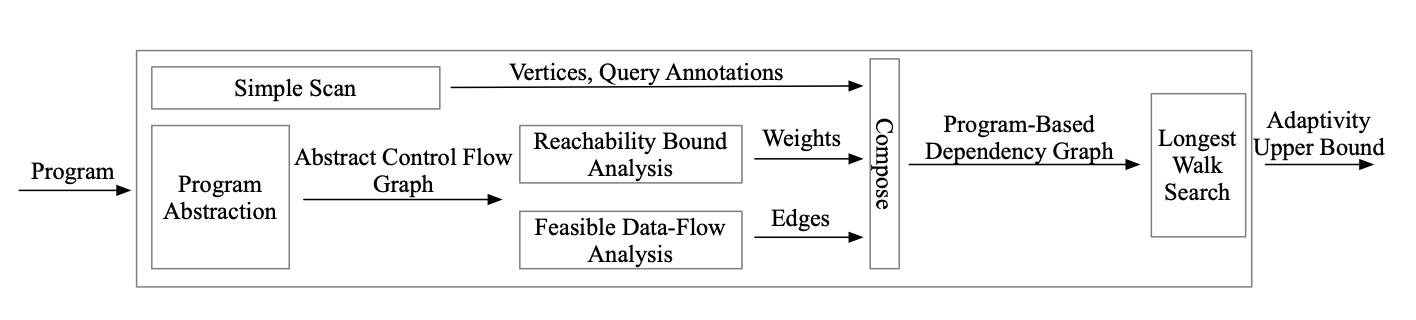
\includegraphics[width=1.0\columnwidth]{adapfun.png}
  \vspace{-0.3cm}
  \caption{The overview of {\THESYSTEM}}
  \label{fig:adaptfun}
  \vspace{-0.5cm}
\end{figure}
\subsubsection{Graph Estimation}
%
%
% \subsection{A guide to the algorithm}
% In order to have the upper bound of adaptivity:
% \\
% \begin{enumerate}
% \item $\THESYSTEM$  first builds a program-based dependency graph to {over-}approximate the
% % execution-based dependency graph (in Definition~\ref{def:trace_graph})
% Execution-Based Dependency Graph (in Definition~\ref{def:trace_graph})
% through Section~\ref{sec:alg_vertexgen}, Section~\ref{sec:alg_weightedgegen} and~\ref{sec:alg_graphgen}:
% % in the phases one to phases four of $\THESYSTEM$ in Section~\ref{sec:abscfg} to Section~\ref{sec:alg_graphgen}:
% \\
% 1.1 approximate the vertices: 
% % in the forth step of
% in the first phase of $\THESYSTEM$ in
% % the algorithm in Section~\ref{sec:alg_graphgen} 
% Section~\ref{sec:alg_vertexgen}
% without extra static analysis technique.
% \\
% 1.1 approximate the query annotations: 
% % in the forth step of
% in the first phase of $\THESYSTEM$ in
% % the algorithm in Section~\ref{sec:alg_graphgen} 
% Section~\ref{sec:alg_vertexgen}
% without extra static analysis technique.
% \\
% 1.2 approximate the vertices weights:
% in the second phase of 
% % the algorithm in  
% of $\THESYSTEM$ specifically in Section~\ref{sec:alg_weightgen}
% \\
% 1.3 approximate the edges between vertices:
% also in the second phase of $\THESYSTEM$ specifically in 
% % Section~\ref{sec:alg_weightgen}
% Section~\ref{sec:alg_edgegen}
% \\
% 1.4 generate the final approximated program-based dependency graph in Section~\ref{sec:alg_graphgen}
% %  to {over-}approximate the
% % approximate the query annotation: 
% % in the forth step of
% in the third phase of $\THESYSTEM$.
% % the algorithm  without extra static analysis technique.
% % \\
% This program-based graph has a similar topology structure as 
% % the one
% % of 
% the Execution-Based Dependency Graph. It has the same
% vertices and query annotations, but approximated edges and weights. 
% \item Then in the last phase in Section~\ref{sec:alg_adaptcompute}, $\THESYSTEM$
% % we compute the upper bound for adaptivity over this approximated graph:
% % , as an upper bound for
% % program's adaptivity
% computes the upper bound for adaptivity over this approximated graph.
% % in the last phase of this algorithm in Section~\ref{sec:alg_adaptcompute}.
% % \subsection{Adaptivity Based on Program Analysis in \THESYSTEM}
% % In order to give a bound on the program's adaptivity, we first build a
% % program-based data-dependency graph to {over-}approximate the
% % trace-based dependency graph.  Then, we define a program-based
% % adaptivity over this approximated graph, as an upper bound for
% % $A(c)$.
% \end{enumerate}
According to the dependency graph we use in adaptivity definition, we want to build a similar graph to {over-}approximate the
% execution-based dependency graph (in Definition~\ref{def:trace_graph})
Execution-Based Dependency Graph (in Definition~\ref{def:trace_graph}). The construction considers the vertices, edges, and the weight of every node, as well as some annotations which marks the query usage. The overall picture of this step is organized as follows.
% through Section~\ref{sec:alg_vertexgen}, Section~\ref{sec:alg_weightedgegen} and~\ref{sec:alg_graphgen}:


\begin{enumerate}
\item  Vertices are the assigned variables with unique labels, which is extracted directly from the program, see Section~\ref{sec:alg_vertexgen}
without extra static analysis technique
% \item Query annotations are also decided directly from the program, when there is a query request, the associated variables which are the results of the query requests are marked in the form of a flag, $0$ means no query, $1$ represents query related. See Section~\ref{sec:alg_vertexgen}.
\item The edge between vertices considers both control flow and data flow, See
Section~\ref{sec:alg_edgegen}
\item Every vertex and edge come with a weight, which tells the maximal times each vertex and edge can be visited in realistic execution. This weight is estimated by a reachability bound analysis on each vertex, See Section~\ref{sec:alg_weightgen}.
% \item Each edge also vertices considers both control flow and data flow, See
% Section~\ref{sec:alg_edgegen}
\item  Finally, with all the ingredients ready, we construct the final approximated program-based dependency graph in Section~\ref{sec:alg_graphgen}
\end{enumerate}

% the algorithm  without extra static analysis technique.
% \\
Overall, this program-based graph has a similar topology structure as 
% the one
% of 
the Execution-Based Dependency Graph. It has the same
vertices and query annotations, but approximated edges and weights. We call the graph generated by static analysis techniques, static analysis dedendency graph. 
% \item Then in the last phase in Section~\ref{sec:alg_adaptcompute}, $\THESYSTEM$
% % we compute the upper bound for adaptivity over this approximated graph:
% % , as an upper bound for
% % program's adaptivity
% computes the upper bound for adaptivity over this approximated graph.
% in the last phase of this algorithm in Section~\ref{sec:alg_adaptcompute}.
% \subsection{Adaptivity Based on Program Analysis in \THESYSTEM}
% In order to give a bound on the program's adaptivity, we first build a
% program-based data-dependency graph to {over-}approximate the
% trace-based dependency graph.  Then, we define a program-based
% adaptivity over this approximated graph, as an upper bound for
% $A(c)$.


\subsubsection{Adaptivity Computation}

Likewise the adaptivity is defined as a finite walk in the execution based depdenency graph, our static estimation on this adaptivity also relies on finding a path in the static analysis depdenency graph.   The construction of the stastic analysis dependency graph is of great value of showing some useful properties of the target program, such as dependency between variables, the execution upper bound of a certian command, while the key novelty is our path searching algorithm, which connects all the information we need in the static anlaysis dependency graph and provides us a sound over-estimation of adaptivity! In order to get a sound but precise upper bound, we will discuss some challenges in finding the 'appropriate' path in the graph, and how our algorithm responds to these challengs. We present the path seaching algorithm in Section~\ref{sec:alg_adaptcompute}.
 
% An
% approximated edge correspond to a program-based data dependency
% relation ($\flowsto$ in Definition~\ref{def:flowsto}) and an approximated
% weight corresponds to a reachability bound analysis results from
% Definition~\ref{def:transition_closure}.

% %
% \subsubsection{Program-Based Variable Dependency}
% The program-based dependency relation over two labeled variables ($x^i, y^j)$ is defined as a $\flowsto$ relation with respect to the program $c$ as follows.
% %
% \begin{defn}[Data Flow Relation between Assigned Variables ($\flowsto$)].
% \label{def:flowsto}
% \\
% Given a program  ${c}$,
% a variable ${x^i}  \in \lvar_c $ is in the \emph{flows to} relation with another variable ${y^j} \in \lvar_c$, if and only if:
% \mg{I cannot even parse the next formula. Why there is a big disjunction on the left? Disjunction is a binary operation, or n-ary if given a set, what is this disjunction between?}\\
% \mg{please, remove the underscript $c$ in the exists. It just makes everything mroe difficult to parse.}\\
% \mg{The use of $\lor$ is odd. E.g. $\exists {(\expr \lor \qexpr)}$ or
%   $ [{\assign{y}{\expr \lor \query(\qexpr)}}]^{j} $. I suggest to write the whole formula instead of using weird shortenings.}\\
% \mg{Also, now it is too late to change this but instead of breaking down the definition using the subterm relation and then defining the flowto relation, it would have been better to give just one inductive definition of Flowto - I imagine that this makes also the proof more awkward.}
% %
% {\footnotesize 
% \[
% \begin{array}{l}
% \flowsto({x^i, y^j, c}) \triangleq 
% \\
% \left( \bigvee
% \begin{array}{l}
% (\exists \expr \st \clabel{\assign{y}{\expr}}^j \in_{c} {c} 
% \land {x} \in FV(\expr) \land (x^i \in \live(j, c)))
% \\
% (\exists {\qexpr} \st [\assign{y}{\query({\qexpr})}]^j \in_{c} {c} 
% \land x \in FV({\qexpr}) \land (x^i \in \live(j,c))))
% \\
% \Big(\exists {c_w} \in \cdom, l \in \mathcal{L}, \bexpr \st
% 	\ewhile [\bexpr]^l \edo {c_w} \in_{c} {c}
% 	\land \flowsto(x^i, y^j, c_w)
% 	\\ \qquad	
%      \lor 
% 	\big( \exists {(\expr \lor \qexpr)} \st
% 	[{\assign{y}{\expr \lor \query(\qexpr)}}]^{j} \in_{c}  {c_w}  \land {x} \in FV(\bexpr) \land x^i \in \live(l, c)
% 	\big)
% 	\Big)
% \\
% \Big(
% \exists {c_1}, {c_2} \in \cdom, l \in \mathcal{L}, \bexpr 
% \st 
% 	\eif([\bexpr]^l, {c_1}, {c_2}) \in_{c} {c} \land
% 	\flowsto(x^i, y^j, c_1) \lor \flowsto(x^i, y^j, c_2)
% 	\\ \qquad 
% 	\lor 
% 	\big( \exists {(\expr \lor \qexpr)} \st
% 	\land {x} \in FV(\bexpr) \land x^i \in \live(l, c) \land
% 	([{\assign{y}{\expr \lor \query(\qexpr)}}]^{j} \in_{c}  {c_1}  
% 	\lor [{\assign{y}{\expr \lor \query(\qexpr)}}]^{j} \in_{c}  {c_2})
% 	\big)
% \Big)
% % \\
% \end{array}
% \right).
% \end{array}
% \]
% }
% %
% \end{defn}
% %
% \mg{The next notation is inconsistent with the one used above. Also, this definition should be given before the definition of flowto. From the description I have no cluse what this notion of reachability means. Also, the definition is referred to does not define this notation.}\\
% \mg{the definition somehow seems to make sense but until when the or notation is fixed and I don't see the definition of RD, I cannot tell for sure.}
% $\live^l(c) \subseteq \lvar_c$,
% which is the set of all the reachable variables at location of label $l$ in the program $c$.
% For every labelled variable $x^l$ in this set, 
% the value assigned to that variable
% in the assignment command associated to that label is reachable at the entry point of  executing the command of label $l$.
% This is formally defined , formally computed in Definition~\ref{def:feasible_flowsto}
% \\
% \mg{This description seems inconsistent with the definition. I suggest to use the same variables and terms.}
% To understand the $\flowsto$ intuition, 
% given a program  ${c}$ with its labelled variables $\lvar_c$, and two variables ${x^i}, y^j  \in \lvar_c $ 
% % showing up as $i$-th, $j$-th elements in $\lvar$ 
% % (i.e., ${x} = \lvar(i)$ and ${y} = \lvar(j)$),
% we say $y^j$ flows to ${x^i}$ in ${c}$ if and only if 
% the value of $y^j$ directly or indirectly influence the evaluation of the value of ${x}$ as follows:
% %
% \begin{itemize}
% \item (Explicit Influence) The program ${c}$ contains either 
% a command $[\assign{{x}}{\aexpr}]^i$ or $[\assign{{x}}{\query({\qexpr})}]^i$,
% such that ${y}$ shows up as a free variable in $\expr$ or ${\qexpr}$.
% We use $\flowsto({x^i, y^j, c})$ to denote $y^j$ flows to $x^i$ in ${c}$.
% %
% \item (Implicit Influence) The program ${c}$ contains either a while loop
% command
% or if command, 
% such that $x$ shows up in the guard
% and $y$ shows up in the left hand of an assignment command and this assignment command showing up
%  in the body of the while loop, or branches of if command.
% \end{itemize}
% %
% % This is formally defined in \ref{def:flowsto}.
% % We use $FV(\expr)$, $FV(\sbexpr)$ and $FV(\qexpr)$ denote the set of free variables in 
% % expression $\expr$, boolean expression $\sbexpr$ and query expression $\qexpr$ respectively.
% %
% %
% \mg{I don't understand what this definition of equivalence means. It is not observational equivalence
% and it is not syntactic equivalence. What are we trying to capture here? Also, it is equivalence of programs, not of program.}
% \begin{defn}[Equivalence of Program]
% %
% \label{def:aq_prog}
% Given 2 programs $c_1$ and $c_2$:
% \[
% c_1 =_{c} c_2
% \triangleq 
% \left\{
%   \begin{array}{ll} 
%     \etrue        
%     & c_1 = \eskip \land c_2 = \eskip
%     \\ 
%     \forall \trace \in \mathcal{T} \st \exists v \in \mathcal{VAL}
%     \st \config{ \trace, \expr_1} \aarrow v \land \config{ \trace, \expr_1} \aarrow v     
%     & c_1 = \assign{x}{\expr_1} \land c_2 = \assign{x}{\expr_2} 
%     \\ 
%     \qexpr_1 =_{q} \qexpr_2       
%     & c_1 = \assign{x}{\query(\qexpr_1)} \land c_1 = \assign{x}{\query(\qexpr_2)} 
%     \\
%     c_1^f =_{c} c_2^f \land c_1^t =_{c} c_2^t
%     & c_1 = \eif(b, c_1^t, c_1^f) \land c_2 = \eif(b, c_2^t, c_2^f)
%     \\ 
%     c_1' =_{c} c_2'         
%     & c_1 = \ewhile b \edo c_1' \land c_2 = \ewhile b \edo c_2'
%     \\ 
%     c_1^h =_{c} c_2^h \land c_1^t =_{c} c_2^t
%     & c_1 = c_1^h;c_1^t \land c_2 = c_2^h;c_2^t 
%   \end{array}
%   \right.
% \]
% %
% As usual, we denote by $c_1 \neq_{c} c_2$ the negation of the equivalence.
% %
% \end{defn}
% %
% \mg{This definition needs to go before it is used. }
% Given 2 programs $c$ and $c'$, we denote by $c' \in_{c} c$  that $c'$ is a sub-program of $c$ defined as follows,
% \begin{equation}
% c' \in_{c} c \triangleq \exists c_1, c_2, c''. ~ s.t.,~
% c =_{c} c_1; c''; c_2 \land c' =_{c} c''
% \end{equation} 
% %

% \subsubsection{Program Analysis Based Dependency Graph}
% We give the formal definition for the program-based dependency graph for a program $c$, 
% $\progG({c}) = (\vertxs, \edges, \weights, \flag)$ as follows.
% \begin{defn}
%     [Program-Based Dependency Graph].
%     \label{def:prog_graph}
%     \\
% Given a program ${c}$
% its program-based graph 
% $\progG({c}) = (\vertxs, \edges, \weights, \qflag)$ is defined as:
% {\footnotesize
% \[
% \begin{array}{rlcl}
% \text{Vertices} &
% \vertxs & := & \left\{ 
% x^l \in \mathcal{LV} 
% ~ \middle\vert ~
% x^l \in \lvar_{c}
% \right\}
% \\
% \text{Directed Edges} &
% \edges & := & 
% \left\{ 
%   ({x}_1^{i}, {x}_2^{j}) \in \mathcal{LV} \times \mathcal{LV}
%   ~ \middle\vert ~
%   \begin{array}{l}
%     {x}_1^{i}, {x}_2^{j} \in \vertxs
% 	\land
%     % \\
%     \exists n \in \mathbb{N}, z_1^{r_1}, \cdots, z_n^{r_n} \in \lvar_{{c}} \st 
%     n \geq 0 \land
%     \\
%     \flowsto(x^i,  z_1^{r_1}, c) 
%     \land \cdots \land \flowsto(z_n^{r_n}, y^j, c) 
%   \end{array}
% \right\}
% \\
% \text{Weights} &
% \weights & := &
% % \bigcup
% % \begin{array}{l}
% 	\left\{ (x^l, w) \in  \mathcal{LV} \times EXPR(\constdom)
% 	\mid
% 	x^l \in \lvar_{{c}} \land w = \absW(l)
% 	\right\}
% % \end{array} 
% \\
% \text{Query Annotation} &
% \qflag & := & 
% \left\{(x^l, n)  \in  \mathcal{LV} \times \{0, 1\} 
% ~ \middle\vert ~
%  x^l \in \lvar_{c},
% n = 1 \iff x^l \in \qvar_{c} \land n = 0 \iff  x^l \in \qvar_{c} .
% \right\}
% \end{array}
% \] 
% }
% , where the $\absW(l)$ is the symbolic reachability bound in domain of $EXPR(\constdom)$,
% % for the assignment command of label $l$ to which  
% the labeled variable $x^l$, 
% % is associated, 
% computed from the $\THESYSTEM$ algorithm 
% in Definition~\ref{def:transition_closure}.
% The $EXPR(\constdom)$ is an expression over symbolic constants containing the
% input variables and natural number.
% \end{defn} 
% %
% \paragraph{Program-Based Adaptivity ($\progA(c)$)}
% %
% Given a program ${c}$, we generate its program-based graph 
% $\progG({c}) = (\vertxs, \edges, \weights, \qflag)$.
% %
% Then the adaptivity bound based on program analysis for ${c}$ 
% % is the number of query vertices on a finite walk in $\progG({c})$. This finite walk satisfies:
% % \begin{itemize}
% % \item the number of query vertices on this walk is maximum
% % \item the visiting times of each vertex $v$ on this walk is bound by its reachability bound $\weights(v)$.
% % \end{itemize}
% is computed as the maximum query length over all finite walks in $\walks(\progG({c}))$,
% %
% % It is formally defined in \ref{def:prog_adapt}.
% defined formally as follows.
% %
% %
% \begin{defn}
% [{Program-Based Adaptivity}].
% \label{def:prog_adapt}
% \\
% {
% Given a program ${c}$ and its program-based graph 
% $\progG({c}) = (\vertxs, \edges, \weights, \qflag)$,
% %
% the program-based adaptivity for $c$ is defined as%
% \[
% \progA({c}) 
% := \max
% \left\{ \qlen(k)\ \mid \  k\in \walks(\progG({c}))\right \}.
% \]
% }
% \end{defn}  
%
%
% {
% \begin{defn}[Variable Flags ($\flag$)].
% \\
% Given a program  ${c}$ with its labelled variables $\lvar$, the $\flag$ is a vector of the same length as $\lvar$, s.t. for each variable ${x}$ showing up as the $i$-th element in $\lvar$ (i.e., ${x} = \lvar(i)$), 
% $\flag(i) \in \{0, 1, 2\}$ is defined as follows:
% %
% %
% \[
% \flag(i) := 
% \left\{
% \begin{array}{ll}
% 2 & 
% {x^l} \in \lvar_{c} \land 
% (\exists {\qexpr}. ~ s.t., ~
% [\assign{{x}}{\query({\qexpr})}]^l \in_{c} {c})
% \\
% 1 &  
% \begin{array}{l}
% {x^l} \in \lvar_{c} \bigwedge \\
% \left(
% \begin{array}{l}
% \big(\exists  ~ {c'}, {\expr}, \sbexpr, l, l'. ~
% 	\ewhile [\sbexpr]^l \edo {c'} \in_{c} {c}
% 	\land 
% 	[{\assign{x}{\expr}}]^{l'} \in_{c}  {c'}
% \big) \bigvee
% \\
% \big(\exists ~ \sbexpr, l, l_1, l_2, {c_1}, {c_2}, {\expr}_1, {\expr}_2. ~
% 	\eif([\sbexpr]^l, {c_1}, {c_2}) \in_{c} {c} \land
% 	([{\assign{x}{\expr_1}}]^{l1} \in_{c} {c_1} \lor 
% 	[{\assign{x}{\expr_2}}]^{l2} \in_{c} {c_2})
% \big)
% \end{array}
% \right)
% \end{array}
% \\
% 0 & \text{o.w.}
% \end{array}
% \right\}. 
% \] 
% %
% \end{defn}
%
% Operations on $\flag$ are defined as follows:
% \begin{equation}
% \begin{array}{llll}
% {\flag_1 \uplus \flag_2}(i) & := &
% \left\{
% \begin{array}{ll}
% k & k = \max{\big\{\flag_1(i), \flag_2(i)\big\}} 
% \land |\flag_1| = |\flag_2|\\
% 0 & o.w.
% \end{array}\right.
% & i = 1, \cdots, |\flag_1|  
% \\
% {\flag \uplus n}(i) & := & 
% \max\big\{ \flag(i), n \big\} 
% & i = 1, \ldots, |\flag|    
% \\
% \left[ n \right]^k (i) & := &  n
% & i = 1, \ldots, k ~ \land ~ |\left[ n \right]^k| = k
% \end{array}
% \end{equation}
%
%
%
% \begin{defn}[Data Flow Matrix ($\Mtrix$)]
% The data flow matrix $\Mtrix$ of a program $c$ is a matrix of size $|\lvar_c| \times |\lvar_c|$ 
% s.t.,
% %
% \[
% \Mtrix(i, j) \triangleq
% \left\{
% \begin{array}{ll}
% 1	&	\flowsto({x^i, y^j, c}) \\
% 0	& o.w.
% \end{array}
% \right., {x^i}, y^j  \in \lvar_c.
% \]
% %
% \end{defn}
% %
% Operations on the data flow matrices are defined as follows:
% %
% \begin{equation}
% \Mtrix_1 ; \Mtrix_2 
% := \Mtrix_2 \cdot \Mtrix_1 + \Mtrix_1 + \Mtrix_2
% \end{equation}
% %
% Consider the same program $c$ as above, its data flow matrix $\Mtrix$ and $\flag$ for the program $c$ is as follows:
% $$
% {c} = 
% \begin{array}{l}
% \left[{\assign {x_1} {\query(0)}}	\right]^1;
% \\
% \left[{\assign {x_2} {x_1 + 1}}		\right]^2;
% \\
% \left[{\assign {x_3} {x_2 + 2}}		\right]^3
% \end{array}
% ~~~~~~~~~~~~
% \Mtrix
% =  \left[ 
% \begin{matrix}
% 0 & 0 & 0 \\
% 1 & 0 & 0 \\
% 1 & 1 & 0 \\
% \end{matrix} \right] ~ , 
% \flag = \left [ \begin{matrix}
% 1 \\
% 0 \\
% 0 \\
% \end{matrix} \right ]
% $$
% %
% % There are two special matrices used for generating the data flow matrix $\Mtrix$ in the analysis algorithm. They are the left matrix $\lMtrix_i$ and right matrix $\mathsf{R_{(e, i)}}$.

% % Given a program  ${c}$ with its labelled variables $\lvar$ of length $N$,
% % the left matrix $\lMtrix_i$ generates a matrix of $1$ column, $N$ rows, 
% % where the $i$-th row is $1$ and all the other rows are $0$.
% % %
% % \begin{defn}[Left Matrix ($\lMtrix_i$)].
% % \\
% % Given a program  ${c}$ with its labelled variables $\lvar$ of size $N$, 
% % the left matrix $\lMtrix_i$ is defined as follows:
% % \[
% % \lMtrix_i(j) : = 
% % \left
% % \{
% % \begin{array}{ll}
% % 1 & j = i \\
% % 0 & o.w.
% % \end{array}
% % \right.,
% % j = 1, \ldots, N.
% % \]
% % \end{defn}
% % %
% % Given a program  ${c}$ with its labelled variables $\lvar$ of length $N$,
% % the right matrix $\rMtrix_{\expr, i}$ generates a matrix of one row and $N$ columns, 
% % where the locations of free variables in $\expr$ is marked as $1$. 
% % %
% % %
% % \begin{defn}[Right Matrix ($\rMtrix_{\expr}$)].
% % \\
% % Given a program  ${c}$ with its labelled variables $\lvar$ of length $N$, 
% % the right matrix $\rMtrix_{\expr}$ is defined as follows:
% % \[
% % \rMtrix_{\expr}(j) : = 
% % \left\{
% % \begin{array}{ll}
% % 1 & {x} \in FV(\expr) 
% % \\
% % 0 & o.w.
% % \end{array}
% % \right.,
% % {x} = \lvar(j) ~ , ~ j = 1, \ldots, N.
% % \]
% % %
% % %
% % \end{defn}
% % %
% % Using the same example program ${c}$ as above with labelled variables $\lvar = [ {x_1 , x_2 , x_3} ] $,
% % the left and right matrices w.r.t. its $2$-nd command 
% % $\left[{\assign {x_2} {x_1 + 1}}\right]^2$  are as follows:
% % \[
% % \lMtrix_1 = \left[ \begin{matrix}
% % 0   \\
% % 1 	 \\
% % 0   \\
% % \end{matrix}   \right ] 
% % ~~~~~~~~~~~~~~
% % \rMtrix_{{x}_1 + 1}
% % = \left[ \begin{matrix} 
% % 1 & 0 & 0 \\
% % \end{matrix}  \right]
% % \]
% %
% %
% %
% \subsection{ $\THESYSTEM$ Analysis Algorithm}
% \subsection{Dependency Graph Estimation}
\subsection{Vertices Estimationn}
\label{sec:alg_vertexgen}
The first component of every vertex in the static analysis dependency graph are actually identical as the  Execution-Based Dependency Graph, which are assigned variables in the program annotated with the unique label(line number). 
These vertices are collected by statically scanning the program, like what we do for vertices of its Execution-Based Dependency Graph. 
The vertices are defined formally as follows.

  \highlight{
\[
    \progV^0(c) \triangleq \left\{ 
  (x^l, w) \in \mathcal{LV} \times \mathcal{A}_{\lin}
  ~ \middle\vert ~
  x^l \in \lvar(c)
  \right\}
  \]
  }
  %
where $\mathcal{A}_{\lin}$ is the set of arithmetic expressions over $\mathbb{N}$ and program's input variables. 
The weight $w$ for every vertex will be computed in following step in Section~\ref{sec:alg_weightgen}.
% The static scanning of the programs also tells us whether one vertice(assigned variable) is assigned by a query request. We have similar definition when defining the Execution-Based Dependency Graph, 
% a set of pairs $\progF(c) \in \mathcal{P}(\mathcal{LV} \times \{0, 1\} )$ 
% % is the set of pairs 
% % The weight for each vertex in $\progV(c)$ is computed 
% mapping each $x^l \in \progV(c)$ to a flag, either $0$ or $1$, where $1$  means $x^{l}$ is a member of $ \qvar_{c}$, a set of those variables assigned with query requests, and $0$ means $x^{l}$ not in this set. It is defined formally below.

% \[\progF(c) =\left\{(x^l, n)  \in  \mathcal{LV} \times \{0, 1\} 
% ~ \middle\vert ~
% x^l \in \lvar_{c},
% n = 1 \iff x^l \in \qvar_{c} \land n = 0 \iff  x^l \not\in \qvar_{c} .
% \right\}\]
%

% \wq{To do: Add $\THESYSTEM$, a data flow analysis algorithm to scan the program and give a graph.}
% {\THESYSTEM} consists of three phases: 
% \begin{enumerate}
%     \item Generating an abstract control flow graph with each edge representing an abstract event transiting between two command labels. 
%     \item Computing the value bound invariant for each variable in the event and 
%     the event transition closure over the abstract control flow graph,
%     we get the reachability bound for each labeled command.
%     \item Refining the abstract control flow graph with data-flow, by performing the reaching definition analysis, we generate a weighted data control flow graph.
%     \item An algorithm to find the appropriate path in the weighted data control flow graph
% \end{enumerate}

% \begin{enumerate}
%     \item An algorithm to generate a precise data control flow graph
%     \item An algorithm to perform a Reachability number analysis to calculate the weight of each node in the graph generated in phase 1.
%     \item An algorithm to find the appropriate path in the weighted data control flow graph
% \end{enumerate}

\subsection{Edge and Weight Estimation}
\label{sec:alg_weightedgegen}

Since the edges of the execution-based graph of a program relies on the dependency relation, which handles both control flow and data flow, as an over-approximation of this graph, the edges of our static anlaysis dependency graph also covers these two kind of flows. We develop a feasible data flow relation to catch these two flows, in Section~\ref{sec:alg_edgegen}.


The weight of every vertice in the execution-based graph is built on all possible execution traces.
In order to over-approximate the weight statically but still tightly, we present a symbolic reachability bound analysis for estimation of the weight of each vertice(label) in Section~\ref{sec:alg_weightgen},
in spirit of some reachablility bound techiniques.


The edges and weight estimation are both performed on basis of an abstract control flow graph of the program, we first show how to generate this abstract execution control flow graph before the introduction of  the edge and weight estimation.  

% This analysis first 
%  generate an abstract control flow graph
%  over all program labels, 
% in order to analyzing the data flow relations through variables assigned in every labeled command,
% and the reaching time of each variable.
% Then, it refines this control flow graph 
% % into a weighted data-dependency graph, 
% and generate the Program-Based Dependency Graph,
% through the data flow and reaching bound analysis results.
% In the last step, it finds the longest finite walk in this weighted data control flow graph w.r.t. the query variables,
% and return the number of query vertices traversed alongside.
% % \wq{To do: Add $\THESYSTEM$, a data flow analysis algorithm to scan the program and give a graph.}
% To be more specific, {\THESYSTEM} consists of five phases as follows,
% \\
% % \jl{Better to have a graph or picture of overview of the algorithm}
% \todo{graph}
% \todo{pass again}
% This analysis
% \begin{enumerate}
%     % \item Generating 
%     \item first generate 
%     an abstract control flow graph
%     %  over all labels,
%     (remove?? with program's labels as vertices and abstract transitions as edges)
%     in Section~\ref{sec:abscfg},
%     % used to analyze 
%     for analyzing the weight of every vertex in $\progV(c)$ and edges between every vertex in $\progV(c)$ in the next two steps;
%     %  \ref{sec:alg_weightgen} and 
%     % \ref{sec:alg_edgegen}.

%     % which are used as program's control locations,
%     %
%     \item then use the abstract control flow graph generated above, 
%     compute the weight of every vertex in $\progV(c)$ by computing a symbolic reachability bound for each label in Section~\ref{sec:alg_weightgen},
%     % \\
%     \item and then use the same graph again to estimate the edges between every vertex in $\progV(c)$ by computing the feasible data flow relation between every labeled variables in Section~\ref{sec:alg_edgegen}.
  
% \end{enumerate}

\subsubsection{Abstract Execution Control Flow graph}
\label{sec:abscfg}
% In an 
%  % a program $c$ 
%  abstract control flow graph for a program $c$, $\absG(c)$, 
%  every 
%  vertex corresponds to the unique
%  label.
%  Specifically,
%  The edge is directed, 
%   representing an abstract transition 
%   between two control locations uniquely decided by the labels.   
%    (We refer control location and the label to the same thing). The abstract transition is of the form of a set of difference constraints for variables, built from the abstract execution trace of the program. For instance, the edge $(l_1, dc, l_2)$ from $l_1$ to $l_2$,
%   represents an abstract transition 
%   between two control locations with a set of difference constraints on it.
%  In this transition, the  command labeled with the second location $l_2$, 
%   will be executed after execution of the command with label $l_1$,
%  %  The abstract transition contains a set of difference constraints for variables, 
%  with the difference constraints generated by abstracting the command of the first label. Difference constraints is a constraint on difference between variables and constants, which will be formally introduced when we discuss experssion abstraction.
%  \wq{The edge in the abstract control flow graph comes from the abstract execution trace of the program. The abstract execution trace, an abstract representation of the execution, consists of a list of abstract transitions. Then, every abstract transition in the abstrction execution trace corresponds to an edge in the abstract control flow graph. In aonther word, the edge $(l_1, dc, l_2)$ in the abstract control flow graph, represents an abstract transition 
%   from $l_1$ to $l_2$, with a set of difference constraints $dc$. Also notice, the difference constraints generated during the abstract transition appears in the edge as annotation.}

%  % over program's abstract execution 

%  Overall, the key point of the abstract excution control flow graph is the construction of the abstract execution trace of a program, which relies on a program abstraction procedure in following steps:

%  \begin{enumerate}
%  \item  Computing the abstract expression for every assignment command in the program.
%  \item Computing the abstract event for every labeled command in the program. Intuitively, this abstract event aims 
%  to approximate the event in program's execution trace.
%  \item Constructing the abstract execution trace for a program.
%  \end{enumerate}  

We discuss the vertices and edge of the
abstract control flow graph for a program $c$, $\absG(c)$.

Every 
vertex corresponds to the unique
label.
Specifically,
the vertices of this graph is the set of $c$'s labels with an exit label $l_{ex}$, 
\[ 
  \absV(c) = labels(c)\cup\{l_{ex}\}
  \]
%  corresponding to a label command in the program.

% \wq{
  The edge in the abstract control flow graph comes from the abstract execution trace of the program. 
  The abstract execution trace, an abstract representation of the execution, consists of a list of abstract transitions. 
  Then, every abstract transition in the abstraction execution trace corresponds to an edge in the abstract control flow graph. In another word, the edge $(l_1, dc, l_2)$ in the abstract control flow graph, represents an abstract transition 
 from $l_1$ to $l_2$, with a set of difference constraints $dc$. 
 Also notice, the difference constraints generated during the abstract transition appears in the edge as annotation.
%  }

% over program's abstract execution 


% \wq{
  Overall, the vertices can be easily collected and the key point of construction of the abstract execution control flow graph for a program is the abstract execution trace, 
  which relies on the abstraction of expression and abstract transition (we also call it abstract event), we will discuss in the following section.
   To make it easy to understand, abstract control flow graph is a control flow graph, with difference constraints on every edge.
  % }  

%
\paragraph*{Expression Abstraction}

The expression assigned to the variable on the left hand of the assignment command is abstracted to an abstract value: (adopted from the expression abstraction method in paper \cite{sinn2017complexity}). The abstract value is expressed in the form of Difference constraint, denotated as $DC : \mathcal{VAR} \cup \constdom \to \mathcal{\mathcal{VAR} \times (\mathcal{VAR} \cup \constdom) } \times (\mathbb{Z} \cup \{\infty\})$.  $\constdom$ is called the Symbolic Constant defined as $\constdom \triangleq \mathbb{N} \cup \inpvar \cup \{\max{(\dbdom)}\} $, which consists of 
natural numbers $\mathbb{N}$,
the program's input variables $\inpvar$  
and a constant value $Q_m$ for estimating the upper bound of variables which are
assigned by queries. 

Give an instance of difference constraint used here,
$DC(\mathcal{VAR}  \cup \constdom) \cup \{\top\}$ represents all the difference constraints over 
variable and symbolic constants. 
% The difference constraint $DC$ over $\mathcal{VAR} \cup \constdom$ 
It is a set of the inequality of form $x \leq y + v$ where $x \in \mathcal{VAR} $, 
$y \in \mathcal{VAR}  \cup \constdom$ and $v \in \mathbb{Z}$. 
This difference constraint is defined in the same way as
\cite{sinn2017complexity}. For concise, we use $\dcdom^{\top}$ to represent the $DC(\mathcal{VAR}  \cup \constdom) \cup \{\top\}$ .


We show the expression abstraction $\absexpr : \expr \to \mathcal{VAR} \to DC(\mathcal{VAR}  \cup \constdom) \cup \{\top\} $ below.

% We introduce the following notations and operations first
% % an expression abstraction method based on the expression abstraction in paper \cite{sinn2017complexity}.
% \\
% % is enriched into $\constdom \triangleq \mathbb{N} \cup \inpvar \cup \{\max{(\dbdom)}\} $.
% T
% \\

% represents the set of inequality over all $\mathcal{VAR}  \cup \constdom$. 

% The symbolic constant is enriched into $\constdom \triangleq \mathbb{N} \cup \inpvar \cup \{\max{(\dbdom)}\} $.
% It consists of 
% natural number $\mathbb{N}$,
% the symbolic constants $\inpvar$ (i.e., the set of the program's input variables), 
% and a constant value $Q_m$ for estimating the upper bound of variables which are
% assigned by queries.
% \\
% The symbolic constant is enriched into $\constdom \triangleq \mathbb{N} \cup \inpvar \cup \{\max{(\dbdom)}\} $.
% \\

% % $ \absdom: \mathcal{P}(DC(\mathcal{VAR}  \cup \constdom) \cup \{\top \})$:
% \\
% $\constdom: \mathbb{N} \cup \inpvar \cup \{\max{(\dbdom)}\} $ 
% The  constant 
% \\
% % $DC(\mathcal{VAR}  \cup \constdom)$ represents the set of inequality over all $\mathcal{VAR}  \cup \constdom$.
% \\

% \[
%   \begin{array}{ll} 
%     \absexpr(y + c, x)  = x' \leq y + c  & c \in \mathbb{N} \land y \in (VAR \cup \constdom) \\
%     \absexpr(y - c, x)  = x' \leq y - c  & c \in \mathbb{N} \land y \in (VAR \cup \constdom) \\
%     \absexpr(v, x)  = x' \leq v + 0  & v \in (VAR \cup \constdom) \\
%     \absexpr(\aexpr, x) = x' \leq 0 + \infty   & \aexpr \text{ doesn't have any of the forms as above} \\
%     \absexpr(\qexpr, x)  = x' \leq 0 + Q_m & \qexpr \text{ is a query expression}  \\
%     \absexpr(\bexpr, x) = x' \leq 0 + 1   & \bexpr \text{ is a boolean expression} \\
%   \end{array}
%   \]
  \[
    \begin{array}{ll} 
      \absexpr(x - v, x)  = x' \leq x - v  & x \in \grdvar \land v \in \mathbb{N} \\
      \absexpr(y + v, x)  = x' \leq y + v  & x \in \grdvar \land v \in \mathbb{Z} \land y \in (\grdvar \cup \constdom) \\
      \absexpr(v, x)  = x' \leq v + 0  & x \in \grdvar \land v \in (\grdvar \cup \constdom) \\
      \absexpr(y + v, x)  = x' \leq y + v & \\
      \grdvar = \grdvar \cup \{y\} & x \in \grdvar \land v \in \mathbb{Z} \land y \notin (\grdvar \cup \constdom)  \\
      \absexpr(\qexpr, x)  = x' \leq 0 + Q_m & x \in \grdvar \land \qexpr \text{ is a query expression}  \\
      \absexpr(\bexpr, x) = x' \leq 0 + 1   & x \in \grdvar \land \bexpr \text{ is a boolean expression} \\
      \absexpr(\expr, x) = x' \leq \infty  &  x \in \grdvar \land \expr \text{ doesn't have any of the forms as above} \\
      \absexpr(\expr, x) = \top  &  x \notin \grdvar \\
    \end{array}
    \]
  
  % \wq{ 
    $\grdvar$ is the set of variables used in the guard expression of every while command in the program $c$. 
  % }. 
  In the case 4, if a variable $x$, belonging to the set 
  $\grdvar$ is updated by a variable $y$, which isn't in this set, 
  we add $y$ into the set $\grdvar$ and repeat 
  above procedure  until $\grdvar$ and $\absexpr(\expr, x)$ is stabilized. 
  % \wq{I do not understand this sentence:-(}
  \\
Specifically 
% understanding the intuition, 
we handle a 
% simplified 
normalized guard expression ($ x > 0$ for $x^l \in \lvar_c$)
 in $\ewhile$, and 
%  \wq{I do not understand this sentence:-(}
%  .
% \\
% The counter variables only increase, decrease or reset by expression in the form of arithmetic minus and plus (able to extend to max and min.)
the counter variables only increase, decrease or reset by 
% expression in the form of 
simple arithmetic expression (mainly multiplication, division, minus and plus (able to extend to max and min)). 
This is the same as in paper \cite{sinn2017complexity}. 
\\
For more complex expression assignments, where the counter reset, or calculated from $\elog$, 
multiplication or division, and expressions involving multiple variables, the constraint is approximated as reset of $\infty$.
\\
% This simplification \wq{which part we simplify here?} 
This approximation strategy
doesn't affect our analysis results in our examples. It is easy to extend the normalized expression 
into more complex forms as in \cite{sinn2017complexity}, as well as the 
counter variable manipulation with more advanced expressions.
% \\ 
% The boolean expression in the guard of $\ewhile$ command is normalized into form of $ x > 0$ where $x^l \in \lvar_c$ for some $l$.


\paragraph{Program Event Abstraction}
We show the abstract event definition, which is generated when computing its abstract execution trace.

\begin{defn}[Abstract Event]
  \label{def:abs_event}
  Abstract Event: 
  $\absevent \in $
  $\ldom \times \dcdom^{\top} \times \ldom$
  is a 
  % pair of abstract initial state and final state.
  triple where the first and third components are labels,
  second component is a constraint from $\dcdom^{\top}$.
  % the thrid % computed from program's abstract final and initial state, $\absfinal(c)$ and $\absinit(c)$ with formal definition, and algorithm detail in Appendix.
  %  the constraint and the third corresponds to a final state.
  \end{defn}
  Specifically, in an abstract event, 
  the first label correspond to an initial state, and 
  the second label and the constraint correspond to an abstract final state.
 The abstract initial state is a label from $\ldom$.
The abstract final state is a pair from $\ldom \times \dcdom^{\top}$,  
where first component is a label from $\ldom$ and the second component is a constraint from $\dcdom^{\top}$.
%

%
Given a program $c$, its abstract initial state,
and the set of its abstract final state is computed as follows,
%
\[
  \begin{array}{ll}
    \absinit(\clabel{\assign{x}{\expr}}{}^l)  & = l  \\
    \absinit(\clabel{\assign{x}{\expr}}{}^l)  & = l \\
    \absinit(\clabel{\eskip}^{l})  & = l \\
    \absinit(\eif [b]^l \ethen c_1 \eelse c_2)  & = l \\
    \absinit(\ewhile [b]^l \edo c)  & = l \\
    \absinit(c_1 ; c_2)  & = \absinit(c_1) \\
 \end{array}
 \]
%
Final State Abstraction: 
$\absfinal: \cdom \to \mathcal{P}(\ldom \times \dcdom^{\top})$,
computes the set of Abstract Final State for the command. 
 \[
  \begin{array}{ll}
    \absfinal(\clabel{\assign{x}{\expr}}{}^l)  & = \{(l, \absexpr\eapp (\expr, x))\}  \\
     \absfinal(\clabel{\assign{x}{\query(\qexpr)}}{}^l)  & = \{
      (l, x' \leq 0 + Q_m )\}  \\
     \absfinal(\clabel{\eskip}^{l})  
     & = \{(l, \top)\} \\
     \absfinal(\eif [b]^l \ethen c_1 \eelse c_2)  & = \absfinal(c_1) \cup \absfinal(c_2) \\
     \absfinal(\ewhile [b]^l \edo c)  & = \{(l, \top)\} \\
     \absfinal(c_1 ; c_2)  & =  \absfinal(c_2) \\
 \end{array}
 \]
 %
 \paragraph{Abstract Execution Trace}
 Now, we  extract the abstract execution trace  $\absflow(c)$ for a program, which computes the Abstract Execution Trace for program $c$, as a set of the abstract events $\absevent$.
 %
 \begin{defn}[Abstract Execution Trace]
 \label{def:abs_trace}
  $\absflow \in \cdom \to \mathcal{P}( \ldom \times DC(\mathcal{VAR}  \cup \constdom) \cup \{\top\}) \times \ldom )$
  \end{defn}
 %

 
  We now show how to compute the abstract execution trace. 
  For simplicity, we use $\mathcal{P}(\absevent)$ represent the power set of all abstract events, and we have $\absflow(c) \in \mathcal{P}(\absevent)$.
 We first append a skip command with 
%  a symbolic label $l_e$, i.e., $\clabel{\eskip}^{l_e}$ at the end of the program $c$, and compute the $\absflow(c) = \absflow'(c')$ for $c'$, where $c' = c;\clabel{\eskip}^{l_e}$ as follows,
the exist label $l_{ex}$, i.e., $\clabel{\eskip}^{l_{ex}}$ at the end of the program $c$, 
and compute the $\absflow(c) = \absflow'(c')$ for $c'$, where $c' = c;\clabel{\eskip}^{l_{ex}}$ as follows,
 %
 {\footnotesize
 \[
   \begin{array}{ll}
      \absflow'(\clabel{\assign{x}{\expr}}{}^l)  & = \emptyset  \\
      \absflow'(\clabel{\assign{x}{\query(\qexpr)}}{}^l)  & = \emptyset  \\
      \absflow'([\eskip]^{l})  & = \emptyset \\
      \absflow'(\eif [b]^l \ethen c_t \eelse c_f)  & =  \absflow'(c_t) \cup \absflow'(c_f)
      %   \\ & \quad 
        \cup \{(l, \top,  \absinit(c_t) ) ,  (l, \top, \absinit(c_f)) \} \\
       \absflow'(\ewhile [b]^l \edo c_w)  & =  \absflow'(c_w) \cup \{(l, \top, \absinit(c_w)) \} 
      %  \\ & \quad 
       \cup \{(l', dc, l)| (l', dc) \in \absfinal(c_w) \} \\
       \absflow'(c_1 ; c_2)  & = \absflow'(c_1) \cup  \absflow'(c_2) 
      %  \\ & \quad 
       \cup \{ (l, dc, \absinit(c_2)) | (l, dc) \in \absfinal(c_1) \} \\
   \end{array}
   \]
   }

   Notice $\absflow'([x := \expr]^{l})$, $\absflow'([x := \query(\qexpr)]^{l})$ and $\absflow'([\eskip]^{l})$ are all empty set. 
   For every event $\event$ with label $l$ in an execution trace $\trace$ of program $c$, 
   there is an abstract event in program's abstract execution trace of form $(l, \_, \_)$.  
   We also show the soundness of the abstract execution trace in Appendix.
  %  which says 
  %  \wq{...}
   \begin{lem}[Soundness of the Abstract Execution Trace]
     \label{lem:abscfg_sound}
   Given a program ${c}$, we have:
   %
   \[
     \begin{array}{l}
       \forall \vtrace_0, \trace \in \mathcal{T} ,  \event = (\_, l, \_) \in \eventset \st
   \config{{c}, \trace_0} \to^{*} \config{\eskip, \trace_0 \tracecat \vtrace} 
   \land \event \in \trace 
   \\
   \qquad \implies \exists \absevent = (l, \_, \_) \in (\ldom\times \dcdom^{\top} \times \ldom) \st 
   \absevent \in \absflow(c)
   \end{array}
   \]
   \end{lem}
%    This lemma is proved formally in Appendix~\ref{apdx:reachability_soundness}.
% For every event $\event$ with label $l$ in an execution trace $\trace$ of program $c$, 
% there is an abstract event in program's abstract execution trace of form $(l, \_, \_)$. 
This lemma is proved formally in Lemma~\ref{lem:abscfg_sound} in Appendix~\ref{apdx:reachability_soundness}.
\\
For every labeled variable in program $c$, $x^l \in \lvar_c$, there is a unique abstract event in program's abstract execution trace $\absevent \in \absflow(c)$ of form $(l, \_, \_)$. 
\begin{lem}[Uniqueness of the Abstract Execution Trace]
  \label{lem:abscfg_unique}
Given a program ${c}$, we have:
%
\[
  \begin{array}{l}
    \forall \vtrace_0, \trace \in \mathcal{T} ,  \event = (\_, l, \_, \_) \in \eventset^{\asn} \st
\config{{c}, \trace_0} \to^{*} \config{\eskip, \trace_0 \tracecat \vtrace} 
\land \event \in \trace 
\\
\qquad \implies \exists! \absevent = (l, \_, \_) \in (\ldom\times \dcdom^{\top} \times \ldom) \st 
\absevent \in \absflow(c)
\end{array}
\]
\end{lem}
This lemma and proof is also 
formalized in Lemma~\ref{lem:absevent_unique} in Appendix~\ref{apdx:reachability_soundness}.

Then, we build the edge for $c$'s abstract control flow graph as follos,
\[
  \absE(c) = \{(l_1, dc, l_2) | (l_1, dc, l_2) \in \absflow(c)\}
  \]

% We have a pre-processing algorithm to go through the programs and returns the list of labels associating with a loop and whose visiting times need to be analyzed.
%


\paragraph{Abstract Control Flow Graph} 
With the vertices $\absV(c)$ and edges $\absE(c)$ ready, we construct the abstract control flow graph, formally 
% Through a program $c$'s abstract execution trace, its abstract control flow graph is computed 
defined in 
Definition~\ref{def:abs_cfg}.
% Given program $c$ with its abstract control flow $\absflow(c)$, the Abstract Control Flow Graph:
% \\
\begin{defn}[Abstract Control Flow Graph]
\label{def:abs_cfg}
Given a program $c$, 
with its abstract control flow $\absflow(c)$
its abstract control flow graph $\absG(c) =(\absV(c), \absE(c), \absW(c))$ is defined as follows,
\\
% \highlight{
% :
%
% \\
$\absE(c) = \{(l_1, dc, l_2) | (l_1, dc, l_2) \in \absflow(c)\}$,
\\
$\absV(c) = labels(c)\cup\{l_{ex}\}$
\\
 $\absW(c) 
\triangleq \left\{ (l, w) \in \mathbb{L} \times EXPR(\constdom) \right\}$.
% }
% \\
% , where the weight of every label to be computed in the next step.
\end{defn}
% 
% The vertices $\absV(c)$ in this graph are program's labels with an exit label $l_{ex}$.
% Each directed 
%  edge $(l_1, dc, l_2)$ from $l_1$ to $l_2$,
%  represents an abstract transition 
%  between two control locations with a set of difference constraints on it.
% %  , i.e., the labels of two commands (we call the labels also control location and they refer to the same thing), 
% %  where 
% In this transition, the  command labeled with the second location $l_2$, 
%  will be executed after execution of the command with label $l_1$,
% %  The abstract transition contains a set of difference constraints for variables, 
% with the difference constraints generated by abstracting the command of the first label.
% % \\
% % It is easy to show for every $(l_1, dc, l_2) \in \absflow(c)$ such that $l_2 \neq l_e$, $(l_1, l_2) \in flow(c)$. The formal Lemma and proof can be found in Lemma~\ref{lem:flow_to_absflow} in Appendix~\ref{apdx:reachability_soundness}.
Notice we also define the $\absW(c)$ in this graph without giving an actual value.
This $\absW(c)$ is the set of weight for every 
% vertex 
label. The weight is a symbolic expression over the symbolic constant, 
which is the estimated upper bound on the number of visiting time for every control location
through the reachability bound analysis as follows.
%
% It is easy to show for every $(l_1, dc, l_2) \in \absflow(c)$ such that $l_2 \neq l_e$, $(l_1, l_2) \in flow(c)$. The formal Lemma and proof can be found in Lemma~\ref{lem:flow_to_absflow} in Appendix~\ref{apdx:reachability_soundness}.
%
\paragraph*{Example}
% Look at the two-round example again, its generated abstract control is shown as in Figure~\ref{fig:adapfun_tworound}(a).
% In this abstract control flow graph, every vertex is a label,
% corresponding to a label command in the program.
% Each directed 
% edge represents an abstract transition 
% between two control locations, 
% i.e., the labels of two commands (we call the labels also control location and they refer to the same thing), 
% where the second labeled command will be executed after execution of the command with first label.
% For example, the edge $0, a \leq 0, 1$ on the top, represents,
% from location $0$, the command 
% $\clabel{\assign{a}{0}}^0$ is executed with next continuation location $1$,
% where the 
% command $\clabel{\assign{j}{k}}^1$ will be executed next.
% The constraint $a \leq 0$ is generated by abstracting from the assignment command $\assign{a}{0}$,
% representing that value of $a$ is less than or equals to $0$ after 
% location $0$ before executing command at line $1$.
% %
% The same way for the rest edges' constructions.
%
Let us look at the two-round example, its generated abstract control flow graph is shown as in Figure~\ref{fig:abscfg_tworound}(b).
For example, the edge $(0, a \leq 0, 1)$ on the top, tells us the command 
$\clabel{\assign{a}{0}}^0$ is executed with next continuation location $1$,
where the 
command $\clabel{\assign{j}{k}}^1$ will be executed next.
The constraint $a \leq 0$ is a difference constraint, generated by abstracting from the assignment command $\assign{a}{0}$,
representing that value of $a$ is less than or equals to $0$ after 
location $0$ before executing command at line $1$. The difference constraint is an inequality relation between, the left-hand side of the inequality talks about the variable before the execution and the right-hand side ascribes those after the execution. 
Look at the $a < a+x $ on the edge $5$ to $2$, which describes the execution of the command at line $5$, which is an assignment $a = a+x$. The $a$ on the left side of $a < a+x$ represents the value of $a$ after the assignment, while the right-hand side $a$ stores the value before the assignment. 
Also, we have while loop, which is a circle $2 \to 4 \to 5 \to 2$ in Figure~\ref{fig:abscfg_tworound}(b). 
Please also look at the edge from $3$ to $4$, which talks about the query! The $x < Q_m$ describes the execution of a query request (the command at line 3), the query results stored in $x$ is bounded by $Q_m$. 
$Q_m$ is the maximal value for query requesting result from the database $DB$. $top$ means there is no assignment executed, for example, we have the difference constraint $\top$ on the edge $2$ to $6$, means at line $2$, there is no assignment (it is a testing guard $j>0$.) 
%
The same way for the rest edges' constructions.
\begin{figure} 
  \centering
  \begin{subfigure}{.2\textwidth}
  \begin{centering}
  {\small
  $
      \begin{array}{l}
            \clabel{ \assign{a}{0}}^{0} ;   
              \clabel{\assign{j}{k} }^{1} ; \\
              \ewhile ~ \clabel{j > 0}^{2} ~ \edo ~ \\
              \Big(
               \clabel{\assign{x}{\query(\chi[j])} }^{3}  ; \\
               \clabel{\assign{j}{j-1}}^{4} ;\\
              \clabel{\assign{a}{x + a}}^{5}       \Big);\\
              \clabel{\assign{l}{\query(\chi[k]*a)} }^{6}\\
          \end{array}
  $
  }
  \caption{}
  \end{centering}
  \end{subfigure}
    \begin{subfigure}{.35\textwidth}
    \begin{centering}
  %   \todo{abstract-cfg for two round}
  \begin{tikzpicture}[scale=\textwidth/20cm,samples=200]
  \draw[] (-7, 10) circle (0pt) node{{ $0$}};
  \draw[] (0, 10) circle (0pt) node{{ $1$}};
  \draw[] (0, 7) circle (0pt) node{\textbf{$2$}};
  \draw[] (0, 4) circle (0pt) node{{ $3$}};
  \draw[] (0, 1) circle (0pt) node{{ $4$}};
  \draw[] (-7, 1) circle (0pt) node{{ $5$}};
  % Counter Variables
  \draw[] (6, 7) circle (0pt) node {\textbf{$6$}};
  \draw[] (6, 4) circle (0pt) node {{ $ex$}};
  %
  % Control Flow Edges:
  \draw[ thick, -latex] (-6, 10)  -- node [above] {$a \leq 0$}(-0.5, 10);
  \draw[ thick, -latex] (0, 9.5)  -- node [left] {$j \leq k$} (0, 7.5) ;
  \draw[ thick, -latex] (0, 6.5)  -- node [left] {$\top$}  (0, 4.5);
  \draw[ thick, -latex] (0, 3.5)  -- node [right] {$x \leq Q_m$} (0, 1.5) ;
  \draw[ thick, -latex] (-0.5, 1)  -- node [above] {$j \leq j - 1$} (-6, 1) ;
  \draw[ thick, -latex] (-6, 1.5)  -- node [left] {$a \leq a + x$} (-0.5, 7)  ;
  \draw[ thick, -latex] (0.5, 7)  -- node [above] {$l \leq Q_m$}  (5.5, 7);
  \draw[ thick, -latex] (6, 6.5)  -- node [right] {$\top$} (6, 4.5) ;
  \end{tikzpicture}
  \caption{}
    \end{centering}
    \end{subfigure}
    \begin{subfigure}{.35\textwidth}
      \begin{centering}
    %   \todo{abstract-cfg for two round}
    \begin{tikzpicture}[scale=\textwidth/20cm,samples=200]
    \draw[] (-10, 10) circle (0pt) node{{ $0: 1$}};
    \draw[] (0, 10) circle (0pt) node{{ $1: 1$}};
    \draw[] (0, 7) circle (0pt) node{\textbf{$2: k$}};
    \draw[] (0, 4) circle (0pt) node{{ $3: k$}};
    \draw[] (0, 1) circle (0pt) node{{ $4: k$}};
    \draw[] (-10, 1) circle (0pt) node{{ $5: k$}};
    % Counter Variables
    \draw[] (6, 7) circle (0pt) node {\textbf{$6: 1$}};
    \draw[] (6, 4) circle (0pt) node {{ $ex: 1$}};
    %
    % Control Flow Edges:
  \draw[ thick, -latex] (-8, 10)  -- node [above] {$a \leq 0$}(-1.5, 10);
  \draw[ thick, -latex] (0, 9.5)  -- node [left] {$j \leq k$} (0, 7.5) ;
  \draw[ thick, -latex] (0, 6.5)  -- node [left] {$\top$}  (0, 4.5);
  \draw[ thick, -latex] (0, 3.5)  -- node [right] {$x \leq Q_m$} (0, 1.5) ;
  \draw[ thick, -latex] (-1.5, 1)  -- node [above] {$j \leq j - 1$} (-8, 1) ;
  \draw[ thick, -latex] (-8, 1.5)  -- node [left] {$a \leq a + x$} (-1.5, 7)  ;
  \draw[ thick, -latex] (1.5, 7)  -- node [above] {$l \leq Q_m$}  (4.5, 7);
  \draw[ thick, -latex] (6, 6.5)  -- node [right] {$\top$} (6, 4.5) ;
    \end{tikzpicture}
    \caption{}
      \end{centering}
      \end{subfigure}
  %       \begin{subfigure}{.3\textwidth}
  %   \begin{centering}
  %   \begin{tikzpicture}[scale=\textwidth/18cm,samples=200]
  % \draw[] (0, 10) circle (0pt) node
  % {{ $a^0: {}^1_{0}$}};
  % \draw[] (0, 7) circle (0pt) node
  % {\textbf{$x^3: {}^{k}_{1}$}};
  % \draw[] (0, 4) circle (0pt) node
  % {{ $a^5: {}^{k}_{0}$}};
  % \draw[] (0, 1) circle (0pt) node
  % {{ $l^6: {}^{1}_{1}$}};
  % % Counter Variables
  % \draw[] (5, 9) circle (0pt) node {\textbf{$j^2: {}^{1}_{0}$}};
  % \draw[] (5, 6) circle (0pt) node {{ $j^4: {}^{k}_{0}$}};
  % %
  % % Value Dependency Edges:
  % \draw[ ultra thick, -latex, densely dotted,] (0, 1.5)  -- (0, 3.5) ;
  % \draw[ ultra thick, -latex, densely dotted,] (0, 4.5)  -- (0, 6.5) ;
  % \draw[ thick, -latex] (0, 7.5)  -- (0, 9.5) ;
  % \draw[ thick, -Straight Barb] (1.5, 3.5) arc (120:-200:1);
  % \draw[ thick, -Straight Barb] (6.5, 6.5) arc (150:-150:1);
  % \draw[ thick, -latex] (5, 6.5)  -- (5, 8.5) ;
  % % Control Dependency
  % \draw[ thick,-latex] (1.5, 7)  -- (4, 9) ;
  % \draw[ thick,-latex] (1.5, 4)  -- (4, 9) ;
  % \draw[ thick,-latex] (1.5, 7)  -- (4, 6) ;
  % \draw[ thick,-latex] (1.5, 4)  -- (4, 6) ;
  % \end{tikzpicture}
  % \caption{}
  %   \end{centering}
  %   \end{subfigure}
    \vspace{-0.3cm}
    \caption{(a) The same $\kw{towRounds(k)}$ program as Figure~\ref{fig:overview-example}
    (b) The abstract control flow graph for $\kw{towRounds(k)}$  (c) The abstract control flow graph with the reachability bound for $\kw{towRounds(k)}$.}
    \vspace{-0.5cm}
    \label{fig:abscfg_tworound}
  \end{figure}
%

\subsubsection{\highlight{Edge Estimation with Interprocedure Call}}
\label{sec:alg_edgegen}
% \wq{
  We show how to estimate the directed edges in the static analysis dependency graph.
We develop a variant of data flow analysis, called Feasible Data-Flow Generation, which 
considers both the control flow and data flow and
is a sound approximation of the edges in the execution based dependency graph.
% }

% \wq{
  Also, worth to mention, we use the result of reaching definition on the abstract control flow graph in feasible 
data-flow generation to have a more precise approximation. Let us see a simple example, a program $ [x = 0]^{1}; [x=2]^{2};  [y = x+1]^{3}$. The standard data flow analysis 
tells us that both the labeled variable $x^{1}$ and $x${2} may flow to $y^{3}$, which will result in an unnecessary edge ($x^{1}, y^{3}$). The result of reaching definition 
can help us eliminate this kind of edge by telling us, at line $3$, only variable $x^{2}$ is reachable. 
% }


% In this step, through 
% % the vertices and edges in 
% $c$'s abstract contrl flow graph $\absG(c)$,
%  $\THESYSTEM$ performs a feasible data-flow analysis 
%  using the reachable definition algorithm,
% %  and then Then we generated the set of feasible data-flow between labeled variables based on that.
% and generates the 
% %set of 
% feasible data-flow relation between labeled variables.
% \\
%  By generating set of all the reachable variables at location of label $l$ in the program $c$.
% For every labelled variable $x^l$ in this set, 
% the value assigned to that variable
% in the assignment command associated to that label is reachable at the entry point of  executing the command of label $l$.
% \\
In the first step, 
it performs the standard reaching definition analysis given a program $c$, 
on 
% its every label $l$
every label in $\absV(c)$.  This step generates set of all the reachable variables at location of label $l$ in the program $c$.
The $\live(l, c)$ represent the analysis result, which is the set of 
reachable labeled variables in program $c$ at the location of label $l$.
For every labelled variable $x^l$ in this set, 
the value assigned to that variable
in the assignment command associated to that label is reachable at the entry point of  executing the command of label $l$.
% \\
% it performs the standard reaching definition analysis given a program $c$, on its every label $l$.
% \\
% Another operator \mathsf{blocks} 
The block, 
is either the command of the form of assignment, skip, or a test of the form of $[b]^{l}$, 
% and $block$ of program $c$ is 
denoted by $\mathsf{blocks}(c)$
the set of all the blocks 
in program $c$, where  $\mathsf{blocks}: \cdom \to \mathcal{P}(\cdom \cup \clabel{\bexpr}^{l})$.
Then it generates the set of feasible data-flow between labeled variables with detail in Definition~\ref{def:feasible_flowsto}, 
based on $\live(l, c)$ for every label in a program $c$ and its blocks $\mathsf{blocks}$.
\\
The details are as follows.
%
% Performing a feasible data-flow analysis through the reachable definition algorithm. 
%  By generating set of all the reachable variables at location of label $l$ in the program $c$.
% For every labelled variable $x^l$ in this set, 
% the value assigned to that variable
% in the assignment command associated to that label is reachable at the entry point of  executing the command of label $l$.
% \paragraph{Generate CFG}
%  \begin{def}
%   \label{def:init_label}
%   Define $\mathsf{init}$: Command -> label, which returns the initial label of the statement. 
% \[
%  \begin{array}{ll}
%     init([x := e]^{l})  & = l  \\
%      init([x := q(e)]^{l})  & = l \\
%      init([skip]^{l})  & = l \\
%      init([if [b]^l then C_1 else C_2]^{l})  & = l \\
%      init([while [b]^l do C]^{l})  & = l \\
%      init(C_1 ; C_2)  & = init(C_1) \\
%  \end{array}
%  \]
% \end{def}
%   Define $\mathsf{final}$: Command -> Powerset(label), which returns the final labels of the statement. 
%  \[
%  \begin{array}{ll}
%     final([x := e]^{l})  & = \{l\}  \\
%      final([x := q(e)]^{l})  & = \{l\}  \\
%      final([skip]^{l})  & = \{l\} \\
%      final([if [b]^l then C_1 else C_2]^{l})  & = final(C_1) \cup final(C_2) \\
%      final([while [b]^l do C]^{l})  & = \{l\} \footnote{while terminates after b evaluates to false} \\
%      final(C_1 ; C_2)  & =  final(C_2) \\
%  \end{array}
%  \]
% \paragraph*{Blocks and Defs}
%  Define block B to be either the command of the form of assignment, skip, or test of the form of $[b]^{l}$.\\
%  Define $\mathsf{blocks}$ : command -> Powerset(Block)
%  \[
%  \begin{array}{ll}
%     blocks([x := e]^{l})  & = \{[x := e]^{l}\}  \\
%      block([x := q(e)]^{l})  & = \{[x := q(e)]^{l}\}  \\
%      blocks([skip]^{l})  & = \{[skip]^{l}\} \\
%      blocks([if [b]^l then C_1 else C_2]^{l})  & = {[b]^{l}} \cup blocks(C_1) \cup blocks(C_2) \\
%      blocks([while [b]^l do C]^{l})  & = \{[b]^{l}\} \cup blocks(C) \\
%      blocks(C_1 ; C_2)  & = blocks(C_1) \cup  blocks(C_2) \\
%  \end{array}
%  \]
%  Define $\mathsf{labels}$ to get the labels of blocks.
%  \[
%    labels(C) = \{l | [B]^{l} \in blocks(C) \}
%  \]  

% The control flow graph is generated by edges between labels. Define $\mathsf{flow}$: command -> P (label $\times$ label ).

% \[
%  \begin{array}{ll}
%     flow([x := e]^{l})  & = \emptyset  \\
%      flow([x := q(e)]^{l})  & = \emptyset  \\
%      flow([skip]^{l})  & = \emptyset \\
%      flow([if [b]^l then C_1 else C_2)  & =  flow(C_1) \cup flow(C_2)\cup \{(l, init(C_1)) , (l, init(C_2)) \} \\
%      flow([while [b]^l do C)  & =  flow(C) \cup \{(l, init(C)) \} \cup \{(l', l)| l' \in final(C) \} \\
%      flow(C_1 ; C_2)  & = flow(C_1) \cup  flow(C_2) \cup \{ (l,init(C_2)) | l \in final(C_1) \} \\
%  \end{array}
%  \]
 
 \paragraph{Reaching definition analysis}
%  Define block B to be either the command of the form of assignment, skip, or test of the form of $[b]^{l}$.\\
%  Define $\mathsf{blocks}$ : command -> Powerset(Block)
A block  is either the command of the form of assignment, skip, or test of the form of $[b]^{l}$.\\
The operator $\mathsf{blk} : \cdom \to blocks$ gives all the blocks in program $c$.
\\
%  \[
%  \begin{array}{ll}
%     blocks([x := e]^{l})  & = \{[x := e]^{l}\}  \\
%      block([x := q(e)]^{l})  & = \{[x := q(e)]^{l}\}  \\
%      blocks([skip]^{l})  & = \{[skip]^{l}\} \\
%      blocks([if [b]^l then C_1 else C_2]^{l})  & = {[b]^{l}} \cup blocks(C_1) \cup blocks(C_2) \\
%      blocks([while [b]^l do C]^{l})  & = \{[b]^{l}\} \cup blocks(C) \\
%      blocks(C_1 ; C_2)  & = blocks(C_1) \cup  blocks(C_2) \\
%  \end{array}
%  \]
 Set $?$ to be undefined:
 \\
%  $label^{?}$ is label $\cup \{?\}$.\\
%  Define $\mathsf{kill}$: $blocks \to \mathcal{P}(\mathcal{VAR} \times LABEL \cup \{?\})$, which produces the set of labelled variables of assignment destroyed by the block.
The operator $\mathsf{kill}$: $blocks \to \mathcal{P}(\mathcal{VAR} \times \ldom \cup \{?\})$ produces the set of labelled variables of assignment destroyed by the block.
 \\
  % Define $\mathsf{gen}$: $blocks \to \mathcal{P}(\mathcal{VAR} \times LABEL \cup \{?\})$, which generates the set of labelled variables generated by the block.
  The operator $\mathsf{gen}$: $blocks \to \mathcal{P}(\mathcal{VAR} \times \ldom \cup \{?\})$ generates the set of labelled variables generated by the block.
  \\
  % Define $defs(x)(c): \mathcal{VAR} \to LABEL$, gives all the labels where assigns value to variable x in the target program $c$. 
  % The operator  $defs(c): \mathcal{VAR} \to \ldom$ gives all the labels where assigns value to variable in $c$. 
%  \[
%  \begin{array}{ll}
%     kill([x := e]^{l})  & = \{ (x, ?) \} \cup \{ (x, l') | l' \in defs(x) \} \\
%      kill([x := q(e)]^{l})  & = \{ (x, ?) \} \cup \{ (x, l') | l' \in defs(x) \}  \\
%      kill([skip]^{l})  & = \emptyset \\
%      kill([ [b]^l ]^{l})  & =  \emptyset
%  \end{array}
%  ~~
%   \begin{array}{ll}
%       gen([x := e]^{l})  & = \{ (x, l) \}  \\
%      gen([x := q(e)]^{l})  & = \{ (x, l) \}  \\
%      gen([skip]^{l})  & = \emptyset \\
%      gen([ [b]^l ]^{l})  & =  \emptyset 
%  \end{array}
%  \]
%  Define $in(l)$, $out(l)$: LABEL$ \to \mathcal{VAR} \times LABEL \cup \{?\}$ for every block in program $c$ is computed as follows,
%  \[
%  \begin{array}{lll}
%     in(l)  & = \{ (x, ?) | x^l \in \lvar_c \land  l = \absinit(c) \}  
%     \cup \{ out(l')|  | (l',\_, l) \in \absE \land  l \neq \absinit(c)\}  \\
%      out(l)  & =  gen(B^{l}) \cup \{ in(l) \setminus kill(B^l)  \} & B^l \in blocks(c)   
%  \end{array}
%  \]
%  computing $in(l)$ and $out(l)$ for every $B^l \in blocks(c) $, and repeating these two step
% until the $in(l)$ and $out(l)$ are stabilized for every $B^l \in blocks(c) $
% We use $\live_{in}(l,c)$ and $\live_{out}(l, c)$ denote the stabilized results for the command of label $l$ in program $c$. 
%  Define $defs(x)(c): \mathcal{VAR} \to LABEL$, gives all the labels where assigns value to variable x in the target program $c$.
% Define $defs(x)(c): \mathcal{VAR} \to \ldom$, gives all the labels where assigns value to variable x in the target program $c$.
% \\
%  Define $in(l)$, $out(l)$: $ \ldom \to \mathcal{VAR} \times LABEL \cup \{?\}$ for every block in program $c$ is computed as follows,
The operator  $in(l)$, $out(l)$: $ \ldom \to \mathcal{LV} \cup \{?\}$ for every block in program $c$ is defined as follows,
 \[
 \begin{array}{ll}
    % in(l)  & = \{ (x, ?) | x^l \in \lvar_c \land  l = \absinit(c) \}  
    in(l)  & = \{ x^{?} | x^l \in \lvar_c \land  l = \absinit(c) \}  
    \cup \{ out(l')|  | (l',\_, l) \in \absE(c) \land  l \neq \absinit(c)\}  \\
     out(l)  & =  gen(B^{l}) \cup \{ in(l) \setminus kill(B^l)  \}  
 \end{array}
 \]
computing $in(l)$ and $out(l)$ for every $B^l \in blocks(c) $, and repeating these two steps
until the $in(l)$ and $out(l)$ are stabilized for every $B^l \in blocks(c) $
% We use $\live_{in}(l,c)$ and $\live_{out}(l, c)$ denote the stabilized results for the command of label $l$ in program $c$. 
We use $\live(l,c)$ to represent 
% $\live_{in}(l,c)$ in the other part of the paper.
denote the stabilized result of $in(l)$ at label $l$ in program $c$. 
% The $\live_{in}(l,c)$ and $\live_{out}(l, c)$ is computed by the Standard worklist algorithm. (For simplicity, we use $\live(l,c)$ to represent $\live_{in}(l,c)$ in the other part of the paper.}
\\
% The $\live_{in}(l,c)$ and $\live_{out}(l, c)$ 
The stabilized $in(l)$ and $out(l)$ for program $c$, as well as $\live(l, c)$,
is computed by the standard worklist algorithm with detail as below. 
% For simplicity, we use $\live(l,c)$ to represent $\live_{in}(l,c)$ in the other part of the paper.
\begin{enumerate}
    \item initial in[l]=out[l]=$\emptyset$
    \item initial in[entry label] = $\emptyset$
    \item initialize a work queue, contains all the blocks in C
    \item while |W| != 0 \\
         pop l in W\\
          old = out[l]\\
          in(l) =  out(l') where $(l',\_, l) \in \absE(c)$\\
           out(l) = gen($b^l$) $\cup$ (in(l) - kill($b^l$) ) where $b^l$ in $\mathsf{blk}(c)$   \\
          if (old != out(l)) W= W $\cup$ \{l'| (l,l') in $(l',\_, l) \in \absE(c)$\}\\
          end while
\end{enumerate}
%
% computing $in(l)$ and $out(l)$ for every $B^l \in blocks(c) $, and repeating these two step
% until the $in(l)$ and $out(l)$ are stabilized for every $B^l \in blocks(c) $
% We use $\live_{in}(l,c)$ and $\live_{out}(l, c)$ denote the stabilized results for the command of label $l$ in program $c$. 
% The $\live_{in}(l,c)$ and $\live_{out}(l, c)$ is computed by the Standard worklist algorithm. (For simplicity, we use $\live(l,c)$ to represent $\live_{in}(l,c)$ in the other part of the paper.
%%
\paragraph{Feasible Data-Flow Generation}
by using the results of Reaching definition analysis results, specifically $\live(l, c)$ for every label in a program $c$, we refine the vertices and edges in the $\absG$ graph 
by generating the set of feasible data-flow between labeled variables as follows,
%
%   \[
%  \begin{array}{ll}
%     dcdg([x := e]^{l})  & = \{ (y^i, x^l) | y \in VAR(e) \land (y,i) \in \live_{in}(l) \}  \\
%      dcdg([x := q(e)]^{l})  & = \{ (y^i, x^l) | y \in VAR(e) \land (y,i) \in \live_{in}(l) \}  \\
%      dcdg([skip]^{l})  & = \emptyset \\
%      dcdg([if [b]^l then C_1 else C_2)  & =  dcdg(c_1) \cup dcdg(c_2)\\ & \cup \{(x^i,y^j) | x \in VAR(b) \land (x,i) \in \live_{in}(l) \land ([y = \_]^j) \in blocks(c_1) \} \\
%      &\cup \{(x^i,y^j) | x \in VAR(b) \land (x,i) \in \live_{in}(l) \land ([y = \_]^j) \in blocks(c_2) \} \\
%      dcdg([while [b]^l do c)  & =  dcdg(c) \cup \{(x^i,y^j) | x \in VAR(b) \land (x,i) \in \live_{in}(l) \land ([y = \_]^j) \in blocks(C) \} \\
%      dcdg(c_1 ;c_2)  & = dcdg(c_1) \cup  dcdg(c_2) \\
%  \end{array}
%  \]
%
\begin{defn}[Feasible Data-Flow]
  \label{def:feasible_flowsto}
  Given a program $c$ and two labeled variables $x^i, y^j$  in this program, 
  $\flowsto(x^i, y^j, c)$ is 
    {\footnotesize
    \[
   \begin{array}{ll}
    \flowsto(x^i, y^j, \clabel{\assign{x}{\expr}}{}^l)  & \triangleq (x^i, y^j) \in \{ (y^i, x^l) | y \in \mathsf{FV}(\expr) 
    % \land (y,i) \in \live(l, \clabel{\assign{x}{\expr}}^l) \}  \\
    \land y^i \in \live(l, \clabel{\assign{x}{\expr}}^l) \}  \\
    \flowsto(x^i, y^j, \clabel{\assign{x}{\query(\qexpr)}}{}^l)  & \triangleq (x^i, y^j) \in \{ (y^i, x^l) | y \in \mathsf{FV}(\qexpr) 
    % \land (y,i) \in \live(l,\clabel{\assign{x}{\query(\qexpr)}}^l) \}  \\
    \land y^i \in \live(l,\clabel{\assign{x}{\query(\qexpr)}}^l) \}  \\
    \flowsto(x^i, y^j, [\eskip]^{l})  & = \emptyset \\
    \flowsto(x^i, y^j, \eif ([b]^l, c_1, c_2))  & \triangleq \flowsto(x^i, y^j, c_1) \lor \flowsto(x^i, y^j, c_2) \\ 
        & \lor (x^i, y^j) \in
       \{(x^i,y^j) | x \in \mathsf{FV}(b) \land 
      %  (x,i) 
      x^i \in \live(l, \eif ([b]^l, c_1, c_2)) \land  y^j \in \lvar(c_1) \\
    %   ([y = \_]^j) \in \mathsf{blk}(c_1) \} \\
       &\lor (x^i, y^j) \in \{(x^i,y^j) | x \in \mathsf{FV}(b) \land 
      %  (x,i) 
      x^i\in \live(l, \eif ([b]^l, c_1, c_2))  \land  y^j \in \lvar(c_2) \\
    %   \land ([y = \_]^j) \in \mathsf{blk}(c_2) \} \\
       \flowsto(x^i, y^j, \ewhile [b]^l \edo c_w)  & \triangleq  \flowsto(x^i, y^j, c_w)  \lor
       \\ & 
       (x^i, y^j) \in  \{(x^i,y^j) | x \in \mathsf{FV}(b) \land 
      %  (x,i) 
      x^i \in \live(l,   \ewhile [b]^l \edo c_w) \land  y^j \in \lvar(c_w) \\
    %   ([y = \_]^j) \in \mathsf{blk}(c_w) \} \\
       \flowsto(x^i, y^j, c_1 ;c_2)  & \triangleq \flowsto(x^i, y^j, c_1) \lor \flowsto(x^i, y^j, c_2) \\
       {\highlight{\clabel{\efun}^l: x(r, x_1, \ldots, x_n) := c}}& \emptyset\\
       {\highlight{\clabel{\assign{x}{\ecall(f, e_1, \ldots, e_n)}}^l } } 
       &     
       \triangleq
       \flowsto(x^i, y^j, \clabel{\assign{x_i}{e_i}}^{(l,i)}) \lor
       \flowsto(x^i, y^j, \clabel{c^{+n}}^l) \lor 
       \flowsto(x^i, y^j, \clabel{\assign{x}{r^{{l_r}+n}}}^{l}) 
       \\ &
       \land
       f(r^{l_r}, x_1, \ldots, x_n) := c\in \live(l, c)
   \end{array}
   \]
   }
   \end{defn}
%
We prove that this \emph{Feasible Data-Flow} relation is a sound approximation 
of the \emph{Variable May-Dependency} relation over labeled variables for every program,
in Appendix~\ref{apdx:flowsto_soundness_extend}.
%
\paragraph*{Edges Estimation}
Then we define the estimated directed edges
% for each vertex in $\progV(c)$,
between vertices $({x}_1^{i}, w_1)$  
and $({x}_2^{j}, w_2)$ 
where ${x}_1^{i}, {x}_2^{j} \in \lvar(c)$,
as a set of triples 
% $\progW(c) \in \mathcal{P}(\mathcal{LV} \times \mathcal{LV} \times EXPR(\constdom))$ 
$\progE(c) \in \mathcal{P}(\mathcal{LV} \times \mathcal{A}_{\lin} \times \mathcal{LV})$
% is the set of pairs 
% The weight for each vertex in $\progV(c)$ is computed 
indicating a directed edge from the first vertex to the second one in each pair
as follows,
\highlight{
  \[
    \progE^0(c) \triangleq 
    \left\{ 
    ({x}_1^{i}, w, {x}_2^{j}) \in \mathcal{LV} \times 
    \mathcal{A}_{\kw{in}} \times \mathcal{LV}
    ~ \middle\vert ~
    \begin{array}{l}
      {x}_1^{i}, {x}_2^{j} \in \lvar(c)
    \land
      % \\
      \exists n \in \mathbb{N}, z_1^{r_1}, \cdots, z_n^{r_n} \in \lvar_{{c}} \st 
      n \geq 0 \land
      \\
      \flowsto(x^i,  z_1^{r_1}, c) 
      \land \cdots \land \flowsto(z_n^{r_n}, y^j, c) 
    \end{array}
    \right\}
    \]
}
The weight for every edge will be computed as next step in Section~\ref{sec:alg_weightgen}.
We prove that this estimated directed edge set $\progE(c)$ is a sound approximation of the 
edge set in $c$'s Execution-Based Dependency Graph 
in Appendix~\ref{apdx:adapt_soundness}.
%  \begin{defn}[Feasible Data-Flow]
%   \label{def:feasible_flowsto}
%     {\footnotesize
%     \[
%    \begin{array}{ll}
%       dcdg(\clabel{\assign{x}{\expr}}{}^l)  & = \{ (y^i, x^l) | y \in FV(e) \land (y,i) \in \live_{in}(l, \clabel{\assign{x}{\expr}}^l) \}  \\
%        dcdg(\clabel{\assign{x}{\query(\qexpr)}}{}^l)  & = \{ (y^i, x^l) | y \in FV(e) \land (y,i) \in \live_{in}(l,\clabel{\assign{x}{\query(\qexpr)}}^l) \}  \\
%        dcdg([\eskip]^{l})  & = \emptyset \\
%        dcdg([\eif [b]^l \ethen c_1 \eelse c_2)  & =  dcdg(c_1) \cup dcdg(c_2)\\ & \cup 
%        \{(x^i,y^j) | x \in FV(b) \land (x,i) \in \live_{in}(l) \land ([y = \_]^j) \in blocks(c_1) \} \\
%        &\cup \{(x^i,y^j) | x \in FV(b) \land (x,i) \in \live_{in}(l) \land ([y = \_]^j) \in blocks(c_2) \} \\
%        dcdg([\ewhile [b]^l \edo c)  & =  dcdg(c) \cup \{(x^i,y^j) | x \in FV(b) \land (x,i) \in \live_{in}(l) \land ([y = \_]^j) \in blocks(C) \} \\
%        dcdg(c_1 ;c_2)  & = dcdg(c_1) \cup  dcdg(c_2) \\
%    \end{array}
%    \]
%    }
%    \end{defn}
%    For any two labeled variables $x^i, y^j$ in a program $c$, 
%   %  it is easy to see that there is a one-on-one correspondence between 
%   %  $\flowsto$ relation of the two variables, and the $dcdg$ analysis result on $c$.
%   we use $\flowsto()$ denote if they have a feasible data-flow relation in Definition~\ref{def:flowsto}.
%    \begin{defn}[Feasible Data-Flow ($\flowsto$)]
%    \label{def:flowsto}
%    \[
%    \forall c \in \cdom, x^i, y^j \in \lvar_c \st 
%    \flowsto(x^i, y^j, c) \iff (x^i, y^j) \in dcdg(c)
%    \]
%    \end{defn}
  %  This soundness is proved in Proof~\ref{pf:rd_soundness} in Appendix~\ref{apdx:rd_soundness}.
  %  For any two labeled variables in a program $c$, it is easy to see that there is a one-on-one correspondence between 
  %  $\flowsto$ relation of the two variables, and the $dcdg$ analysis result on $c$.
  %  \begin{thm}[Soundness of the Feasible Data-Flow Analysis]
  %  \label{thm:rd_soundness}
  %  \[
  %  \forall c \in \cdom, x^i, y^j \in \lvar_c \st 
  %  \flowsto(x^i, y^j, c) \iff (x^i, y^j) \in dcdg(c)
  %  \]
  %  \end{thm}
  %  This soundness is proved in Proof~\ref{pf:rd_soundness} in Appendix~\ref{apdx:rd_soundness}.
  \paragraph*{Example}
% Still looking at the Figure~\ref{fig:adapfun_tworound}(c), 
% and taking the edge $(l^6, a^5)$ for example.
% By $\flowsto(l^6, a^5, c)$, we can see $a$ is used directly in the query expression $\chi[k]*a$,
% in the assignment command $\clabel{\assign{l}{\query(\chi[k]*a)}}^l$,
% i.e., $a \in FV(\chi[k]*a)$.
% Also, from the Reaching definition analysis, we know $a^5 \in \live(6, two-round)$.
% Then we have $\flowsto(l^6, a^5, c)$ and construct the edge $(l^6, a^5)$.
% And same way for constructing the rest edges.
%
Still looking at the Figure~3(c) in main paper, 
and taking the edge $(l^6, a^5)$ for example.
By $\flowsto(l^6, a^5, c)$, we can see $a$ is used directly in the query expression $\chi[k]*a$,
in the assignment command $\clabel{\assign{l}{\query(\chi[k]*a)}}^l$,
i.e., $a \in FV(\chi[k]*a)$.
Also, from the Reaching definition analysis, we know $a^5 \in \live(6, two-round)$.
Then we have $\flowsto(l^6, a^5, c)$ and construct the edge $(l^6, a^5)$.
And same way for constructing the rest edges. Also, the edge $(x^3,j^5)$ in the same graph represents the control flow, caught by our $\flowsto$ relation.
%

\subsubsection{Weight Estimation via \highlight{Path Sensitive Reachability Bound Analysis}}
\label{sec:alg_weightgen}
%
% In order to estimate weight for every vertex in $\progV(c)$,
%  we first show how to compute the reachability bound for every label in $c$
%  % (i.e., every vertex in $\absV(c)$)
%  (i.e., the $\absW(c)$), 
%  then show how to compute the weight for every vertex in $\progV(c)$.
%  \\
%  Through the edges in $\absG(c)$, which correspond to $c$'s abstract transition between labels,

%  \wq{In order to estimate weight for every vertex in the static analysis dependency graph($\progV(c)$), we want to find out the upper bound on 
%  the number of times the labeled command (uniquely associated with a vertex in $\progV(c)$) may be executed when running the program.
%  This information can be obtained by computing the reachability bound for every vertice in the abstract control flow graph ($\absW(c)$), because
%  the vertices in the two graph share the same unique label, the line number. We can easily show that the reachability bound on one vertex of the actract control flow graph is also the upper bound for the corresponding vertex in the static analysis dependency graph, both vertices share the same unique line number.}



%  We perform the symbolic reachability bound anaysis on the abstract control flow graph, 
%  through the edges in $\absG(c)$, which correspond to $c$'s abstract transition between labels.
%  we infer the invariant for every variable, and compute the transition closure for every abstract transition. By solving the closure
%  with the invariants of variables involved in this closure for every transition, we compute
%  the symbolic reachability bound of every commands corresponding to this transition.
%  \\
%  Specifically in four steps, Variable Modification Tracking, Local Bounds Computation,
%  the symbolic reachability bound of every commands corresponding to this transition. Specifically, this analysis can be performed in four steps:
%   Variable Modification Tracking, Local Bounds Computation,
%  Invariant Inference and Closure Generation, and Reachability Bound Computation,
{In order to estimate weight for every vertex in the static analysis dependency graph($\progV(c)$), we want to find out the upper bound on 
the number of times the labeled command (uniquely associated with a vertex in $\progV(c)$) may be executed when running the program.
This information can be obtained by computing the reachability bound for every vertex in the abstract control flow graph ($\absW(c)$), because
the vertices in the two graph share the same unique label, the line number. We can easily show that the reachability bound on one vertex of the abstract control flow graph is also the upper bound for the corresponding vertex in the static analysis dependency graph, both vertices share the same unique line number.}


We perform the symbolic reachability bound analysis on the abstract control flow graph, 
through the edges in $\absG(c)$, which correspond to $c$'s abstract transition between labels.
We infer the invariant for every variable, and compute the transition closure for every abstract transition. By solving the closure
with the invariants of variables involved in this closure for every transition, we compute
the symbolic reachability bound of every commands corresponding to this transition. Specifically, this analysis can be performed in four steps:
 Variable Modification Tracking, Local Bounds Computation,
Invariant Inference and Closure Generation, and Reachability Bound Computation,
% 
% We present the details of invariant, closure generation, and reachability bound computation as follows.
with details as follows.
%
%
\paragraph*{Variable Modification Tracking}
Identify the abstract events where each variable is increased, decreased and reset:
\\
$\inc: \mathcal{VAR} \to \mathcal{P}(\absevent) $
the set of the abstract events where the variable increase.
\\
$\inc(x) = \{(\absevent, c) | \absevent = (l, l', x' \leq x + v)\}$
\\
$\reset: \mathcal{VAR} \to \mathcal{P}(\absevent) $
The set of the abstract events where the variable is reset.
\\
$\dec: \mathcal{VAR} \to \mathcal{P}(\absevent) $
The set of abstract events where the variable decrease.
% \\
% $\dec(x) = \{(\absevent, c) | \absevent = (l, l', x' \leq x - v)\}$
\\
$Incr(v) \triangleq \sum\limits_{(\absevent, c) \in \inc(v)}\{\absclr(\absevent) \times v\}$
%
\paragraph*{Local Bounds}
Given a program $c$ with its abstract control flow graph 
$\absG(c) = (\absV, \absE)$
\\
Local Bounds Computation:
$\locbound: \absevent \to \mathcal{VAR} \cup \constdom$.
%
\[ 
\begin{array}{ll}
  \locbound(\absevent) \triangleq 1 
  & \absevent \notin SCC(\absG(c))
  \\
  \locbound(\absevent) \triangleq (x, v) 
  & \absevent \in SCC(\absG(c)) \land \absevent \in \dec(x) \land  \absevent = (\_, \_ , x' \leq x - v) \\
  \locbound(\absevent) \triangleq (x, \max(\dec(x))) 
  & \absevent \in SCC(\absG(c)) \land 
  \absevent  \notin \bigcup_{x \in \mathcal{VAR}} \dec(x)
  \land \absevent \notin SCC(\absG(c) \setminus \dec(x)) 
\end{array}
  \]
  The first case is straightforward. Since variable's visiting time outside of any while loop is at most 1, we do not need to analyze the visiting times of every node in the graph from phase 1.
  The second and third step is guaranteed by the \emph{Discussion on Soundness} in Section 4 of \cite{sinn2017complexity}.
  Then soundness proof is in Lemma~\ref{lem:local_bound_sound} in Appendix~\ref{apdx:reachability_soundness}.
%
\paragraph*{Invariant Inference and Closure Generation }
Then, computing the bound invariants for variables and the transition closures for abstract events:
\\ 
$ \varinvar: \mathcal{VAR} \cup \constdom \to EXPR(\constdom)$
\\
$\absclr: \absevent \to EXPR(\constdom)$
\\
$EXPR(\constdom)$ is symbolic expression 
over $\constdom$, which is a subset of arithmetic expressions over $\mathbb{N}$ with input variables and $ $.
We use $\mathcal{A}_{\lin}$ denotes the arithmetic expression 
over the symbolic variables, (i.e., $\mathbb{N}$ with input variables and $ $).
Then, the symbolic invariant for each variable 
as well as the symbolic transition closure for each transition is calculated as follows:
\[ 
\begin{array}{lll}
  \varinvar(x) & \triangleq c & c \in \constdom \\
  \varinvar(x) & \triangleq Incr(v) + \max(\{\varinvar(a) + c | (t, a, c) \in \reset(x)\}) & c \notin \constdom
\end{array}
\]
%
\begin{defn}
  \label{def:transition_closure_base}
\[ 
\begin{array}{lll}
  \absclr(\absevent) 
  & \triangleq x / v & \\ 
  & \locbound(\absevent) = (x, v) \in \constdom \times \mathbb{N} & \\
  \absclr(\absevent) 
  & \triangleq (Incr(x) + 
  \sum\limits_{(\absevent', y, v') \in \reset(x)}
  \absclr(\absevent') \times \max(\varinvar(y) + v', 0) ) / v & \\
  & \locbound(\absevent) = (x, v) \land x \notin \constdom & 
\end{array}
  \]
\end{defn}
%
\paragraph*{Improved Variable Modification Tracking}
Instead of just identifying the abstract events where each variable is reset,
this improvement identifies the chain of the events where a given variable is reset by the 
variables of the abstract events through the chain.
\\
$\resetchain: \mathcal{VAR} \to \mathcal{P}(\mathcal{P}(\absevent)) $
The set of the chain of abstract events where the variable is reset through the chain.
% \\
% $Incr(v) \triangleq \sum\limits_{(\absevent, c) \in \inc(v)}\{\absclr(\absevent) \times v\}$
%
\paragraph*{Improved Invariant Inference and Closure Generation}
Then, computing the bound invariants for variables and the transition closures for abstract events:
\\ 
$ \varinvar: \mathcal{VAR} \cup \constdom \to \mathcal{A}_{\lin}$
\\
$\absclr: \absevent \to \mathcal{A}_{\lin}$
\\
Then, the symbolic invariant for each variable 
as well as the symbolic transition closure for each transition is calculated as follows:
\[ 
\begin{array}{lll}
  \varinvar(x) & \triangleq c & c \in \constdom \\
  \varinvar(x) & \triangleq Incr(v) + \max(\{\varinvar(a) + c | (t, a, c) \in \reset(x)\}) & c \notin \constdom
\end{array}
\]
%
\begin{defn}
  \label{def:transition_closure}
\[ 
\begin{array}{lll}
  \absclr(\absevent) 
  & \triangleq x / v & \\ 
  & \locbound(\absevent) = (x, v) \in \constdom \times \mathbb{N} & \\
  \absclr(\absevent) 
  & \triangleq \Big(
    \sum\limits_{y \in \{ y ~|~ 
    ch \in \resetchain(x), (l_1, x, y, v, l_2) \in ch \} } Incr(x) & \\
    & \quad + 
  \sum\limits_{ch \in \resetchain(x)}
  \big( \min\limits_{\absevent' \in ch}({\absclr(\absevent')}) \times 
  \max(\varinvar(y) + \sum\limits_{(l_1, x, y, v, l_2) \in ch } v, 0)\big) \Big) / v & \\
  & \locbound(\absevent) = (x, v) \land x \notin \constdom & 
\end{array}
  \]
\end{defn}
  %
% \paragraph*{Adding the Reachability Bounds for Every Vertex in the Data-Control Flow Graph}
% Updating the weight of every vertex in the $\progG(c) = (\progV, \progE)$ for program $c$ generated from phase 1. 
% For every $x^l \in \progV$, find the abstract event $\absevent \in \absflow(c)$ of the form $(l, \_, \_)$, updating the $\progW(x^l) $ by the transition closure of this event.
% \\
$
\progW(x^l) 
  \triangleq \absclr(\absevent)
$
\paragraph*{Reachability Bound Computation}
Through the transition closure computed above, 
The weight of every label in 
% Then we update 
the program $c$'s abstract control flow graph,
$\absG(c) =(\absV, \absE, \absW)$
is 
computed as the maximum over all the abstract events $\absevent \in \absE$ heading out from this vertex, formally as follows.
% by annotating each vertex with a symbolic weight. 
% This weight corresponds to 
%reachability bounds of
\\
$\absW 
\triangleq \left\{ (l, w) \in \mathbb{N} \times \mathcal{A}_{\lin} | 
w = \max \left\{ \absclr(\absevent) ~\mid~   \absevent \in \absflow(c) \land \absevent = (l, \_, \_) \right\} \right\}$.
% \\
\paragraph*{Example}
We perform the symbolic reachability bound analysis on the abstract control flow graph as follows. 
We would like to generate the closure of every edge, which is an equality relation between variables.  Solving this closure gives us the reachability bound for this edge. With all the bound for all the edges in the abstract control flow graph, we can calculate the weight for every vertex in this graph. For example, we show the closure generated for the edge 
$(4, j < j - 1, 5)$, 
$\absclr(4, 5) = \varinvar(j)$. The invariant for variable $j$, $\varinvar(j)$ used here is 
$\varinvar(j) = k * \absclr(1, 2)$, which is generated by all the difference constraints involving $j$ in the graph. Notice the $k$ in $\varinvar(j)$ comes from considering both difference constraint $j<=k$ from edge (1,2) and $j<=j-1$ from (4,5), which intuitively reflects the while loop whose counter is set to $k$ at the beginning and decreases by 1 at each iteration. 
With all the closures for all the edges of the abstract control flow graph, we can solve them to obtains the reachability bound of every edge. We decide the weight for every vertex in the abstract control flow graph by using the bound of the edges which head out from this vertex, by taking the max of the bound from these involving edges. For instance,   
By the constraint on the edge $(4, j \leq j - 1, 5)$, we get bound $k$ for this edge.
Then, we assign vertex $4$ by reachability bound $k$, as in Figure~\ref{fig:abscfg_tworound}(c). 
Another interesting vertex is $2$, which has more than one edge heading out from it, $(2, \top, 3)$ and $(2,\top, 6)$. For the weight for vertex $2$, we choose the max between the bound $k$ from $(2,\top, 3)$ and $1$ from $(2,\top, 6)$.
The same way for the rest weights' computation.
We use $\absW(c)$ for the set of weights we just computed 
for each label in the abstract control flow graph of $c$.
% Still looking at the two-round example as in Figure~\ref{fig:adapfun_tworound}(b) where 
% each label $l$ is added with a weight by $absW$.
% This weight represents the  maximum reaching times of this location $l$, in the other word, 
% the estimated maximum visiting times of the command labeled with $l$.
% For example, looking at the vertex $1$,
% by analysis steps, since it isn't in any SCC, it's estimated reachability bound is computed as $1$.
% However, for the vertex $4$ which is involved in an SCC, the reachability bound is inferred in another way.
% By the constraint on the edge $4, j \leq j - 1, 5$,
% we first infer its local bound as variable $j$.
% Then by solving the invariant for variable $j$,
% we infer the value bound for $j$, which is $k$.
% Then the reachability bound for this abstract transition, (i.e., edge $4, j \leq j - 1, 5$) 
% is computed as $k$ as well through Definition~\ref{def:abs_trace}.
% In this abstract control flow graph, every vertex is a label,
% corresponding to a label command in the program.
% Each directed 
% edge represents an abstract transition 
% between two control locations, 
% i.e., the labels of two commands (we call the labels also control location and they refer to the same thing), 
% where the second labeled command will be executed after execution of the command with first label.
% For example, the edge $0, a \leq 0, 1$ on the top, represents,
% from location $0$, the command 
% $\clabel{\assign{a}{0}}^0$ is executed with next continuation location $1$,
% where the 
% command $\clabel{\assign{j}{k}}^1$ will be executed next.
% The constraint $a \leq 0$ is generated by abstracting from the assignment command $\assign{a}{0}$,
% representing that value of $a$ is less than or equals to $0$ after 
% location $0$ before executing command at line $1$.
%
The same way for the rest weights' computation.
\paragraph{Vertex Weight Computation}
% The weight for each vertex in $\progV(c)$ is computed as follows,
Then we compute the weight for each vertex in $\progV(c)$,
% as a set of pairs $\progW(c) \in \mathcal{P}(\mathcal{LV} \times \mathcal{LV} \times EXPR(\constdom))$ 
as a set of pairs 
% is the set of pairs 
% The weight for each vertex in $\progV(c)$ is computed 
mapping each vertex $x^l \in \lvar(c)$ to a symbolic expression over $\constdom$.
$\progW(c) \in \mathcal{P}(\mathcal{LV} \times \mathcal{A}_{\lin})$ is formally computed
as follows,
\highlight{
% :
% \\
 \[\progV(c) \triangleq
   \left\{ (x^l, w) 
\mid
x^l \in \progV^0(c) \land (l, w) \in \absW(c)
\right\}.
\]
}
%
% Since 
We prove that this 
% symbolic expression is the upper bound for $x^l$'s 
symbolic expression for $x^l \in \progV(c)$ is a sound upper bound of 
the weight for the same vertex $x^l$ in Program's execution-based dependency graph in Appendix~\ref{apdx:reachability_soundness}.
The maximum visiting times of $x^l$ over all execution traces of $c$ in Appendix~\ref{apdx:reachability_soundness}. 
%
\begin{thm}[Soundness of the Vertex Weight Estimation]
  \label{thm:vertexweight_soundness}
Given a program ${c}$ with its program-based dependency graph 
$\progG = (\progV, \progE)$,
$\traceG = (\traceV, \traceE)$, we have:
%
\[
  \begin{array}{l}
  \forall (x^l, w_{t}) \in \traceV,
  (x^l, w_{p}) \in \progV, 
  \trace_0 \in \mathcal{T}_0(c), 
  \trace' \in \mathcal{T}, v \in \mathbb{N} \st
  \\ \quad
  \config{{c}, \trace_0} \to^{*} \config{\eskip, \trace_0\tracecat\vtrace'} 
  \land 
  \config{w^{p}, \trace_0} \earrow v
  \implies
  % \right\} 
  w_{t}(\trace) \leq v
  \end{array}
\]
\end{thm}
\paragraph*{Example}
Now let's 
% where we goes 
go back to the Program-Based Dependency Graph which we aim to build for approximating the 
Execution-Based Dependency graph for two-round example, as in
Figure~\ref{fig:adapfun_tworound}(c).
%
Every vertex from $\progV(c)$ in this graph corresponds to a labeled variable, for example $a^5$,
and this label $5$ is also a vertex $5$ in the abstract control flow graph in Figure~\ref{fig:abscfg_tworound}(b).
%
% we infer the value bound for $j$, which is $k$.
% Then the reachability bound for this abstract transition, (i.e., edge $4, j \leq j - 1, 5$) 
Then, it is straight forward, 
that the reachability bound for the label $5$, 
is also the maximum visiting times bound of the labeled variable $a^5$.
% is computed as $k$ as well through Definition~\ref{def:abs_trace}.
% In this abstract control flow graph, every vertex is a label,
% corresponding to a label command in the program.
So, we estimate the visiting time for  labeled variable $a^5$ in Program-Based Dependency Graph in Figrue~\ref{fig:abscfg_tworound}(c) as $k$ as well.
%
The same way for the rest weights' computation.
%
\paragraph{Edges Weight Computation}
% The weight for each vertex in $\progV(c)$ is computed as follows,
Then we compute the weight for each edge in $\progE(c)$ computed above,
% % as a set of pairs $\progW(c) \in \mathcal{P}(\mathcal{LV} \times \mathcal{LV} \times EXPR(\constdom))$ 
% as a set of pairs 
% % is the set of pairs 
% % The weight for each vertex in $\progV(c)$ is computed 
% mapping each $x^l \in \progV(c)$ to a symbolic expression over $\constdom$. Since symbolic expression 
% over $\constdom$ is a subset of arithmetic expressions,
% we use $\mathcal{A}_{in}$ denotes the arithmetic expression 
% over $\mathcal{N}$ and input variable and $\progW(c) \in \mathcal{P}(\mathcal{LV} \times \mathcal{A}_{in})$ 
% as follows,
\highlight{
% :
% \\
 \[
   \progE(c) \triangleq
   \left\{ (x^i, w, y^j) 
\mid
(x^i, w, y^j) \in \progE^0(c) \land 
% w = \max\limits_{\absevent = (i, \_, j)} \{ \absclr(\absevent)\} 
w = \max \left\{ \absclr(\absevent) ~\mid~ \absevent \in \absflow(c) \land \absevent = (i, \_, j) \right\} 
\right\}.
\]
}
%
% Since 
We prove that this 
% symbolic expression is the upper bound for $x^l$'s 
symbolic expression $w$ for edge $(x^i, w, y^j) \in \progE(c)$
 is a sound upper bound of 
the weight for the same edge $(x^i, w', y^j)$ in Program's execution-based dependency graph in Appendix~\ref{apdx:edgeweight_soundness}.
% The maximum visiting times of $x^l$ over all execution traces of $c$ in Appendix~\ref{apdx:reachability_soundness}. 
%
\begin{thm}[Soundness of the Edge Weight Estimation]
  \label{thm:edgeweight_soundness}
Given a program ${c}$ with its program-based dependency graph 
$\progG = (\progV, \progE)$,
$\traceG = (\traceV, \traceE)$, we have:
%
\[
\forall (x^l, w_{t}) \in \traceW,
(x^l, w_{p}) \in \progW, \vtrace \in \mathcal{T} \st
% \lvar_c \st 
\config{{c}, \trace} \to^{*} \config{\eskip, \trace_0 \tracecat \vtrace'} 
\land 
\config{w_{p}, \trace} \earrow v
\implies
% \right\} 
\leq 
w_{t}(\trace) \leq v
\]
\end{thm}
\paragraph*{Example}
Now let's 
% where we goes 
go back to the Program-Based Dependency Graph which we aim to build for approximating the 
Execution-Based Dependency graph for two-round example, as in
Figure~\ref{fig:adapfun_tworound}(c).
%
%  looking at the two-round example,
%  as in  where we
% each vertex in 
%  $l$ is added with a weight by $absW$.
% This weight represents the  maximum reaching times of this location $l$, in the other word, 
% the estimated maximum visiting times of the command labeled with $l$.
% For example, looking at the vertex $1$,
% by analysis steps, since it isn't in any SCC, it's estimated reachability bound is computed as $1$.
% However, for the vertex $4$ which is involved in an SCC, the reachability bound is inferred in another way.
% By the constraint on the edge $4, j \leq j - 1, 5$,
% we first infer its local bound as variable $j$.
% Then by solving the invariant for variable $j$,
%
   \subsection{Program-Based Data Dependency Graph Generation}
  %  Weighted Data Dependency Graph Generation}
   \label{sec:alg_graphgen}
   %
%    Each directed edge represents an abstract transition 
%    between two control locations, i.e., the labels of two commands (we call the labels also control location and they refer to the same thing in the follows), 
%    where the second labeled command will be executed after execution of the command with first label.
%    The abstract transition contains a set of difference constraints for variables, generated by abstracting the command of the first label.
%   \item Computing 
%   % we get the reachability bound for each command.
%   the symbolic reachability bound for each command,
%   % the value bound invariant for each variable in the event and 
%   by inferring the value bound invariant for each variable 
%   % the event transition closure over the abstract control flow graph,
%   and the transition closure for every abstract transition through the constraints over the abstract control flow graph.
%   % \\
%   % Through this graph and constraint for every transition, we infer the  invariant for every variable,
%   % and compute the transition closure for every abstract transition.
%   % By solving the closure with the invariants of variables involved in this closure for every transition, 
%   % we compute the symbolic reachability bound of every commands corresponding to 
% %     % this transition.
% %     \item Performing a feasible data-flow analysis from the reachable definition algorithm. 
% % %  By generating set of all the reachable variables at location of label $l$ in the program $c$.
% % and generating the set of all the reachable variables for every program location.
% % For every labelled variable $x^l$ in this set, 
% % the value assigned to that variable
% % in the assignment command associated to that label is reachable at the entry point of  executing the command of label $l$.
% % \item Refining the abstract control flow graph into a weighted-data dependency graph, 
% % by annotating each vertex with reachability bounds and 
% % removing unfeasible edges and redundant edges and vertices.
% % adding edges between
% %     variables having data-flow relations, and
% % removing the edges between locations where the variables associated to that labeled command isn't reachable from the second location.
% % \\
% % first annotate each vertex of label $l$ with the variable 
% % assigned in that labeled command, and remove the rest doesn't correspond to an assignment command.
% % Then 
% % add direct edge between two labeled variables,
% % where the first variable 
% % is directly used in the assignment expression to the second variable, by restricting 
% % the first labeled variable is reachable at the the second label.
% %
% \item Computing the adaptivity through this weighted data dependency graph,
%   by finding a finite walk on this weighted graph, 
% traversing the maximum times of query variables, by restricting the visiting time of every vertex on this walk to its weight.
% The maximum number of vertices corresponding to a query variables visited on this walk is the estimated upper bound, for program's adaptivity.

%    In this step, $\THESYSTEM$ refines the abstract control flow graph into the program-based weighted-data dependency graph, 
% by annotating each vertex with reachability bounds and 
% removing unfeasible edges and redundant edges and vertices,
% % This graph is used 
% for approximating the trace-based weight-data dependency graph.
% \\
% Specifically, we first annotate each vertex of label $l$ with the variable 
% assigned in that labeled command, and remove the rest doesn't correspond to an assignment command.
% Then 
% add direct edge between two labeled variables,
% where the first variable 
% is directly used in the assignment expression to the second variable, by restricting 
% the first labeled variable is reachable at the second label.
% % \\
% The formal definition is as follows.
Finally we build the estimated data dependency graph based on the above program static analysis as follows:
\\
\highlight{
  \[
    % \progG(c) = (\progV(c), \progE(c), \progW(c), \progF(c))
    \progG(c) = (\progV(c), \progE(c))
    \]
}
with $\progV(c)$ and  $\progE(c)$
as computed in each steps above.
%
This program-based graph program-based graph has a similar topology structure as 
% the one
% of 
the Execution-Based Dependency Graph. It has the same
vertices 
% and query annotations, 
but approximated edges and weights.  
% The algorithm computation is 
It is formally defined in Definition~\ref{def:prog_graph}.
% Through the reachable definition set on every label,
% we remove the edges between labels where the variables associated to that labeled command isn't reachable from the second location.
%\absG(c) =(\absV, \absE, \absW)
\begin{defn}
  [Program-Based Dependency Graph]
  \label{def:prog_graph}
  % [Program-Based Weighted Data Dependency Graph Generation Algorithm]
% \label{def:analyz_dcfg}
Given a program $c$, with its abstract weighted control flow graph $\absG(c) = (\absV, \absE, \absW)$ and 
feasible data flow relation $\flowsto(x^i, y^j, c)$ for every $x^i, y^j \in \lvar_c$, its Program-Based Weighted Data Dependency Graph
$\progG(c) = (\progV, \progE)$,
is generated as follows,
% \\
% \highlight{
% $\progV =\{x^l | x^l \in \lvar_c\} $
% \\
% $\progE = \{(y^i, x^l) | (y^i, x^l)  \in dcdg(c) \}$
% \\
% $\progW = \{(x^l, w ) | (l, w ) \in \absW \land x^l \in \lvar_c\}$
% \\
% $\progF = \{(l, q) \in \mathcal{L} \times \{0, 1\}| q = 1 \iff l \in \qvar_c, q = 0 \iff l \notin \qvar_c \}$.
% }
% \end{defn}
% \begin{defn}
  % [Program-Based Dependency Graph].
  % \label{def:prog_graph}
%   % \\
% Given a program ${c}$
% its program-based graph 
% $\progG({c}) = (\vertxs, \edges, \weights, \qflag)$ is defined as:
{\footnotesize
\[
\begin{array}{lcl}
% \text{Vertices} &
% \progV & := & \left\{ 
% x^l \in \mathcal{LV} 
% ~ \middle\vert ~
% x^l \in \lvar_{c}
% \right\}
% \\
% \text{Directed Edges} &
% \progE & := & 
% \left\{ 
% ({x}_1^{i}, {x}_2^{j}) \in \mathcal{LV} \times \mathcal{LV}
% ~ \middle\vert ~
% \begin{array}{l}
%   {x}_1^{i}, {x}_2^{j} \in \vertxs
% \land
%   % \\
%   \exists n \in \mathbb{N}, z_1^{r_1}, \cdots, z_n^{r_n} \in \lvar_{{c}} \st 
%   n \geq 0 \land
%   \\
%   \flowsto(x^i,  z_1^{r_1}, c) 
%   \land \cdots \land \flowsto(z_n^{r_n}, y^j, c) 
% \end{array}
% \right\}
% \\
\progV(c) & \triangleq &
% \bigcup
% \begin{array}{l}
\left\{ (x^l, w) \in  \mathcal{LV} \times \mathcal{A}_{in}
\mid
x^l \in \lvar_{{c}} \land (l, w) \in \absW(c)
\right\}
\\
\progE(c) & \triangleq &
   \Big\{ (x^i, w, y^j) \in \mathcal{LV} \times 
   \mathcal{A}_{\kw{in}} \times \mathcal{LV}
~\mid~
  \\ & & \quad 
x^i, y^j \in \lvar(c) \land \flowsto(x^i, y^j, c) \land
  \exists n \in \mathbb{N}, z_1^{r_1}, \cdots, z_n^{r_n} \in \lvar_{{c}} \st 
  n \geq 0 
  % \\ & & \quad 
  % \flowsto(x^i,  z_1^{r_1}, c) 
  \land \cdots \land \flowsto(z_n^{r_n}, y^j, c) 
  \\ & & \quad 
  \land
  w = \max \left\{ \absclr(\absevent) ~\mid~ \absevent \in \absflow(c) \land \absevent = (i, \_, j) \right\} 
\Big\}.
\end{array}
\] }
\end{defn}
% In last phase, we get a dependency graph whose node is computation blocks uniquely decided by its label. In this phase, we want to add more information to every node in the graph, which is the approximated visiting times (how many times this block is exeucted). The algorithm is defined in Algorithm~\ref{alg:add_weights}, with 3 main functions, the Control Location Insertion, 
% Program Transition Abstraction, 
% Bound Calculation 
% and ADDWEIGHTs.
% \begin{algorithm}
% \caption{
% {Add weights to dependency graph (the main algorithm of phase 2)}
% \label{alg:add_weights}
% }
% \begin{algorithmic}[1]
% \REQUIRE the program $c$, the dependency graph $G = (\vertxs, \edges, \weights, \qflag)$ from phase 1
% \STATE  prel = PREPROCESSING(c) 
% \STATE {\bf for} $x^l \in \vertxs$: 
% \STATE \qquad {\bf if} $l \in prel$:
% \STATE \qquad \qquad $\weights(x^l) = \rb(c, l)$
% \STATE \qquad {\bf else}:
% \STATE \qquad \qquad $\weights(x^l) = 1$
% \RETURN $G$
% \end{algorithmic}
% \end{algorithm}

% \paragraph{Getting Reachability Bounds}
% This is defined in Algorithm~\ref{alg:rb}.
% To be precise, we use static analysis method from \cite{Sumit2010rechability}, which is able to "provide the symbolic worst case bound on the number of times a block is reached", let us call it reachability bound analysis. 

% This analysis only works to find the symbolic bound of one block (in our graph, it corresponds to one node). This algorithm is summarized as follows.
% \begin{enumerate}
%     \item Build a transition system which describes the relation between variables in this target block and these variables in the successive visit to this block. There are defined translate functions which translate the statement to transition system and the corresponding operations such as the composition of transition systems, merging two transition systems from two control branches and so on. It is worth to mention that it calculates the transitive closure of the transition system obtained from a loop body, which can be analogy to computing the invariant of a loop.  
%     \item Use Ranking function which takes the transition system and outputs the bound
% \end{enumerate}

% \begin{algorithm}
% \caption{
% {Reachability Bound Analysis ($\rb$)}
% \label{alg:rb}
% }
% \begin{algorithmic}[1]
% \REQUIRE the program $C$, the target while loop with label $l$.
% \STATE  T  = GenerateTransitionSystem(C,l) 
% \STATE B = 1 + ComputeBound(T)
% \RETURN B
% \end{algorithmic}
% \end{algorithm}

% The algorithm $GenerateTransitionSystem(C,l)$ can be described as follows. It uses the control flow graph generated from the program $C$, and splits the node marked by $l$ into two nodes $l_1$ and $l_2$ to generate a new control flow graph from the $l_1$ to $l_2$. It translates the node in the graph into a transition systems by the its translate function and replaces node with transition systems. For loops in the graph, the loop itself is replaced by the transitive closure of the transition systems of its body. Finally, the new generated control flow graph can be transformed to a transition system. The transition system is a disjunction of transitions, and every transition is expressed as a conjuction of formulas over program variables $x,y,z$ in the target block (l) and its successive visits $x',y',z'$ in the same block.
% \\
% The transition formula for each command are as follows:
% \\
% \todo{adding the naive transition formula for assignment and if}
% \\
% \jl{$translate(c)$  is defined as follows:}
% \\
% $translate(\assign{x}{e}) = \{x := e\} if x \in VAR(b)$
% \\
% % $translate(\assign{x}{e}) = \{\} if x \notin VAR(b)$
% % \\
% $translate(\assign{x}{\qexpr}) = \{x \in VAR(b) \implies x := \qexpr\} $
% \\
% % $translate(\assign{x}{\qexpr}) = \{\} if x \notin VAR(b)$
% % \\
% $translate(\eif(\bexpr, c_1, c_2)) = \{\bexpr \implies translate(c_1), \neg\bexpr \implies translate(c_2)\}$
% \\
% $translate(\ewhile(\bexpr, c_w)) = \{ ComputeBound(GenerateTransitionSystem(C,l)) \times translate(c_w) \}$
% \\
% $translate(c_1;c_2) = translate(c_1) + translate(c_2)$
% \\
% \todo{adding the compose method for composing 2 transition formulas}
% $compose\{x := e_1, \cdots, x := e_2 \} = \{x := e_2\}$
% \\
% $\{y := e_1, \cdots, x := e_2 \} \land \flowsto(y, x, c) = \{x := [y \to e_1] e_2\}$
% \\
% \todo{add the $ComputeBound$ function, specifically the ranking function}
% \\
% The function $computeBound$ takes into a transition system (a disjuction of transitions), and computes the bound. There are ranking functions which take a transition and return the bound, that is used by $computeBound$. There are some heuristics in compute the bound based on the transitions systems, if interested, please look at the paper for more details.

% \paragraph{Add Weight} We also need to take care about the situation when a bound can not be predicted by {$\rb$}, we need to use another loose analysis to get a loose bound.
% \clearpage
\subsection{Adaptivity Upper Bound Computation}
%  from refined weighted-labeled data-flow graph}
\label{sec:alg_adaptcompute}
This phase computes the adaptivity upper bound for a program $c$.
% Given a program ${c}$, we generate
\\
With
% its 
$c$'s program-based data dependency graph $\progG({c})$ approximated above,
%
its adaptivity upper bound 
% Defined in Definition~\ref{def:prog_adapt} as 
%
is estimated as
% Then the adaptivity bound based on program analysis for ${c}$ 
% is the number of query vertices on a finite walk in $\progG({c})$. This finite walk satisfies:
% \begin{itemize}
% \item the number of query vertices on this walk is maximum
% \item the visiting times of each vertex $v$ on this walk is bound by its reachability bound $\weights(v)$.
% \end{itemize}
the maximum query length over all finite walks in $\walks(\progG({c}))$ formally in Definition~\ref{def:prog_adapt}, 
and computed 
% is computed as the maximum query length over all finite walks in $\walks(\progG({c}))$, and computed 
in Algorithm~\ref{alg:adpt_alg}.
%
% It is formally defined in \ref{def:prog_adapt}.
% defined formally as follows.
%
% %
% \begin{defn}
% [{Program-Based Adaptivity}].
% \label{def:prog_adapt}
% \\
% {
% Given a program ${c}$ and its program-based graph 
% $\progG({c})$
% %  = (\vertxs, \edges, \weights, \qflag)$,
% %
% the program-based adaptivity for $c$ is defined as%
% \[
% \progA({c}) 
% \triangleq \max
% \left\{ \qlen(k)\ \mid \  k\in \walks(\progG({c}))\right \}.
% \]
% }
% \end{defn} 

% We use $\walks(\progG(c))$ represents the walks over the program-based dependency graph for $c$.
Different from the finite walk on a program $c$'s execution based graph,
%  $\traceG(c)$, 
% $k \in \walks(\progG(c))$ 
the finite walk in $\progG(c)$ doesn't rely on initial trace.
The occurrence times of every $v_i $ in $k$'s vertex sequence is bound by 
an arithmetic expression $w_i$ where $(v_i, w_i) \in \progV(c)$, is $v_i$'s estimated weight. 
% Then $\qlen(k) \in \mathcal{A}_{in}$ as well. 
% The full definition for $\walks(\progG(c))$ and $\qlen$ over $\walks(\progG(c))$ is in Apdix.
%
Formally defined as follows.
\begin{defn}[Finite Walk on Program-Based Dependency Graph ($k$)].
  \label{def:prog_finitewalk}
  \\
%   Given a program $c$'s execution-based dependency graph $\traceG({c})(\trace)$, 
%   a \emph{finite walk} $fw$ in $\traceG({c})(\trace)$ is a sequence of edges $(e_1 \ldots e_{n - 1})$ 
%   for which there is a sequence of vertices $(v_1, \ldots, v_{n})$ such that:
%   \begin{itemize}
%       \item $e_i = (v_{i},v_{i + 1})$ for every $1 \leq i < n$.
%       \item every vertex $v \in \traceV({c}) $ appears in $(v_1, \ldots, v_{n})$ at most 
%       \wq{$\traceW({c})(\trace)$} times.  
%   \end{itemize}
%   %
%   The length of $fw$ is the number of vertices in its vertex sequence, i.e., $\len(k) = n$.
  Given a program $c$'s program-based dependency graph 
  $\progG({c}) = (\progV(c), \progE(c))$
  % , \progW(c), \progF(c))$, 
  a \emph{finite walk} $k$ in $\traceG({c})$ is
  % function $k: \mathcal{T} \to $ 
  % sequence of edges.
  % For a initial trace $\trace_0 \in \mathcal{T}$, 
  % $k(\trace_0)$ is
  a sequence of edges $(e_1 \ldots e_{n - 1})$ 
  for which there is a sequence of vertices 
  $(v_1, \ldots, v_{n})$ such that:
  \begin{itemize}
      \item 
      \highlight{
        $e_i = (v_{i},w_i, v_{i + 1}) \in \progE(c)$ for every $1 \leq i < n$,
        and occurrence times of $e_i$ smaller than $w_i$.
        }
      \item 
      \highlight{
        every vertex $(v_i, w_i) \in \progV(c)$,
       $v_i$ appears in $(v_1, \ldots, v_{n})$ at most 
    %   \wq{$\traceW({c})(\trace)$} 
    $w_i$
      times. } 
  \end{itemize}
  %
  The length of $k$ is the number of vertices in its vertex sequence, i.e., $\len(k) = a$.
 \end{defn}
  We abuse the notation $\walks(\progG(c))$ represents the walks over the program-based dependency graph for $c$.
Different from the walks on a program $c$'s execution based graph,
 $k \in \walks(\traceG(c))$, 
$k \in \walks(\progG(c))$ doesn't rely on initial trace.
The occurrence times of every $v_i $ in $k$'s vertex sequence is bound by 
an arithmetic expression $w_i$ where $(v_i, w_i) \in \progV(c)$, is $v_i$'s estimated weight. 
% Notice here, for a walk in $\progG(c)$, the occurrence times of every vertex in vertices sequence, 
%  and its 
 The length of a finite walk $k \in \walks(\progG(c))$ is an arithmetic expression
 as well, i.e., $\len(k) \in \mathcal{A}_{in}$

 Then the query length of a finite walk in  $\progG(c)$ is an arithmetic expression as well as follows,
%  $\qlen(k) \in \mathcal{A}_{in}$ as well. 
% The adaptivity upper bound 
% is estimated as
% Then the adaptivity bound based on program analysis for ${c}$ 
% is the number of query vertices on a finite walk in $\progG({c})$. This finite walk satisfies:
% \begin{itemize}
% \item the number of query vertices on this walk is maximum
% \item the visiting times of each vertex $v$ on this walk is bound by its reachability bound $\weights(v)$.
% \end{itemize}
\begin{defn}[Query Length of the Finite Walk on Program-Based Dependency Graph ($\qlen$)]
  \label{def:qlen}
  % Given 
  % % labelled weighted graph $G = (\vertxs, \edges, \weights, \qflag)$, 
  % a program $c$'s execution-based dependency graph $\traceG(c)(\trace)$
  %  and a \emph{finite walk} $k$ in $\traceG(c)(\trace)$ with its vertex sequence $(v_1, \ldots, v_{n})$, 
  % %  the length of $k$ w.r.t query is defined as:
  % The query length of $k$ is the number of vertices which correspond to query variables in $(v_1, \ldots, v_{n})$ as follows, 
  % \[
  %   \qlen(k) = \len\big( v \mid v \in (v_1, \ldots, v_{n}) \land \qflag(v) = 1 \big)
  % \]
  % , where $\big(v \mid v \in (v_1, \ldots, v_{n}) \land \qflag(v) = 1 \big)$ is a subsequence of $(v_1, \ldots, v_{n})$.
  Given 
  % labelled weighted graph $G = (\vertxs, \edges, \weights, \qflag)$, 
  a program $c$'s execution-based dependency graph 
  $\progG({c}) = (\progV(c), \progE(c), \progW(c), \progF(c))$, 
   and a \emph{finite walk} $k \in \walks(\progG(c))$,
  %  $k$ in $\traceG(c)(\trace)$
  %  $k \in \walks(\traceG(c))$. 
  %  with its vertex sequence $(v_1, \ldots, v_{n})$, 
  %  the length of $k$ w.r.t query is defined as:
  The query length of $k$, $\qlen(k) \in \mathcal{A}_{in}$ 
  % is a function $\qlen(k): \mathcal{T} \to \mathbb{N}$, such that with an initial trace  $\trace_0 \in \mathcal{T}$, 
  % $\qlen(k)(\trace_0)$ 
  is the number of vertices which correspond to query variables in the vertices sequence of the this walk $k$
  $(v_1, \ldots, v_{n})$ as follows, 
  \[
    \qlen(k) = |\big( v \mid v \in (v_1, \ldots, v_{n}) \land v \in \qvar(c) \big)|.
  \]
  \end{defn}
% is computed as the maximum query length over all finite walks in $\walks(\progG({c}))$, and computed 
%
% It is formally defined in \ref{def:prog_adapt}.
% defined formally as follows.
%
%
\begin{defn}
[{Program-Based Adaptivity}].
\label{def:prog_adapt}
\\
{
Given a program ${c}$ and its program-based graph 
$\progG({c})$
%  = (\vertxs, \edges, \weights, \qflag)$,
%
the program-based adaptivity for $c$ is 
% a function $\progA({c}): \mathcal{T} \to\mathbb{N} $,
% for an initial trace $\trace_0 \in \mathcal{T}$,
defined as%
\[
\progA({c})
\triangleq \max
\left\{ \qlen(k) \ \mid \  k \in \walks(\progG(c))\right \}.
\]
}
\end{defn}
Based on our soundness of the program-based adaptivity, our program-based adaptivity is a sound upper bound of its adaptivity in Definition~\ref{def:trace_adapt}. 
\begin{thm}[Soundness of \THESYSTEM]
    \label{thm:sound_progadapt}
    For every program $c$, 
    % for any initial trace $\trace_0$, 
    its program-based adaptivity is a sound upper bound of its adaptivity.
     $$  \progA(c) \geq A(c)$$
\end{thm}
For $\progA(c) \geq A(c)$ comparing between function and arithmetic expression,
we are specifically comparing, $\forall \trace \in \mathcal{T} \st 
\config{A(c), \trace} \earrow n \implies n \geq A(c)(\trace) $.
To estimate a sound and precise upper bound on adaptivity, we develop an adaptivity estimation algorithm called $\pathsearch$ (in Apdix Algorithm~I), which uses both the deep first search and breath first search strategy to find the walk. We also show that the estimated adaptivity from our $\pathsearch$ is sound with respect to the program-based adaptivity. 
\begin{thm}[Soundness of $\pathsearch$]
    \label{thm:sound_adaptalg}
    For every program $c$.
    % for any initial trace $\trace_0$,
     $$\pathsearch(\progG({c})) \geq \progA(c).$$
\end{thm}
The full details of all the soundness can be found in the appendix.
% The following algorithm finds the walk with the longest query length on a program $c$'s execution-based dependency graph 
% $\progG(c)$
% %  = (\vertxs, \edges, \weights, \qflag)$, 
% through a combination of 
% % DFS and BFS algorithm 
% deep first search and breath first search strategy
% % as defined 
% in Algorithm~\ref{alg:adpt_alg} and Algorithm~\ref{alg:adaptscc}.

% \paragraph*{Challenges}
% Following is the challenge of computing the adaptivity on a program based dependency graph.
% \\
% In order to 
% % search for the finite walk having the longest query length, which isn't a simple longest weighted path.
% compute the adaptivity for a program $c$ on its estimated Program-Based Dependency Graph $\progG(c)$, we need to 
% search for the finite walk having the longest query length.
% \\
% % However, the finite walk isn't a simple weighted path by Definition~\ref{def:finitewalk}, there are two challenges in order to find this walk.
% However, by Definition~\ref{def:finitewalk}, this finite walk isn't easy to find, below are the challenges in order to find this walk.
% \\
% \textbf{Non-Termination Challenge:}
% % Moreover, b
% We can neither simply traverse on this graph by decreasing the weight of every node by one after every visiting. 
% The simple 
% traversing strategy leads to non-termination for most programs. 
% Specifically, this challenge comes from the weight of each vertex estimated in program's Program-Based Dependency Graph,
% which isn't a number but a symbolic expression. 
% % because the weight is symbolic and simply traversing leads to non-termination.
% It is difficult to tell when to terminate the recursion when the domain of this symbolic expression isn't finite,
% while, in most of our cases, the programs' Program-Based Dependency Graphs are having symbolic weights with infinite domains on vertices.
% \todo{for example:}
% Look at the simple example in Figure~\ref{fig:alg_adaptsearch_simplewhile}, where $k$ is the input variable from domain $\mathbb{N}$,
% %  in Figure~\ref{} in Section~\ref{sec:overview},
% \begin{figure}
% \centering
% {\footnotesize
% \begin{subfigure}{.25\textwidth}
% \begin{centering}
% $ 
% \begin{array}{l}
%   \kw{whileSim(k)} \triangleq \\
%   \clabel{ \assign{j}{k} }^{0} ; \\
%   \clabel{ \assign{x}{\query(\chi[0])} }^{1} ; \\
%       \ewhile ~ \clabel{j > 0}^{2} ~ \edo ~ \\
%       \Big(
%        \clabel{\assign{x}{\query(\chi[x]) }}^{3}  ; \\
%       \clabel{\assign{j}{j-1}}^{4}       \Big)
%   \end{array}
% $
% \caption{}
% \end{centering}
% \end{subfigure}
% \quad
%   \begin{subfigure}{.6\textwidth}
%   \begin{centering}
%   \begin{tikzpicture}[scale=\textwidth/18cm,samples=200]
% \draw[] (0, 7) circle (0pt) node
% {\textbf{$x^1: {}^{1}_{1}$}};
% \draw[] (0, 4) circle (0pt) node
% {{ $x^3: {}^{k}_{1}$}};
% % Counter Variables
% \draw[] (5, 9) circle (0pt) node {{$j^2: {}^{1}_{0}$}};
% \draw[] (5, 6) circle (0pt) node {{ $j^4: {}^{k}_{0}$}};
% %
% % Value Dependency Edges:
% \draw[ ultra thick, -latex, densely dotted,] (0, 4.5)  -- (0, 6.5) ;
% \draw[ ultra thick, -latex, densely dotted,] (0.5, 4.2) arc (150:-180:1);
% \draw[ thick, -Straight Barb] (5.5, 6.2) arc (150:-150:1);
% \draw[ thick, -latex] (5, 6.5)  -- (5, 8.5) ;
% % Control Dependency
% \draw[ thick,-latex] (1.5, 7)  -- (4, 9) ;
% \draw[ thick,-latex] (1.5, 4)  -- (4, 9) ;
% \draw[ thick,-latex] (1.5, 7)  -- (4, 6) ;
% \draw[ thick,-latex] (1.5, 4)  -- (4, 6) ;
% \end{tikzpicture}
% \caption{}
%   \end{centering}
%   \end{subfigure}
% }
% % \end{wrapfigure}
% % \end{equation*}
% \vspace{-0.4cm}
%  \caption{(a) Simple While Loop Example, (b) Execution-Based Dependency Graph, (c) The Static Program-Based Dependency graph.}
% \label{fig:alg_adaptsearch_simplewhile}
% \vspace{-0.5cm}
% \end{figure}
% % Analysis Results: $ \progA(\kw{whileRec}(k)) = 1 + k$
% %
% If we traverse on it's $\progG(c)$, and decrease the weight of $x^3$ by one after every visit,
% % We can simply adopt either a deep first strategy to estimate the adaptivity as the length of the longest weight path, as 
% % in Algorithm~\ref{alg:overadp_alg}.
% we will never terminate because we only know $k \in \mathbb{N}$.
% % However, this gives us over-approximation to a large extend.
% % In Algorithm~\ref{alg:adpt_alg}, 
% % we first find all the strong connected components of this graph, 
% \\
% \textbf{Approximation Challenge:}
% % As in Definition~\ref{def:finitewalk}, w
% We cannot 
% % simply adopt either a deep first strategy to estimate the adaptivity as the length of the longest weight path, as in Algorithm~\ref{alg:overadp_alg}.
% simply adopt a deep first strategy to 
% search for the longest weighted path
% estimate the adaptivity as the weighted query length of this path
% % of the longest weight path, 
% as in Algorithm~\ref{alg:overadp_alg}.
% % However, this gives us over-approximation to a large extend.
% It is easy to see that this gives us over-approximation to a large extend.
% \\
% Specifically, according to the finite walk definition in Definition~\ref{def:finitewalk},
% the visiting time of every vertex on a walk should be no more than its weight.
% % which is a symbolic expression.
% % So we cannot simply 
% However, by searching for the longest weighted path, 
% % and approximating the finite walk by this weight path, 
% and use it as the approximated finite walk with the longest query length, 
% the visiting times of the vertex on 
% % it 
% this approximated walk could 
% % possibly 
% exceed 
% % its weights. 
% the visiting times it can have.
% Then, this approximated walk isn't a qualified walk by Definition~\ref{def:finitewalk}, 
% and the weighted query length of this path is obviously greater than the maximum query length of the finite walk.
% This over-approximation could result in a $\infty$ adaptivity upper bound on the program with actual adaptivity $2$.
% \todo{For example}
% \\
% Look at the two-round example in overview, 
% it is easy to find that the longest weighted path is  $x^3 : {}^{k}_{1} \to a^5 : {}^{k}_{0} \to l^6 : {}^{1}_{0}$ with weighted query length $1 + k$.
% If we use this path to approximate a finite walk, and weight of each vertex as
% %  their visiting times, 
% its visiting time,
% then it isn't a qualified walk. 
% In the approximated walk, we have the vertices as $x^3 \to \cdots \to x^3 \to a^5 \to \cdots \to a^5 \to l^6$.
% Because $l^6$ can only be visited as most once by its weight,
% % and this lead to 
% resulting in the restriction on the maximum visiting time of $x^3$,
% such that $x^3$ is only able to be visited at most once as well.
% %
% However, $x^3$ is visited $k$ times in this approximated walk.
% % Moever, with the longest query length, then 
% In order to have $x^3$ be visited $k$ time, we need to go back to 
% $x^3$ on this walk from either $a^5$ or $l^6$ for $k$ time.
% This is impossible since there is no edge going back to $x^3$ in $\progG(twoRound)$.
% Obviously,
% % the with the weighted length $1 + k$. It is obviously
% its weighted query length, $1 + k$, 
% % which is 
% over approximates 
% % its 
% the adaptivity of this example to a large extend, which supposed to be $2$. 
% %  for this program, 
% % that 
% \\
As indicated by our definition of prograpm-based adaptivity, the key point is to find the walks in the program-based dependency graph. We develop some walk-finding algorithms,  Algorithm~\ref{alg:adpt_alg} and Algorithm~\ref{alg:adaptscc}, which use both the deep first search and breath first search strategy.  

By Definition~\ref{def:finitewalk}, this finite walk isn't easy to find. We first discuss two challenges when we try to find the walks in the dependency graph, and show that how we solve them using our algorithms.

% \paragraph*{Challenges}
% Following is the challenge of computing the adaptivity on a program based dependency graph.
% \\
% In order to 
% % search for the finite walk having the longest query length, which isn't a simple longest weighted path.
% compute the adaptivity for a program $c$ on its estimated Program-Based Dependency Graph $\progG(c)$, we need to 
% search for the finite walk having the longest query length.
% \\
% % However, the finite walk isn't a simple weighted path by Definition~\ref{def:finitewalk}, there are two challenges in order to find this walk.
% However, by Definition~\ref{def:finitewalk}, this finite walk isn't easy to find, below are the challenges in order to find this walk.
% \\
\textbf{Non-Termination Challenge:}
% Moreover, b
One naive walk finding method is to simply traverse on this graph by decreasing the weight of every node by one after every visiting. However, this simple 
traversing strategy leads to non-termination dilemma for most programs we are interested in. 
Specifically, this challenge comes from the weight of each vertex estimated in program's Program-Based Dependency Graph,
which is not only a number but also can be a symbolic expression. 

% because the weight is symbolic and simply traversing leads to non-termination.
It is difficult to tell when to terminate the recursion when the domain of this symbolic expression isn't finite, some the walk may also be infinite.
While, in most of our cases, the programs' Program-Based Dependency Graphs are having symbolic weights with infinite domains on vertices.
Look at the simple example in Figure~\ref{fig:alg_adaptsearch_simplewhile}, where $k$ is the input variable from domain $\mathbb{N}$.
%  in Figure~\ref{} in Section~\ref{sec:overview},
\begin{figure}
\centering
{
% \footnotesize
\begin{subfigure}{.25\textwidth}
\begin{centering}
$ 
\begin{array}{l}
  \kw{whileSim(k)} \triangleq \\
  \clabel{ \assign{j}{k} }^{0} ; \\
  \clabel{ \assign{x}{\query(\chi[0])} }^{1} ; \\
      \ewhile ~ \clabel{j > 0}^{2} ~ \edo ~ \\
      \Big(
       \clabel{\assign{x}{\query(\chi[x]) }}^{3}  ; \\
      \clabel{\assign{j}{j-1}}^{4}       \Big)
  \end{array}
$
\caption{}
\end{centering}
\end{subfigure}
\quad
  \begin{subfigure}{.6\textwidth}
  \begin{centering}
  \begin{tikzpicture}[scale=\textwidth/18cm,samples=200]
\draw[] (0, 7) circle (0pt) node
{\textbf{$x^1: {}^{1}_{1}$}};
\draw[] (0, 4) circle (0pt) node
{{ $x^3: {}^{k}_{1}$}};
% Counter Variables
\draw[] (5, 9) circle (0pt) node {{$j^2: {}^{1}_{0}$}};
\draw[] (5, 6) circle (0pt) node {{ $j^4: {}^{k}_{0}$}};
%
% Value Dependency Edges:
\draw[ ultra thick, -latex, densely dotted,] (0, 4.5)  -- (0, 6.5) ;
\draw[ ultra thick, -latex, densely dotted,] (0.5, 4.2) arc (150:-180:1);
\draw[ thick, -Straight Barb] (5.5, 6.2) arc (150:-150:1);
\draw[ thick, -latex] (5, 6.5)  -- (5, 8.5) ;
% Control Dependency
\draw[ thick,-latex] (1.5, 7)  -- (4, 9) ;
\draw[ thick,-latex] (1.5, 4)  -- (4, 9) ;
\draw[ thick,-latex] (1.5, 7)  -- (4, 6) ;
\draw[ thick,-latex] (1.5, 4)  -- (4, 6) ;
\end{tikzpicture}
\caption{}
  \end{centering}
  \end{subfigure}
}
% \end{wrapfigure}
% \end{equation*}
\vspace{-0.4cm}
 \caption{(a) Simple While Loop Example, (b) The Program-Based Dependency Graph generated from $\THESYSTEM$.}
\label{fig:alg_adaptsearch_simplewhile}
\vspace{-0.5cm}
\end{figure}
% Analysis Results: $ \progA(\kw{whileRec}(k)) = 1 + k$
%
If we traverse on the program-based dependency graph, and decrease the weight of $x^3$ (the weight $k$ is symbolic) by one after every visit,
% We can simply adopt either a deep first strategy to estimate the adaptivity as the length of the longest weight path, as 
% in Algorithm~\ref{alg:overadp_alg}.
we will never terminate because we only know $k \in \mathbb{N}$.

To solve this non-termination challenge, we switch to another walk finding approach: we first find a  longest path in the program-based dependency graph and then approximate the walk with the path.
Through a simple deep first search algorithm, we find the longest weighted path as the dotted arrow in Figure~\ref{fig:alg_adaptsearch_simplewhile},
$x^3: {}^k_1 \to x^1: {}^1_1 $.
Then, by summing up the weights on this path where the vertices has query annotation $1$, deep first search algorithm gives the adaptivity bound $1 + k$.
This is a the tight bound for this program's adaptivity.
% Look at the two-round example in overview, 
% it is easy to find that the longest weighted path is  $x^3 : {}^{k}_{1} \to a^5 : {}^{k}_{0} \to l^6 : {}^{1}_{0}$ with weighted query length $1 + k$.
% If we use this path to approximate a finite walk, and weight of each vertex as
% %  their visiting times, 
% its visiting time,
% then it isn't a qualified walk. 
% In the approximated walk, we have the vertices as $x^3 \to \cdots \to x^3 \to a^5 \to \cdots \to a^5 \to l^6$.

% However, this gives us over-approximation to a large extend in other cases as in \textbf{Approximation Challenge}.
% In Algorithm~\ref{alg:adpt_alg}, 
% we first find all the strong connected components of this graph, 
\textbf{Approximation Challenge:}
% As in Definition~\ref{def:finitewalk}, w
When we adopt a deep first strategy to search for the longest weighted path, and then use the path to approximate the adaptivity. We find that this gives us over-approximation to a large extend.
% Specifically, according to the finite walk definition in Definition~\ref{def:finitewalk},
% the visiting time of every vertex on a walk should be no more than its weight.
% However, by searching for the longest weighted path, 
% % and approximating the finite walk by this weight path, 
% and use it as the approximated finite walk with the longest query length, 
% the visiting times of the vertex on 
% % it 
% this approximated walk could 
% % possibly 
% exceed 
% % its weights. 
% the visiting times it can have.
% Then, this approximated walk isn't a qualified walk by Definition~\ref{def:finitewalk}, 
% and the weighted query length of this path is obviously greater than the maximum query length of the finite walk.
This over-approximation could result in a $\infty$ adaptivity upper bound on the program with actual adaptivity $2$.
Look at the two-round example in overview, 
it is easy to find that the longest weighted path is  $x^3 : {}^{k}_{1} \to a^5 : {}^{k}_{0} \to l^6 : {}^{1}_{0}$ with weighted query length $1 + k$.
If we use this path to approximate a finite walk, and weight of each vertex as
%  their visiting times, 
its visiting time,
then it isn't a qualified walk. 
In the approximated walk, we have the vertices as $x^3 \to \cdots \to x^3 \to a^5 \to \cdots \to a^5 \to l^6$.
Because $l^6$ can only be visited as most once by its weight,
% and this lead to 
resulting in the restriction on the maximum visiting time of $x^3$,
such that $x^3$ is only able to be visited at most once as well.
%
However, $x^3$ is visited $k$ times in this approximated walk.
% Moever, with the longest query length, then 
In order to have $x^3$ be visited $k$ time, we need to go back to 
$x^3$ on this walk from either $a^5$ or $l^6$ for $k$ time.
This is impossible since there is no edge going back to $x^3$ in $\progG(twoRound)$.
Obviously,
% the with the weighted length $1 + k$. It is obviously
its weighted query length, $1 + k$, 
% which is 
over approximates 
% its 
the adaptivity of this example to a large extend, which supposed to be $2$. 
%  for this program, 
% that 


These challenges motivate us to design a walk search algorithm through a combination of 
% DFS and BFS algorithm 
deep first search and breath first search strategy. 
% \wq{
This walk search algorithm consists of two components:
the path searching algorithm, $\pathsearch$ (in Algorithm~\ref{alg:adpt_alg})
which search for a 'suitable' path relying on the strong connected components of the program based dependency graph, 
and $\kw{\pathsearch_{scc}(G)}$ (in Algorithm~\ref{alg:adaptscc}) which approximates the
path.
% path found by Algorithm~\ref{alg:adpt_alg} 
% to a precise walk on the SCC
% and computes the adaptivity.
% These challenges give us the necessary to design a walk search algorithm through a combination of 
% % DFS and BFS algorithm 
% deep first search and breath first search strategy
% % as defined 
% as in Algorithm~\ref{alg:adpt_alg} and Algorithm~\ref{alg:adaptscc}.
%
The $\pathsearch$ as shown in Appendix Algorithm~I, takes our program-based dependency graph as input, and outputs the estimated adaptivity by two steps. 1. Process the input graph to a simplified graph 2. Perform
     the standard breath first search strategy to find the longest weighted path on this simplified graph and return the length as adaptivity.
The step 2 is not interesting, we now discuss step 1. 
The input dependency graph may contain circle due to the while loop, we simplify (shrank) the input graph by replacing every strong connected components(circle) of the graph with, the vertex whose weight is the adaptivity of the SCC 
(a subgraph of the input one) calculated by the $\pathsearch_{\kw{scc}}$. 
The SCC is found by using the Kosaraju's algorithm.
% \wq{cite}. 
The details of this algorithm is explained as follows.
    % This algorithm first finds all the strong connected components (SCC) of $\progG(c)$ using the Kosaraju’s algorithm in line:3. 
    % Every $\kw{SCC_1}, \cdots, \kw{SCC_n}$
    % where $0 \leq n \leq |\vertxs|$ is a sub-graph of $\progG(c)$, where $\kw{SCC_i} = (\vertxs_i, \edges_i, \weights_i, \qflag_i)$.
    % % where $\kw{SCC_i} = (\vertxs_i, \edges_i, \weights_i, \qflag_i)$.
    % Then, 
    % % we compute the adaptivity on every SCC, which is a subgraph of the $\progG(c)$, in line:4-5 by Algorithm~\ref{alg:adaptscc}.
    % it computes the adaptivity on every SCC
    % % , which is a subgraph of the $\progG(c)$, 
    % in line:4-5 by Algorithm~\ref{alg:adaptscc}.
    % % We guarantee the soundness of the adaptivity on SCC by Lemma~\ref{lem:sound_adaptalg_scc} with proof 
    % in Appendix.
    % % ~\ref{apdx:adaptalg_soundness}.
    % The $\progG(c)$ is then shrunk into an acyclic directed graph where 
    % % vertices are all the SCCs and edges are between every SCCs with their adaptivities as weights.
    % $\kw{SCC_1}, \cdots, \kw{SCC_n}$ are vertices with their adaptivities as weights.
    % % , and directed edges are .
    % For every $(v_i, v_j) \in \edges$ such that $v_1 \in \vertxs_i$, $v_j \in \vertxs_j$ and $i \neq j$,
    % there is a edge $(s_i, s_j)$ in this shrank graph. \\ 
    % Then, we use the standard breath first search strategy to find the longest weighted path
    % %  w.r.t. all the SCCs and their adaptivities.
    % on this shrank graph and return the length as adaptivity.
    % \\
%     We guarantee that 
%     % this longest weighted path is a sound computation of the adaptivity on this,
%     the length of this longest weighted path is a sound computation of the adaptivity for program $c$,
%     % as well as 
%     and this longest weighted path a sound computation of the finite walk having the longest query length 
%     % on this graph, in Theorem~\ref{thm:sound_adaptalg}
%     on $c$'s program based dependency graph, in Theorem~\ref{thm:sound_adaptalg}
%     in Appendix.
%     % ~\ref{apdx:adaptalg_soundness}.
% %    
% % \todo{add proof} 
% We also guarantee the conditional completeness of the adaptivity computation for graphs under the case that 
% $c$'s Program-Based Dependency Graph $\progG(c)$ is acyclic directed
% in Theorem~\ref{thm:adaptalg_pcomplete} 
% in Appendix~\ref{apdx:adaptalg_completeness}.
%
\paragraph*{The Adaptivity Computation Algorithm ($\pathsearch$)}
\begin{algorithm}
    \caption{
    {Adaptivity Computation Algorithm ($\pathsearch$)}
    \label{alg:adpt_alg}
    }
    \begin{algorithmic}[1]
    \REQUIRE $G = (\vertxs, \edges, \weights, \qflag)$ \#\{The program based dependency graph\}
    % with a start vertex $s$ and destination vertex $t$ .
    \STATE  {\bf {$\kw{\pathsearch(G)}$}:}  
    \STATE {\bf init} 
    % \\
    % current node: $c$, 
    \\
    $q$: empty queue.
    % \\
    % $\kw{visited}$: List of length $|\vertxs|$, initialize with $\efalse$.
    % \\
    % $\kw{SSCvisited}$: List of length $|\vertxs|$, initialize with $\efalse$.
    % \\ 
    % $\kw{adapt_{scc}(SCC_i) = \pathsearch_{scc}(SCC_i)}$.
    \\
    $\kw{adapt}$ : the adaptivity of this graph initialize with $0$.
    \\
    \STATE Find all Strong Connected Components (SCC) in $G$: $\kw{SCC_1}, \cdots, \kw{SCC_n}, 0 \leq n \leq |\vertxs|$, 
    % where $\kw{SCC_i} = (\vertxs_i, \edges_i, \weights_i, \qflag_i)$.
    % and assign each vertex $x^i$ with an SCC number $\kw{SCC}(x^i)$
    \STATE {\bf for} every SCC: $\kw{SCC_i}$, compute its Adaptivity $\kw{SCC_i}$:
    \STATE \quad $\kw{adapt_{scc}[SCC_i] = \pathsearch_{scc}(SCC_i)}$;
    \STATE {\bf for} every $\kw{SCC_i}$:
    \STATE \qquad $q.append(\kw{SCC_i})$;
    \STATE \qquad $\kw{adapt_{tmp}} = 0$;
    \STATE \qquad {\bf while} $q$ isn't empty:
    \STATE \qquad \qquad $\kw{s} = q.pop()$;  \#\{take the top SCC from head of queue\}
    \STATE \qquad \qquad  $\kw{adapt_{tmp}}_0= \kw{adapt_{tmp}}$; \#\{record the adaptivity of last level\}
    \STATE \qquad \qquad  $\kw{SCC_{max}}$;  \#\{record the SCC with longest walk in this level\}
    % initialize cycle-adapt = 0.
    \STATE \qquad \qquad {\bf for} every 
    % SCC having a directed edge from $s$ of $s$: $\kw{SCC'}$:
    % directed edge goes out of $\kw{s}$ and connects a 
    different SCC, $\kw{s'}$ connected by $\kw{s}$ by a directed edge from $\kw{s}$:
    % \STATE \qquad \qquad   cycle-adapt$ = \max($cycle-adapt, $\kw{dfs_{refine}(G, v, v)})$;
    % \STATE \qquad \qquad \qquad \#\{compute the adaptivity of vertex $v$  on $\kw{SCC}(v)$, and update r[v] with the SCC-adapt\}
    % \STATE \qquad \qquad \qquad $ r[v] = r[s] + \kw{dfs_{refine}(G, v, visited)})$; 
    \STATE \qquad \qquad \qquad {\bf if} $(\kw{adapt_{tmp}} < \kw{adapt_{tmp}}_0 + \kw{adapt_{scc}[s']})$:
    \STATE \qquad \qquad \qquad \qquad $\kw{adapt_{tmp}} = \kw{adapt_{tmp}}_0 + \kw{adapt_{scc}[s']}$; 
    \STATE \qquad \qquad \qquad \qquad $\kw{SCC_{max} = s'} $; \#\{update the SCC with longest walk in this level\} 
    % \STATE \qquad   $r[c] = r[c] + $cycle-adapt;
    % \STATE \qquad for all unvisited vertex $v$ having directed edge from c and $! \kw{cycle}(c)$:
    % \STATE \qquad \qquad $r[v] = r[c] + \flag(v)$; 
    % \STATE \qquad \qquad \qquad  \#\{mark all the nodes with the same $\kw{SCC}$ number as visited\} 
    % \STATE \qquad \qquad \qquad  \#\{append the unvisited vertex to the rear of the queue\}
    % \STATE \qquad \qquad \qquad  \#\{mark all the nodes with the same $\kw{SCC}$ number as visited\} 
    % \STATE \qquad \qquad for $v \in V$,   $\kw{visited}[s] = 1$;
    \STATE \qquad \qquad \qquad $q.append(\kw{SCC_{max}})$;
    \STATE \qquad $\kw{adapt} = \max(\kw{adapt}, \kw{adapt_{tmp}})$;    
    \RETURN $\kw{adapt}$.
    \end{algorithmic}
    \end{algorithm}
    %
%
    % In Algorithm~\ref{alg:adpt_alg}, 
    % it 
    This algorithm first finds all the strong connected components (SCC) of $\progG(c)$ using the Kosaraju’s algorithm in line:3.
    Every $\kw{SCC_1}, \cdots, \kw{SCC_n}$
    where $0 \leq n \leq |\vertxs|$ is a sub-graph of $\progG(c)$, where $\kw{SCC_i} = (\vertxs_i, \edges_i, \weights_i, \qflag_i)$.
    % where $\kw{SCC_i} = (\vertxs_i, \edges_i, \weights_i, \qflag_i)$.
    Then, 
    % we compute the adaptivity on every SCC, which is a subgraph of the $\progG(c)$, in line:4-5 by Algorithm~\ref{alg:adaptscc}.
    it computes the adaptivity on every SCC
    % , which is a subgraph of the $\progG(c)$, 
    in line:4-5 by Algorithm~\ref{alg:adaptscc}.
    We guarantee the soundness of the adaptivity on SCC by Lemma~\ref{lem:sound_adaptalg_scc} with proof in Appendix~\ref{apdx:adaptalg_soundness}.
    The $\progG(c)$ is then shrunk into an acyclic directed graph where 
    % vertices are all the SCCs and edges are between every SCCs with their adaptivities as weights.
    $\kw{SCC_1}, \cdots, \kw{SCC_n}$ are vertices with their adaptivities as weights.
    % , and directed edges are .
    For every $(v_i, v_j) \in \edges$ such that $v_1 \in \vertxs_i$, $v_j \in \vertxs_j$ and $i \neq j$,
    there is a edge $(s_i, s_j)$ in this shrank graph. \\ 
    Then, we use the standard breath first search strategy to find the longest weighted path
    %  w.r.t. all the SCCs and their adaptivities.
    on this shrank graph and return the length as adaptivity.
    \\
    We guarantee that 
    % this longest weighted path is a sound computation of the adaptivity on this,
    the length of this longest weighted path is a sound computation of the adaptivity for program $c$,
    % as well as 
    and this longest weighted path a sound computation of the finite walk having the longest query length 
    % on this graph, in Theorem~\ref{thm:sound_adaptalg}
    on $c$'s program based dependency graph, in Theorem~\ref{thm:sound_adaptalg}
    in Appendix.
    % ~\ref{apdx:adaptalg_soundness}.
%    
% \todo{add proof} 
We also guarantee the conditional completeness of the adaptivity computation for graphs under the case that 
$c$'s Program-Based Dependency Graph $\progG(c)$ is acyclic directed
in Theorem~\ref{thm:adaptalg_pcomplete} 
in Appendix~\ref{apdx:adaptalg_completeness}.
    % for every vertex which isn't on any SCC, it is easy to know that it will be visited 
    % at most once given no edges going back to this vertex. We can know the adaptivity on the SCC 
     %
    % \begin{algorithm}
    % \caption{
    % {Longest Adaptivity Search Algorithm ($\pathsearch$)}
    % \label{alg:adpt_alg}
    % }
    % \begin{algorithmic}
    % \REQUIRE Weighted Directed Graph $G = (\vertxs, \edges, \weights, \flag)$ with a start vertex $s$ and destination vertex $t$ .
    % \STATE  {\bf {bfs $(G)$}:}  
    % \STATE {\bf init} 
    % \\
    % current node: $c$, 
    % \\
    % queue: $q$ : List, add into $a$ an arbitrary v from $\vertxs$. 
    % \\
    % visited: List of length $|\vertxs|$, initialize with $\efalse$.
    % \\
    % results: $r$ : List of length $|\vertxs|$, initialize with -1.
    % \\
    % curr$\kw{flowcapacity}$: INT, initialize MAXINT.
    % \\
    % querynum: INT, initialize 0. \#\{To count the query numbers when we are walking inside a cycle\}
    % \\
    % \STATE \qquad {\bf while} $q$ isn't empty:
    % \STATE \qquad \qquad take the vertex from head $c= q.pop()$
    % \STATE \qquad \qquad mark $c$ as visited, visited $[c] = 1$.
    % \STATE \qquad \qquad {\bf if} $\kw{cycle}(c)$  \#\{we are inside a cycle\}
    % \STATE \qquad \qquad \qquad curr$\kw{flowcapacity}$ = min($\weights$(c), curr$\kw{flowcapacity}$).
    % \STATE \qquad \qquad \qquad querynum += $\flag(c)$.
    % \STATE \qquad \qquad  \qquad for all unvisited vertex $v$ having directed edge from c:
    % \STATE \qquad \qquad \qquad \qquad r[v] = r[c]; q.add(v)
    % \STATE \qquad \qquad \qquad  {\bf if}  $v$ is visited, then the circle finished
    % \STATE \qquad \qquad \qquad \qquad update the result $r[v] =  \max(r[v], r[c] + $curr$\kw{flowcapacity}$*querynum)
    % \STATE \qquad \qquad \qquad \qquad curr$\kw{flowcapacity}$ = MAXINT
    % \STATE \qquad \qquad \qquad \qquad querynum = 0.  
    % \STATE \qquad \qquad {\bf else} 
    % \STATE \qquad \qquad \qquad for all unvisited vertex $v$ having directed edge from c:
    % \STATE \qquad \qquad \qquad  \qquad $r[v] = \max(r[v], r[c] + \flag(c))$; q.add(v)
    % \RETURN max($r$)
    % \end{algorithmic}
    % \end{algorithm}
    %
%
    % \begin{algorithm}
    %     \caption{
    %     {Over-Approximated Adaptivity on SCC}
    %     \label{alg:overadp_alg}
    %     }
    %     \begin{algorithmic}
    %     \REQUIRE Weighted Directed Graph $G = (\vertxs, \edges, \weights, \qflag)$ with a start vertex $s$ and destination vertex $t$ .
    %     \STATE  {\bf {$\kw{dfs_{naive}(G, c,visited)}$}:}  
    %     % \STATE {\bf init} 
    %     % \\
    %     % current node: $c$, 
    %     % \\
    %     % visited: List of length $|\vertxs|$, initialize with $\efalse$.
    %     % \\
    %     % \STATE {\bf if} $c = s$:
    %     % \RETURN \qquad  $\weights(s)*\flag(s) $.
    %     \STATE $r[c] = \weights(c)*\qflag(c) $
    %     \STATE {\bf for}  all vertex $v$ having directed edge from $c$:
    %     \STATE \qquad {\bf if}  $v$ is unvisited:
    %     \STATE \qquad \qquad  \#\{mark $v$ as visited\} $\kw{visited}[v] = 1$;
    %     \STATE \qquad \qquad $r[c] += \kw{dfs_{naive}(G, v, visited)}$;
    %     % \STATE \qquad {\bf else}: \#\{There is a cycle finished\}
    %     % \RETURN \qquad \qquad $\weights(v)*\flag(v) $.
    %     \RETURN $r[c]$
    %     \end{algorithmic}
    %     \end{algorithm}%
        %
  \paragraph*{Adaptivity Computation Algorithm on SCC Graph ($\kw{\pathsearch_{scc}(G)}$)}
    \begin{algorithm}
            \caption{
            {Adaptivity Computation Algorithm on SCC Graph }
            \label{alg:adaptscc}
            }
            \begin{algorithmic}[1]
              \REQUIRE $G = (\vertxs, \edges, \weights, \qflag)$ \#\{An Strong Connected program based dependency Graph\}
            \STATE  {\bf {$\kw{\pathsearch_{scc}(G)}$}:}  
            \STATE {\bf init} 
            \\
            $\kw{r_{scc}}$: $EXPR(\constdom)$, initialized $0$, the Adaptivity of this SCC
            \STATE \qquad {\bf init} 
            % \STATE \qquad current node: $c$, 
            % \\
            % visited: List of length $|\vertxs|$, initialize with $\efalse$.
            % \\ \qquad  $\kw{r_{scc}}$ : initialize $0$, the adaptivity of this graph
            \\ \qquad  $\kw{visited}$ : $\{0, 1\}$ List, 
            \\ \qquad  \#\{length $|\vertxs|$, initialize with $0$ for every vertex, recording whether a vertex is visted.\}
            \\ \qquad  $\kw{r}$ : $EXPR(\constdom)$ List, 
            \\ \qquad  \#\{length $|\vertxs|$, initialize with $\qflag(v)$ for every vertex, recording the adaptivity reaching each vertex.\}
            \\ \qquad  $\kw{flowcapacity}$: $EXPR(\constdom)$ List, 
            % INT List of length $|\vertxs|$, initialize MAXINT. 
            \\ \qquad  \#\{length $|\vertxs|$, initialize with $\infty$ for every vertex,
            % \#\{For every vertex, 
            recording the minimum weight when the walk reaching 
            that vertex, inside a cycle\}
            \\ \qquad  $\kw{querynum}$: INT List,
            %  of length $|\vertxs|$, initialize with $\qflag(v)$ for every vertex. 
            \\ \qquad  \#\{length $|\vertxs|$, initialize with $\qflag(v)$ for every vertex, 
            % \#\{For every vertex, 
            recording the query numbers when the path reaching 
            that vertex, inside a cycle\}
            \STATE {\bf if} $|\vertxs| = 1$ and $|\edges| = 0$:
            \STATE \qquad {\bf return}  $\qflag(v)$
            \STATE  {\bf def} {$\kw{dfs(G, c,visited)}$}:
            % \STATE \qquad update the length of the longest path reaching this vertex
            % $r[s] =  r[s] + $$\kw{flowcapacity}$[s] * querynum[s].
            % \RETURN  \qquad $r[s]$.      
            \STATE \qquad {\bf for} every vertex $v$ 
            % having directed edge from $c$:
            connected by a directed edge from $c$:
            \STATE \qquad \qquad {\bf if} $\kw{visited}[v] = \efalse$:
            \STATE \qquad \qquad \qquad $\kw{flowcapacity[v] = \min(\weights(v), {flowcapacity}[c])}$;
            \STATE \qquad \qquad \qquad $\kw{querynum[v] = querynum[c] + \qflag(v)}$;
            % \STATE \qquad \qquad \qquad \#\{do not update the length of the longest walk reaching $v$ until the cycle is finished\}
            % \STATE \qquad \qquad \qquad $\kw{r[v] =  r[c] + flowcapacity[v] \times querynum[v]} $; \#\{do not update the length of the longest walk reaching $v$ until the cycle is finished\}
            \STATE \qquad \qquad \qquad $\kw{r[v] =  \max(r[v], flowcapacity[v] \times querynum[v]}) $; 
            % \#\{do not update the length of the longest walk reaching $v$ until the cycle is finished\}
            \STATE \qquad \qquad \qquad  $\kw{visited}[v] = 1$; %\#\{mark $v$ as visited\}
            \STATE \qquad \qquad \qquad $\kw{dfs(G, v, visited)}$;
            \STATE \qquad \qquad {\bf else}: \#\{There is a cycle finished\}
            % \STATE \qquad \qquad \qquad \#\{update the length of the longest path reaching this vertex\}
            \STATE \qquad \qquad \qquad 
            $\kw{r[v] =  \max(r[v], r[c] +  \min(\weights(v), {flowcapacity}[c]) * (querynum[c] + \qflag(v)))}$; \#\{update the length of the longest walk reaching this vertex on this cycle\}
            %  $\kw{r[v] =  \max(r[v], r[c] + flowcapacity[v] * querynum[v])}$; \#\{update the length of the longest walk reaching this vertex on this cycle\}
            %  \STATE \qquad \qquad \qquad \#\{Recover the $\kw{flowcapacity}$ and querynumber to previous state, for different loops\}
            % \STATE \qquad \qquad \qquad $\kw{flowcapacity[v] = flowcapacity[c]}$; \#\{Recover the $\kw{flowcapacity}$\}
            % \STATE \qquad \qquad \qquad $\kw{querynum[v] = querynum[c]}$;\#\{Recover the $\kw{querynum}$\}
            \STATE \qquad {\bf return}  $\kw{r[c]}$
            \STATE  {\bf for} every vertex $v$ in $\vertxs$:
            \STATE  \qquad initialize the $\kw{visited, r, flowcapacity, querynum}$;
            \STATE  \qquad $\kw{r_{scc} = \max(r_{scc}, dfs(G, v, \kw{visited} ))}$ ; 
            \RETURN  $\kw{r_{scc}}$
            \end{algorithmic}
            \end{algorithm}
            % \\
% Following is the challenge of computing the adaptivity on a program based dependency graph.
% In order to search for the finite walk having the longest query length, which isn't a simple longest weighted path.
% \\
% the visiting times of every vertex on this walk should be no more than its weight, which is a symbolic expression.
% So we cannot simply search for the longest weight path where the visiting times of the vertex on it could possibly exceed its weights.
% We can neither simply traverse on this graph by decreasing the weight of every node by 1 after every visiting,
% because the weight is symbolic and simply traversing leads to non-termination.
% \\
% In Algorithm~\ref{alg:adaptscc}, 
This algorithm takes a subgraph of the program-based dependency graph as input, to be precise, the input graph is SCC, and the output is the adaptivity of this SCC. 
For an SCC containing only one vertex without any edge, it returns the query annotation of this vertex as adaptivity.
For SCC containing at least one edge, 
There are three steps in this algorithm: 1. find out all the paths in the input SCC 2. Calculate the adaptivity of every path using our designed adaptivity counting method. 3. Return the maximal adaptivity among all the paths. The step 3 is trivial. Because our input graph is SCC, when we start traversing from a vertex, we will finally go back to this vertex. The paths we find in step 1 are all those with the same starting and ending vertex. The most interesting part is step 2. 
We discuss as follows.

This algorithm first check if an SCC contains only one vertex without any edge, as in line:4-5 in Algorithm~\ref{alg:adaptscc}.
% then 
% \\
% If yes, then it's easy to know that it will be visited 
% at most once since there isn't edge going back to this vertex. 
% So we can know that the adaptivity on this SCC is at most one if it is a query vertex,
% and zero otherwise.
% \\
% If not, then 
Again, for 
the SCC containing only one vertex without any edge, as in line:4-5 in Algorithm~\ref{alg:adaptscc}.
% then 
% If yes, then i
% it's easy to know that it will be visited 
% at most once since there isn't edge going back to this vertex. 
% So we can know 
The adaptivity on this SCC is at most one if it is a query vertex,
and zero otherwise.
$\kw{\pathsearch_{scc}(G)}$ return query annotation directly as in line:4-5.
% So $\kw{\pathsearch_{scc}(G)}$ return query annotation directly as in line:4-5.
\\
% For the SCC contains at least one edge, we are searching for the finite walk having the longest query length through a deep first search strategy.
For the SCC containing at least one edge, 
we compute the adaptivity for each path 
on the fly of searching for the paths 
in the
% design a 
recursion algorithm $\kw{dfs}$ designed based on 
a deep first search strategy 
% of this algorithm is described as follows,
from line: 6-16 in $\kw{\pathsearch_{scc}(G)}$ in Algorithm~\ref{alg:adaptscc}.
\\
% The difficulty is, the visiting times of every vertex on this walk should be no more than its weight, which is a symbolic expression.
% As the two challenges discussed above, we want to guarantee the visiting time of each vertex smaller than 
% its weight, in the meantime the algorithm termination. 
% Additionally, we are computing the query length rather than sum of the weights.
% We design a deep first search strategy
% % of this algorithm is described as follows,
% from line: 6-16 in Algorithm~\ref{alg:adaptscc}, 
% searching for the finite walk having the longest query length
% %  through a deep first search strategy
% with a capacity limitation and use special parameter to compute the adaptivity.
%
As the \textbf{Approximation Challenge} discussed above, 
we want to guarantee the visiting time of each vertex smaller than 
its weight and compute the adaptivity accurately, in the meantime guarantee the algorithm termination. 
It uses a capacity limitation and  special parameters to achieve it,
specifically as follows.
Additionally, we are computing the query length rather than sum of the weights.
We design a deep first search strategy
% of this algorithm is described as follows,
from line: 6-16 in Algorithm~\ref{alg:adaptscc}, 
% searching for the finite walk having the longest query length
%  through a deep first search strategy
with a capacity limitation and use special parameter to compute the adaptivity.
% for every path.
%
% for every path.
% So we cannot simply search for the longest weight path where the visiting times of the vertex on it could possibly exceed its weights.
% We can neither simply traverse on this graph by decreasing the weight of every node by 1 after every visiting,
% because the weight is symbolic and simply traversing leads to non-termination.
% \\
\\
In order to
guarantee the termination, 
% this algorithm 
$\kw{\pathsearch_{scc}(G)}$
terminates the recursion if monitored a cycle, as in line:8 and line:14, through a boolean list $\kw{visited}$.
This guaranteed the termination and solved the \textbf{Challenge II.} discussed above.
% \todo{solve the challenge 2} 
% search for finite walk  
% So we use the dfs to search for the 
\\
% In order to
% solve the \textbf{Challenge I},
% specifically guarantee the visiting times of each vertex by its weight, 
% we use a special parameter $\kw{flowcapacity}$  to track the minimum weight during the 
% % dfs process, 
% deep first searching along the walk, 
% also a parameter $\kw{querynum}$
% % to compute the query length of this walk
% to track the total number of vertices which are query vertices along the walk in order to compute the query length of this walk.
In order to
solve the \textbf{Approximation Challenge},
specifically guarantee the visiting times of each vertex by its weight
and compute the adaptivity accurately, 
we use a special parameter $\kw{flowcapacity}$  to track the minimum weight
along the path during the 
% dfs process, 
% deep first 
searching procedure, 
and a parameter $\kw{querynum}$
% to compute the query length of this walk
to track the total number of vertices with query annotation $1$
% which are query vertices 
along the path 
in order to compute the query length.
% 
% \todo{solve the challenge 1, specifically in the dfs strategy
% of this algorithm is described as follows,
% from line: 6-16 in Algorithm~\ref{alg:adaptscc}. } 
% \\
% Then, to compute the query length of this walk, 
% we use another parameter $\kw{querynum}$
% to track the total number of vertices which are query vertices along the walk.

The detail steps of this dfs strategy
% of this algorithm is described as follows,
from line: 3-16 in Algorithm~\ref{alg:adaptscc},
particularly from line: 7-15 on how to 
use these two special parameters to resolve \textbf{Approximation Challenge}
 is described as follows.
 %
 $\kw{flowcapacity}$ is a list of symbolic expressions for every vertex, recording the minimum weight when the path reaches that vertex, which is initialized by $\infty$.
% , inside a cycle\}

$\kw{querynum}$ is a list of integer with length $|\vertxs|$, which is initialized with $\qflag(v)$ for every vertex. 
For every vertex, 
% recording the query numbers when the path reaching.
% in order to 
it records the total query numbers when the path reaching this vertex.

We maintain the minimum weight for the 
$\kw{flowcapacity}$, 
number of query vertices 
$\kw{querynum}$ 
and update the adaptivity for this path $\kw{r}$
alone the path and update the adaptivity reaching 
this vertex, 
when traversing on this graph, as in Algorithm~\ref{alg:adaptscc} from line: 8-13.
% and then recursively dfs on all vertices heading out from this vertex.
% \\
At line: 15 where this vertex is visited, i.e., this path 
going back to its starting node,
we only update the adaptivity $\kw{r}$ reaching this vertex.
% and neither recursion nor update the $\kw{flowcapacity}$  and 
% $\kw{querynum}$.
\\
% Again, Non-recursion in the second branch
% % in order to 
% guarantees the termination and resolves \textbf{Non-Termination Challenge}.
% \\
The updating operations
during the traversing 
(in line: 11) and 
at the end of the traverse (in line: 15),
% in these two branches, 
specifically the $\kw{flowcapacity[v] \times querynum[v]}$ 
% in line: 11 and line: 15 
computes the query length for this path. 
it guarantees 
the visiting times of each vertex on the path reaching a vertex $v$ is no more than 
the maximum visiting it can be on a qualified walk, through $\kw{flowcapacity[v]}$,
and in the same time  compute the query length instead of weighted length accurately through 
$\kw{ querynum[v]}$.
%  its minimum visiting time, 
In this way, we resolve the \textbf{Approximation Challenge} and in the same time without losing the soundness,
% searching for the finite walk having the longest query length through a deep first search strategy
% with a capacity limitation and use special parameter to compute the adaptivity
% for every path.
\\
We first initialize some parameters:
\\
$\kw{visited}$ is initialized as a list of $0$ for every vertex on this SCC, in order to guarantee the termination;
\\ 
$\kw{r}$ is initialized  as a list of integer with length $|\vertxs|$, initialize with $\qflag(v)$ for every vertex. The adaptivity reaching each vertex.
\\ 
$\kw{flowcapacity}$ a list of symbolic expressions for every vertex, recording the minimum weight when the walk reaching that vertex, which  is initialized by $\infty$.
% , inside a cycle\}
\\ 
$\kw{querynum}$ is a list of integer with length $|\vertxs|$, which is initialized with $\qflag(v)$ for every vertex. 
For every vertex, 
% recording the query numbers when the path reaching.
in order to record the total query numbers when the walk reaches a vertex.
\\
Then from line: 5-11, we record the minimum weight and number of query vertices alone the path and update the adaptivity reaching 
this vertex, and then recursively dfs on all vertices heading out from this vertex.
\\
At line: 12 where this vertex is visited, 
we only update the adaptivity reaching this vertex and neither recursion nor update the $\kw{flowcapacity}$  and 
$\kw{querynum}$.
% \\
% Again, Non-recursion in the second branch
% % in order to 
% guarantees the termination and resolves \textbf{Challenge I}.
\\
The updating operation in these two branches, 
specifically $\kw{flowcapacity[v] \times querynum[v]}$ in line: 11 and line: 15 
guarantees 
1.the visiting times of each vertex on the walk reaching $v$ is no more than 
the maximum visiting it can be on this walk, through $\kw{flowcapacity[v]}$. 
%  its minimum visiting time, 
In this way, we resolve the \textbf{Approximation Challenge}  and in the same time without losing the soundness 
% this 
% 2. then 
by using $\kw{flowcapacity[v] \times querynum[v]}$ to compute the query length. 
% without lose the adaptivity.
%
\\
Notice here, another special operation we have in the second branch is Non-updating of
% Non-updating the 
$\kw{querynum}$ and $\kw{flowcapacity}$.
This guarantees both the accuracy and the soundness, formally in Lemma~\ref{thm:sound_adaptalg} in Appendix~\ref{apdx:adaptalg_soundness}.

Now, we show an example illustrating how our two updating operations for adaptivity 
for each path can guarantee both the accuracy and the soundness. 
Look at a Nested While Loop example program in Figure~\ref{fig:alg_adaptsearch_nestedwhile}.
% Notice here, another special operation we have in the second branch is Non-updating of
% % Non-updating the 
% $\kw{querynum}$ and $\kw{flowcapacity}$.
% This guarantees both the accuracy and the soundness.
% Specifically,
% % because a second visiting of the same vertex 
% if this vertex is visited, it indicates that a cycle is monitored and  
% % indicates there is a cycle goes back to this vertex, 
% the traversing on this cycle is finished by going back to this vertex.
% %
% % then, when 
% When we continuously search for walks heading out of this vertex, 
% the minimum weight on this cycle does not affect the walks going out of this vertex that not pass this cycle.
% However, if we keep recording the minimum weight, then we
% %  are restricting 
% restrict the visiting times of vertices on a walk by
%  using the minimum weight of vertices not on this walk.
% %  , it is unsound anymore.
% Then, it is obviously that this leads to unsoundness.
% \todo{example} 
% To under stand how the two operations 
We first search for a path: $y^6 \to y^6$, and compute the adaptivity for this path as 
$k$.
Notice here, another special operation we have in the second branch is Non-updating of
% Non-updating the 
$\kw{querynum}$ and $\kw{flowcapacity}$.
This guarantees both the accuracy and the soundness.
Specifically,
% because a second visiting of the same vertex 
if this vertex is visited, it indicates that a cycle is monitored and  
% indicates there is a cycle goes back to this vertex, 
the traversing on this cycle is finished by going back to this vertex.
%
% then, when 
When we continuously search for walks heading out of this vertex, 
the minimum weight on this cycle does not affect the walks going out of this vertex that not pass this cycle.
However, if we keep recording the minimum weight, then we
%  are restricting 
restrict the visiting times of vertices on a walk by
using the minimum weight of vertices not on this walk.
%  , it is unsound anymore.
Then, it is obviously that this leads to unsoundness.
If we update the $\kw{flowcapacity}[y^6]$ as $k$ after visiting $y^6$ the second time 
on this walk,
% the walk $y^6 \to y^6$,
and continuously visit $x^9$,
then the $\kw{flowcapacity[k]}$ is 
updated as $\min(k, k^2)$.
So
%  which 
% restricting 
the visiting times of $x^9$ is restricted by $k$ on the walk $y^6 \to y^6 \to x^9$.
This restriction excludes the finite walk $y^6 \to y^6 \to x^9 \to x^9$ where $y^6$ and $x^9$ visited by $k^2$ times
in the computation. 
However, the finite walk $y^6 \to y^6 \to x^9 \to x^9$ where $y^6$ is visited $k$ times and $x^9$ $k^2$ times is 
a qualified walk, and exactly the longest walk we aim to find. So, by Non-updating the $\kw{flowcapacity}$ after 
visiting $y$ again, we guarantee that the visiting times og vertices on every searched walk will not be restricted by weights not on this walk,
i.e., the soundness.
\\
In the last line of this dfs algorithm, line: 16, it returns the adaptivity heading out from its input vertex.
\\
By applying this deep first search strategy on every vertex on this SCC, 
we compute the adaptivity of this SCC by taking the maximum 
% adaptivity reaching every vertex on this SCC.
value over every vertex.
%
The soundness is formally guaranteed in Lemma~\ref{lem:sound_adaptalg_scc} in Appendix~\ref{apdx:adaptalg_soundness}.

% Look at a Nested While Loop example program in Figure~\ref{fig:alg_adaptsearch_nestedwhile}.

% Specifically,
% % because a second visiting of the same vertex 
% if this vertex is visited, it indicates that a cycle is monitored and  
% % indicates there is a cycle goes back to this vertex, 
% the traversing on this cycle is finished by going back to this vertex.
% %
% % then, when 
% When we continuously search for walks heading out of this vertex, 
% the minimum weight on this cycle does not affect the walks going out of this vertex that not pass this cycle.
% However, if we keep recording the minimum weight, then we
% %  are restricting 
% restrict the visiting times of vertices on a walk by
%  using the minimum weight of vertices not on this walk.
% %  , it is unsound anymore.
% Then, it is obviously that this leads to unsoundness.
 %
  %
  \begin{figure}
    \centering
    {\footnotesize
    \begin{subfigure}{.5\textwidth}
    \begin{centering}
    % 
    $ 
    \begin{array}{l}
      \kw{nestedWhileMultiVarRecAcross}(k) \triangleq \\
      \clabel{\assign{i}{k} }^{0} ; \\
      \clabel{ \assign{x}{\query(\chi[0])}}^{1} ; \\
      \clabel{ \assign{y}{\query(\chi[1])}}^{2} ; \\
          \ewhile ~ \clabel{i > 0}^{3} ~ \edo ~ \\
          \Big(
           \clabel{\assign{i}{i-1}}^{4} ;\\
           \clabel{\assign{j}{k}}^{5} ;\\
           \clabel{\assign{y}{\query(\chi(\ln(x) + y))} }^{6}  ; \\
           \ewhile ~ \clabel{j > 0}^{7} ~ \edo ~ \\
           \Big(
            \clabel{\assign{j}{j-1}}^{8};\\
            \clabel{\assign{x}{\query(\chi(\ln(y))+\chi[x])} }^{9}
            \Big) \Big)
      \end{array}
    %       
    $
    \caption{}
    \end{centering}
    \end{subfigure}
    \quad
    \begin{subfigure}{.42\textwidth}
      \begin{centering}
      \begin{tikzpicture}[scale=\textwidth/18cm,samples=200]
% Variables Initialization
\draw[] (-5, 1) circle (0pt) node{{ $a^0: {}^1_{0}$}};
\draw[] (-5, 7) circle (0pt) node{{ $x^1: {}^{1}_{0}$}};
% Variables Inside the Loop
   \draw[] (0, 7) circle (0pt) node{{ $y^6: {}^{k}_{0}$}};
   \draw[] (0, 1) circle (0pt) node{{ $x^9: {}^{k}_{0}$}};
   % Counter Variables
   \draw[] (5, 9) circle (0pt) node {{$i^0: {}^{1}_{0}$}};
   \draw[] (5, 6) circle (0pt) node {{ $i^4: {}^{k}_{0}$}};
   \draw[] (5, 3) circle (0pt) node {{$j^0: {}^{1}_{0}$}};
   \draw[] (5, 0) circle (0pt) node {{ $j^8: {}^{k}_{0}$}};
   %
   % Value Dependency Edges:
   \draw[ ultra thick, -latex, densely dotted,] (0, 7.5) arc (220:-100:1.5);
   \draw[ thick, -latex] (5, 6.5)  -- (5, 8.5) ;
   \draw[ thick, -latex] (5, 0.5)  -- (5, 2.5) ;
   \draw[ ultra thick, -latex, densely dotted,] (1., 0.5) arc (120:-200:1.5);
   % Value Dependency Edges on Initial Values:
   \draw[ thick, -latex,] (-0.5, 1)  -- (-4.5, 1) ;
   \draw[ thick, -latex,] (-0.5, 7)  -- (-4.5, 7) ;
   %
   \draw[ ultra thick, -latex, densely dotted,] (-0.5, 1.5)  to  [out=-220,in=220]  (-0.5, 7);
   \draw[ ultra thick, -latex, densely dotted,]  (0.5, 7) to  [out=-60,in=60] (0.5, 1) ;
   % Control Dependency
  %  \draw[ thick,-latex] (1.5, 7)  -- (4, 9) ;
  %  \draw[ thick,-latex] (1.5, 4)  -- (4, 9) ;
  \draw[ thick, -latex, ] (6.5, 6.5) arc (150:-150:1);
  \draw[ thick, -latex, ] (6.5, 0.5) arc (150:-150:1);
  \draw[ thick,-latex] (1.5, 7)  -- (4, 6) ;
   \draw[ thick,-latex] (1.5, 1)  -- (4, 6) ;
   \draw[ thick,-latex] (1.5, 1)  -- (4, 1) ;
   \end{tikzpicture}
   \caption{}
      \end{centering}
      \end{subfigure}
    }
    % \end{wrapfigure}
    % \end{equation*}
    \vspace{-0.4cm}
     \caption{(a) Nested While Loop Example, (b) Execution-Based Dependency Graph, (c) The Static Program-Based Dependency graph.}
    \label{fig:alg_adaptsearch_nestedwhile}
    \vspace{-0.5cm}
    \end{figure}
    %
%     When we searched for a walk: $y^6 \to y^6$,
%   if we update the $\kw{flowcapacity}[y^6]$ as $k$ after visiting $y^6$ the second time 
%   on this walk,
%   % the walk $y^6 \to y^6$,
%   and continuously visit $x^9$,
%   then the $\kw{flowcapacity[k]}$ is 
%   updated as $\min(k, k^2)$.
%   So
%   %  which 
%   % restricting 
%   the visiting times of $x^9$ is restricted by $k$ on the walk $y^6 \to y^6 \to x^9$.
%   This restriction excludes the finite walk $y^6 \to y^6 \to x^9 \to x^9$ where $y^6$ and $x^9$ visited by $k^2$ times
%   in the computation. 
%   However, the finite walk $y^6 \to y^6 \to x^9 \to x^9$ where $y^6$ is visited $k$ times and $x^9$ $k^2$ times is 
%   a qualified walk, and exactly the longest walk we aim to find. So, by Non-updating the $\kw{flowcapacity}$ after 
%   visiting $y$ again, we guarantee that the visiting times og vertices on every searched walk will not be restricted by weights not on this walk,
%   i.e., the soundness.
%  \\
% In the last line of this dfs algorithm, line: 16, it returns the adaptivity heading out from its input vertex.
% \\
% By applying this deep first search strategy on every vertex on this SCC, 
% we compute the adaptivity of this SCC by taking the maximum 
% % adaptivity reaching every vertex on this SCC.
% value over every vertex.
% %
% The soundness is formally guaranteed in Lemma~\ref{lem:sound_adaptalg_scc} in Appendix~\ref{apdx:adaptalg_soundness}.
            % \begin{algorithm}
        % \caption{
        % {Refined Adaptivity on $\kw{SCC}$}
        % \label{alg:dfscycle_alg}
        % }
        % \begin{algorithmic}
        % \REQUIRE Weighted Directed Graph $G = (\vertxs, \edges, \weights, \qflag)$ with a start vertex $s$ and destination vertex $t$ .
        % \STATE  {\bf {$\kw{dfs_{refine}(G, c, visited)}$}:}  
        % \STATE {\bf init} 
        % \\
        % current node: $c$, 
        % % \\
        % % visited: List of length $|\vertxs|$, initialize with $\efalse$.
        % \\
        % results: $r$ : INT List of length $|\vertxs|$, initialize with $\qflag(v)$ for every vertex.
        % \\
        % $\kw{flowcapacity}$: INT List of length $|\vertxs|$, initialize MAXINT. 
        % \#\{For every vertex, recording the minimum weight when the walk reaching 
        % that vertex, inside a cycle\}
        % \\
        % querynum: INT List of length $|\vertxs|$, initialize with $\qflag(v)$ for every vertex. 
        % \#\{For every vertex, recording the query numbers when the walk reaching 
        % that vertex, inside a cycle\}
        % \\
        % % \STATE {\bf if} $c = s$:
        % % \STATE \qquad update the length of the longest path reaching this vertex
        % % $r[s] =  r[s] + $$\kw{flowcapacity}$[s] * querynum[s].
        % % \RETURN  \qquad $r[s]$.      
        % \STATE {\bf for}  all vertex $v$ having directed edge from $c$:
        % \STATE \qquad \qquad $\kw{flowcapacity}$[v] = min($\weights(v)$, $\kw{flowcapacity}$[c]);
        % \STATE \qquad \qquad querynum[v] = querynum[c] + $\qflag(v)$;
        % \STATE \qquad \qquad \#\{do not update the length of the longest walk reaching $v$ until the cycle is finished\}
        % \STATE \qquad \qquad $r[v] =  r[c] $;
        % \STATE \qquad {\bf if}  $v$ is unvisited:
        % \STATE \qquad \qquad \#\{mark $v$ as visited\} $\kw{visited}[v] = 1$;
        % \STATE \qquad \qquad $\kw{dfs_{refine}(G, v, visited)}$;
        % \STATE \qquad {\bf else}: \#\{There is a cycle finished\}
        % \STATE \qquad \qquad \#\{update the length of the longest path reaching this vertex\}
        % \STATE \qquad \qquad 
        %  $r[v] =  \max(r[v], r[c] + $$\kw{flowcapacity}$[v] * querynum[v]);
        %  \STATE \qquad \qquad \#\{Recover the $\kw{flowcapacity}$ and querynumber to previous state, for different loops\}
        %  \STATE \qquad \qquad $\kw{flowcapacity}$[v] = $\kw{flowcapacity}$[c];
        %  \STATE \qquad \qquad querynum[v] = querynum[c];
        % \RETURN  $r[c]$
        % \end{algorithmic}
        % \end{algorithm}
        % %
        \begin{algorithm}
          \caption{
          {Over-Approximated Adaptivity on SCC}
          \label{alg:overadp_alg}
          }
          \begin{algorithmic}[1]
          \REQUIRE $G = (\vertxs, \edges, \weights, \qflag)$ \#\{An Strong Connected Symbolic Weighted Directed Graph\}
          % with a start vertex $s$ and destination vertex $t$ .
          \STATE {\bf {$\kw{\pathsearch_{scc-naive}(G)}$}:}  
          \STATE {\bf init} 
          \\
          $\kw{r_{scc}}$: the Adaptivity of this SCC
          % \STATE  {\bf def} {$\kw{dfs_{naive}(G, c,visited)}$}: 
          % % \STATE {\bf init} 
          % % \\
          % % current node: $c$, 
          % % \\
          % % visited: List of length $|\vertxs|$, initialize with $\efalse$.
          % % \\
          % % \STATE {\bf if} $c = s$:
          % % \RETURN \qquad  $\weights(s)*\flag(s) $.
          % \STATE \qquad $r[c] = \weights(c)*\qflag(c) $
          % \STATE \qquad {\bf for}  all vertex $v$ having directed edge from $c$:
          % \STATE \qquad \qquad {\bf if}  $v$ is unvisited:
          % \STATE \qquad \qquad \qquad  \#\{mark $v$ as visited\} $\kw{visited}[v] = 1$;
          % \STATE \qquad \qquad \qquad $r[c] += \kw{dfs_{naive}(G, v, visited)}$;
          % \STATE \qquad {\bf else}: \#\{There is a cycle finished\}
          % \RETURN \qquad \qquad $\weights(v)*\flag(v) $.
          \STATE  {\bf for} every vertex $v$ in $\vertxs$:
          % \STATE  \qquad initialize \kw{visited} with $\efalse$.
          \STATE  \qquad $r_{scc} += \weights(v)*\qflag(v)$  
          \RETURN $r[c]$
          \end{algorithmic}
          \end{algorithm}
          %
\begin{thm}[Soundness of $\pathsearch$]
    \label{thm:sound_adaptalg}
    For every program $c$, given its \emph{Program-Based Dependency Graph} $\progG$,
     $$\pathsearch(\progG) \geq \progA(\progG).$$
\end{thm}
% \begin{thm}[Soundness of $\pathsearch$]
  For every program $c$, given its \emph{Program-Based Dependency Graph} $\progG$,
   $$\pathsearch(\progG) \geq \progA(\progG).$$
\end{thm}
proof Summary:
\\
1. for every two vertices $x, y$ with a walk $k_{x,y}$ from $x$ to $y$ on $\progG$, 
\\
2 if they are on the same SCC, 
\\
2.1 Then this walk must also be in this SCC.
(By the property that each SCC are single direct connected, otherwise they are the same SCC)
\\
2.2 By Lemma~\ref{lem:sound_adaptalg_scc}, $\qlen$ of this walk is bound by the longest walk of this SCC.
\\
2.3 The output of $\pathsearch(\progG)$ is greater than longest walk of a single SCC.
\\
3. if they are on different SCC. 
\\
3.1 Then this walk can be split into $n, 2 \leq n$ sub-walks, and each sub-walk belongs to a different SCC. (Also by the property of SCC)
\\
3.2 By Lemma~\ref{lem:sound_adaptalg_scc}, $\qlen$ of each sub-walk is bound by the longest walk of the SCC it belongs to.
\\
% we have a path
%  $p_{x,y} = (x, v_1, \cdots, y)$ by the $\kw{bfs}$ algorithm,
% and $adapt[\sccgraph(x)] + adapt[\sccgraph(v_1)] + \cdots + adapt[\sccgraph(y)] \geq \{\qlen(k_{x,y})\}$.
3.3 By line: in algorithm, the output of $\pathsearch(\progG)$ is greater than sum up the $\qlen$ of longest walk in every SCC that each sub-walk belongs to.
\\
4. Then we have
$\pathsearch(\progG(c)) \geq \progA(c)$.
\begin{proof}
  Taking arbitrary program $c \in \cdom$, let $\progG(c) = (\progV, \progE, \progW, \progF)$ be its 
  program based dependency graph.
  \\
  Taking an arbitrary walk $k_{x,y} \in \walks{(\progG)}$, with vertices sequence
  $(x, s_1, \cdots, y)$, it is sufficient to show:
  \[
    \qlen(k_{x,y}) = \len(s | s \in (x, s_1, \cdots, y) \land \qflag(s) = 1) \leq \pathsearch(\progG(c))
  \]
  By line:3 of $\pathsearch(\progG)$ algorithm defined in Algorithm~\ref{alg:adpt_alg}, let $\kw{\sccgraph_1}, \cdots, \kw{\sccgraph_n}$ be all the strong connected components on $\progG$ with $0 \leq n \leq |\vertxs|$,
  where each $\kw{\sccgraph_i} = (\vertxs_i, \edges_i, \weights_i, \qflag_i)$,
  \\
  By line:5-6 in Algorithm~\ref{alg:adpt_alg}, let $\kw{adapt_{scc}[\sccgraph_i]}$ be the result of $\pathsearch_{\kw{scc}}(\sccgraph_i)$ for each $\sccgraph_i$.
    % i.e.,
  % \[
  %   \]
  \\
  There are 2 cases:
  \caseL{$x, y$ on the same SCC}
  Let  $\sccgraph$ be this SCC where vertices $x$ and $y$ on, by Lemma~\ref{lem:sound_adaptalg_scc}, we know
  \[
    \qlen(k_{x,y}) \leq \max\{\qlen(k) | k \in \walks(\sccgraph)\} \leq \pathsearch_{scc}(\sccgraph)
  \]
%
By line:15 and line:18 in $\pathsearch(\progG)$ algorithm in Algorithm~\ref{alg:adpt_alg}, 
let $\kw{adapt}$ be the output value,
we know $\pathsearch(\progG(c))  = \kw{adapt} \geq \kw{adapt_{tmp}} \geq  \kw{adapt_{scc}(SSC)} $.
\\
i.e., 
\[
  \qlen(k_{x,y}) \leq \pathsearch(\progG(c)) 
  \]
This case is proved.
%
%
\caseL{$x, y$ on different SSC}
Let $\sccgraph_x, \sccgraph_1, \cdots, \sccgraph_m, \sccgraph_y, 0 \leq m$ be all the SCC this walk pass by, where each vertex in 
$(x, s_1, \cdots, s_n, y) $ belongs to a single SCC number. 
\\
By the property of SCC, we know every 2 SCCs are single direct connected. Then we can divide this walk into $m+2$ sub-walks:
\\
$k_x = (x, s_1, \cdots, s_{scc_x})$;
\\
$k_1 = (s_{scc_x}, \cdots, s_{scc_1})$;
\\
$\cdots$
\\
$k_y = (s_{scc_m}, \cdots, s_y)$;
\\
where $k_x \in \walks(\sccgraph_x), \cdots, k_y \in \walks(\sccgraph_y)$.
\\
By Lemma~\ref{lem:sound_adaptalg_scc}, we know for each walk $k_i$:
\[ \qlen(k_i) \leq \max\{\qlen(k_i) | k_i \in \walks(\sccgraph_i)\} \leq \pathsearch_{scc}(\sccgraph_i) = \kw{adapt_{scc}[\sccgraph_i]} \]
%
Then we have:
\[ 
  \qlen(k_{x,y}) = \qlen(k_x) + \qlen(k_1) + \cdots + \qlen(k_y) \leq 
  \kw{adapt_{scc}[\sccgraph_1]} + \kw{adapt_{scc}[\sccgraph_1]}  + \cdots + \kw{adapt_{scc}[\sccgraph_y]}
  \leq \kw{adapt}
  \]
, where $\kw{adapt}$ is the output of $\pathsearch(\progG)$.
This case is proved.
\end{proof}

\begin{lem}[Soundness of $\pathsearch_{scc}$]
  \label{lem:sound_adaptalg_scc}
  For every program $c$, given its \emph{Program-Based Dependency Graph} $\progG$, if $\sccgraph$ is a strong connected sub-graph of $\progG$, then
  $\max\{\qlen(k) | k \in \walks(\sccgraph)\} \leq \pathsearch_{scc}(\sccgraph) $.
  %
  \[
    \forall c \in \cdom, \sccgraph \in \mathcal{Graph} \st \sccgraph \subseteq_{\kw{graph}} \progG(c)
    \implies 
    \max\{\qlen(k) | k \in \walks(\sccgraph)\} \leq \pathsearch_{scc}(\sccgraph) 
    \]
\end{lem}

ProofSummary:
\\
(1) for each node $x$ on SCC, by property of SCC, 
for every walk on SCC $k_{x, x} = (x, s_1, \cdots, x)$,
with set of unique vertex $\{v_1, \cdots, x\}$
there are $\paths(p_{x,x})$ on $\sccgraph$.
\\
(2) For every path $p_{x,x}^{i} = (x, v_1, \cdots, x) \in \paths(p_{x,x})$,  
$\kw{flowcapacity} (p_{x,x}^{i})$ is the maximum visiting times for every $v \in (x, v_1, \cdots, x)$, 
$\visit(s) (s_1, \cdots, x)) \leq \kw{flowcapacity}(p_{x,x}^{i})$;
\\
(3) $\kw{querynum}(p_{x,x}^{i})  * \kw{flowcapacity}(p_{x,x}^{i}$)  $\geq\len(s | s \in ( s_1, \cdots, x) \land \qflag(s) = 1) =  \qlen(k)$,
\\
(4) Then, the $\max\limits_{p_{x,x}^{i} \in \paths(p_{x,x})} \geq \max\{\qlen(k_{x, x}) | k_{x, x} \in \walks(k_{x, x})\}$
\\
(5) Then,  $\max\{\kw{querynum}(p_{x,x}^{i})  * \kw{flowcapacity}(p_{x,x}^{i}) | x \in \sccgraph \land {p_{x,x}^{i} \in \paths(p_{x,x})} \} 
\geq \max\{\qlen(k_{x, x}^i) |x \in \sccgraph \land  k_{x, x}^i \in \walks(k_{x, x})\}$
\\
(6) We also know by the property of SCC, $\forall x, y \in \sccgraph, $ let $k_{x, y}$ be arbitrary walk on $\sccgraph$,
 $\qlen(k_{x, y}) \leq \max\{\qlen(k_{x, x}^i) | k_{x, x}^i \in \walks(k_{x, x})\}$.
\\
(7) Then,$ \max\{\qlen(k_{x, x}^i) |x \in \sccgraph \land  k_{x, x}^i \in \walks(k_{x, x})\} \geq  \max\{\qlen(k_{x, y}^i) |x, y \in \sccgraph \land  k_{x, y}^i \in \walks(k_{x, y})\}$
\\
i.e., 
$ \max\{\qlen(k_{x, x}^i) |x \in \sccgraph \land  k_{x, x}^i \in \walks(k_{x, x})\} \geq  \max\{\qlen(k) | k\in \walks(\sccgraph)\} = \progA(\sccgraph)$.
\\
(8) We also know 
$\pathsearch_{scc}(\sccgraph) = \max\{\kw{querynum}(p_{x,x}^{i})  * \kw{flowcapacity}(p_{x,x}^{i}) | x \in \sccgraph \land {p_{x,x}^{i} \in \paths(p_{x,x})} \} $ by the $\pathsearch_{scc}$ algorithm.
\\
Then we have
$\pathsearch_{scc}(\sccgraph) \geq \progA(\sccgraph)$
\\
\begin{proof}
  Taking arbitrary program $c \in \cdom$, let $\progG(c) = (\vertxs, \edges, \weights, \qflag)$ be its 
  program based dependency graph and $\sccgraph = (\sccV, \sccE, \sccW, \sccF)$ be an arbitrary sub SCC graph of $\progG$.
  \\
There are 2 cases:
\caseL{$\sccgraph$ contains no edge and only 1 vertex $v$, i.e., $|\edges| = 0 \land |\vertxs| = 1$}
%
In this case there is no walk in this graph, i.e., $\walks(\sccgraph) = \emptyset$.
\\
The adaptivity is $\qflag(v)$.
\\
This case is proved.
  %
  \caseL{$\sccgraph$ contains at least 1 edge and at least 1 vertex $v$, i.e., $1 \leq |\edges| \land 1 \leq |\vertxs|$}
%
  Taking arbitrary walk $k_{x,y} \in \walks{(\sccgraph})$, with vertices sequence
  $(x, s_1, \cdots, y)$, it is sufficient to show:
  \[
    \qlen(k_{x,y}) = \len(s | s \in (x, s_1, \cdots, y) \land \qflag(s) = 1) \leq \pathsearch_{scc}(\sccgraph)
  \]
  By $\pathsearch_{scc}(\sccgraph)$ algorithm line 19, in the iteration where $x$ is the starting vertex,
  we know $\pathsearch_{scc}(\sccgraph) = \kw{r_{scc}} = \max(\kw{r_{scc}, \kw{dfs(\sccgraph, x, visited)}})$,
  then it is sufficient to show:
  $$
  \len(s | s \in (x, s_1, \cdots, y) \land \qflag(s) = 1) \leq \kw{dfs(\sccgraph, x, visited)}.
  $$
  %
  Let  $\{v_1, \cdots, x\}$ be the set of all the distinct vertices of $k_{x,y}$'s vertices sequence $(x, s_1, \cdots, y)$, and 
  $(v_1, \cdots, x)$ be a subsequence containing all the vertices in $\{x, v_1, \cdots, y\}$.
  \\
  By the definition of walk,
 there  is a path $p_{x,y} $ from $x$ to $y$ with this vertices sequence: $(x, v_1, \cdots, y)$.
  \\
  By line:13 of the $\kw{dfs(\sccgraph, x, visited)}$ in Algorithm~\ref{alg:adaptscc},
  \\
  we know $\kw{dfs(\sccgraph, x, visited)} = r[x]$ and
  $r[x] = \max\{\kw{flowcapacity}(p) \times \kw{querynum}(p) | p \in \paths_{x,x}(\sccgraph)\}$,
  where $\paths_{x,x}(\sccgraph)$ is a subset of $\paths_{x,x}(\sccgraph)$, in which every path starts from $x$ and goes back to $x$.
  \\
  By the property of strong connected graph, we know in this case  $\paths_{x,x}(\sccgraph) \neq \emptyset$ and there are 2 cases, $x = y$ and $x \neq y$.
  \caseL{$x = y$}
  In this case, we know $p_{x, y} \in p \in \paths_{x,x}(\sccgraph)$,  then it is sufficient to show: 
  % $\len(s | s \in (x, s_1, \cdots, y, v_1', \cdots, x) \land \qflag(s) = 1) \leq r[x]$.
  % \\
  % \\
  % Then we know 
  % \\
  $$ 
  \len(s | s \in (x, s_1, \cdots, y) \land \qflag(s) = 1) \leq \kw{flowcapacity}(p_{x, y}) \times \kw{querynum}(p_{x, y} ) 
  $$
  %
  % , where $(p_{x, y} + p_{y, x})$ is the path $p_{x, y}$ concatenated by path $p_{y, x}$ and we know $(p_{x, y} + p_{y, x}) \in \paths(\sccgraph)$.
  \\
By line:7 and line:13 in Algorithm~\ref{alg:adaptscc}, we know $\kw{flowcapacity}(p_{x, y})$ is the maximum visiting times for every $v \in (x, v_1, \cdots, y)$, 
\\
we know for every $s$ in the vertices sequence of walk $k_{x,y}$, 
$\visit(s) (x, s_1, \cdots, y)  \leq \kw{flowcapacity}(p_{x, y})$
  \\
  Also by line:8 and line:13 in Algorithm~\ref{alg:adaptscc}, we know $\kw{querynum}(p_{x, y})$ is the number of vertices with $\qflag$ equal to $1$,
  \\
  Then we know 
  \\
  $\len(s | s \in (x, s_1, \cdots, y) \land \qflag(s) = 1) \leq \kw{flowcapacity}(p_{x, y}) \times \kw{querynum}(p_{x, y}) $
  \\
  This case is proved.
  \caseL{$x \neq y$}
  we also have a path start from $y$ and go back to $x$.
  % \todo{pass through the same vertices sequence.}
  \\
  Let $p_{y, x}$ be this path with vertices sequence $(y, v_1', \cdots, x)$, we have a path $p_{x,x}$, which is the path $p_{x, y}$ concatenated by path $p_{y, x}$ with vertices sequence $ (x, v_1, \cdots, y, v_1', \cdots, v_{m}', x)$, where $m \geq 0$.
  \\
  % Then we have a potential walk $k_{x,x}$ with vertices sequence $(x, s_1, \cdots, y) + (v_1', \cdots, x)$, and
  % we know $\qlen(k_{x,y}) \leq \qlen(k_{x,x})$.
  % Then, it is sufficient to show 
  % $$
  % \qlen(k_{x,x}) = \len(s | s \in (x, s_1, \cdots, y, v_1', \cdots, x) \land \qflag(s) = 1) \leq \kw{dfs(\sccgraph, x, visited)}
  % $$
  %
  % By line:13 of the $\kw{dfs(\sccgraph, x, visited)}$ in Algorithm~\ref{alg:adaptscc},
  % \\
  % we know $\kw{dfs(\sccgraph, x, visited)} = r[x]$ and
  % $r[x] = \max\{\kw{flowcapacity}(p) \times \kw{querynum}(p) | p \in \paths_{x,x}(\sccgraph)\}$.
  % \\
  Then in this case, it is sufficient to show: 
  % $\len(s | s \in (x, s_1, \cdots, y, v_1', \cdots, x) \land \qflag(s) = 1) \leq r[x]$.
  % \\
  % \\
  % Then we know 
  % \\
  $$ 
  \len(s | s \in (x, s_1, \cdots, y) \land \qflag(s) = 1) \leq \kw{flowcapacity}(p_{x, x}) \times \kw{querynum}(p_{x, x}) 
  $$
  %
  % \\
Since $\kw{flowcapacity}(p_{x, y} + p_{y, x})$ is the maximum visiting times for every $v \in (x, v_1, \cdots, y, v_1', \cdots, x)$, 
\\
By line:7 in Algorithm~\ref{alg:adaptscc}, we know $\kw{flowcapacity}(p_{x, y})$ is the maximum visiting times for every $v \in (x, v_1, \cdots, y)$, 
\\
we know for every $s$ in the vertices sequence of walk $k_{x,y}$, 
$\visit(s) (x, s_1, \cdots, y)  \leq \kw{flowcapacity}(p_{x, y})$
  \\
  Also by line:8 in Algorithm~\ref{alg:adaptscc}, we know $\kw{querynum}(p_{x, y})$ is the number of vertices with $\qflag$ equal to $1$,
  \\
  Then we know 
  \\
  $\len(s | s \in (x, s_1, \cdots, y) \land \qflag(s) = 1) \leq \kw{flowcapacity}(p_{x, y}) \times \kw{querynum}(p_{x, y}) = r[y]$
  \\
  By line:13, we also know $r[x] = \max(r[x], r[v_{m}'] + \kw{flowcapacity}(p_{x, x}) \times \kw{querynum}(p_{x, x})$, and $r[y] \leq r[w_{m}']$
  then we know $r[y] \leq r[x]$, i.e., 
  $\len(s | s \in (x, s_1, \cdots, y) \land \qflag(s) = 1) \leq r[x]$
  \\
  This case is proved.
  %
%
%
\end{proof}
% % \paragraph{Variable Collection Algorithm, $\varCol$}
% % % The $\varCol$ algorithm shows how the labelled variables $\lvar$ are collected 
% % % (via the command ${\assign{x}{\expr}}$ or ${\assign{x}{\query(\qexpr)}}$) from the program ${c}$ in the first step.
% % % The algorithmic rules for $\varCol$ algorithm is defined in Figure~\ref{fig:var_col}. 
% % % It has the form: $\ag{\lvar; w; {c}}{ \lvar'; w'} $. 
% % % The input of $\varCol$ is the labelled variables $\lvar$ collected before the program ${c}$, a while map $w$ consistent with previous estimation, a program ${c}$. 
% % % The output of the algorithm is the updated labelled variables $\lvar'$, along with the updated while map $w$ for next steps' collecting.   
% % The $\varCol$ algorithm shows how the labelled variables $\lvar$ are collected 
% % (via the command ${\assign{x}{\expr}}$ or ${\assign{x}{\query(\qexpr)}}$) from the program ${c}$ in the first step, 
% % along with constructing the flag for each variable, i.e., $\flag$.
% % The algorithmic rules for $\varCol$ algorithm is defined in Figure~\ref{fig:var_col}. 
% % It has the form: 
% % {$\ag{\lvar; \flag; {c}}{ \lvar'; \flag'} $}. 
% % The input of $\varCol$ is a program ${c}$, 
% % the labelled variables $\lvar$ collected before the program ${c}$ 
% % as well as the flags $\flag$ for every corresponding variable .
% % The output of the algorithm is the updated labelled variables $\lvar'$ and flags $\flag'$ thorough the program ${c}$
% % %
% % % We have the algorithmic rules for $\varCol$ algorithm of the form: $\ag{\lvar; w; {c}}{\lvar';w'} $ as in Figure \ref{fig:var_col}. 
% % %
% % \begin{figure}
% % {
% % \begin{mathpar}
% % \inferrule
% % {
% % \empty
% % }
% % { \ag{\lvar ; \flag; {[\assign {x}{\expr}]^{l}}}
% % {\lvar ++ [{x}]; \flag++[0]}
% % }
% % ~\textbf{\varCol-asgn}
% % \and
% % \inferrule
% % {
% % }
% % { \ag{\lvar; \flag; [ \assign{{x}}{\query({\qexpr})}]^{l}}
% % {\lvar ++ [{x}]; \flag ++ [2]} 
% % }~\textbf{\varCol-query}
% % %
% % \and 
% % %
% % \inferrule
% % {
% % \ag{\lvar; [];  {c_1}}{\lvar_1; \flag_1}
% % \and 
% % \ag{\lvar_1; []; {c_2}}{ \lvar_2; \flag_2}
% % \and
% % \lvar_3 = \lvar_2 ++ \lvar'
% % \and
% % \flag_3 = \flag ++ ((\flag_1 ++ \flag_2) \uplus 1)
% % }
% % {
% % \ag{\lvar; \flag;
% % [\eif({\bexpr}, { c_1, c_2)}]^{l} }
% % {\lvar_3; \flag_3}
% % }~\textbf{\varCol-if}
% % %
% % %
% % %
% % \and 
% % %
% % \inferrule
% % {
% % \ag{\lvar; \flag {c_1}}{\lvar_1; \flag_1}
% % \and 
% % \ag{\lvar_1; \flag_1 ; {c_2}}{\lvar_2; \flag_2}
% % }
% % {
% % \ag{\lvar; \flag;
% % {(c_1 ; c_2)}}{\lvar_2 ; \flag_2}
% % }
% % ~\textbf{\varCol-seq}
% % \and 
% % %
% % %
% % {
% % \inferrule
% % {
% % { \ag{\lvar; [] ; {c}}
% % {\lvar'; \flag' }  }
% % \\
% % \lvar'' = \lvar'
% % \and 
% % \flag'' = \flag ++ (\flag' \uplus 1)
% % }
% % {
% % \ag{\lvar; \flag;  
% % \ewhile [{b}]^{l}
% % \edo  {c} }{\lvar''; \flag''}
% % }
% % ~\textbf{\varCol-while}
% % }
% % \end{mathpar}
% % }
% % \caption{The Algorithmic Rules of $\varCol$ }
% % \label{fig:var_col}
% % \end{figure}
% % %
% % %
% % The assignment commands are the source of variables $\varCol$ collecting, 
% % in the case $\textbf{\varCol-asgn}$ and $\textbf{\varCol-query}$, 
% % the output labelled variables are extended by ${x}$. 
% % \\
% % \todo{
% % When it comes to the $\eif \ldots \ethen \ldots \eelse$ command in the rule $\textbf{\varCol-if}$, variables assigned in the then branch ${c_1}$, as well as the variables assigned in the else branch ${c_2}$, and the new generated variables $\bar{{x}},\bar{{y}},\bar{{z}}$ in $ [ \bar{{x}}, \bar{{x_1}}, \bar{{x_2}}] ,[ \bar{{y}}, \bar{{y_1}}, \bar{{y_2}}],[ \bar{{z}}, \bar{{z_1}}, \bar{{z_2}}]$.
% % \\ 
% % The sequence command ${c_1;c_2}$ is standard by accumulating the predicted variables in the two commands ${c_1}$ and ${c_2}$ preserving their order. 
% % \\
% % The while command $\ewhile {\bexpr}, [{\bar{x}}] \ldots \edo {c}$ considers the newly generated variables by SSA transformation ${\bar{x}}$
% % as well and the newly labelled variables in its body ${c}$.
% % \\
% % %
% % Below we present the definition for a valid index, to have a clear understanding on the variable collecting algorithm:
% % }
% % %
% % %
% % \todo{
% % \begin{defn}[Valid Index (Remove?)]
% % Given an assigned variable list $\lvar$, $\lvar; \vDash ({c},i_1,i_2)$ iff 
% % $\lvar' = \lvar[0,\ldots, i_1-1], \lvar';{c} \to \lvar'' \land \lvar'' = \lvar[0, \ldots, i_2-1] $.  
% % \end{defn}}
% % %
% % %
% \todo{Data Dependency Analysis Algorithm Needed: (Possibly modify based on existing one, or a different one) get the more precise dependency information. 
% i.e., instead of dependency on all the over-approximated variables, 
% but dependency on only the variables assumed to be live.
% }
% \paragraph{Data Dependency Analysis Algorithm}
% %
% In this data flow matrix generating algorithm, we analyze the data flow information among all labelled variables $\lvar$ collected via the the $\varCol$ algorithm of length $N$.
% %
% We track the data flow relations between all these labelled variables. These informations are stored in a matrix $\Mtrix$, whose size is $N \times N$. 
% % We also track whether arbitrary variable is assigned with a query result in a vector $\flag$ with size $|\lvar|$. 
% %
% The algorithm to fill in the matrix is of the form: 
% {$\ad{\Gamma ; {c} ; \lvar}{\Mtrix}$}
% $\ad{\Gamma ; {c} ; i_1, i_2}{\Mtrix; \flag}$. 
% $\Gamma$ is a vector records the variables the current program ${c}$ depends on, the index $i_1$ is a pointer which refers to the position of the first new-generated variable in ${c}$ in the labelled variables $\lvar$, and $i_2$ points to the first new variable that is not in ${c}$ (if exists). 
% % %
% % %
% % {
% % \begin{defn}[Valid Gamma (Remove?)]
% % $\Gamma \vDash i_1$ iff $\forall i \geq i_1, \Gamma(i_1)=0 $.  
% % \end{defn}
% % }
% %%
% %
% % \framebox{$ {\Gamma} \vdash^{i_1, i_2}_{\Mtrix, \flag} ~ c $}
% % \begin{mathpar}
% % \inferrule
% % {\Mtrix = \lMtrix_i * ( \rMtrix_{{\expr},i} + \Gamma )
% % }
% % {
% %  \ad{\Gamma;[\assign {{x}}{{\expr}} ]^{l}; i }{\Mtrix; \flag_{0}; i+1 }
% % }
% % ~\textbf{\graphGen-asgn}
% % \and
% % {
% % \inferrule
% % {\Mtrix = \lMtrix_i * ( \rMtrix_{{\expr},i} + \Gamma )
% % \\
% % \flag = \lMtrix_i \and \flag(i) = 1
% % }
% % { 
% % \ad{\Gamma;[ \assign{{x}}{\query({\expr})} ]^{l} ; i }
% % {\Mtrix;\flag;i+1}
% % }~\textbf{\graphGen-query}}
% % %
% % \and 
% % %
% % {
% % \inferrule
% % {
% % {\ad{\Gamma + \rMtrix_{{\bexpr}, i_1}; {c_1} ; i_1 }{ \Mtrix_1;\flag_1;i_2 }}
% % \and 
% % {\ad{\Gamma + \rMtrix_{{\bexpr}, i_1};{c_2} ; i_2 }{ \Mtrix_2; \flag_2 ;i_3}}
% % \\
% % {\ad{\Gamma; [ \bar{{x}}, \bar{{x_1}}, \bar{{x_2}}]; i_3 }{ M_x; \flag_{\emptyset}; i_3+|\bar{{x}}| }}
% % %
% % \\
% % %
% % {\ad{\Gamma; [ \bar{{y}}, \bar{{y_1}}, \bar{{y_2}}]; i_3+|\bar{{x}}| }{ \Mtrix_y; \flag_{\emptyset}; i_3+|\bar{{x}}|+|\bar{{y}}| }}
% % %
% % \\
% % %
% % {\ad{\Gamma; [ \bar{{z}}, \bar{{z_1}}, \bar{{z_2}}]; i_3+|\bar{{x}}|+ |\bar{{y}}|}{ \Mtrix_y; \flag_{\emptyset}; i_3+|\bar{{x}}|+|\bar{{y}}| + |\bar{{z}}| }}
% % \\
% % {\Mtrix = (\Mtrix_1 + \Mtrix_2)+ \Mtrix_x+ \Mtrix_y + \Mtrix_z }
% % }
% % {
% % \ad{\Gamma ; \eif([{\bexpr}]^{l},[ \bar{{x}}, \bar{{x_1}},
% % \bar{{x_2}}] ,[ \bar{{y}}, \bar{{y_1}}, \bar{{y_2}}], 
% % [ \bar{{z}}, \bar{{z_1}}, \bar{{z_2}}],
% % { c_1, c_2)} ; i_1}{ \Mtrix ; \flag_1 \uplus \flag_2 \uplus 2  ; i_3+|\bar{x}|+|\bar{y}|+|\bar{z}| }
% % }
% % ~\textbf{\graphGen-if}
% % }
% % %
% % %
% % %
% % \and 
% % %
% % \inferrule
% % {
% % {\ad{\Gamma; {c_1} ; i_1 }{ \Mtrix_1 ; \flag_1; i_2 }  }
% % \and 
% % {
% % \ad{\Gamma;{c_2}; i_2}{ \Mtrix_2; \flag_2 ;i_3 }}
% % }
% % {
% % \ad{\Gamma ; ({c_1 ; c_2} ) ; i_1}{( \Mtrix_1 {;} \Mtrix_2) ; \flag_1 \uplus V_2 ; i_3  }
% % }
% % ~\textbf{\graphGen-seq}
% % %
% % \and 
% % %
% % \and 
% % %
% % { 
% % \inferrule
% % {
% % B= |{\bar{x}}| \and {A = |{c}|}
% % \\
% % {\ad{\Gamma;[\bar{{x}}, \bar{{x_1}}, \bar{{x_2}}]; i+ (B+A) }{ \Mtrix_{1};V_{1}; i+B+(B+A) }}
% % \\
% % {
% % \ad{\Gamma;{c} ; i+B+(B+A)  }{ \Mtrix_{2}; \flag_{2}; i+B+A+(B+A) }
% % }
% % \\
% % {
% % \ad{\Gamma ; [\bar{{x}}, \bar{{x_1}}, \bar{{x_2}}] ; i+(B+A) }{ \Mtrix; \flag ;i+(B+A)+B}
% % }
% % \\
% % { \Mtrix' = \Mtrix + ( \Mtrix_{1} + \Mtrix_{2}) }
% % \and
% % {
% % \flag' = \flag \uplus (( \flag_{1} \uplus \flag_{2}) \uplus 2)  }
% % }
% % {
% % \ad{\Gamma;
% % \ewhile ~ [ b ]^{l} ~ {n} ~
% % [\bar{{x}}, \bar{{x_1}}, \bar{{x_2}}] 
% % ~ \edo ~  c;
% % i }{ \Mtrix'; \flag' ;i+(B+A)+B }
% % }~\textbf{\graphGen-while}
% % }
% % \end{mathpar}
% {
% \framebox{$ \ad{\Gamma; c; \lvar_c}{\Mtrix}$}
% \begin{mathpar}
% \inferrule
% {
% {x}^l \in \lvar_c
% \and 
% \Mtrix = \lMtrix_i * ( \rMtrix_{{\expr}} + \Gamma )
% }
% {
% \ad{\Gamma; [\assign {{x}}{{\expr}} ]^{l}; \lvar_c}
% {\Mtrix}
% }
% ~\textbf{\graphGen-asgn}
% \and
% {
% \inferrule
% {
% {x}^l \in \lvar_c
% \and 
% \Mtrix = \lMtrix_i * ( \rMtrix_{{\expr}} + \Gamma )
% }
% { 
% \ad{\Gamma;[ \assign{{x}}{\query({\qexpr})} ]^{l} ; \lvar_c }
% {\Mtrix}
% }~\textbf{\graphGen-query}}
% %
% \and 
% %
% {
% \inferrule
% {
% {\ad{\Gamma + \rMtrix_{{\bexpr}}; {c_1} ; \lvar_c }{ \Mtrix_1}}
% \and 
% {\ad{\Gamma + \rMtrix_{{\bexpr}}; {c_2}; \lvar_c }{ \Mtrix_2}}
% \and
% {\Mtrix = (\Mtrix_1 + \Mtrix_2)}
% }
% {
% \ad{\Gamma ; \eif([{\bexpr}]^{l},{ c_1, c_2)}}
% { \Mtrix }
% }
% ~\textbf{\graphGen-if}
% }
% %
% %
% %
% \and 
% %
% \inferrule
% {
% {\ad{\Gamma; {c_1}; \lvar_c }{ \Mtrix_1}  }
% \and 
% {
% \ad{\Gamma;{c_2}; \lvar_c }{ \Mtrix_2}}
% }
% {
% \ad{\Gamma ; ({c_1 ; c_2} ); \lvar_c}
% {( \Mtrix_1 {;} \Mtrix_2) }
% }
% ~\textbf{\graphGen-seq}
% %
% \and 
% %
% \and 
% %
% { 
% \inferrule
% {
% {
% \ad{\Gamma + \rMtrix_{{\bexpr}};{c}; \lvar_c  }{ \Mtrix'}
% }
% }
% {
% \ad{\Gamma;
% \ewhile [ \sbexpr ]^{l} \edo  {c}; \lvar_c }{\Mtrix'}
% }~\textbf{\graphGen-while}
% }
% \end{mathpar}
% }
% %
% Below we define the valid data flow matrix, to have a clear understanding on the data flow generating algorithm:
% \begin{defn}[Valid Matrix]
% For a labelled variables $\lvar$, $\lvar \vDash (\Mtrix,\flag)$ iff the cardinality of $\lvar$ equals to the one of $\flag$, $|\lvar| = |\flag|$ 
% and the matrix $\Mtrix$ is of size $|\flag| \times |\flag|$.
% \end{defn}
% %
% \todo{Improvement if possible: Combining reachability bounds analysis into the static dependency analysis algorithm above, rather than adopting an external tool entirely.}
% %
% \paragraph{Reachability Bounds}
% Given a program $c$ with its labelled variables $\lvar$,
% we use the $\rb({x}, {c})$ algorithm, from paper \cite{10.1145/1806596.1806630}, to estimate the reachability bound for each variable ${x} \in \lvar$. 
% The input of $\rb$ is a program ${c}$ in SSA language and a variable ${x} $ from ${c}$.
% The output of $\rb({x}, {c})$ is an integer representing the reachability bound of ${x}$ in ${c}$.
% %

% %
% The following example programs ${c}2$ and ${c}3$ with while loop illustrate how the algorithm works.
% The collected labelled variables, $\lvar_{{c}2}$ and $\lvar_{{c}3}$,
% data flow matrix $\Mtrix_{{c}2}$ and  $\Mtrix_{{c}3}$
% and variable flags $\flag_{{c}2}$ and $\flag_{{c}3}$
% for program ${c}2$ and ${c}3$
% are presented in the right hand side.
%
% \[
% {{c}2 \triangleq
% \begin{array}{l}
% \left[{ x_1} \leftarrow \query(1)  \right]^1 ; 
% \\
% \left[{i_1} \leftarrow 0 \right]^2 ; 
% \\
% \ewhile
% ~ [{i_1} < 2]^3
% 	\\
% ~{[ x_3,x_1 ,x_2 ], [i_3, i_1, i_2] }
% ~ \edo 
% \\
% ~ \Big( 
% \left[{y}_1 \leftarrow \query(2) \right]^4;
% \\
% \left[{x_2 \leftarrow y_1  + x_3 } \right]^5;
% \\
% \left[{i_2 \leftarrow 1  + i_3 } \right]^6
% \Big) ; 
% \\
% \left[ {\assign{z_1}{x_3}} + 2  \right]^{7}
% \end{array}
% ,
% ~~~~
% \lvar_{{c}2} = \left [ \begin{matrix}
% {x}_1 \\
% {x}_3 \\
% {y}_1 \\
% {x}_2 \\
% {z}_1 \\
% {i}_1 \\
% {i}_2 \\
% {i}_3 
% \end{matrix} \right ]
% % \Mtrix =  \left[ \begin{matrix}
% %  & (x_1)  & (y_1) & (x_2) & (x_3) &  (z_1) & i_1 & i_2 & i_3\\
% % (x_1) & 0 & 0 & 0 & 0 & 0 & 0 & 0 & 0 \\
% % (y_1) & 0 & 0 & 0 & 0 & 0 & 1 & 1 & 1 \\
% % (x_2) & 0 & 1 & 0 & 1 & 0 & 1 & 1 & 1 \\
% % (x_3) & 1 & 0  & 1& 0 & 0 & 1 & 1 & 1 \\
% % (z_1) & 0 & 0 & 0 & 1 & 0 & 0 & 0 & 0 \\
% % (i_1) & 0 & 0 & 0 & 0 & 0 & 0 & 0 & 0 \\
% % (i_2) & 0 & 1 & 0 & 1 & 0 & 1 & 0 & 1 \\
% % (i_3) & 1 & 0  & 1& 0 & 0 & 1 & 1 & 1 \\
% % \end{matrix} \right]
% ,
% ~~~~~~
% \Mtrix_{{c}2} =  \left[ \begin{matrix}
% 0 & 0 & 0 & 0 & 0 & 0 & 0 & 0 \\
% 0 & 0 & 0 & 0 & 0 & 1 & 1 & 1 \\
% 0 & 1 & 0 & 1 & 0 & 1 & 1 & 1 \\
% 1 & 0  & 1& 0 & 0 & 1 & 1 & 1 \\
% 0 & 0 & 0 & 1 & 0 & 0 & 0 & 0 \\
% 0 & 0 & 0 & 0 & 0 & 0 & 0 & 0 \\
% 0 & 1 & 0 & 1 & 0 & 1 & 0 & 1 \\
% 1 & 0  & 1& 0 & 0 & 1 & 1 & 1 \\
% \end{matrix} \right]
% ,
% ~~~~
% \flag_{{c}2} = \left [ \begin{matrix}
% 1 \\
% 2 \\
% 1 \\
% 2 \\
% 0 \\
% 0 \\
% 2 \\
% 1 
% \end{matrix} \right ]
% }
% \]
% %
% %
% \[
% {{{c}3}  \triangleq
% \begin{array}{l}
% \left[{ x}_1 \leftarrow \query(1)  \right]^1 ;
% \\
% \left[{i_1} \leftarrow 1 \right]^2 ; 
% \\
% \ewhile ~ [i < 0]^{3} ,
% \\
% ~{[ x_3,x_1 ,x_2 ], [i_3, i_1, i_2] }
% ~ \edo
% \\
% ~ \Big( 
% \left[{ y_1} \leftarrow \query(2) \right]^3; \\
% \left[{x_2 \leftarrow y_1  + x_3 } \right]^5
% \Big) ; \\
% \left[ {\assign{z_1}{x_3}} + 2  \right]^{6}
% \end{array},
% ~~~~~~
% \lvar_{{c}3} = \left [ \begin{matrix}
% {x}_1 \\
% {i}_1 \\
% {x}_3 \\
% {i}_3 \\
% {z}_1 \\
% \end{matrix} \right ]
% ,~~~~~~
% \Mtrix_{{c}3}  =  \left[ \begin{matrix}
% 0 & 0 & 0 & 0 & 0 \\
% 0 & 0 & 0 & 0 & 0 \\
% 1 & 0 & 0 & 0 & 0 \\
% 0 & 1 & 0 & 0 & 0 \\
% 0 & 0 & 1 & 0 & 0 \\
% \end{matrix} \right]
% ,~~~~~~
% \flag_{{c}3} = \left [ \begin{matrix}
% 1 \\
% 0 \\
% 2 \\
% 2 \\
% 0 \\
% \end{matrix} \right ]
% }
% \]
% %
% We can now look at the if statement.
% \[ 
% %
% {c}4 \triangleq
% \begin{array}{l}
% 	\left[ {x}_1 \leftarrow \query(1) \right]^1; 
% 	\\
% 	\left[{y}_1 \leftarrow \query(2) \right]^2 ; 
% 	\\
% \eif \;( { x_1 + y_1 == 5} )^3,  \\
% {[ x_4,x_2,x_3 ],[] ,[y_3,y_1,y_2 ]} 
% \\
% \mathsf{then} ~ \left[ 
% {x}_2 \leftarrow \query(3) \right]^4 
% \\
% \mathsf{else} ~ \left[ 
% {x}_3 \leftarrow \query(4) \right]^5 ; 
% \\
% {y}_2 \leftarrow 2 ) \\
% \left[ { z_1 \leftarrow x_4 +y_3 }\right]^6
% \end{array},
% % \]
% % \[
% ~~~~~~
% \lvar_{{c}4} =  \left[ \begin{matrix}
% {x}_1 \\
% {y}_1 \\
% {x}_2 \\
% {x}_3 \\
% {y}_2 \\
% {x}_4 \\
% {y}_3 \\
% {z}_1 \\
% \end{matrix} \right], 
% ~~~~~ 
% \Mtrix_{{c}4} =  \left[ \begin{matrix}
% 0 & 0 & 0 & 0 & 0 & 0 & 0 & 0 \\
% 0 & 0 & 0 & 0 & 0 & 0 & 0 & 0 \\
% 0 & 0 & 0 & 0 & 0 & 0 & 0 & 0 \\
% 0 & 0 & 0 & 0 & 0 & 0 & 0 & 0 \\
% 0 & 0 & 0 & 0 & 0 & 0 & 0 & 0 \\
% 0 & 0 & 1 & 1 & 0 & 0 & 0 & 0 \\
% 0 & 1 & 0 & 0 & 1 & 0 & 0 & 0 \\
% 0 & 0 & 0 & 0 & 0 & 1 & 1 & 0 \\
% \end{matrix} \right], 
% ~~~~~ 
% \flag_{{c}4} = \left [ \begin{matrix}
% 1 \\
% 1 \\
% 1 \\
% 1 \\
% 0 \\
% 0 \\
% 0 \\
% 0 \\
% \end{matrix} \right ]
% \]
%
%
%
%


% By specifying the departure and destination vertices $s$ and $t$, the $\pathssearch(\progG, s, t)$ algorithm will 
% give the number of query vertices on a finite walk from $s$ to $t$, which contains the maximum number of query vertices.
% The pseudo-code of $\pathssearch(\progG, s, t)$ algorithm is defined in the Algorithm \ref{alg:adpt_alg}.
% %
% \begin{algorithm}
% \caption{
% {Walk Search Algorithm ($\pathssearch$)}
% \label{alg:adpt_alg}
% }
% \begin{algorithmic}
% \REQUIRE Weighted Directed Graph $G = (\vertxs, \edges, \weights, \flag)$ with a start vertex $s$ and destination vertex $t$ .
% \STATE  {\bf {bfs $(G, s, t)$}:}  
% \STATE \qquad {\bf init} 
% current node: $c = s$, 
% queue: $q = [c]$, 
% vector recoding if the vertex is visited: 
% visited$ = [0]*|\vertxs|$,
% result: $r$
% \STATE \qquad {\bf while} $q$ isn't empty:
% \STATE \qquad \qquad take the vertex from beginning $c= q.pop()$
% \STATE \qquad \qquad mark $c$ as visited, visited $[c] = 1$
% \STATE \qquad \qquad curr$\kw{flowcapacity}$ = min($\weights$(c), curr$\kw{flowcapacity}$).
% \STATE \qquad \qquad put all unvisited vertex $v$ having directed edge from c into $q$. 
% \STATE \qquad \qquad if $v$ is visited, then there is a circle in the graph, we update the result $r = r + $curr$\kw{flowcapacity}$
% \RETURN $r$
% \end{algorithmic}
% \end{algorithm}
%
%
% \subsection{\todo{Soundness of the \THESYSTEM}}

% {
% 	\begin{thm}[Soundness of the \THESYSTEM].
% 	Given a program ${c}$, we have:
% 	%
% 	\[
% 	\progA({c}) \geq A({c}).
% 	\]
% 	\end{thm}
% }
% {
% \begin{proof}
% Given a program ${c}$, 
% we construct its program-based graph $\progG({c}) = (\vertxs, \edges, \weights, \qflag)$
% by Definition~\ref{def:prog-based_graph}
% According to the Definition \ref{def:prog_adapt}, we have:
% %
% \[
% 	\progA({c}) 
% 	:= \max\left\{ \qlen(k)\ \mid \  k\in \walks(\progG({c}))\right \}.
% \]
% %
% According to the Definition \ref{def:trace-based_adapt}, we have the trace-based adaptivity as follows:
% $$
% A({c}) = \max \big 
% \{ \len(p) \mid {m} \in \mathcal{SM},D \in \dbdom ,p \in \paths(\traceG({c}, \text{D}, {m}) \big \} 
% $$
% %
% Then, we need to show:
% \[
% \max \big 
% \{ \len(p) \mid {m} \in \mathcal{SM},D \in \dbdom ,p \in \paths(\traceG({c}, \text{D}, {m}) \big \} 
% \leq
% \max\left\{ \qlen(k) \ \mid \  k\in \walks(\progG({c}))\right \}
% \]
% %
% It is sufficient to show that:
% \[
% 	\forall p, {m}, D, ~ s.t., ~ p \in \paths(\traceG({c}, \text{D}, {m}),
% 	\exists k \in \walks(\progG({c})) \land 
% 	\len(p) \leq \qlen(k)
% \]
% %
% Taking an arbitrary starting memory $m$ and an arbitrary underlying database $D$,
% we construct a trace-based graph $\traceG({c}, \text{D}, {m}) = (\vertxs, \edges)$ by the definition \ref{def:trace-based_graph}.
% %
% \\
% %
% Let $\midG({c},{m},\text{D}) = \{\midV, \midE, \midF\}$ be the intermediate graph by Definition~\ref{def:midgraph}.
% \\
% By Lemma~\ref{lem:bie_trace_to_mid}, we know:
% \[
% 	\forall p, {m}, D, ~ s.t., ~ p \in \paths(\traceG({c}, \text{D}, {m}),
% 	\exists p' \in \paths(\midG({c},{m},\text{D})) \land 
% 	\len(p) = \len_q(p')
% \]
% %
% Then it is sufficient to show that:
% %
% \[
% 	\forall p, {m}, D, ~ s.t., ~ p \in \paths(\midG({c}, \text{D}, {m}),
% 	\exists k \in \walks(\progG({c})) \land 
% 	\qlen(p) \leq \qlen(k)
% \]
% %
% We prove a stronger statement instead:
% \[
% 	\forall p, {m}, D, ~ s.t., ~ p \in \paths(\midG({c}, \text{D}, {m}),
% 	\exists k \in \walks(\progG({c})) \land 
% 	\qlen(p) = \qlen(k)	
% \]
% %
% %
% By Lemma~\ref{lem:sujv_mid_to_prog}, let $g$ be the surjective function $g: \progV \to \midV$ s.t.:
% %
% $$
% \forall \av \in \midV. ~ \progF(f(\av)) = \midF(\av) 
% \land |\kw{image}(f(\av))| \leq W(f(\av)).
% $$
% %
% %
% % \item(1) $\len(p_{\av_1 \to \av_2}) = \len(k_{f(\av_1) \to f(\av_2)})$
% % %
% % \item(2) $\forall \av \in p_{\av_1 \to \av_2}. ~ f(\av) \in k_{f(\av_1) \to f(\av_2)}$
% % %
% % \item(3) $\forall \av \in p_{\av_1 \to \av_2}. ~ 
% % \kw{image}(f(\av)) \cap {p_{\av_1 \to \av_2}}| = \# \{f(\av) \mid f(\av) \in k_{f(\av_1) \to f(\av_2)}\}$
% %
% Let ${m}$ and $D$ be an arbitrary memory and database $D$,
% taking an arbitrary path $p_{\av_1 \to \av_n} \in \paths(\midG({c}, \text{D}, {m})$ with:
% %
% \item Edge sequence: $(e, \ldots, e_{n-1})$
% %
% \item Vertices sequence: $(\av_1, \ldots, \av_n)$.
% \\
% By Lemma~\ref{lem:sujpathwalk_mid_to_prog}, let $h: \paths(\midG({c}, \text{D}, {m})) \to \walks(\progG({c}))$ be the surjective function satisfies:
% %
% \[
% 	\forall p_{\av_1 \to \av_n} \in \paths(\midG({c}, \text{D}, {m}))
% 	\text{ with }
% 	\left\{
% 	\begin{array}{ll}
% 	\mbox{edge sequence:} & (e, \ldots, e_{n-1})
% 	\\ 
% 	\mbox{vertices sequence:} & (\av_1, \ldots, \av_n)
% 	\end{array}
% 	\right.
% \]
% %
% \[
% 	\exists k_{f(\av_1) \to f(\av_n)} \in \walks(\progG({c}))
% 	\text{ with }
% 	\left\{
% 	\begin{array}{ll}
% 	\mbox{edge sequence:} & (g(e), \ldots, g(e_{n-1}) 
% 	\\ 
% 	\mbox{vertices sequence:} & (f(\av_1), \ldots, f(\av_{n}))
% 	\end{array}
% 	\right.
% \]
% %
% We have the walk:
% $k_{f(\av_1) \to f(\av_n)} \in \walks(\progG({c}))$ with:
% %
% \item Edges sequence: $(g(e), \ldots, g(e_{n-1}) $
% %
% \item Vertices sequence: $(f(\av_1), \ldots, f(\av_{n}))$.
% \\
% It is sufficient to show 
% %
% \[
% 	\qlen(p_{\av_1 \to \av_n}) = \qlen(k_{f(\av_1) \to f(\av_n)})
% \]
% %
% Unfold the definition of $\qlen$, it is suffice to show:
% \[
% \len \big( \av \mid \av \in (\av_1, \ldots, \av_n) \land \midF(\av) = 2 \big) 
% = \len \big(f(\av) \mid f(\av) \in (f(\av_1), \ldots, f(\av_{n})) \land \progF(f(\av)\big) = 2)	
% ~ (a)
% \]
% %
% By Lemma~\ref{lem:sujv_mid_to_prog}, we know:
% %
% \[
% 	\forall \av \in \midV. ~ \midF(\av) = \progF(f(\av)) ~(b)
% \]
% By rewriting $(b)$ in $(a)$, we have this case proved.
% %
% \\
% \todo{
% \begin{defn}[Intermediate Graph $\midG$].
% 	\label{def:midgraph}
% 	\\
% 	$\mathcal{AV}$ : Annotated Variables based on program execution
% 	\\
% 	Given a program ${c}$ with its labelled variables $\lvar$ of length $N$,
% 	a database $D$, a starting memory ${m}$,
% 	s.t., $\Gamma \vdash_{\Mtrix_c, \flag_c} {c}$,
% 	the intermediate graph 
% 	$\midG({c},{m},\text{D}) = (\vertxs, \edges, \flag)$ is defined as:%
% \[
% \begin{array}{rlcl}
% 	\text{Vertices} &
% 	\vertxs & := & \left\{ 
% 	\av \in \mathcal{AV} \middle\vert
% 	\exists {m'},  w', \qtrace, \vtrace.  ~ s.t., ~  
% 	\config{{m} ,{c}, [], [], []}  \to^{*}  \config{{m'} , \eskip, \qtrace, \vtrace, w' }
% 	\land \av \in \vtrace
% 	\right\}
% 	\\
% 	\text{Directed Edges} &
% 	\edges & := & 
% 	\left\{ 
% 	(\av, \av') \in \mathcal{AV} \times \mathcal{AV} 
% 	~ \middle\vert ~
% 	\flowsto(\av, \av', {c},{m},D) 
% 	\right\}
% 	\\
% 	\text{Flags} &
% 	\flag & := & 
% 	\big\{ (\av, n)  \in \vertxs \times \{0, 1, 2\} 
% 	\mid 
% 	(\pi_1(\av) = \lvar(i) \land n = \flag_c(i)); ~
% 	i = 1, \ldots, N
% 	\big\}
% \end{array}
% \]
% \end{defn}
% }
% %
% \\
% \todo{
% 	\begin{lem}[$\vardep$ is Transitive].
% 	\label{lem:vardep_trans}
% 	\\
% 	Given a program ${c}$, with a starting memory ${m}$ and a hidden database $D$, s.t., 
% 	$\config{{m}, {c}, [], [], []} \rightarrow^{*} \config{{m}', \eskip, \qtrace, \vtrace, w} $.
% 	Then, $\forall \av_1, \av_2, \av_3 \in \vtrace$:
% \[
% 	\Big(\vardep(\av_1, \av_2, {c}, {m}, D) \land 
% 	\vardep(\av_2, \av_3, {c}, {m}, D) \Big)
% 	\implies
% 	\vardep(\av_1, \av_3, {c}, {m}, D)
% \]
% 	\end{lem}
% 	\begin{subproof}[of Lemma~\ref{lem:vardep_trans}]
% 	Proof by unfolding and rewriting the Definition~\ref{def:var_dep}.
% 	\end{subproof}
% }
% \\
% %
% \todo{
% 	\begin{lem}[$\flowsto$ is Transitive ??].
% 	\label{lem:flowsto_trans}
% 	\\
% 	Given a program ${c}$ with its labelled variables $\lvar$ of length $N$. 
% 	Then $\forall x_1, x_2, x_3 \in \lvar$
% \[
% 	\Big(\flowsto(x_1, x_2) \land \flowsto(x_2, x_3) \Big)
% 	\implies
% 	\flowsto(x_1, x_3)
% \]
% 	\end{lem}
% 	\begin{subproof}[of Lemma~\ref{lem:flowsto_trans}]
% 	Proof by unfolding the Definition~\ref{def:flowsto}.
% 	\end{subproof}
% }
% \\
% %
% \todo{
% 	\begin{lem}[$\qdep$ Implies $\vardep$].
% 	\label{lem:querydep_vardep}
% 	\\
% 	Given a program ${c}$, with a starting memory ${m}$ and a hidden database $D$, s.t., 
% 	$\config{{m}, {c}, [], [], []} \rightarrow^{*} \config{{m}', \eskip, \qtrace, \vtrace, w} $.
% 	Then, $\forall \av_1, \av_2 \in \qtrace$
% \[
% 	\qdep(\av_1, \av_2, {c}, {m}, D) \implies 
% 	\vardep(\pi_2(\av_1), \pi_2(\av_2), {c}, {m}, D)
% \]
% 	\end{lem}
% 	\begin{subproof}[of Lemma~\ref{lem:querydep_vardep}]
% 	Proof by unfolding the Definition~\ref{def:var_dep} and Definition~\ref{def:query_dep}.
% 	\end{subproof}
% }
% \\
% %
% \todo{
% 	\begin{lem}[$\vardep$ Implies \flowsto].
% 	\label{lem:vardep_flows}
% 	\\
% 	Given a program ${c}$, with a starting memory ${m}$ and a hidden database $D$, s.t., 
% 	$\config{{m}, {c}, [], [], []} \rightarrow^{*} \config{{m}', \eskip, \qtrace, \vtrace, w} $.
% 	Then, $\forall \av_1, \av_2 \in \vtrace$
% \[
% 	\vardep(\av_1, \av_2, {c}, {m}, D) \implies 
% 	\flowsto(\pi_1(\av_1), \pi_1(\av_2))
% \]
% 	\end{lem}
% 	\begin{subproof}[of Lemma~\ref{lem:querydep_vardep}]
% 	Proof by showing contradiction based on the Definition~\ref{def:var_dep} and Definition~\ref{def:flowsto}.
% 	Let $\av_1, \av_2 \in \vtrace$ be 2 arbitrary annotated variables in the variable trace $\vtrace$,
% 	s.t., $\vardep(\av_1, \av_2, {c}, {m}, D)$.
% 	\\
% 	Unfolding the $\vardep$ definition, we have:	
% 	\end{subproof}
% }
% \\
% %
% \todo{
% 	\begin{lem}[Injective Mapping of vertices from $\traceG$ to $\midG$].
% 	\label{lem:injv_trace_to_mid}
% 	\\
% 	$\traceG({c}) = \{\traceV, \traceE\}$
% 	\\
% 	$\midG({c},{m},\text{D}) = \{\midV, \midE, \midF\}$
% \[
% 	\exists ~ \kw{injective} ~ f: \mathcal{AQ} \to \mathcal{AV}. 
% 	~ \forall \av \in \traceV. ~ 
% 	f(\av) \in \midV \land \midF(f(\av)) = 2
% \]
% 	\end{lem}
% \begin{subproof}
% Proving by Definition~\ref{def:midgraph} and Definition~\ref{def:prog_adapt}.
% \end{subproof}
% }
% \\
% \todo{
% 	\begin{lem}[One-on-One Mapping from $\edges$ of $\traceG$ to $\paths(\midG)$].
% 	\label{lem:bie_trace_to_mid}
% 	\\
% 	$\traceG({c}) = \{\traceV, \traceE\}$
% 	\\
% 	$\midG({c},{m},\text{D}) = \{\midV, \midE, \midF\}$
% 	\\
% 	An injective function $ f: \traceV \to \midV$ s.t.,
% 	$\forall \av \in \traceV. ~ \midF(f(\av)) = 2$ 
% \[
% 	\forall e = (\av_1, \av_2) \in \traceE. ~ 
% 	\exists p_{f(\av_1) \to f(\av_2)} \in \paths(\midG({c}, \text{D}, {m}))
% \]
% 	\end{lem}
% \begin{subproof}
% Proving by Lemma~\ref{lem:injv_trace_to_mid} and Definition~\ref{def:midgraph} and acyclic property of $\traceG$ and $\midG$.
% \end{subproof}
% }
% \\
% \todo{
% 	\begin{lem}[Surjective Mapping of Vertices from $\midG$ to $\progG$].
% 	\label{lem:sujv_mid_to_prog}
% 	\\
% 	$\midG({c},{m},\text{D}) = \{\midV, \midE, \midF\}$
% 	\\
% 	$\progG({c}) = \{\progV, \progE, \progF, \progW\}$
% 	\\
% 	$\exists ~ \kw{surjective} ~ f: \mathcal{AV} \to \mathcal{SVAR}.$
% 	%
% \[
% 	\forall \av \in \midV. ~ 
% 	f(\av) \in \progV \land \progF(f(\av)) = \midF(\av) \land
% 	|\kw{image}(f(\av))| \leq W(f(\av))
% \]
% \end{lem}
% \begin{subproof}
% Proving by Definition~\ref{def:midgraph}.
% \end{subproof}
% }
% \\
% \todo{
% 	\begin{lem}[Surjective Mapping from $\edges$ of $\midG)$ to $\edges$ of $\progG$].
% 	\label{lem:suje_mid_to_prog}
% 	\\
% 	$\midG({c},{m},\text{D}) = \{\midV, \midE, \midF\}$
% 	\\
% 	$\progG({c}) = \{\progV, \progE, \progF, \progW\}$
% 	\\
% 	A surjective function $f: \progV \to \midV$ s.t.,
% 	$\forall \av \in \midV. ~ \progF(f(\av)) = \midF(\av) \land |\kw{image}(f(\av))| \leq W(f(\av))$
% 	%
% \[
% 	\exists ~ \kw{surjective} ~ g: \midE \to \progE. ~
% 	\forall e_{mid} = (\av_1, \av_2) \in \midE. 
% 	\exists e_{prog} = ({f(\av_1), f(\av_2)}) \in \progE
% \]
% \end{lem}
% \begin{subproof}
% Proving by Lemma~\ref{lem:sujv_mid_to_prog}.
% \end{subproof}
% }
% \\
% \todo{
% 	\begin{lem}[Surjective Mapping from $\paths(\midG)$ to $\walks(\progG)$].
% 	\label{lem:sujpathwalk_mid_to_prog}
% 	\\
% 	$\midG({c},{m},\text{D}) = \{\midV, \midE, \midF\}$
% 	\\
% 	$\progG({c}) = \{\progV, \progE, \progF, \progW\}$
% 	\\
% 	A surjective function $f: \progV \to \midV$ s.t.,
% 	$\forall \av \in \midV. ~ \progF(f(\av)) = \midF(\av) \land |\kw{image}(f(\av))| \leq W(f(\av))$
% 	\\
% 	A surjective function $g: \midE \to \progE$ s.t.,
% 	$\forall e_{mid} = (\av_1, \av_2) \in \midE. 
% 	\exists e_{prog} = ({f(\av_1) \to f(\av_2)}) \in \progE$
% 	\\
% 	$\exists ~ \kw{surjective} ~ h: \paths(\midG({c},{m},\text{D})) \to \walks(\progG({c}))$ s.t.:
% 	%
% \[
% 	\forall p_{\av_1 \to \av_2} \in \paths(\midG({c},{m},\text{D}))
% 	\text{ with }
% 	\left\{
% 	\begin{array}{ll}
% 	\mbox{edge sequence:} & (e, \ldots, e_{n-1})
% 	\\ 
% 	\mbox{vertices sequence:} & (\av_1, \ldots, \av_n)
% 	\end{array}
% 	\right.
% \]
% \[
% 	\exists k_{f(\av_1) \to f(\av_2)} \in \walks(\progG({c}))
% 	\text{ with }
% 	\left\{
% 	\begin{array}{ll}
% 	\mbox{edge sequence:} & (g(e), \ldots, g(e_{n-1}) 
% 	\\ 
% 	\mbox{vertices sequence:} & (f(\av_1), \ldots, f(\av_{n}))
% 	\end{array}
% 	\right.
% \]
% % \item $(e, \ldots, e_{n-1})$, $(\av_1, \ldots, \av_n)$ are the edges sequence and vertices sequence of $p_{\av_1 \to \av_2}$.
% % then, 
% %  $\len(p_{\av_1 \to \av_2}) = \len(k_{f(\av_1) \to f(\av_2)})$
% % %
% % \item $\forall \av \in p_{\av_1 \to \av_2}. ~ f(\av) \in k_{f(\av_1) \to f(\av_2)}$
% % %
% % \item $\forall \av \in p_{\av_1 \to \av_2}. ~ 
% % \kw{image}(f(\av)) \cap {p_{\av_1 \to \av_2}}| = \# \{f(\av) \mid f(\av) \in k_{f(\av_1) \to f(\av_2)}\}
% % $
% \end{lem}
% %
% \begin{subproof}
% Proving by induction on the length of $l = p_{\av_1 \to \av_2} \in \paths(\midG({c},{m},\text{D}))$, and Lemma~\ref{lem:suje_mid_to_prog} and Lemma~\ref{lem:sujv_mid_to_prog}.
% \caseL{ $l = 1$: }
% \caseL{ $l = l' + 1$, $l' \geq 1$: }
% \end{subproof}
% }
% \end{proof}
% %

% %
% }

% % % % 


\clearpage
%
\section{Examples and Experimental Results}
The two round strategy works well in our framework, we explore further to look at an advanced adaptive data analysis algorithm - multiple round algorithm.
\begin{example}[Two Round Algorithm]
    \[
    %
        \bf{TRC}(k) \triangleq
    \begin{array}{l}
           \clabel{ a \leftarrow []}^{1} ; \\
            \clabel{\assign{j}{k} }^{2} ; \\
            \ewhile ~ \clabel{j > 0}^{3} ~ \edo ~ \\
            \Big(
             \clabel{x \leftarrow (\chi(k - j)\cdot \chi(k)) }^{4}  ; \\
             \clabel{\assign{j}{j-1}}^{5} ;\\
            \clabel{a \leftarrow x :: a}^{6}       \Big);\\
            \clabel{l \leftarrow (\mathrm{sign}\big (\sum_{i\in [k]} \chi(i)\times\ln\frac{1+a[i]}{1-a[i]} \big ))}^{7}\\
        \end{array}
    \]
    %
    \begin{algorithm}
    \footnotesize
    \caption{A two-round analyst strategy for random data (The example in  \cite{dwork2015preserving})}
    \label{alg:twoRound}
    \begin{algorithmic}
    \REQUIRE Mechanism $\mathcal{M}$ with a hidden state $X\in [N]^{n}$ sampled u.a.r., control set size $c$
    % \STATE Define control dataset $C = \{0,1, \cdots, c - 1\}$
    % \STATE Initialize $Nscore(i) = 0$ for $i \in [N]$, $I = \emptyset$ and $Cscore(C(i)) = 0$ for $i \in [c]$
    % \STATE  {\bf for}\ $j\in [k]$\ {\bf do} 
    % \STATE \qquad {\bf let} $p=\uniform(0,1)$ 
    % \STATE \qquad {\bf define} $q (x) = \bernoulli ( p )$ .
    % \STATE \qquad {\bf define} $qc (x) = \bernoulli ( p )$ .
    % \STATE \qquad {\bf let} $a = \mathcal{M}(q)$ 
    % \STATE \qquad {\bf for}\ $i \in [N]$\ {\bf do}
    % \STATE \qquad \qquad $Nscore(i) = Nscore(i) + (a - p)*(q (i) - p)$ if $i \notin I$
    % \STATE \qquad {\bf for}\ $i \in [c]$\ {\bf do}
    % \STATE \qquad \qquad $Cscore(C(i)) = Cscore(C(i)) + (a - p)*(qc (i) - p)$
    % \STATE \qquad {\bf let} $I = \{i | i\in [N] \land Nscore(i) > \max(Cscore)\}$
    % \STATE \qquad {\bf let} $X = X \setminus I$ 
    \RETURN $X$.
    % \ENSURE 
    \end{algorithmic}
    \end{algorithm}
    %
%
    \end{example}

\begin{example}[Multiple Round Algorithm]
%
\[
%
MR(k) \triangleq
\begin{array}{l}
     \left[j \leftarrow k \right]^1 ; \\
    \left[I_1 \leftarrow [] \right]^2; \\
    \ewhile ~ \clabel{j > 0}^{3} ~ \edo ~ \\
    \Big(
    \clabel{\assign{j}{j-1}}^{4} ;\\
    \left[p_1 \leftarrow c \right]^5; \\
    \left[ a_1 \leftarrow q (p, I_3) \right]^6;\\
    \left[I_2 \leftarrow \mathrel{\mathsf{update}} ( {I_3}, (a_1, p_1))  \right]^7
    \Big) 
\end{array}
\]
%
\begin{algorithm}
\footnotesize
\caption{A multi-round analyst strategy for random data base \cite{dwork2015preserving}}
\label{alg:multiRound}
\begin{algorithmic}
\REQUIRE Mechanism $\mathcal{M}$ with a hidden state $X\in [N]^{n}$ sampled u.a.r., control set size $c$
\STATE Define control dataset $C = \{0,1, \cdots, c - 1\}$
\STATE Initialize $Nscore(i) = 0$ for $i \in [N]$, $I = \emptyset$ and $Cscore(C(i)) = 0$ for $i \in [c]$
\STATE  {\bf for}\ $j\in [k]$\ {\bf do} 
\STATE \qquad {\bf let} $p=\uniform(0,1)$ 
\STATE \qquad {\bf define} $q (x) = \bernoulli ( p )$ .
\STATE \qquad {\bf define} $qc (x) = \bernoulli ( p )$ .
\STATE \qquad {\bf let} $a = \mathcal{M}(q)$ 
\STATE \qquad {\bf for}\ $i \in [N]$\ {\bf do}
\STATE \qquad \qquad $Nscore(i) = Nscore(i) + (a - p)*(q (i) - p)$ if $i \notin I$
\STATE \qquad {\bf for}\ $i \in [c]$\ {\bf do}
\STATE \qquad \qquad $Cscore(C(i)) = Cscore(C(i)) + (a - p)*(qc (i) - p)$
\STATE \qquad {\bf let} $I = \{i | i\in [N] \land Nscore(i) > \max(Cscore)\}$
\STATE \qquad {\bf let} $X = X \setminus I$ 
\RETURN $X$.
\end{algorithmic}
\end{algorithm}
%
%
\end{example}
%   We have seen the two round algorithm in Section~\ref{subsec:loop-syntax}. We show the multiple-round algorithm, which is an advanced algorithm.
%  \\
\textbf{Description:}
The multiple round algorithm starts from an initialized empty tracking list $I$, a score called Nscore $ns=0$ , another score Cscore $cs=0$. There is a hidden database $X$ as well.
It goes $k$ rounds and every round, the two scores $ns$ and $cs$ are updated by a query result. Then the list $I$ is updated by the two scores for every round. After the $r$ rounds, the algorithm returns the columns of the hidden database $X$ not specified in the tracking list $I$, which is $X\setminus I$. 

The algorithm is written in the loop language as $MR$. 
It uses a loop for the $k$ rounds computation and. We use functions $update\_nscore(p,a)$,$update\_cscore(p,a)$,$update(I,ns,cs)$ to simplify the complex update computation of Nscore, Cscore and the tracking list $I$. It will not change our analysis because these functions provides enough information through their arguments.
% As described in the two round algorithm, the multi-round algorithm has a loop as well.
% compare to two round algorithm
In comparison with the two round algorithm, the query asked in each iteration is not independent  in the multiple round one any more. 
The query in one iteration $j$ now depends on the tracking list $I$ from its previous iteration $j-1$, which is updated by the query result at the same iteration $j-1$. We can easily see the connection between queries from different iterations.
% the result of the query from previous iteration,
% so that the query ask at the $j^{th}$ iteration is
% $q(p, I)$.
%
%
%
%
\begin{figure}
\begin{center}
%
\begin{tikzpicture}[scale=\textwidth/17cm,samples=200]
%%% The nodes represents the k query in the first round
\filldraw[red] (0, 3) circle (2pt) node [anchor=south]{$a_1^{(4,1)}$};
\filldraw[black] (3, 4) circle (2pt) node [anchor=south]{$p_1^{(3,1)}$};
% \filldraw[black] (6, 2) circle (2pt) node [anchor=south]{$q^4_3$};
\filldraw[black] (6, 4) circle (2pt) node [anchor=south]{$p_1^{(3,2)}$};
\filldraw[black] (8, 3) circle (2pt) node [anchor=south]{$I_3^{(2,1)}$};
%%%%%% The nodes represents the n^k queries in the second round
\filldraw[red] (0, 2) circle (2pt) node [anchor=north]{$a_1^{(4,2)}$};
\filldraw[black] (3, 0) circle (2pt) node [anchor=north]{$I_2^{(5,1)}$};
% \filldraw[black] (6, 0) circle (2pt) node [anchor=north]{$q^{3, 7}_{k+1}$};
\filldraw[black] (6, 0) circle (2pt) node [anchor=north]{$I_2^{(5,2)}$};
\filldraw[black] (8, 1) circle (2pt) node [anchor=north]{$I_3^{(2,3)}$};
\filldraw[black] (8, 2) circle (2pt) node [anchor=south]{$I_3^{(2,2)}$};
\filldraw[black] (12, 2) circle (2pt) node [anchor=south]{$I_1^{1}$};
%%%%%The edges between a and I
%%%%% (a1(4,1), I3(2,1))
\draw[very thick, ->] (0, 3)  -- (7.9, 3) ;
%%%%% (a1(4,2), I3(2,2))
\draw[very thick, ->] (0, 2)  -- (7.9, 2) ;
%%%%%% The edges represents their dependency relations GROUP between I3 and I1
\draw[very thick,<-] (12, 2)  -- (8, 2) ;
\draw[very thick,->] (8, 2) -- (3.1, 0) ;
%
\draw[very thick,<-] (12, 2)  -- (8, 1) ;
\draw[very thick,->] (8, 1) -- (6.1, 0) ;
%
\draw[very thick,<-] (12, 2)  -- (8, 3) ;
%
%%%%%% The edges represents their dependency relations GROUP between I2 and others
%%%%%% The edges represents their dependency relations GROUP between I2(5,1) and others
\draw[very thick, ->] (3, 0)  -- (0, 2.9) ;
\draw[very thick, ->] (3, 0)  -- (3, 3.9) ;
\draw[very thick, ->] (3, 0)  -- (7.9, 2.9) ;
%%%%%% The edges represents their dependency relations GROUP between I2(5,2) and others
\draw[very thick, ->] (6, 0)  -- (0, 1.9) ;
\draw[very thick, ->] (6, 0)  -- (6, 3.9) ;
\draw[very thick, ->] (6, 0)  -- (7.9, 1.9) ;
%%%% The longest path representing the adaptivity
\draw[ultra thick, red, ->, dashed] (0, 2) -- (7.9, 2);
\draw[ultra thick, red, ->, dashed] (8, 2) -- (3.1, 0);
\draw[ultra thick, red, ->, dashed] (3, 0)  -- (0, 2.9);
\end{tikzpicture}
\end{center}
    \caption{the variable dependency graph for multi round algorithm}
    \label{fig:multi-round-graph-ssa}
\end{figure}
%
The adaptivity is 1 computed from the graph.
The query-based dependency graph is a subgraph of the variable dependency graph for multi round algorithm.



\begin{example}[Simple Seq]
    %
    %
    \[
    %
        \kw{seq} \triangleq 
    \begin{array}{l} 
           \clabel{ \assign{x}{\chi[0]}}^{1} ; \\
            \clabel{\assign{y}{\chi[x + 1]} }^{2} ; \\
            \clabel{\assign{z}{\chi[y + 1]}}^{3}; \\
             \clabel{\assign{w}{\chi[z + 1] \cdot \chi[x]} }^{4}  ; \\
        \end{array}
    \]
    \end{example}

    \begin{example}[If with Data-Value Dependency Separated]
        %
        %
        \[
        %
        \begin{array}{l}
        \kw{if-value-dependency} \triangleq \\
           \quad \clabel{ \assign{x}{\chi[0]}}^{1} ; \\
           \quad \clabel{\assign{z}{\chi[1]} }^{2} ; \\
           \quad \eif(\clabel{x < 0}, \\
           \quad \clabel{\assign{y}{\chi[z]}}^{3}, 
           \quad \clabel{\assign{y}{\chi[0]}}^{4})
            \end{array}
        \]
        \end{example}

        \begin{example}[If with Data-Control Dependency Overlapped]
            %
            %
            \[
            %
            \begin{array}{l}
            \kw{if-control-dependency} \triangleq \\
                \clabel{ \assign{x}{\chi[0]}}^{1} ; \\
                \clabel{\assign{z}{\chi[1]} }^{2} ; \\
                \eif(\clabel{x < 0}^{3}, 
                \clabel{\assign{y}{\chi[0] + \chi[1]}}^{4}, 
                \clabel{\assign{y}{\chi[0]}}^{4})
            \end{array}
            \]
            \end{example}


            \begin{example}[Simple While with Recursive Data-Value Dependency]
                %
                %
                \[
                %
                \kw{while}() \triangleq
                \begin{array}{l}
                    \clabel{ \assign{a}{\chi[0]}}^{1} ; \\
                    \clabel{\assign{j}{10000} }^{2} ; \\
                        \ewhile ~ \clabel{j > 0}^{3} ~ \edo ~ \\
                        \Big(
                         \clabel{\assign{x}{\query(\chi[a]) }}^{4}  ; \\
                         \clabel{\assign{j}{j-1}}^{5} ;\\
                        \clabel{a \leftarrow x + a}^{6}       \Big);
                    \end{array}
                \]
                \end{example}
%
        \begin{example}[Simple While with Multi-Path Data-Value Dependency]
        %
        %
        \[
        %
        \begin{array}{l}
        \kw{while-multiple-path}(k) \triangleq \\
            \clabel{ \assign{x}{\query(\chi[0])}}^{1} ; \\
            \clabel{\assign{j}{k} }^{2} ; \\
                \ewhile ~ \clabel{j > 0}^{3} ~ \edo ~ \\
                \Big(
                 \clabel{\assign{j}{j-1}}^{4} ;\\
                 \eif(\clabel{j \% 2 == 0}^{5}, 
                 \clabel{\assign{y}{\chi[x]}}^{6}, 
                 \clabel{\assign{w}{\chi[x]}}^{7})                             
                 \clabel{\assign{x}{\query(\chi(\ln(y)))} }^{7} \Big);
            \end{array}
        \]
        \end{example}
%
        \begin{example}[Simple While with Recursive Multiple-Variable Data-Value Dependency]
            \[
            %
            \begin{array}{l}
            \kw{while-multiple-var}(k) \triangleq \\
                \clabel{ \assign{x}{\query(\chi[0])}}^{1} ; \\
                \clabel{ \assign{y}{\query(\chi[1])}}^{2} ; \\
                \clabel{\assign{j}{k} }^{3} ; \\
                    \ewhile ~ \clabel{j > 0}^{4} ~ \edo ~ \\
                    \Big(
                     \clabel{\assign{j}{j-1}}^{5} ;\\
                     \clabel{\assign{z}{\query(\chi(x + \ln(y)))} }^{6}  ; \\
                     \clabel{ \assign{x}{\query(\chi[z])}}^{7} ; \\
                     \clabel{ \assign{y}{\query(\chi[z])}}^{8} ; \\
                    \Big);
                \end{array}
            \]
            \end{example}
            %
            %
            \begin{example}[Simple While with Data-Value and Data-Control Dependency]
                %
                \[
                \begin{array}{l}
                \kw{while-value-control-dependency}() \triangleq \\
                    \clabel{ \assign{x}{\query(\chi[0])} }^{1} ; \\
                    \clabel{ \assign{z}{\query(\chi[0])} }^{2} ; \\
                        \ewhile ~ \clabel{x > 0}^{3} ~ \edo ~ \\
                        \Big(
                        \clabel{\assign{x}{\query(\chi(z))} }^{4}  ; \\
                        \clabel{\assign{z}{\query(\chi(x))}}^{5} ;
                      \Big);
                    \end{array}
                \]
                \end{example}
%
            \begin{example}[Simple While with MultiplePath Data-Value and Data-Control Dependency]
                %
                \[
                    %
                    \begin{array}{l}
                    \kw{while-multiple-path-value-control-dependency}(k) \triangleq\\
                        \clabel{ \assign{x}{\query(\chi[0])}}^{1} ; \\
                        \clabel{\assign{y}{0} }^{2} ; \\
                            \ewhile ~ \clabel{x > 0}^{3} ~ \edo ~ \\
                            \Big(
                             \clabel{\assign{x}{x-1}}^{4} ;\\
                             \eif(\clabel{y > 0}^{5}, 
                             \clabel{\assign{y}{\query(\chi[12])}}^{6}, 
                             \clabel{\assign{w}{\query(\chi[9])}}^{7})                             
                             \Big);\\
                             \clabel{\assign{y}{\query(\chi(\ln(y)))} }^{8} 
                        \end{array}
                    \]
                \end{example}
                                %
                \begin{example}[Nested While with Recursive Data-Value Dependency]
                    %
                    %
                    \[
                    %
                    \begin{array}{l}
                    \kw{nest-while-value-dependency}(k) \triangleq \\
                        \clabel{ \assign{x}{\query(\chi[0])}}^{1} ; \\
                        \clabel{\assign{j}{k} }^{2} ; \\
                            \ewhile ~ \clabel{j > 0}^{3} ~ \edo ~ \\
                            \Big(
                             \clabel{\assign{y}{\query(\chi(\ln(x)))} }^{4}  ; \\
                             \clabel{\assign{j}{j-1}}^{5} ;\\
                             \clabel{\assign{i}{k}}^{6} ;\\
                             \ewhile ~ \clabel{i > 0}^{7} ~ \edo ~ \\
                             \Big(
                              \clabel{\assign{x}{\query(\chi(\ln(x)))} }^{8}  ; \\
                              \clabel{\assign{i}{i-1}}^{9}
                              \Big) \Big);
                        \end{array}
                    \]
                    \end{example}

                    \begin{example}[Nested While with Nested Recursive Data-Value Dependency Across Outer and Inner Loop]
                        %
                        %
                        \[
                        %
                        \begin{array}{l}
                            \kw{nestedWhileRecAcross}(k) \triangleq \\
                            \clabel{ \assign{x}{\query(\chi[0])}}^{1} ; \\
                            \clabel{\assign{j}{k} }^{2} ; \\
                                \ewhile ~ \clabel{j > 0}^{3} ~ \edo ~ \\
                                \Big(
                                 \clabel{\assign{y}{\query(\chi(\ln(x)))} }^{4}  ; \\
                                 \clabel{\assign{j}{j-1}}^{5} ;\\
                                 \clabel{\assign{i}{k}}^{6} ;\\
                                 \ewhile ~ \clabel{i > 0}^{7} ~ \edo ~ \\
                                 \Big(
                                  \clabel{\assign{x}{\query(\chi(\ln(y)))} }^{8}  ; \\
                                  \clabel{\assign{i}{i-1}}^{9}
                                  \Big) \Big);
                            \end{array}
                        \]
                        \end{example}
                %
            
                        \begin{example}[Nested While with Nested Recursive Multiple Variable 
                            Data-Value Dependency Across Outer and Inner Loop]
                            %
                            \[
                            %
                            \begin{array}{l}
                            \kw{nestedWhileMultiVarRecAcross}(k) \triangleq \\
                                \clabel{ \assign{x}{\query(\chi[0])}}^{1} ; \\
                                \clabel{ \assign{y}{\query(\chi[1])}}^{2} ; \\
                                \clabel{\assign{j}{k} }^{3} ; \\
                                    \ewhile ~ \clabel{j > 0}^{3} ~ \edo ~ \\
                                    \Big(
                                     \clabel{\assign{y}{\query(\chi(\ln(x) + y))} }^{4}  ; \\
                                     \clabel{\assign{j}{j-1}}^{5} ;\\
                                     \clabel{\assign{i}{k}}^{6} ;\\
                                     \ewhile ~ \clabel{i > 0}^{7} ~ \edo ~ \\
                                     \Big(
                                      \clabel{\assign{x}{\query(\chi(\ln(y))+\chi[x])} }^{8}  ; \\
                                      \clabel{\assign{i}{i-1}}^{9}
                                      \Big) \Big);
                                \end{array}
                            \]
                            \end{example}
                    
                            
\subsection{Implementation Results}
We implemented $\THESYSTEM$ as a tool which takes a labeled command as input  
% labeled command 
and outputs an upper bound on the program adaptivity and on the number of query requests.
This implementation consists of an 
abstract control flow graph generation, weight estimation (as presented in Section~\ref{sec:alg_weightgen}),
edge estimation (as presented in Section~\ref{sec:alg_edgegen}) in Ocaml, 
and the adaptivity computation algorithm shown in Section~\ref{sec:alg_adaptcompute} in Python.
The OCaml program takes the labeled command as input and outputs the program-based dependency graph,
feeds into the python program and the python program provides the adaptivity upper bound and the query number as the final output.

We evaluated this implementation on $17$ example programs with the evaluation results shown  in Table~\ref{tb:imp}.
In this table,
the first column is the name of each program.
For each program $c$, the second column is its intuitive adaptivity rounds,
the third column is the $A(c)$ we defined through our formal semantic model above.
% in Section~\ref{sec:dep_adaptivity}.
In the third column, we use $k$ represent the weight function $w_k$ (in program's execution-based dependency graph) which return value of variable $k$ 
from an initial trace $\trace_0$, same for natural numbers.
The last column is the output of the $\THESYSTEM$ implementation, which consists of two expressions.
The first one is the upper bound for adaptivity and the second one is the 
upper bound for the total number of query requests in the program.

The first 3 programs we evaluated are $ \kw{twoRoundsComplete(k)}$, $ \kw{multipleRoundsComplete(k)}$, 
and the $\kw{linearRegressionGD(k, rate)}$ which we discussed in overview and above section.
% Section~\ref{sec:examples}.
% The same for the third programprograms in the table row 
For these examples, $A(c)$ 
% based dynamic analysis 
give the accurate adaptivity definition, 
simultaneously the $\THESYSTEM$ outputs the tight bounds for both of the adaptivity and query requesting number as expected.
% Look at 
% the $ \kw{linearRegressionGD(k)}$ which we discussed in Section~\ref{sec:examples}, the $\THESYSTEM$ outputs the accurate bound $k$ as expected.
But for the forth program $\kw{multipleRoundOdd(k)}$, $\THESYSTEM$ outputs an over-approximated upper bound $1 + 2*k$ for the $A(c)$, 
which is consistent with our expectation as discussed in Example~\ref{ex:multipleRoundSingle}. 
The fifth program is the evaluation results for the example in Example~\ref{ex:multipleRoundSingle}, where $\THESYSTEM$ outputs
the tight bound for $A(c)$ but $A(c)$ is a loose definition of the program's actual adaptivity rounds.
%
The programs in the table from  $\kw{seq()}$ to $ \kw{nestedWhileMultiPathMultiVarRecAcross(k)}$ are 
designed for testing the programs under different possible situitions.
These programs contain control dependency, data value dependency,
the nested while, dependency through multiple variables, dependency across nested loops, and so on. 
Overall for these examples, our system gives both the accurate adaptivity definition and 
adaptivity upper bound simultaneously through the dynamic analysis and 
static analysis.
The full programs are defined below from Example~\ref{ex:twoRoundsComplete} to Example~\ref{ex:nestedWhileMultiVarRecAcross}.
%
\begin {table}[H]
        \vspace{-0.3cm}
    \caption{Experimental results of {\THESYSTEM} implementation}
        \label{tb:imp}
        \begin{center}
        \vspace{-0.3cm}
{\footnotesize
        \begin{tabular}{ c c c c}
         Program $c$ & adaptivity rounds & $A(c)$ & $\THESYSTEM$ \\ 
         $ \kw{twoRoundsComplete(k)}$ & $2$ & $2$ & $2$, $k$ \\
         $ \kw{multipleRoundsComplete(k)}$ & $k$ & $k$ & $k$, $k$  \\
         $\kw{linearRegressionGD(k, rate)}$ & $k$ & $k$ & $k$, $2 * k$  \\
         $ \kw{multipleRoundsOdd(k)}$ & $1 + k$ & $1 + k$ & $1 + 2*k$, $1 + 2*k$  \\
         $ \kw{multipleRoundsSingle(k)}$ & $2$ & $2 + k$ & $2 + k$ , $2 + k$  \\
         $\kw{seq()}$ & $4$ & $4$ & $4$, $4$  \\ 
         $\kw{seqMultiVar()}$ & $4$ & $4$ & $4$, $4$ \\  
         $ \kw{ifValueDependency}$ & $3$ & $3$ & $3$, $3$ \\
         $\kw{ifControlDependency()}$ & $3$ & $3$ & $3$, $3$  \\
         $ \kw{whileRec(k)}$ & $1+k$ & $1+k$ & $1+k$  \\
        %  $ \kw{whileMultiplePath(k)}$ & $1 + k$ & $1 + k$ & $1 + 2 * k$, $1 + 2 * k$  \\
         $ \kw{whileMultipleVar(k)}$ & $1 + 2*k$ & $1 + 2*k$ & $1 + 2*k$, $2 + 3 * k$  \\
         $ \kw{whileValueControlDependency(k)}$ & $1 + 2*k$ & $1 + 2*k$ & $1 + 2 * k$, $2 + 2 * k$  \\
         $ \kw{whileMultiplePathValueControlDependency(k)}$ & $2 + k$ & $2 + k$  & $2 + k$, $1 + 2 * k$   \\
         $ \kw{nestWhileValueDependency(k)}$ & $2 + k^2$ & $2 + k^2$  & $2 + k^2$, $1 + k + k^2$   \\
         $ \kw{nestedWhileRecAcross(k)}$ & $1 + 2*k$ & $1 + 2*k$ & $1 + 2*k$,  $1 + k + k^2$   \\
         $ \kw{nestedWhileMultiVarRecAcross(k)}$ & $1 + k + k^2$ & $1 + k + k^2$  & $1 + k + k^2$,  $2 + k + k^2$  \\
         $ \kw{nestedWhileMultiPathMultiVarRecAcross(k)}$ & $1 + k + k^2$ & $1 + k + k^2$  & $1 + k + k^2$,  $2 + k + k^2$  \\
        \end{tabular}
}        
\end{center}
\end{table}
        %
\begin{example}[Complete Two Round Algorithm]
        \label{ex:twoRoundsComplete}
        \[
        %
            \kw{twoRoundsComplete(k)} \triangleq
        \begin{array}{l}
               \clabel{ a \leftarrow []}^{1} ; \\
                \clabel{\assign{j}{k} }^{2} ; \\
                \ewhile ~ \clabel{j > 0}^{3} ~ \edo ~ \\
                \Big(
                 \clabel{\assign{x}{\query(\chi[k - j]\cdot \chi[k])} }^{4}  ; \\
                 \clabel{\assign{j}{j-1}}^{5} ;\\
                \clabel{a \leftarrow x :: a}^{6}       \Big);\\
                \clabel{l \leftarrow (\mathrm{sign}\big (\sum_{i\in [k]} \chi[i]\times\ln\frac{1+a[i]}{1-a[i]} \big ))}^{7}\\
            \end{array}
        \]
        %
        \begin{algorithm}
        \footnotesize
        \caption{A two-round analyst strategy for random data (The example in  \cite{dwork2015preserving})}
        \label{alg:twoRound}
        \begin{algorithmic}
        \REQUIRE Mechanism $\mathcal{M}$ with a hidden data set $D \in \{-1,+1\}^{n\times (k+1)} \subset \dbdom$.
        \STATE  {\bf for}\ $j\in [k]$\ {\bf do}.  
        \STATE \qquad {\bf define} $q_j(d)=d(j)\cdot d(k)$ where $d \in \{D(i) ~|~ i = 0, \cdots, n\} \subseteq \{-1,+1\}^{k+1}$.
        \STATE \qquad {\bf let} $a_j=\mathcal{M}(q_j)$ 
        \STATE \qquad \COMMENT{In the line above, $\mathcal{M}$ computes approx. the exp. value  of $q_j$ over $D$. So, $a_j\in [-1,+1]$.}
        \STATE {\bf define} $q_{k}(d)= d(k) \cdot \mathrm{sign}\big (\sum_{i\in [k]} x(i) \cdot \ln\frac{1+a_i}{1-a_i} \big )$ where $x\in \{-1,+1\}^{k+1}$.
        \STATE\COMMENT{In the line above,  $\mathrm{sign}(y)=\left \{ \begin{array}{lr} +1 & \mathrm{if}\ y\geq 0\\ -1 &\mathrm{otherwise} \end{array} \right . $.}
        \STATE {\bf let} $a_{k+1}=\mathcal{M}(q_{k+1})$
        \STATE\COMMENT{In the line above,  $\mathcal{M}$ computes approx. the exp. value  of $q_{k+1}$ over $X$. So, $a_{k+1}\in [-1,+1]$.}
        \RETURN $a_{k+1}$.
        \ENSURE $a_{k+1}\in [-1,+1]$
            % \ENSURE 
        \end{algorithmic}
        \end{algorithm}
        %
    %
        \end{example}
    
    \begin{example}[Complete Multiple Round Algorithm]
    %
    \begin{algorithm}
    \footnotesize
    \caption{A multi-round analyst strategy for random data base \cite{dwork2015preserving}}
    \label{alg:multiRound}
    \begin{algorithmic}
    \REQUIRE Mechanism $\mathcal{M}$ with a hidden state $X\in [N]^{n}$ sampled u.a.r., control set size $c$
    \STATE Define control dataset $C = \{0,1, \cdots, c - 1\}$
    \STATE Initialize $Nscore(i) = 0$ for $i \in [N]$, $I = \emptyset$ and $Cscore(C(i)) = 0$ for $i \in [c]$
    \STATE  {\bf for}\ $j\in [k]$\ {\bf do} 
    \STATE \qquad {\bf let} $p=\uniform(0,1)$ 
    \STATE \qquad {\bf define} $q (x) = \bernoulli ( p )$ .
    \STATE \qquad {\bf define} $qc (x) = \bernoulli ( p )$ .
    \STATE \qquad {\bf let} $a = \mathcal{M}(q)$ 
    \STATE \qquad {\bf for}\ $i \in [N]$\ {\bf do}
    \STATE \qquad \qquad $Nscore(i) = Nscore(i) + (a - p)*(q (i) - p)$ if $i \notin I$
    \STATE \qquad {\bf for}\ $i \in [c]$\ {\bf do}
    \STATE \qquad \qquad $Cscore(C(i)) = Cscore(C(i)) + (a - p)*(qc (i) - p)$
    \STATE \qquad {\bf let} $I = \{i | i\in [N] \land Nscore(i) > \max(Cscore)\}$
    \STATE \qquad {\bf let} $D = D \setminus I$ 
    \RETURN $D$.
    \end{algorithmic}
    \end{algorithm}
    %
    {\small
    \begin{figure}
    %     \begin{subfigure}{0.3\textwidth}
    %     \begin{centering}
    %     $
    % %     \begin{array}{l}
    % %     %  \left[j \leftarrow 0 \right]^1 ; \\
    % %     \clabel{I \leftarrow [] }^1; \\
    % %     \clabel{\assign{ns}{0} }^{2}; \\
    % %      \clabel{\assign{cs}{0} }^{3}; \\
    % %     \eloop ~ [3]^{4} ~  
    % %     \ ~ \edo ~ \\ 
    % %     \quad \clabel{a \leftarrow q(f( I)) }^{5}; \\
    % %     \quad \clabel{\assign{ns}{update\_nscore(a)}; }^{6}\\
    % %     \quad \clabel{\assign{cs}{update\_cscore(a)}; }^{7}\\
    % %     \quad \clabel{I \leftarrow \mathsf{update} ( I, ns, cs)  }^{8}
    % % \end{array}
    % % \kw{multipleRoundsSimp(k, c)} \triangleq
    % % \begin{array}{l}
    % %      \left[j \leftarrow k \right]^1 ; \\
    % %     \left[I \leftarrow [] \right]^2; \\
    % %     \ewhile ~ \clabel{j > 0}^{3} ~ \edo ~ \\
    % %     \Big(
    % %     \clabel{\assign{j}{j-1}}^{4} ;\\
    % %     \left[p \leftarrow c \right]^5; \\
    % %     \left[ a \leftarrow \query (\chi[I]) \right]^6;\\
    % %     \left[I \leftarrow \mathrel{\mathsf{update}} ( {I}, (a, p))  \right]^7
    % %     \Big) 
    % % \end{array}
    %     $
    %     \caption{}
    %     \end{centering}
    %     \end{subfigure}
        \begin{subfigure}{0.8\textwidth}
        \begin{centering}
        $
    \kw{multipleRoundsComplete(k, c, N)} \triangleq
    \begin{array}{l}
        \clabel{\assign{j}{N}}^0 ; 
         \clabel{\assign{cs}{0}}^1; 
         \clabel{\assign{ns}{0}}^2;
         \clabel{\assign{I}{0}}^3; 
         \clabel{\assign{w}{k}}^{4} ;\\
         \ewhile ~ \clabel{j > 0}^{5} ~ \edo ~ \\
         \Big(
         \clabel{\assign{j}{j-1}}^{6} ;
         \clabel{\assign{cs}{0 + cs}}^7; 
         \clabel{\assign{ns}{0 + ns}}^8
         \Big); \\
    
         \ewhile ~ \clabel{w > 0}^{9} ~ \edo ~ \\
        \Big(
        \clabel{\assign{w}{w-1}}^{10} ;
        \left[p \leftarrow c \right]^{11}; 
        \left[q \leftarrow c \right]^{12}; 
        \left[ a \leftarrow \query (\chi[I]) \right]^{13};\\
        \clabel{\assign{i}{N}}^{14} ; 
        \ewhile ~ \clabel{i > 0}^{15} ~ \edo ~ \\
        \Big(
        \clabel{\assign{i}{i-1}}^{16} ;
        \clabel{\assign{cs(i)}{cs(i) + (a - p) * (q - p)}}^{17}; \\
        \eif (\clabel{ I < i}^{18}, \clabel{\assign{ns(i)}{{ns(i) + (a - p) * (q - p)}}}^{19},
        \clabel{\assign{ns}{ns(i)}}^{20}    )
        \Big); \\
        \clabel{\assign{i2}{N}}^{21} ; \\
        \ewhile ~ \clabel{i2 > 0}^{22} ~ \edo ~ \\
        \Big(
        \clabel{\assign{i2}{i2-1}}^{23} ;
        \eif (\clabel{ns(i2) > \kw{max}(cs)}^{24}, 
        \clabel{\assign{I}{i + I}}^{25},
        \clabel{\assign{I}{I}}^{26})
        \Big)
        \Big) 
    \end{array}
       $
       \caption{}
        \end{centering}
        \end{subfigure}
        \vspace{-0.3cm}
        \caption{(a) The labeled program implementing the multiple round algorithm (b)The same program in the SSA version}
        \vspace{-0.5cm}
        \label{fig:multiround_complete}
        \end{figure}
    }
    %
    \end{example}
      We have seen the two round algorithm above. We show the multiple-round algorithm, which is an advanced algorithm.
    
    
    \begin{example}[Gradient Decent Optimization Algorithm]
        This example is the gradient decent algorithm example is a generalization of the linear regression on a higher degree data relation.
        It uses gradient decent algorithm to minimize 
        the mean square loss function
        for a two-degree relation
         $y = a_1 \times x_1^2 + a_2 \times x_2 + c$
        on the dataset of two feature columns and one indicator column.
                  \[
                  %
                  \begin{array}{l}
                  \kw{gradientDecent(step, rate, t, n)} \triangleq \\
                         \clabel{ a_1 \leftarrow 0}^{0} ; \\
                         \clabel{ a_2 \leftarrow 0}^{1} ; \\
                         \clabel{ c \leftarrow 0}^{2} ; \\
                          \clabel{\assign{j}{\kw{step}} }^{3} ; \\
                        %   \clabel{\assign{d}{10000000} }^{2} ; \\
                          \ewhile ~ \clabel{j > 0}^{4} ~ \edo ~ \\
                          \Big(
                              \clabel{\assign{da1}{\query(-2 * (\chi[2] - (\chi[0]^2 \times a_1 + \chi[1] \times a_2 + c)) \times (\chi[0]))} }^{5}  ; \\
                              \clabel{\assign{da2}{\query(-2 * (\chi[2] - (\chi[0]^2 \times a_1 + \chi[1] \times a_2 + c)) \times (\chi[1]))} }^{6}  ; \\                      \clabel{\assign{dc}{\query(-2 * (\chi[2] - (\chi[0]^2 \times a_1 + \chi[1] \times a_2 + c)))} }^{5}  ; \\
                              \clabel{\assign{a_1}{a_1 - \kw{rate} * da1} }^{7}  ; \\
                              \clabel{\assign{a_2}{a_2 - \kw{rate} * da2} }^{8}  ; \\
                              \clabel{\assign{c}{c - \kw{rate} * dc} }^{9}  ; \\
                           \clabel{\assign{j}{j-1}}^{10} 
                        %   \clabel{a \leftarrow x :: a}^{6} 
                          \Big);
                      \end{array}
                  \]
                  %
                  %
        It is easy to see, this approach can be generalized to the regression of a variety of 
        relations in machine learning area.
                       %
                  \end{example}
         
           
                  
                  
        \begin{example}[convex optimization Algorithm]
                  \[
                  %
                  \begin{array}{l}
                  \kw{gradientDecent(step, rate, t, n)} \triangleq \\
                         \clabel{ a \leftarrow []}^{0} ; \\
                          \clabel{\assign{j}{\kw{step}} }^{1} ; \\
                        %   \clabel{\assign{d}{10000000} }^{2} ; \\
                          \ewhile ~ \clabel{j > 0 \land d < t}^{3} ~ \edo ~ \\
                          \Big(
                              \clabel{\assign{d}{\query(2 * (\chi[1] - (\chi[0]\times x )) * (-\chi[0]))} }^{4}  ; \\
                              \clabel{\assign{x}{x - \kw{rate} * d} }^{4}  ; \\
                           \clabel{\assign{j}{j-1}}^{5} ;\\
                          \clabel{a \leftarrow x :: a}^{6} 
                          \Big);
                      \end{array}
                  \]
                  %
                  %
                       %
                  \end{example}    
    
    \begin{example}[Sequence with Single Variable Linear Data Value Dependency]
        \label{ex:seq}
        %
        %
        \[
        %
            \kw{seq()} \triangleq 
        \begin{array}{l} 
               \clabel{ \assign{x}{\chi[0]}}^{0} ; \\
                \clabel{\assign{y}{\chi[x + 1]} }^{1} ; \\
                \clabel{\assign{z}{\chi[y + 1]}}^{2}; \\
                 \clabel{\assign{w}{\chi[z + 1]} }^{3}
            \end{array}
        \]
        Analysis Result: $ \progA( \kw{seq()}) = 4$
        \end{example}
    %
    \begin{example}[Sequence with Multiple Variables Data Value Dependency]
        \label{ex:seqMultiVar}
        %
        %
        \[
        %
            \kw{seqMultiVar()} \triangleq 
        \begin{array}{l} 
               \clabel{ \assign{x}{\chi[0]}}^{0} ; \\
                \clabel{\assign{y}{\chi[x + 1]} }^{1} ; \\
                \clabel{\assign{z}{\chi[y + x]}}^{2}; \\
                 \clabel{\assign{w}{\chi[z + 1] \cdot \chi[y]} }^{3}
            \end{array}
        \]
        Analysis Result: $ \progA(\kw{seqMultiVar()}) = 4$
    \end{example}
    %
        \begin{example}[If with Data-Value Dependency Separated]
            \label{ex:ifValueDependency}
            %
            %
            \[
            %
            \kw{ifValueDependency}(k) \triangleq 
            \begin{array}{l}
               \quad \clabel{ \assign{z}{\query(\chi[0])}}^{0} ; \\
               \quad \clabel{\assign{x}{k / 2} }^{1} ; \\
               \quad \eif(\clabel{x < 0}^2, \\
               \quad \clabel{\assign{y}{\query(\chi[z])}}^{3}, \\ 
               \quad \clabel{\assign{y}{\query(\chi[0])}}^{4})
                \end{array}
            \]
            Analysis Result: $ \progA( \kw{ifControlDependency()}) = 3$
        \end{example}
    
            \begin{example}[If with Data-Control Dependency Overlapped]
                \label{ex:ifValueDependency}
                %
                %
                \[
                %
                \kw{ifControlDependency()} \triangleq 
                \begin{array}{l}
                    \clabel{ \assign{z}{\query(\chi[0])}}^{0} ; \\
                    \clabel{\assign{x}{\query(\chi[z])} }^{1} ; \\
                    \eif(\clabel{x < 0}^{2}, 
                    \clabel{\assign{y}{\query(\chi[0] + \chi[1])}}^{3}, 
                    \clabel{\assign{y}\query{(\chi[0])}}^{4})
                \end{array}
                \]
                %
                Analysis Result: $ \progA( \kw{ifControlDependency()}) = 3$
                \end{example}
    
    
                \begin{example}[Simple While with Recursive Data-Value Dependency]
                    \label{ex:ifValueDependency}
                    %
                    %
                    \[
                    %
                    \kw{whileRec}(k) \triangleq
                    \begin{array}{l}
                        \clabel{ \assign{j}{k} }^{0} ; \\
                        \clabel{ \assign{a}{\query(\chi[0])} }^{1} ; \\
                            \ewhile ~ \clabel{j > 0}^{2} ~ \edo ~ \\
                            \Big(
                             \clabel{\assign{x}{\query(\chi[a]) }}^{3}  ; \\
                             \clabel{\assign{a}{x + a}}^{4} ;\\
                            \clabel{\assign{j}{j-1}}^{5}       \Big)
                        \end{array}
                    \]
                    Analysis Results: $ \progA(\kw{whileRec}(k)) = 1 + k$
                \end{example}
    %
            \begin{example}[Simple While with Multi-Path Data-Value Dependency]
                \label{ex:whileMultiplePath}
                %
            %
            \[
            %
            \kw{whileMultiplePath}(k) \triangleq 
            \begin{array}{l}
                \clabel{ \assign{j}{k}}^{0} ; \\
                \clabel{ \assign{x}{\query(\chi[0])} }^{1} ; \\
                    \ewhile ~ \clabel{j > 0}^{2} ~ \edo ~ \\
                    \Big(
                     \clabel{\assign{j}{j-1}}^{3} ;\\
                     \eif(\clabel{j \% 2 == 0}^{4}, 
                     \clabel{\assign{y}{\chi[x]}}^{5}, 
                     \clabel{\assign{w}{\chi[x]}}^{6});\\                            
                     \clabel{\assign{x}{\query(\chi(\ln(y)))} }^{7} \Big)
                \end{array}
            \]
            Analysis Results: $ \progA(\kw{whileMultiplePath}(k)) = 1 + 2 * k $ --> Over-Approximated
        \end{example}
    %
            \begin{example}[Simple While with Recursive Multiple-Variable Data-Value Dependency]
                \label{ex:whileMultipleVar}
                \[
                %
                \kw{whileMultipleVar}(k) \triangleq 
                \begin{array}{l}
                \clabel{\assign{j}{k} }^{0} ; \\
                \clabel{ \assign{x}{\query(\chi[0])}}^{1} ; \\
                    \clabel{ \assign{y}{\query(\chi[1])}}^{2} ; \\
                        \ewhile ~ \clabel{j > 0}^{3} ~ \edo ~ \\
                        \Big(
                         \clabel{\assign{j}{j-1}}^{4} ;\\
                         \clabel{\assign{z}{\query(\chi(x + \ln(y)))} }^{5}  ; \\
                         \clabel{ \assign{x}{\query(\chi[z])}}^{6} ; \\
                         \clabel{ \assign{y}{\query(\chi[z])}}^{7} 
                        \Big)
                    \end{array}
                \]
                Analysis Results: $ \progA(\kw{whileMultipleVar}(k)) = 1 + 2 * k $
            \end{example}
                %
                %
                \begin{example}[Simple While with Data-Value and Data-Control Dependency]
                    \label{ex:whileValueControlDependency}
                    %
                    \[
                    \kw{whileValueControlDependency}() \triangleq
                    \begin{array}{l}
                        \clabel{ \assign{x}{\query(\chi[0])} }^{0} ; \\
                        \clabel{ \assign{z}{\query(\chi[0])} }^{1} ; \\
                            \ewhile ~ \clabel{x > 0}^{2} ~ \edo ~ \\
                            \Big(
                            \clabel{\assign{x}{\query(\chi(z))} }^{3}  ; \\
                            \clabel{\assign{z}{\query(\chi(x))}}^{4}
                          \Big)
                        \end{array}
                    \]
                    Analysis Results: $ \progA(\kw{whileValueControlDependency}(k)) = 1 + 2 * k $
                \end{example}
    %
                \begin{example}[Simple While with MultiplePath Data-Value and Data-Control Dependency]
                    \label{ex:whileMultiplePathValueControlDependency}
                    %
                    \[
                        %
                        \begin{array}{l}
                        \kw{whileMultiplePathValueControlDependency}(k) \triangleq\\
                            \clabel{ \assign{x}{\query(k)}}^{0} ; \\
                            \clabel{\assign{y}{0} }^{1} ; \\
                                \ewhile ~ \clabel{x > 0}^{2} ~ \edo ~ \\
                                \Big(
                                 \eif(\clabel{y > 0}^{3}, 
                                 \clabel{\assign{y}{\query(\chi[12])}}^{4}, 
                                 \clabel{\assign{w}{\query(\chi[9])}}^{5});                            
                                 \\
                                 \clabel{\assign{x}{x-1}}^{6}\Big);\\
                                 \clabel{\assign{y}{\query(\chi(\ln(y)))} }^{7} 
                            \end{array}
                        \]
                        Analysis Results: $ \progA(\kw{whileMultiplePathValueControlDependency}(k)) = 2 + k $
                    \end{example}
                                    %
                    \begin{example}[Nested While with Recursive Data-Value Dependency]
                        \label{ex:nestWhileValueDependency}
                        %
                        %
                        \[
                        %
                        \kw{nestWhileValueDependency}(k) \triangleq 
                        \begin{array}{l}
                            \clabel{ \assign{i}{k} }^{0} ; \\
                            \clabel{\assign{x}{\query(\chi[0])}}^{1} ; \\
                                \ewhile ~ \clabel{i > 0}^{2} ~ \edo ~ \\
                                \Big(
                                 \clabel{\assign{i}{i-1}}^{3} ;\\
                                 \clabel{\assign{j}{k}}^{4} ;\\
                                 \clabel{\assign{y}{\query(\chi(\ln(x)))} }^{5}  ; \\
                                 \ewhile ~ \clabel{j > 0}^{6} ~ \edo ~ \\
                                 \Big(
                                  \clabel{\assign{j}{j-1}}^{7};\\
                                  \clabel{\assign{x}{\query(\chi(\ln(x)))} }^{8}
                                  \Big) \Big)
                            \end{array}
                        \]
                        Analysis Results: $ \progA(\kw{nestWhileValueDependency}(k)) = 2 + k^2 $
                    \end{example}
    
                        \begin{example}[Nested While with Nested Recursive Data-Value Dependency Across Outer and Inner Loop]
                            \label{ex:nestedWhileRecAcross}
                            %
                            %
                            \[
                            %
                                \kw{nestedWhileRecAcross}(k) \triangleq 
                            \begin{array}{l}
                                \clabel{ \assign{i}{k} }^{0} ; \\
                                \clabel{\assign{x}{\query(\chi[0])}}^{1} ; \\
                                    \ewhile ~ \clabel{i > 0}^{2} ~ \edo ~ \\
                                    \Big(
                                     \clabel{\assign{i}{i-1}}^{3} ;\\
                                     \clabel{\assign{j}{k}}^{4} ;\\
                                     \ewhile ~ \clabel{j > 0}^{5} ~ \edo ~ \\
                                     \Big(
                                      \clabel{\assign{j}{j-1}}^{6};\\
                                      \clabel{\assign{y}{\query(\chi(x) + \chi(1))} }^{7}
                                      \Big); \\
                                     \clabel{\assign{x}{\query(\chi(\ln(y)))} }^{8}
                                      \Big)
                                \end{array}
                            \]
                            Analysis Results: $ \progA(\kw{nestedWhileRecAcross}(k)) = 1 + 2 * k $
                        \end{example}
                    %
                
                            \begin{example}[Nested While with Nested Recursive Multiple Variable 
                                Data-Value Dependency Across Outer and Inner Loop]
                                \label{ex:nestedWhileMultiVarRecAcross}
                                %
                                \[
                                %
                                \kw{nestedWhileMultiVarRecAcross}(k) \triangleq 
                                \begin{array}{l}
                                    \clabel{\assign{i}{k} }^{0} ; \\
                                    \clabel{ \assign{x}{\query(\chi[0])}}^{1} ; \\
                                    \clabel{ \assign{y}{\query(\chi[1])}}^{2} ; \\
                                        \ewhile ~ \clabel{i > 0}^{3} ~ \edo ~ \\
                                        \Big(
                                         \clabel{\assign{i}{i-1}}^{4} ;\\
                                         \clabel{\assign{j}{k}}^{5} ;\\
                                         \clabel{\assign{y}{\query(\chi(\ln(x) + y))} }^{6}  ; \\
                                         \ewhile ~ \clabel{j > 0}^{7} ~ \edo ~ \\
                                         \Big(
                                          \clabel{\assign{j}{j-1}}^{8};\\
                                          \clabel{\assign{x}{\query(\chi(\ln(y))+\chi[x])} }^{9}
                                          \Big) \Big)
                                    \end{array}
                                \]
                                Analysis Results: 
                                $ \progA(\kw{nestedWhileMultiVarRecAcross}(k)) = 1 + k + k^2$
                                \\
                                Reachability Bound Analysis Results: \\
                                weight for Variable: j of label 6 is: 0 + 0 + 1 * k * k\\
                                weight for Variable: y of label 7 is: 0 + 0 + 1 * k * k\\
                                weight for Variable: j of label 4 is: 0 + 1 * k\\
                                weight for Variable: i of label 3 is: 0 + 1 * k\\
                                weight for Variable: x of label 8 is: 0 + 1 * k\\
                                weight for Variable: x of label 1 is: 1\\
                                weight for Variable: i of label 0 is: 1\\
                                \end{example}
                        

                                \begin{example}[Nested While with MultiplePath and Nested Recursive Multiple Variable 
                                    Data-Value Dependency Across Outer and Inner Loop]
                                    \label{ex:nestedWhileMultiPathMultiVarRecAcross}
                                    %
                                    We then show a more complex example with nested while command and nested data-flow across the outer and inner while loop through multiple variables.
                                    This example also contains the if command with data dependency occurred through the if guard.
                                    %
                                    \[
                                    %
                                    \begin{array}{l}
                                    \kw{nestedWhileMultiPathMultiVarRecAcross}(k) \triangleq \\
                                        \clabel{\assign{i}{k} }^{0} ; \\
                                        \clabel{ \assign{x}{\query(\chi[0])}}^{1} ; \\
                                        \clabel{ \assign{y}{\query(\chi[1])}}^{2} ; \\
                                            \ewhile ~ \clabel{i > 0}^{3} ~ \edo ~ \\
                                            \Big(
                                             \clabel{\assign{i}{i-1}}^{4} ;\\
                                             \clabel{\assign{j}{k}}^{5} ;\\
                                             \eif(\clabel{x > 0}^6, \clabel{\assign{y}{\query(\chi(\ln(x) + y))} }^{7},
                                             \clabel{\assign{y}{\query(\chi(x))} }^{8} )
                                              ; \\
                                             \ewhile ~ \clabel{j > 0}^{9} ~ \edo ~ \\
                                             \Big(
                                              \clabel{\assign{j}{j-1}}^{10};\\
                                              \clabel{\assign{x}{\query(\chi(\ln(y))+\chi[x])} }^{11}
                                              \Big) \Big)
                                        \end{array}
                                    \]
                                    \end{example}
                                    Analysis Results: $ \progA(\kw{nestedWhileMultiPathMultiVarRecAcross}(k)) = 1 + k + k^2$
                                    \\
                                    Reachability Bound Analysis Results: \\
                                weight for Variable: j of label 10 is: 0 + 0 + 1 * k * k \\
                                    weight for Variable: x of label 11 is: 0 + 0 + 1 * k * k \\
                                    weight for Variable: y of label 7 is: 0 + 1 * k \\
                                    weight for Variable: y of label 8 is: 0 + 1 * k \\
                                    weight for Variable: j of label 5 is: 0 + 1 * k \\
                                    weight for Variable: i of label 4 is: 0 + 1 * k \\
                                    weight for Variable: y of label 2 is: 1 \\
                                    weight for Variable: x of label 1 is: 1 \\
                                    weight for Variable: i of label 0 is: 1 \\


        %        \begin{example}[Two Round Odd Elements ]
        %         \label{ex:nestedWhileMultiVarRecAcross}
        %         We present a variant of the previous two round example in Figure~\ref{fig:tworound_odd}. In this odd example, only the data at odd index of the database is used.
        %   %
        %   {\small
        %   \begin{figure}
        %   \begin{subfigure}{.4\textwidth}
        %   \begin{centering}
        %   $\begin{array}{l}
        %       % \left[j \leftarrow 0 \right]^1 ; \\
        %      \clabel{ \assign{a}{0}  }^{1} ; \\
        %       \clabel{\assign{j}{0} }^{2} ; \\
        %       \eloop ~ \clabel{3}^{3} ~ \edo ~ \\
        %      \quad 
        %        \eif ( \clabel{( j \% 2 == 0)}^{4}\\
        %        \quad \quad ,\clabel{ \assign{x}{ q(\chi[j+1])} }^{5}  \\
        %        \quad \quad ,\clabel{\assign{x}{ q(\chi[j]) }}^{6} ) ;\\
        %        \quad \clabel{\assign{a}{ a+x} }^{7}  ;\\
        %        \quad \clabel{ \assign{j}{j+1} }^{8}      ;\\
        %    \clabel{l \leftarrow q(a*\chi[3]) }^{9}\\
        %   \end{array} $
        %   \caption{}
        %   \end{centering}
        %   \end{subfigure}
        %   \begin{subfigure}{0.5\textwidth}
        %   \begin{centering}
        %   $
        %   \begin{array}{l}
        %       \clabel{ \assign{a_1}{0}  }^{1} ; \\
        %       \clabel{\assign{j_1}{0} }^{2} ; \\
        %       \eloop ~ \clabel{3}^{3} , 0,  ~ \edo ~ [(j_3, j_1,j_2), (a_3, a_1,a_2)], \\
        %     \quad 
        %        \eif ( \clabel{( j_3 \% 2 == 0)}^{4}, [x_3,x_1,x_2], [],[]\\
        %        \quad \quad ,\clabel{ \assign{x_1}{ q(\chi[j_3+1])} }^{5}  \\
        %        \quad \quad ,\clabel{\assign{x_2}{ q(\chi[j_3]) }}^{6} ) ;\\
        %        \quad \clabel{\assign{a_2}{ a_3+x_3} }^{7}  ;\\
        %        \quad \clabel{ \assign{j_2}{j_3+1} }^{8}      ;\\
        %    \clabel{l_1 \leftarrow q(a_3*\chi[3]) }^{9}\\
        %   \end{array}$
        %   \caption{}
        %   \end{centering}
        %   \end{subfigure}
        %       \vspace{-0.2cm}
        %       \caption{(a) The two round odd algorithm in labeled {\tt Loop} language, (b) The SSA program for the same example. }
        %       \label{fig:tworound_odd}
        %       \vspace{-0.5cm}
        %   \end{figure}
        %   }
        %   \end{example}
        %   %
        % %   This algorithm only touches the odd part of the database, by adding an extra if statement to checking the index $j$ in Figure~\ref{fig:tworound_odd}(a). The extra complexity is added to handle the newly generated variables in the loop and if statement in the SSA version in Figure~\ref{fig:tworound_odd}(b). 
        % %   The query-based dependency graph does not change a lot compared to the previous two rounds example in Figure~\ref{fig:simpl-two-round-graph}(c), but the node does change according to the trace. We assume $a = n$ in the final memory is the result of the sum of previous query results in the loop.
        % %   We give the trace $t = [q(\chi[1])^{5,[3:1]}, q(\chi[1])^{6,[3:2]}, q(\chi[3])^{5,[3:3]}, q(n* \chi[3])^{9,\emptyset} ]$ and use $q_1$ for $q(\chi[1])$, $q_3$ representing for $q(\chi[3])$, $q_4$ for $q(n* \chi[3])$. The query-based dependency graph based on this trace is shown in Figure~\ref{fig:odd_graphs}(a). We show the red path, which is a sequence of adaptively chosen queries of length $2$. So among the total $4$ queries, we have 2-round adaptive queries. According to the Theorem\ref{thm:gaussiannoise} and \ref{thm:gaussiannoise2}, we will have a tighter upper bound on the generalization error if we know the adaptivity $2$, obtained from the red path in Figure~\ref{fig:odd_graphs}(a). 
          
        % %   Our algorithm {\THESYSTEM} gives us the upper bound on the aforementioned adaptivity $2$. We construct the variable-based weighted dependency graph in Figure~\ref{fig:odd_graphs}(b). The weighted nodes are in the red dashed circle and the red dashed paths show the most weighted path in the graph, with the weight $2$. So, for this two rounds odd algorithm, our system gives a tight upper bound $2$, which can be used to get a better generalization error bound.          
          
        %   \begin{figure}
        %       \begin{subfigure}{0.4\textwidth}
        %       \begin{centering}
        %       \begin{tikzpicture}[scale=\textwidth/18cm,samples=200]
        %   %%% The nodes represents the k query in the first round
        %   % \draw[very thick] (-1,6)  -- (13,6) -- (13,3) -- (-1,3) -- (-1,6);
        %   % \draw[black] (-2.5, 4) circle (0pt) node [anchor=south]{\textbf{line 4:}};
        %   \draw[thick] (1, 4.1) circle (30pt) node
        %   % node[label={above: \small{iteration 1:}}] 
        %   {\tiny{$q_1^{(5,1)}$}} ;
        %   \draw[thick] (6, 4.1) circle (30pt) node
        %   {\tiny{ $q_1^{(6,2)}$}};
        %    \draw[thick] (11, 4.1) circle (30pt) node 
        %   {\tiny{$q_3^{(5,3)}$}};
        %   % \filldraw[black] (-2.5, 0) circle (0pt) node [anchor=south]{\textbf{line 7:}};
        %   \draw[thick] (6, 0) circle (30pt) node {\tiny{$q_4^7$}};
        %   \draw[ thick,->, blue] (6, 0.5)  -- (6, 3.2) ;
        %   \draw[very thick,->, red, dashed] (6, 0.5)  to [out=30,in=240] (11, 3.2) ;
        %   \draw[ thick,->, blue] (6, 0.5)  to [out=150,in=300]  (1, 3.2) ;
        %   \end{tikzpicture}
        %   \caption{}
        %       \end{centering}
        %       \end{subfigure}
        %       \begin{subfigure}{0.5\textwidth}
        %       \begin{centering}
        %       \begin{tikzpicture}[scale=\textwidth/16cm,samples=200]
        %   %%% The nodes represents the k query in the first round
        %   % \draw[very thick] (-1,6)  -- (13,6) -- (13,3) -- (-1,3) -- (-1,6);
        %   % \draw[black] (-2.5, 4) circle (0pt) node [anchor=south]{\textbf{line 4:}};
        %   % \draw[thick] (1, 1.1) circle (25pt) node
        %   % % node[label={above: \small{iteration 1:}}] 
        %   % {\tiny{$q_1^{(5,1)}$}} ;
        %   \draw[] (2, 5.1) circle (15pt) node
        %   {\tiny{ $a_1$}};
        %   \draw[] (6, 8.1) circle (15pt) node
        %   {\tiny{ $a_3^{1}$}};
        %   \draw[very thick, red, dotted] (14, 8.1) circle (15pt) node
        %   {\tiny{ $x_{1}^{1}$}};
        %   \draw[very thick, red, dotted] (12, 7.1) circle (15pt) node
        %   {\tiny{ $x_{2}^{1}$}};
        %   \draw[] (10, 8.1) circle (15pt) node
        %   {\tiny{ $x_{3}^{1}$}};
        %   \draw[] (8, 7.1) circle (15pt) node
        %   {\tiny{ $a_{2}^{1}$}};
        %   \draw[] (6, 6.1) circle (15pt) node
        %   {\tiny{ $a_3^{2}$}};
        %   \draw[very thick, red, dotted] (14, 6.1) circle (15pt) node
        %   {\tiny{ $x_{1}^{2}$}};
        %   \draw[very thick, red, dotted] (12, 5.1) circle (15pt) node
        %   {\tiny{ $x_{2}^{2}$}};
        %   \draw[] (10, 6.1) circle (15pt) node
        %   {\tiny{ $x_{3}^{2}$}};
        %   \draw[] (8, 5.1) circle (15pt) node
        %   {\tiny{ $a_{2}^{2}$}};
        %   \draw[very thick, red, dotted] (14, 4.1) circle (15pt) node
        %   {\tiny{ $x_1^{3}$}};
        %   \draw[] (6, 4.1) circle (15pt) node
        %   {\tiny{ $a_3^{3}$}};
        %   \draw[] (10, 4.1) circle (15pt) node
        %   {\tiny{ $x_3^{3}$}};
        %   \draw[very thick, red, dotted] (12, 3.1) circle (15pt) node
        %   {\tiny{ $x_2^{3}$}};
        %   \draw[] (8, 3.1) circle (15pt) node
        %   {\tiny{ $a_{2}^{3}$}};
        %    \draw[] (6, 2.1) circle (15pt) node 
        %   {\tiny{$a_3$}};
        %   % \filldraw[black] (-2.5, 0) circle (0pt) node [anchor=south]{\textbf{line 7:}};
        %   \draw[very thick, red, dotted] (3, 2.2) circle (15pt) node {\tiny{$l_1$}};
        %    \draw[very thick,->, red, dashed] (3.5, 2)  -- (5.5, 2) ;
        %    \draw[very thick,->, red, dashed] (6.5, 2.1)  -- (7.5, 2.8) ;
        %    \draw[very thick,->, red, dashed] (8.5, 3.1)  -- (9.5, 3.8) ;
        %    \draw[thick,->, blue] (10.5, 4.1)  -- (13.5, 4.1) ;
        %     \draw[very thick,->, red, dashed] (10.5, 4.1)  -- (11.5, 3.3) ;
        %      \draw[thick,->, blue] (7.5, 3.5)  -- (6.5, 4.0) ;
        %      \draw[thick,->, blue] (6.5, 4.1)  -- (7.5, 4.8) ;
        %       \draw[thick,->, blue] (8.5, 5.1)  -- (9.5, 5.8) ;
        %        \draw[thick,->, blue] (10.5, 6.1)  -- (11.5, 5.3) ;
        %   \draw[thick,->, blue] (10.5, 6.1)  -- (13.5, 6.1) ;
        %   \draw[thick,->, blue] (7.5, 5.5)  -- (6.5, 6.0) ;
        %   \draw[thick,->, blue] (6.5, 6.1)  -- (7.5, 6.8) ;
        %   \draw[thick,->, blue] (8.5, 7.1)  -- (9.5, 7.8) ;
        %   \draw[thick,->, blue] (10.5, 8.1)  -- (11.5 , 7.3) ;
        %   \draw[thick,->, blue] (10.5, 8.1)  -- (13.5 , 8.1) ;
        %   % \draw[thick,->, blue] (8.5, 9.1)  -- (9.5 , 9.8) ;
        %   % \draw[thick,->, blue] (8, 9.6)  -- (8, 10.6) ;
        %   \draw[thick,->, blue] (7.5, 7.5)  -- (6.5, 8.0) ;
        %   \draw[thick,->, blue] (5.5, 8.0)  -- (2.6, 5.3) ;
        %   \draw[thick,->, blue] (5.5, 6.0)  -- (2.6, 5.1) ;
        %   \draw[thick,->, blue] (5.5, 4.0)  -- (2.6, 4.9) ;
        %   \draw[thick,->, blue] (5.5, 2.0)  -- (2.6, 4.7) ;
        %   % \draw[very thick,->, red] (6, 0.5)  to [out=30,in=240] (11, 3.2) ;
        %   % \draw[very thick,->, blue] (6, 0.5)  to [out=150,in=300]  (1, 3.2) ;
        %   \end{tikzpicture}
        %       \caption{}
        %       \end{centering}
        %       \end{subfigure}
        %       \vspace{-0.3cm}
        %       \caption{(a) The query-based dependency graph for odd example (b) The SSA variable-based weighted dependency graph for the same example, the node in red dashed circle is weighted.}
        %       \label{fig:odd_graphs}
        %       \vspace{-0.3cm}
        %   \end{figure}
%
\clearpage
\appendix
\addcontentsline{toc}{section}{Appendices}
\section*{Appendices}
\section{Proofs of Lemmas in Section 1, 2 and 3}
\label{apdx:lemma_sec123}
% \begin{lem}[Uniqueness of the Labeled Variables]
%     \label{lem:lvar_unique}
%     For every program $c \in \cdom$ and every two labeled variables such that
%     $x^i, y^j \in \lvar(c)$, then $x^i \neq y^j$.
%     \[
%       \forall c \in \cdom, x^i, y^j \in \mathcal{L} \st x^i, y^j \in \lvar(c)\implies x^i \neq y^j.
%       \]
%   \end{lem}
  \subsection{Proof of Lemma~\ref{lem:lvar_unique}}
  \label{apdx:lvar_unique}
  \begin{proof}
    This is proved directly by the consistency property of the command label.
  \end{proof}
  
  % \begin{lem}
  %   [Trace Non-Decreasing]
  %   % \label{lem:tracenondec}
  %   For every program $c \in \cdom$ and traces $\trace, \trace' \in \mathcal{T}$, if 
  %   $\config{c, \trace} \rightarrow^{*} \config{\eskip, \trace'}$,
  %   then there exists a trace $\trace'' \in \mathcal{T}$ with $\trace \tracecat \trace'' = \trace'$
  %   %
  %   $$
  %   \forall \trace, \trace' \in \mathcal{T}, c \st
  %   \config{c, \trace} \rightarrow^{*} \config{\eskip, \trace'} 
  %   \implies \exists \trace'' \in \mathcal{T} \st \trace \tracecat \trace'' = \trace'
  %   $$
  %   \end{lem}
  \subsection{Proof of Lemma~\ref{lem:tracenondec}}
  \label{apdx:tracenondec}
      \begin{proof}
      Taking arbitrary trace $\trace \in \mathcal{T}$, by induction on program $c$, we have the following cases:
      \caseL{$c = [\assign{x}{\expr}]^{l}$}
      By the evaluation rule $\rname{assn}$, we have
      $
      {
      \config{[\assign{{x}}{\aexpr}]^{l},  \trace } 
      \xrightarrow{} 
      \config{\eskip, \trace :: ({x}, l, v, \bullet)}
      }$, for some $v \in \mathbb{N}$.
      \\
      Picking $\trace' = \trace ::({x}, l, v, \bullet)$ and $\trace'' =  [({x}, l, v, \bullet) ]$,
      it is obvious that $\trace \tracecat \trace'' = \trace'$.
      \\
      This case is proved.
      \caseL{$c = [\assign{x}{\query(\qexpr)}]^{l'}$}
      This case is proved in the same way as \textbf{case: $c = [\assign{x}{\expr}]^l$}.
      \caseL{$\ewhile [b]^{l_w} \edo c$}
      By the first rule applied to $c$, there are two cases:
      \subcaseL{$\textbf{while-t}$}
      If the first rule applied to is $\rname{while-t}$, we have
      \\
      $\config{{\ewhile [b]^{l_w} \edo c_w, \trace}}
        \xrightarrow{} 
        \config{{
        c_w; \ewhile [b]^{l_w} \edo c_w,
        \trace :: (b, l_w, \etrue, \bullet)}}~ (1)
      $.
      \\
      Let $\trace_w' \in \mathcal{T}$ be the trace satisfying following execution:
      \\
      $
      \config{{
      c_w,
      \trace :: (b, l_w, \etrue, \bullet)}}
      \xrightarrow{*} 
      \config{{
      \eskip, \trace_w'}}
    $
    \\
    By induction hypothesis on sub program $c_w$ with starting trace 
    $\trace :: (b, l_w, \etrue, \bullet)$ and ending trace $\trace_w'$, 
    we know there exist
    $\trace_w \in \mathcal{T}$ such that $\trace_w' = \trace :: (b, l_w, \etrue, \bullet) \tracecat \trace_w$.
    \\
    Then we have the following execution continued from $(1)$:
    \\
    $
    \config{{\ewhile [b]^{l_w} \edo c_w, \trace}}
        \xrightarrow{} 
        \config{{
        c_w; \ewhile [b]^{l_w} \edo c_w,
        \trace :: (b, l_w, \etrue, \bullet)}}
        \xrightarrow{*} 
        \config{\ewhile [b]^{l_w} \edo c_w, \trace :: (b, l_w, \etrue, \bullet) \tracecat \trace_w}
        ~(2)
    $
    By repeating the execution (1) and (2) until the program is evaluated into $\eskip$,
    with trace $\trace_w^{i'} $ for $i = 1, \cdots, n n \geq 1$ in each iteration, we know 
    in the $i-th$ iteration,
     there exists  $\trace_w^i \in \mathcal{T}$ such that  
    $\trace_w^{i'} = \trace_w^{(i-1)'} :: (b, l_w, \etrue, \bullet) ++ \trace_w^{i'}$
    \\
    Then we have the following execution:
    \\
    $
    \config{{\ewhile [b]^{l_w} \edo c_w, \trace}}
        \xrightarrow{} 
        \config{{
        c_w; \ewhile [b]^{l_w} \edo c_w,
        \trace :: (b, l_w, \etrue, \bullet)}}
        \xrightarrow{*} 
        \config{\ewhile [b]^{l_w} \edo c_w, \trace_w^{n'}}
        \xrightarrow{}^\rname{{while-f}}
        \config{\eskip, \trace_w^{n'}:: (b, l_w, \efalse, \bullet)}
    $ and $\trace_w^{n'} = \trace :: (b, l_w, \etrue, \bullet) \tracecat \trace_w^{1} :: \cdots :: (b, l_w, \etrue, \bullet) \tracecat \trace_w^{n} $.
    \\
    Picking $\trace' = \trace_w^{n'} :: (b, l_w, \efalse, \bullet)$ and $\trace'' = [(b, l_w, \etrue, \bullet)] \tracecat \trace_w^{1} :: \cdots :: (b, l_w, \etrue, \bullet) \tracecat \trace_w^{n}$,
    we have 
    $\trace ++ \trace'' = \trace'$.
    \\
    This case is proved.
      \subcaseL{$\textbf{while-f}$}
      If the first rule applied to $c$ is $\rname{while-f}$, we have
      \\
      $
      {
        \config{{\ewhile [b]^{l_w} \edo c_w, \trace}}
        \xrightarrow{}^\rname{while-f}
        \config{{
        \eskip,
        \trace :: (b, l_w, \efalse, \bullet)}}
      }$,
      In this case, picking $\trace' = \trace ::(b, l_w, \efalse, \bullet)$ and $\trace'' =  [(b, l_w, \efalse, \bullet) ]$,
      it is obvious that $\trace \tracecat \trace'' = \trace'$.
      \\
      This case is proved.
      \caseL{$\eif([b]^l, c_t, c_f)$}
      This case is proved in the same way as \textbf{case: $c = \ewhile [b]^{l} \edo c$}.
      \caseL{$c = c_{s1};c_{s2}$}
     By the induction hypothesis on $c_{s1}$ and $c_{s2}$ separately,
     we have this case proved.
    \end{proof}
    %
    \subsection{Proof of Lemma~\ref{coro:aqintrace}}
    \label{apdx:aqintrace}
    %     \begin{coro}
    % % \label{coro:aqintrace}
    % For every event and a trace $\trace \in \mathcal{T}$,
    % if $\event \in \trace$, 
    % then there exist another event $\event' \in \eventset$ and traces $\trace_1, \trace_2 \in \mathcal{T}$
    % such that $\trace_1 \tracecat [\event'] \tracecat \trace_2 = \trace $
    % with 
    % $\event$ and $\event'$ equivalent but may differ in their query value.
    % \[
    %   \forall \event \in \eventset, \trace \in \mathcal{T} \st
    % \event \in \trace \implies \exists \trace_1, \trace_2 \in \mathcal{T}, 
    % \event' \in \eventset \st (\event \in \event') \land \trace_1 \tracecat [\event'] \tracecat \trace_2 = \trace  
    % \]
    % \end{coro}
    \begin{proof}
    By unfolding the $\aq \aqin t$, we have the following cases:
    %
    \caseL{$t = []$} The hypothesis is $\efalse$, this case is proved.
    %
    \caseL{$t = \aq'::t' \land \aq' \aqeq \aq $}
    %
    Let $t_1 = []$ and $t_2 = t'$, by unfolding the list concatenation operation, we have:
    %
    \[
        t_1 ++ [\aq'] ++ t_2 = [] ++ [\aq'] ++ t' = t
    \]
    %
    Since $\aq' \aqeq \aq$ by the hypothesis, this case is proved.
    %
    \caseL{$t = \aq'::t' \land \aq' \aqneq \aq $}
    %
    By induction hypothesis on $\aq \aqin t'$, we know:
    %
    \[
        \exists t_1', t_2', \aq''. ~ s.t., ~ (\aq \aqeq \aq'') \land t_1' ++ [\aq''] ++ t_2' = t'	
    \]
    %
    Let $t_1 = \aq'::t_1'$ and $t_2 = t_2'$, by unfolding the list concatenation operation, we have:
    %
    \[
        t_1 ++ [\aq''] ++ t_2 = (\aq':: t_1') ++ [\aq''] ++ t_2' = \aq'::t' = t
    \]
    %
    Since $\aq'' \aqeq \aq$ by the hypothesis, this case is proved.    %
    \end{proof}
\clearpage
\section{Soundness of $\THESYSTEM$ }
\label{apdx:adapt_soundness}
  \begin{thm}[Soundness of the \THESYSTEM]
    \label{thm:adaptfun_soundness}
  Given a program ${c}$, we have:
  %
  \[
    \forall \trace \in \mathcal{T} \st 
    \config{\progA(c), \trace} \earrow n \implies n \geq A(c)(\trace)
  \]
  \end{thm}
  %
Proof Summary:
\\
construct the
program-based graph $\progG({c}) = (\progV, \progE, \progW, \progF)$
\\
and trace-based graph $\traceG({c}) = (\traceV, \traceE, \traceW, \traceF)$ 
\\
1. prove the one-on-one mapping from $\progV$ to $\traceV$, in Lemma~\ref{lem:vertex_map};
\\
2. prove the total map from $\traceE$ to $\progE$, in Lemma~\ref{lem:edge_map};
\\
3. prove that the weight of every vertex in $\traceG$ is bounded by the weight of the same vertex in $\progG$, in 
Lemma~\ref{lem:weights_map};
\\
4. prove the one-on-one mapping from $\progF$ to $\traceF$, in Lemma~\ref{lem:queryvertex_map};
\\
5. show every walk in $\walks(\traceG)$ is bounded by a walk in $\walks(\progG)$ of the same $\qlen$.
\\
6. get the conclusion that $A(c)$ is bounded by 
the $\progA(c)$.
%
\begin{proof}
Given a program ${c}$, 
we construct its 
\\
program-based graph $\progG({c}) = (\progV, \progE, \progW, \progF)$
by Definition~\ref{def:prog_graph}
\\ and 
trace-based graph $\traceG({c}) = (\traceV, \traceE, \traceW, \traceF)$  by Definition~\ref{def:trace_graph}.
\\
The parameter $(c)$ for the components in the two graphs are omitted for concise.
\\
%
According to the Definition \ref{def:prog_adapt} and Definition~\ref{def:trace_adapt}, it is sufficient to show:
%
$$
\forall \trace \in \mathcal{T} \st
\config{\max\left\{ \qlen(k) \ \mid \  k\in \walks(\progG({c}))\right \}
, \trace } \earrow n \implies
n \geq
\max \big 
\{ \qlen(k)(\trace) \mid k \in \walks(\traceG(c)) \big \} 
$$
%
%
Then it is sufficient to show that:
\[
  \forall 
  k_t \in \walks(\traceG({c}),
  \exists k_p \in \walks(\progG({c})) 
  \st \forall \trace \in \mathcal{T} \st
  \qlen(k_p), \trace \earrow n
   \implies 
  n \geq \qlen(k_t(\trace))
  %  \leq \qlen(k_p)
\]
%
Let $k_t\in \walks(\traceG(c))$ be an arbitrary walk in $\traceG(c)$, 
and $\trace \in \mathcal{T}$ be arbitrary trace.
\\
Then, 
let $(e_{p1}, \cdots, e_{p(n-1)}) $ and
$(v_1, \cdots, v_n)$ be the edges and vertices sequence  for $k_t(\trace)$.
\\
By Lemma~\ref{lem:vertex_map} and Lemma~\ref{lem:edge_map}, we know
%
\[
  \forall e_i \in k_t \st e_i = (v_i, v_{i + 1}) \implies
  \exists e_{pi} \st e_{pi} = (v_i, v_{i + 1}) \land e_{pi} \in \progE
  \]
  %
Then we construct a walk $k_p$ with an edge sequence $(e_{p1}, \cdots, e_{p(n-1)}) $ 
with a vertices sequence $(v_1, \cdots, v_n)$ where 
$e_{pi} = (v_i, v_{i + 1}) \in \progE$ for all $e_{pi} \in (e_{p1}, \cdots, e_{p(n-1)})$.
\\
Let $n \in \mathbb{N}$ such that 
$\config{\qlen(k_p), \trace} \earrow n$,
then, it is sufficient to show
\[
  k_p \in \progG(c) \land n \geq \qlen(k_t)(\trace)
  \] 
To show $k_p \in \progG(c)$, by Definition~\ref{def:finitewalk} for finite walk, 
we know
\[
  \forall v_i \in (v_1, \cdots, v_n), (v_i, w_i) \in \traceW(c) 
  \st
  \visit((v_1, \cdots, v_n), (v_i)) \leq w_i(\trace)
\]
%
By Lemma~\ref{lem:weights_map}, we know for every 
\[
  \forall v_i \in (v_1, \cdots, v_n), (v_i, w_i) \in \progW(c), n_i \in \mathbb{N} 
  \st
  \config{w_i, \trace} \earrow n_i
  \implies
   w_i(\trace) \leq n_i ~ (\star)
\]
Then, by Definition~\ref{def:prog_finitewalk}, we know
the occurrence times for every $v_i \in (v_1, \cdots, v_n)$ 
is bound by the arithmetic expression $w_i$ where $(v_i, w_i) \in \progW(c)$.
\\
So we have $k_p \in \walks(\progG)$ proved.
\\
In order to show $ n \geq \qlen(k_t)(\trace) $, it is sufficient to show
\[
  \begin{array}{l}
  \forall v_i \in (v_1, \cdots, v_n),
  (v_i, w_i) \in \progW(c), (v_i, w'_i) \in \traceW(c), n_i \in \mathbb{N} 
  \st
  \config{w_i, \trace} \earrow n_i
  \\
  \implies
   \sum\limits_{\traceF(c)(v_i) = 1}
   w'_i(\trace) 
   \leq 
   \sum\limits_{\progF(c)(v_i) = 1}n_i 
  \end{array}
  \]
By Lemma~\ref{lem:queryvertex_map} and Definition~\ref{def:qlen}, we know for every $v_i$, $\traceF(c)(v_i) = \progF(c)(v_i) $ 
\\
Then by $(\star)$, we know $  \sum\limits_{\traceF(c)(v_i) = 1}
w'_i(\trace) 
\leq 
\sum\limits_{\progF(c)(v_i) = 1}n_i $.
\\
Then we have $ n \geq \qlen(k_t)(\trace) $ proved.
\\
This theorem is proved.
\end{proof}
The following are the four lemmas used in the proof of Theorem~\ref{thm:adaptfun_soundness} above,
showing the correspondence properties between the program based graph and trace based graph.
	\begin{lem}[One-on-One Mapping of vertices from $\traceG$ to $\progG$]
	\label{lem:vertex_map}
	Given a program $c$ with its
	program-based graph $\progG({c}) = (\progV, \progE, \progW, \progF)$
	and 
	trace-based graph $\traceG({c}) = (\traceV, \traceE, \traceW, \traceF)$,
	then for every $v \in \mathcal{VAR} \times \mathbb{N}$,
	$v \in \progV$ if and only if $v \in \traceG$.
	\[
	\begin{array}{l}
	\forall c \in \cdom , v \in \mathcal{VAR} \times \mathbb{N} \st 
	\progG({c}) = (\progV, \progE, \progW, \progF)
	\land 
	\traceG({c}) = (\traceV, \traceE, \traceW, \traceF)
	\\ \quad
	\implies
	v \in \progV \Longleftrightarrow v \in \traceV
	\end{array}
	\]
	%
	\end{lem}
\begin{proof}
Proof Summary: Proving by Definition~\ref{def:prog_graph} and Definition~\ref{def:trace_graph}.
\\
Taking arbitrary program $c$,
by Definition~\ref{def:prog_graph} and Definition~\ref{def:trace_graph}, 
we have   
\\
its program-based graph $\progG({c}) = (\progV, \progE, \progW, \progF)$ 
\\
and 
trace-based graph $\traceG({c}) = (\traceV, \traceE, \traceW, \traceF)$.
\\
By the two definitions, we also know 
$\traceV  = \lvar_c$ and $\progV = \lvar_c$.
\\
Then we know $\traceV  = \progV$, i.e., 
for arbitrary $v \in \mathcal{VAR} \times \mathbb{N}$, $v \in \progV \Longleftrightarrow v \in \traceV$.
\end{proof}
%
	\begin{lem}[Mapping from Egdes of $\traceG$ to $\progG$]
	\label{lem:edge_map}
	Given a program $c$ with its
	program-based graph $\progG({c}) = (\progV, \progE, \progW, \progF)$
	and 
	trace-based graph $\traceG({c}) = (\traceV, \traceE, \traceW, \traceF)$,
	then for every $e = (v_1, v_2) \in \traceE$, there exists an edge 
	$e' = (v_1', v_2') \in \progE$ with 
	$v_1 = v_1' \land v_2 = v_2'$.
	\[
	\begin{array}{l}
	\forall c \in \cdom \st
	 \progG({c}) = (\progV, \progE, \progW, \progF)
	\land 
	\traceG({c}) = (\traceV, \traceE, \traceW, \traceF)
	\\ \quad
	\implies
	\forall e = (v_1, v_2) \in \traceE
	\st 
	% \exists e' \in \mathcal{VAR} \times \mathbb{N} \times (\mathcal{VAR} \times \mathbb{N})\st 
	\exists e' \in \progE \st e' = (v_1, v_2)
	\end{array}
	\]
	\end{lem}
\begin{proof}
Proof Summary: Proving by Lemma~\ref{lem:vertex_map}, Lemma~\ref{thm:flowsto_soundness} Definition~\ref{def:prog_graph} and Definition~\ref{def:trace_graph}
\\
Taking arbitrary program $c$,
by Definition~\ref{def:prog_graph} and Definition~\ref{def:trace_graph}, 
we have   
\\
its program-based graph $\progG({c}) = (\progV, \progE, \progW, \progF)$ 
\\
and 
trace-based graph $\traceG({c}) = (\traceV, \traceE, \traceW, \traceF)$.
\\
Taking arbitrary edge $e = (x^i, y^j) \in \traceE$, it is sufficient to show $(x^i, y^j) \in \progE$.
\\
By Lemma~\ref{lem:vertex_map}, we know $x^i, y^j \in \progV$.
\\
By definition of $\traceE$, we know $\vardep(x^i, y^j, c)$.
\\
By Theorem~\ref{thm:flowsto_soundness}, we know $ \exists n \in \mathbb{N}, z_1^{r_1}, \cdots, z_n^{r_n} \in \lvar_{{c}} \st 
n \geq 0 \land
\flowsto(x^i,  z_1^{r_1}, c) 
\land \cdots \land \flowsto(z_n^{r_n}, y^j, c) $.
\\
Then by definition of $\progE$, we know $(x^i, y^j) \in \progE$. This Lemma is proved.
\end{proof}
%
\begin{lem}[Weights are bounded]
	\label{lem:weights_map}
	Given a program $c$ with its
	program-based graph $\progG({c}) = (\progV, \progE, \progW, \progF)$
	and 
	trace-based graph $\traceG({c}) = (\traceV, \traceE, \traceW, \traceF)$,
	for every $v \in \traceV$, there is $v \in \progV$ and $\traceW(v) \leq \progW(v)$.
%
	% then for every $(v, n) \in \traceW$, 
	% there exists $(v, n') \in \progW$ with $n \leq n'$.
	% \[
	% \begin{array}{l}
	% \forall c \in \cdom , (v, n) \in \mathcal{VAR} \times \mathbb{N} \times \mathbb{N}
	%  \st 
	%  \\ \quad
	%  \progG({c}) = (\progV, \progE, \progW, \progF)
	% \implies 
	% \traceG({c}) = (\traceV, \traceE, \traceW, \traceF)
	% \\ \quad
	% \implies
	% (v, n) \in \traceW
	% \implies 
	% \exists n' \in \mathbb{N}\st 
	% (v, n') \in \progW  \land n \leq n'
	% \end{array}
	% \]
%
\[
	\begin{array}{l}
	\forall c \in \cdom 
	% , (v, n) \in \mathcal{VAR} \times \mathbb{N} \times \mathbb{N}
	 \st 
	%  \\ \quad
	 \progG({c}) = (\progV, \progE, \progW, \progF)
	\land 
	\traceG({c}) = (\traceV, \traceE, \traceW, \traceF)
	\\ \quad
	\implies
	\forall v \in \traceV \st 
	v \in \progV \land
	\traceW(v) \leq \progW(v)
	\end{array}
	\]
	\[
		\begin{array}{l}
			\forall c \in \cdom 
			% , (v, n) \in \mathcal{VAR} \times \mathbb{N} \times \mathbb{N}
			 \st 
			%  \\ \quad
			 \progG({c}) = (\progV, \progE, \progW, \progF)
			\land 
			\traceG({c}) = (\traceV, \traceE, \traceW, \traceF)
			\\ \quad
			\implies
			% \forall v \in \traceV \st 
			% v \in \progV \land
			% \traceW(v) \leq \progW(v)
			\forall (x^l, w_{t}) \in \traceW,
			(x^l, w_{p}) \in \progW, \vtrace, \trace' \in \mathcal{T}, v \in \mathbb{N} \st
			% \lvar_c \st 
			%  \vcounter(\vtrace') l ~ \middle\vert~
			% \forall \vtrace \in \mathcal{T} \st 
			% \config{{c}, \trace} \to^{*} \config{\eskip, \trace\tracecat\vtrace'} 
			% \land 
			\config{w_{p}, \trace} \earrow v
			\implies
			% \right\} 
			w_{t}(\trace) \leq v
		\end{array}
		% 		\forall (x^l, w_{t}) \in \traceW,
		% (x^l, w_{p}) \in \progW, \vtrace, \trace' \in \mathcal{T} \st
		% % \lvar_c \st 
		% %  \vcounter(\vtrace') l ~ \middle\vert~
		% % \forall \vtrace \in \mathcal{T} \st 
		% \config{{c}, \trace} \to^{*} \config{\eskip, \trace\tracecat\vtrace'} 
		% \land 
		% \config{w_{p}, \trace} \earrow v
		% \implies
		% % \right\} 
		% \leq 
		% w_{t}(\trace) \leq v
		\]
	\end{lem}
\begin{proof}
Proof Summary: Proving by Definition~\ref{def:prog_graph}, Definition~\ref{def:trace_graph} and relying on the soundness of Reachability Bound 
Analysis.
\\
Taking arbitrary program $c$,
by Definition~\ref{def:prog_graph} and Definition~\ref{def:trace_graph}, 
we have   
\\
its program-based graph $\progG({c}) = (\progV, \progE, \progW, \progF)$ 
\\
and 
trace-based graph $\traceG({c}) = (\traceV, \traceE, \traceW, \traceF)$.
\\
Taking arbitrary 
% $v \in \traceV$, by Lemma~\ref{lem:vertex_map}, we know $v \in \progV$.
$(x^l, w_{t}) \in \traceW, (x^l, w_{p}) \in \progW, \vtrace, \trace' \in \mathcal{T}$, satisfying:
\\
$\config{{c}, \trace} \to^{*} \config{\eskip, \trace\tracecat\vtrace'} 
\land 
\config{w_{p}, \trace} \earrow v$
\\
By soundness of reachability bound analysis in Theorem~\ref{thm:addweight_soundness}, we know 
% $\traceW(v) \leq \progW(v)$. This lemma is proved.
$\vcounter(\vtrace', l) \leq v$
\\
By definition~\ref{def:trace_graph}, we know $w_t(\trace) = \vcounter(\vtrace', l)$,
then we have $w_t(\trace) \leq v$ and this is proved.
\end{proof}
%
\begin{lem}[One-on-One Mapping for Query Vertices]
	\label{lem:queryvertex_map}
	Given a program $c$ with its
	program-based graph $\progG({c}) = (\progV, \progE, \progW, \progF)$
	and 
	trace-based graph $\traceG({c}) = (\traceV, \traceE, \traceW, \traceF)$,
	then for every $(x^i, n) \in \mathcal{VAR} \times \mathbb{N}  \times \{0, 1\} $,
	 $(x^i, n) \in \traceF$ if and only if $ (x^i, n) \in \progF$.
	\[
	\begin{array}{l}
	\forall c \in \cdom , (x^i, n) \in \mathcal{VAR} \times \mathbb{N}  \times \{0, 1\} 
	 \st 
	 \\ \quad
	 \progG({c}) = (\progV, \progE, \progW, \progF)
	\land 
	\traceG({c}) = (\traceV, \traceE, \traceW, \traceF)
	\\ \quad
	\implies
	(x^i, n) \in \traceF \Longleftrightarrow  (x^i, n) \in \progF
	\end{array}
	\]
	\end{lem}
\begin{subproof}
Proving by Definition~\ref{def:prog_graph}, Definition~\ref{def:trace_graph}.
\\
Taking arbitrary program $c$,
by Definition~\ref{def:prog_graph} and Definition~\ref{def:trace_graph}, 
we have   
\\
its program-based graph $\progG({c}) = (\progV, \progE, \progW, \progF)$ 
\\
and 
trace-based graph $\traceG({c}) = (\traceV, \traceE, \traceW, \traceF)$.
\\
By the two definitions, we also know $\traceF  = \progF$, 
i.e., 
for arbitrary $ (x^i, n) \in \mathcal{VAR} \times \mathbb{N}  \times \{0, 1\} $,
 $(x^i, n) \in \traceF \Longleftrightarrow  (x^i, n) \in \progF$.
 \\
 This lemma is proved.
\end{subproof}

\clearpage
\section{Soundness of $\THESYSTEM$ \highlight{with Dependency Graph and Adaptivity Extension} }
\label{apdx:adapt_soundness_extend}
  \begin{thm}[Soundness of the \THESYSTEM]
    \label{thm:adaptfun_soundness}
  Given a program ${c}$, we have:
  %
  \[
    \forall \trace \in \mathcal{T} \st 
    \config{\progA(c), \trace} \earrow n \implies n \geq A(c)(\trace)
  \]
  \end{thm}
  %
\begin{proof}
Given a program ${c}$, 
we construct its 
\\
program-based graph $\progG({c}) = (\progV, \progE)$
by Definition~\ref{def:prog_graph}
\\ and 
trace-based graph $\traceG({c}) = (\traceV, \traceE)$  by Definition~\ref{def:trace_graph}.
\\
The parameter $(c)$ for the components in the two graphs are omitted for concise.
\\
%
According to the Definition \ref{def:prog_adapt} and Definition~\ref{def:trace_adapt}, it is sufficient to show:
%
$$
\forall \trace \in \mathcal{T} \st
\config{\max\left\{ \qlen(k) \ \mid \  k\in \walks(\progG({c}))\right \}
, \trace } \earrow n \implies
n \geq
\max \big 
\{ \qlen(k)(\trace) \mid k \in \walks(\traceG(c)) \big \} 
$$
%
%
Then it is sufficient to show that:
\[
  \forall 
  k_t \in \walks(\traceG({c}),
  \exists k_p \in \walks(\progG({c})) 
  \st \forall \trace \in \mathcal{T} \st
  \qlen(k_p), \trace \earrow n
   \implies 
  n \geq \qlen(k_t(\trace))
  %  \leq \qlen(k_p)
\]
%
Let $k_t\in \walks(\traceG(c))$ be an arbitrary walk in $\traceG(c)$, 
and $\trace \in \mathcal{T}$ be arbitrary trace.
\\
Then, 
let $(e_{p1}, \cdots, e_{p(n-1)}) $ and
$(v_1, \cdots, v_n)$ be the edges and vertices sequence  for $k_t(\trace)$.
\\
%
% \\
By Lemma~\ref{lem:vertex_map} and Lemma~\ref{lem:edge_map}, we know
%
\[
  \forall e_i \in k_t \st e_i = (v_i, w^t_{i}, v_{i + 1}) \implies
  \exists e_{pi} \st e_{pi} = (v_i, w^p_i, v_{i + 1}) \land e_{pi} \in \progE
  \]
  %
Then we construct a walk $k_p$ with an edge sequence $(e_{p1}, \cdots, e_{p(n-1)}) $ 
with a vertices sequence $(v_1, \cdots, v_n)$ where 
$e_{pi} = (v_i, v_{i + 1}) \in \progE$ for all $e_{pi} \in (e_{p1}, \cdots, e_{p(n-1)})$.
\\
Let $n \in \mathbb{N}$ such that 
% \[ 
$\config{\qlen(k_p), \trace} \earrow n$,
% \]
% to show $n \geq A(c)(\trace)$, 
then, it is sufficient to show
\[
  k_p \in \progG(c) \land n \geq \qlen(k_t)(\trace)
  \] 
  % following two, 
% \\
% (1) 
To show $k_p \in \progG(c)$, by Definition~\ref{def:finitewalk} for finite walk, 
we know
% \[
%   \forall (v_i, n_i) \in \traceW \st v_i \in (v_1, \cdots, v_n)
%   \implies \visit((v_1, \cdots, v_n), (v_i)) \leq n_i
% \]
\[
  \forall v_i \in (v_1, \cdots, v_n), (v_i, w_i) \in \traceW(c) 
  \st
  \visit((v_1, \cdots, v_n), (v_i)) \leq w_i(\trace)
\]
%
By Lemma~\ref{lem:vertexweights_map}, we know for every 
\[
  \forall v_i \in (v_1, \cdots, v_n), (v_i, w_i) \in \progV(c),
   n_i \in \mathbb{N} 
  \st
  \config{w_i, \trace} \earrow n_i
  \implies
   w_i(\trace) \leq n_i ~ (\star)
\]
% $ v_i \in (v_1, \cdots, v_n)$,
% $\visit((v_1, \cdots, v_n), (v_i)) \leq \progW(v_i)$.
% \\
Then, by Definition~\ref{def:prog_finitewalk}, we know
the occurrence times for every $v_i \in (v_1, \cdots, v_n)$ 
is bound by the arithmetic expression $w_i$ where $(v_i, w_i) \in \progV(c)$.
\\
Also, by Lemma~\ref{lem:edgeweights_map}, we know for every 
\[
  \forall v_i \in (v_1, \cdots, v_n), (v_i, w_i) \in \progV(c),
   n_i \in \mathbb{N} 
  \st
  \config{w_i, \trace} \earrow n_i
  \implies
   w_i(\trace) \leq n_i ~ (\star)
\]
% $ v_i \in (v_1, \cdots, v_n)$,
% $\visit((v_1, \cdots, v_n), (v_i)) \leq \progW(v_i)$.
% \\
Then, by Definition~\ref{def:prog_finitewalk}, we know
the occurrence times for every $v_i \in (v_1, \cdots, v_n)$ 
is bound by the arithmetic expression $w_i$ where $(v_i, w_i) \in \progV(c)$.
\\
So we have $k_p \in \walks(\progG)$ proved.
\\
In order to show $ n \geq \qlen(k_t)(\trace) $, it is sufficient to show
\[
  \begin{array}{l}
  \forall v_i \in (v_1, \cdots, v_n),
  (v_i, w_i) \in \progW(c), (v_i, w'_i) \in \traceW(c), n_i \in \mathbb{N} 
  \st
  \config{w_i, \trace} \earrow n_i
  \\
  \implies
   \sum\limits_{v_i \in \lvar(c)}
   w'_i(\trace) 
   \leq 
   \sum\limits_{v_i \in \lvar(c)}n_i 
  \end{array}
  \]
% By Lemma~\ref{lem:queryvertex_map} and Definition~\ref{def:qlen}, we know for every $v_i$, $\traceF(c)(v_i) = \progF(c)(v_i) $ 
% \\
Then by $(\star)$, we know $  \sum\limits_{v_i \in \lvar(c)} w'_i(\trace) 
\leq 
\sum\limits_{v_i \in \lvar(c)}n_i $.
\\
Then we have $ n \geq \qlen(k_t)(\trace) $ proved.
% \kw{image}(f(\av)) \cap {p_{\av_1 \to \av_2}}| = \# \{f(\av) \mid f(\av) \in k_{f(\av_1) \to f(\av_2)}\}$
\\
This theorem is proved.
\end{proof}
The following are the four lemmas used in the proof of Theorem~\ref{thm:adaptfun_soundness} above,
showing the correspondence properties between the program based graph and trace based graph.
	\begin{lem}[One-on-One Mapping of vertices from $\traceG$ to $\progG$]
	\label{lem:vertex_map}
	Given a program $c$ with its
	program-based graph $\progG({c}) = (\progV, \progE)$
	and 
	trace-based graph $\traceG({c}) = (\traceV, \traceE)$,
	then for every $v \in \mathcal{VAR} \times \mathbb{N}$,
	$v \in \progV$ if and only if $v \in \traceG$.
	\[
	\begin{array}{l}
	\forall c \in \cdom , v \in \mathcal{LV} \st 
	\progG({c}) = (\progV, \progE)
	\land 
	\traceG({c}) = (\traceV, \traceE)
	\\ \quad
	\implies
	(v, \_) \in \progV \Longleftrightarrow (v, \_) \in \traceV
	\end{array}
	\]
	%
	\end{lem}
\begin{proof}
Proof Summary: Proving by Definition~\ref{def:prog_graph} and Definition~\ref{def:trace_graph}.
\\
Taking arbitrary program $c$,
by Definition~\ref{def:prog_graph} and Definition~\ref{def:trace_graph}, 
we have   
\\
its program-based graph $\progG({c}) = (\progV, \progE)$ 
\\
and 
trace-based graph $\traceG({c}) = (\traceV, \traceE)$.
\\
By the two definitions, we know 
$\traceV  = \{(v, w^t) ~|~ v \in \lvar(c)\}$ and $\progV = \{(v, w^p) ~|~ v \in \lvar(c)\}$.
\\
Then we know $(v, \_) \in \progV \Longleftrightarrow (v, \_) \in \traceV$.
\\
This theorem is proved.
\end{proof}
%
	\begin{lem}[Mapping from Egdes of $\traceG$ to $\progG$]
	\label{lem:edge_map}
	Given a program $c$ with its
	program-based graph $\progG({c}) = (\progV, \progE)$
	and 
	trace-based graph $\traceG({c}) = (\traceV, \traceE)$,
	then for every $e = (v_1, \_, v_2) \in \traceE$, there exists an edge 
	$e' = (v_1', \_, v_2') \in \progE$ with 
	$v_1 = v_1' \land v_2 = v_2'$.
	\[
	\begin{array}{l}
	\forall c \in \cdom \st
	 \progG({c}) = (\progV, \progE)
	\land 
	\traceG({c}) = (\traceV, \traceE)
	\\ \quad
	\implies
	\forall e = (v_1, \_, v_2) \in \traceE
	\st 
	% \exists e' \in \mathcal{VAR} \times \mathbb{N} \times (\mathcal{VAR} \times \mathbb{N})\st 
	\exists e' \in \progE \st e' = (v_1, \_, v_2)
	\end{array}
	\]
	\end{lem}
\begin{proof}
Proof Summary: Proving by Lemma~\ref{lem:vertex_map}, Lemma~\ref{thm:flowsto_soundness} Definition~\ref{def:prog_graph} and Definition~\ref{def:trace_graph}
\\
Taking arbitrary program $c$,
by Definition~\ref{def:prog_graph} and Definition~\ref{def:trace_graph}, 
we have   
\\
its program-based graph $\progG({c}) = (\progV, \progE)$ 
\\
and 
trace-based graph $\traceG({c}) = (\traceV, \traceE)$.
\\
Taking arbitrary edge $e = (x^i, \_, y^j) \in \traceE$, it is sufficient to show $(x^i,  \_, y^j) \in \progE$.
\\
By Lemma~\ref{lem:vertex_map}, we know $(x^i, \_), (y^j, \_) \in \progV$.
\\
By definition of $\traceE$, we know there is an initial trace $\trace_0 \in \mathcal{T}_0(c)$ and 
two witness traces $\trace_1, \trace_2 \in \mathcal{T}$
such that $\dep(x^i, y^j, \trace_0, \trace_1, \trace_2, c)$.
\\
By Theorem~\ref{thm:flowsto_soundness}, we know $ \exists n \in \mathbb{N}, z_1^{r_1}, \cdots, z_n^{r_n} \in \lvar_{{c}} \st 
n \geq 0 \land
\flowsto(x^i,  z_1^{r_1}, c) 
\land \cdots \land \flowsto(z_n^{r_n}, y^j, c) $.
\\
Then by definition of $\progE$, we know $(x^i, \_, y^j) \in \progE$. This Lemma is proved.
\end{proof}
%
\begin{lem}[Vertex Weights are bounded]
	\label{lem:vertexweights_map}
	Given a program $c$ with its
	program-based graph $\progG({c}) = (\progV, \progE)$
	and 
	trace-based graph $\traceG({c}) = (\traceV, \traceE)$,
	for every $(x^l, w_{t}) \in \traceV$, there is $(x^l, w_{p}) \in \progV$ and 
	$w_{p}$ is a bound on $w_t$.
	\[
		\begin{array}{l}
			\forall c \in \cdom 
			% , (v, n) \in \mathcal{VAR} \times \mathbb{N} \times \mathbb{N}
			 \st 
			%  \\ \quad
			 \progG({c}) = (\progV, \progE)
			\land 
			\traceG({c}) = (\traceV, \traceE)
			\implies
			\\ \quad
			% \forall v \in \traceV \st 
			% v \in \progV \land
			% \traceW(v) \leq \progW(v)
			\forall (x^l, w^{t}) \in \traceV,
			(x^l, w^{p}) \in \progV, 
			\trace_0 \in \mathcal{T}_0(c), 
			\trace' \in \mathcal{T}, v \in \mathbb{N} \st
			\config{{c}, \trace_0} \to^{*} \config{\eskip, \trace\tracecat\vtrace'} 
			\land 
			\config{w^{p}, \trace_0} \earrow v
			\\ \quad
			\implies
			% \right\} 
			w^{t}(\trace) \leq v
		\end{array}
		\]
	\end{lem}
\begin{proof}
Taking arbitrary program $c$,
by Definition~\ref{def:prog_graph} and Definition~\ref{def:trace_graph}, 
we have   
\\
its program-based graph $\progG({c}) = (\progV, \progE)$ 
\\
and 
trace-based graph $\traceG({c}) = (\traceV, \traceE)$.
\\
Taking arbitrary 
% $v \in \traceV$, by Lemma~\ref{lem:vertex_map}, we know $v \in \progV$.
$(x^l, w^{t}) \in \traceV, (x^l, w^{p}) \in \progV, \trace_0 \in \mathcal{T}_0(c), \trace' \in \mathcal{T}$, satisfying:
\\
$\config{{c}, \trace_0} \to^{*} \config{\eskip, \trace_0 \tracecat\vtrace'} 
\land 
\config{w^{p}, \trace_0} \earrow v$
\\
By soundness of reachability bound analysis in Theorem~\ref{thm:vertexweight_soundness}, we know 
% $\traceW(v) \leq \progW(v)$. This lemma is proved.
$\vcounter(\vtrace', l) \leq v$
\\
By definition~\ref{def:trace_graph}, we know $w^t(\trace) = \vcounter(\vtrace', l)$,
then we have $w^t(\trace) \leq v$ and this is proved.
\end{proof}
%
\begin{lem}[Edge Weights are bounded]
	\label{lem:edgeweights_map}
	Given a program $c$ with its
	program-based graph $\progG({c}) = (\progV, \progE)$
	and 
	trace-based graph $\traceG({c}) = (\traceV, \traceE)$,
	for every $e = (v_1, w^p, v_2) \in \traceE$ and
	$e' = (v_1, w^t, v_2) \in \progE$, 
	$w^{p}$ is a bound on $w^t$.
	\[
		\begin{array}{l}
			\forall c \in \cdom 
			% , (v, n) \in \mathcal{VAR} \times \mathbb{N} \times \mathbb{N}
			 \st 
			%  \\ \quad
			 \progG({c}) = (\progV, \progE)
			\land 
			\traceG({c}) = (\traceV, \traceE)
			\implies
			\\ \quad
			% \forall v \in \traceV \st 
			% v \in \progV \land
			% \traceW(v) \leq \progW(v)
			\forall (v_1, w^p, v_2) \in \traceE,
			(v_1, w^t, v_2) \in \progE, 
			\trace_0 \in \mathcal{T}_0(c), 
			\trace' \in \mathcal{T}, v \in \mathbb{N} \st
			\config{{c}, \trace_0} \to^{*} \config{\eskip, \trace_0 \tracecat\vtrace'} 
			\land 
			\config{w^{p}, \trace_0} \earrow v
			\\ \quad
			\implies
			% \right\} 
			w^{t}(\trace) \leq v
		\end{array}
		\]
	\end{lem}
\begin{proof}
Taking arbitrary program $c$,
by Definition~\ref{def:prog_graph} and Definition~\ref{def:trace_graph}, 
we have   
\\
its program-based graph $\progG({c}) = (\progV, \progE)$ 
\\
and 
trace-based graph $\traceG({c}) = (\traceV, \traceE)$.
\\
Taking arbitrary 
% $v \in \traceV$, by Lemma~\ref{lem:vertex_map}, we know $v \in \progV$.
$e = (v_1, w^p, v_2) \in \traceE$,
$e' = (v_1, w^t, v_2) \in \progE$, and $\vtrace, \trace' \in \mathcal{T}$, satisfying:
\\
$\config{{c}, \trace} \to^{*} \config{\eskip, \trace\tracecat\vtrace'} 
\land 
\config{w^{p}, \trace} \earrow v$
\\
By soundness of reachability bound analysis in Theorem~\ref{thm:edgeweight_soundness}, we know 
% $\traceW(v) \leq \progW(v)$. This lemma is proved.
$\vcounter(\vtrace', l) \leq v$
\\
By definition~\ref{def:trace_graph}, we know $w^t(\trace) = \vcounter(\vtrace', l)$,
then we have $w^t(\trace) \leq v$ and this is proved.
\end{proof}
% \begin{lem}[One-on-One Mapping for Query Vertices]
% 	\label{lem:queryvertex_map}
% 	Given a program $c$ with its
% 	program-based graph $\progG({c}) = (\progV, \progE)$
% 	and 
% 	trace-based graph $\traceG({c}) = (\traceV, \traceE)$,
% 	then for every $(x^i, n) \in \mathcal{VAR} \times \mathbb{N}  \times \{0, 1\} $,
% 	 $(x^i, n) \in \traceF$ if and only if $ (x^i, n) \in \progF$.
% 	\[
% 	\begin{array}{l}
% 	\forall c \in \cdom , (x^i, n) \in \mathcal{VAR} \times \mathbb{N}  \times \{0, 1\} 
% 	 \st 
% 	 \\ \quad
% 	 \progG({c}) = (\progV, \progE)
% 	\land 
% 	\traceG({c}) = (\traceV, \traceE)
% 	\\ \quad
% 	\implies
% 	(x^i, n) \in \traceF \Longleftrightarrow  (x^i, n) \in \progF
% 	\end{array}
% 	\]
% 	\end{lem}
% \begin{subproof}
% Proving by Definition~\ref{def:prog_graph}, Definition~\ref{def:trace_graph}.
% \\
% Taking arbitrary program $c$,
% by Definition~\ref{def:prog_graph} and Definition~\ref{def:trace_graph}, 
% we have   
% \\
% its program-based graph $\progG({c}) = (\progV, \progE)$ 
% \\
% and 
% trace-based graph $\traceG({c}) = (\traceV, \traceE)$.
% \\
% By the two definitions, we also know $\traceF  = \progF$, 
% i.e., 
% for arbitrary $ (x^i, n) \in \mathcal{VAR} \times \mathbb{N}  \times \{0, 1\} $,
%  $(x^i, n) \in \traceF \Longleftrightarrow  (x^i, n) \in \progF$.
%  \\
%  This lemma is proved.
% \end{subproof
\clearpage
\section{Soundness of $\flowsto$ \highlight{with Language and Adaptivity Extension}}
\label{apdx:flowsto_soundness_extend}
\begin{thm}[$\dep$ implies $\flowsto$]
\label{thm:flowsto_soundness}
Given a program ${c}$, for all  $ x^i, y^j \in \lvar_{{c}}$, if there exist two witness traces 
and an initial trace satisfying $\dep(x^i, y^j, \trace_1, \trace_2, \trace_0, {c})$,
then
%  either $\flowsto(x^i, y^j, c)$ 
% or 
there exist $z_1^{r_1}, \cdots, z_n^{r_n} \in \lvar_{{c}}$ with $n \geq 0$ such that   
$\flowsto(x^i,  z_1^{r_1}, c) 
\land \cdots \land \flowsto(z_n^{r_n}, y^j, c)$
%
\[
\begin{array}{l}
  \forall x^i, y^j \in \lvar_{{c}}.
  (\exists \trace_1, \trace_2 \in \mathcal{T}, \trace_0 \in \mathcal{T}_0(c) \st \dep(x^i, y^j, \trace_1, \trace_2, \trace_0, {c}) )
  \\ \quad \implies
  \Big( \exists n \in \mathbb{N}, z_1^{r_1}, \cdots, z_n^{r_n} \in \lvar_{{c}} \st n \geq 0 \land
  \flowsto(x^i,  z_1^{r_1}, c) 
  \land \cdots \land \flowsto(z_n^{r_n}, y^j, c) \Big)
\end{array}
\]
\end{thm}
Proof Summary:
\\
induction on $c$. Proved by induction hypothesis in if and while case, and cases analysis in seq case.
%
%
\begin{proof}
  By induction on program $c$, we have the following cases:
  \caseL{$c = \clabel{\assign{x}{\expr}}^l$}
  \caseL{$c = \clabel{\assign{x}{\query(\qexpr)}}^l$}
  \caseL{$c = \clabel{\eskip}^l$}
  \caseL{$c = \clabel{\efun}^l: f(r^{l_r}, x_1, \ldots, x_n) := c$}
  \caseL{$c = \eif(\clabel{\bexpr}^{l} , {c_1}, {c_2}) $}
  Let $\trace, \trace' \in \mathcal{T}, \trace_0 \in \mathcal{T}_0(c)$ be the two witness traces and initial trace satisfying 
  $\dep(x^i, y^j, \trace_1, \trace_2, \trace_0, \eif(\clabel{\bexpr}^{l} , {c_1}, {c_2}) )$.
  \\
  By \emph{may-dependency} in Definition~\ref{def:var_dep}, let $\trace_0' \in \mathcal{T}_0(c)$ be the initial trace satisfying,
  \\
  (1) $ (\forall z^r \neq x^i \st   \env(\trace_0, z^r ) \neq   \env(\trace_0',z^r) )$
  and \\
  (2) $\config{\eif(\clabel{\bexpr}^{l} , {c_1}, {c_2}) , \trace_0} 
  \rightarrow^{*} \config{\clabel{\eskip}^l, \trace_0  \tracecat \trace } $ 
    and \\
  (3) $\config{\eif(\clabel{\bexpr}^{l} , {c_1}, {c_2}), \trace_0'} 
  \rightarrow^{*} \config{\clabel{\eskip}^l, \trace_0'  \tracecat \trace'}$ 
    and \\
    (4) $\sdiff(\trace, \trace', y^j ) \neq \emptyset$.
    By the evaluation rules for $\eif(\clabel{\bexpr}^{l} , {c_1}, {c_2}) $, we have the two following cases on the evaluation in (2):
    \subcaseL{\rname{if-t}}
    $\config{\eif(\clabel{\bexpr}^{l} , {c_1}, {c_2}) , \trace_0} 
    \rightarrow^{\rname{if-t}} \config{c_1, \trace_0  :: (b, l, \etrue, \bullet) } 
    \rightarrow^{*} \config{\clabel{\eskip}^l, \trace_0 :: (b, l, \etrue, \bullet) \tracecat \trace_1 } $  
    Accordingly, there are two cases on the evaluation in (3) as follows,
    \subsubcaseL{\rname{if-f}}  
    $\config{\eif(\clabel{\bexpr}^{l} , {c_1}, {c_2}) , \trace_0'} 
    \rightarrow^{\rname{if-f}} \config{c_2, \trace_0'  :: (b, l, \efalse, \bullet) } 
    \rightarrow^{*} \config{\clabel{\eskip}^l, \trace_0' :: (b, l, \efalse, \bullet) \tracecat \trace_2' } $ 
    \\
    By (1) and Inversion Lemma~\ref{lem:inv_expr}(3) of boolean expression evaluation, we know
    $x \in FV(b)$ and $x^l \in \live(l, c)$.
    \\
    By  $\sdiff(\trace, \trace', y^j ) \neq \emptyset$, we know $y^j \in \lvar(c_1) \cup \lvar(c_2)$.
    \\
    Then, by $\flowsto$ in Definition~\ref{def:feasible_flowsto}, we know $\flowsto(x^i, y^j, c)$, this case is proved.
    %
    \subsubcaseL{\rname{if-t}}  
    $\config{\eif(\clabel{\bexpr}^{l} , {c_1}, {c_2}) , \trace_0'} 
    \rightarrow^{\rname{if-t}} \config{c_1, \trace_0'  :: (b, l, \etrue, \bullet) } 
    \rightarrow^{*} \config{\clabel{\eskip}^l, \trace_0' :: (b, l, \etrue, \bullet)  \tracecat \trace_1' } $  
\\
To show : $
\Big( \exists n \in \mathbb{N}, z_1^{r_1}, \cdots, z_n^{r_n} \in \lvar_{{c}} \st n \geq 0 \land
\flowsto(x^i,  z_1^{r_1}, c) 
\land \cdots \land \flowsto(z_n^{r_n}, y^j, c)$.
\\
We first have the following induction hypothesis,
\\
(IH) 
$(\exists \trace_{ih}, \trace_{ih}' \in \mathcal{T}, 
\trace_{ih0} \in \mathcal{T}_0(c_1) \st \dep(x^i, y^j, \trace_{ih}, \trace_{ih}', \trace_{ih0}, {c_1}) )
\implies
\Big( \exists n \in \mathbb{N}, z_1^{r_1}, \cdots, z_n^{r_n} \in \lvar_{{c_1}} \st n \geq 0 \land
\flowsto(x^i,  z_1^{r_1}, c_1) 
\land \cdots \land \flowsto(z_n^{r_n}, y^j, c_1) \Big)$.
\\
Constructing $ \trace_{ih0} = \trace_0 :: (b, l, \etrue, \bullet) $, 
$\trace_{ih} = \trace_1$ and $\trace_{ih}' = \trace_1'$.
\\
By (1), we know $\forall z^r \neq x^i$,
\\
(ih1)$ (\env(\trace_0 :: (b, l, \etrue, \bullet) , z^r ) =   \env(\trace_0':: (b, l, \etrue, \bullet) ,z^r) )$.
\\
We also have two following evaluations:
\\
(ih2) $\config{c_1, \trace_0  :: (b, l, \etrue, \bullet) } 
\rightarrow^{*} \config{\clabel{\eskip}^l, \trace_0  \tracecat \trace_1 } $ 
\\
(ih3) $\config{c_1, \trace_0'  :: (b, l, \etrue, \bullet) } 
\rightarrow^{*} \config{\clabel{\eskip}^l, \trace_0'  \tracecat \trace_1' } $  
\\
By the determinism of evaluation, we have
 $\trace = (b, l, \etrue, \bullet) \tracecat \trace_1$ and $\trace' = (b, l, \etrue, \bullet) \tracecat \trace_1$.
\\
By (4) and $\sdiff$ in Definition~\ref{def:diffseq}, we then have
\\
(ih4) $\sdiff( (b, l, \etrue, \bullet) \tracecat \trace_1,  (b, l, \etrue, \bullet) \tracecat \trace_1', y^j ) = \sdiff(\trace_1, \trace_1', y^j ) \neq \emptyset$
\\
Then, by (ih1) - (ih4), we know\\
 $(\exists \trace_{ih}, \trace_{ih}' \in \mathcal{T}, 
\trace_{ih0} \in \mathcal{T}_0(c_1) \st \dep(x^i, y^j, \trace_{ih}, \trace_{ih}', \trace_{ih0}, {c_1}) )$.
\\
Then, by induction hypothesis (IH), we know 
\\
$\exists n \in \mathbb{N}, z_1^{r_1}, \cdots, z_n^{r_n} \in \lvar_{{c_1}} \st n \geq 0 \land
\flowsto(x^i,  z_1^{r_1}, c_1) 
\land \cdots \land \flowsto(z_n^{r_n}, y^j, c_1)$
\\
Then, by the $\flowsto$ in Definition~\ref{def:feasible_flowsto}, we have 
\\
$\exists n \in \mathbb{N}, z_1^{r_1}, \cdots, z_n^{r_n} \in \lvar_{{c}} \st n \geq 0 \land
\flowsto(x^i,  z_1^{r_1}, c) 
\land \cdots \land \flowsto(z_n^{r_n}, y^j, c)$.
\\
This case is proved.
    \subcaseL{\rname{if-f}}
This \textbf{sub-case} is proved in exactly the same way as \textbf{sub-case: \rname{if-t}}.
  \caseL{$c = \ewhile \clabel{\bexpr}^{l} \edo {c}$ }
  This \textbf{case} is proved in exactly the same way as \textbf{case: \rname{if}}.
  \caseL{$c = c_1; c_2$ }
  Let $\trace, \trace' \in \mathcal{T}, \trace_0 \in \mathcal{T}_0(c)$ be the two witness traces and initial trace satisfying 
  $\dep(x^i, y^j, \trace_1, \trace_2, \trace_0, c_1; c_2)$.
  \\
  By \emph{may-dependency} in Definition~\ref{def:var_dep}, let $\trace_0' \in \mathcal{T}_0(c)$ be the initial trace satisfying,
  \\
  (1) $ (\forall z^r \neq x^i \st   \env(\trace_0, z^r ) =   \env(\trace_0',z^r) )$
  and \\
  (2) $\config{c_1;c_2 , \trace_0} 
  \rightarrow^{*} \config{\clabel{\eskip}^l, \trace_0  \tracecat \trace } $ 
    and \\
  (3) $\config{\eif(\clabel{\bexpr}^{l} , {c_1}, {c_2}), \trace_0'} \rightarrow^{*} \config{\clabel{\eskip}^l, \trace_0'  \tracecat \trace'}$ 
    and \\
    (4) $\sdiff(\trace, \trace', y^j ) \neq \emptyset$.
    \\
  By the Evaluation rules for $c_1;c_2$, we have the following two concrete evaluations for (2) and (3):
  \\
  (exe1) $\config{c_1;c_2 , \trace_0} 
  \rightarrow^{*} \config{c_2, \trace_0  \tracecat \trace_1}
  \rightarrow^{*} \config{\clabel{\eskip}^l, \trace_0  \tracecat \trace_1 \tracecat \trace_2 } $ \\
  (exe2) $\config{{c_1}; {c_2}, \trace_0'}
  \rightarrow^{*} \config{c_2, \trace_0'  \tracecat \trace_1'}
  \rightarrow^{*} \config{\clabel{\eskip}^l, \trace_0'  \tracecat \trace_1' \tracecat \trace_2'}$ 
  \\
  where $\trace = \trace_1 \tracecat \trace_2$ 
  and $\trace' = \trace_1' \tracecat \trace_2'$.
Then, we have two following \textbf{sub-cases},
\subcaseL{$\sdiff(\trace_1, \trace_1', y^j ) \neq \emptyset$}
Then, by (exe1), (exe2) and the determinism of the program evaluation, we have the two following evaluations:
\\
(ih1-2) $\config{c_1;c_2 , \trace_0} 
\rightarrow^{*} \config{\clabel{\eskip}^l, \trace_0  \tracecat \trace_1}$;
\\
(ih1-3) $\config{c_1;c_2, \trace_0'}
\rightarrow^{*} \config{\clabel{\eskip}^l, \trace_0'  \tracecat \trace_1'}$.
\\
Then, by (1), (ih1-2), (ih1-3) and the \textbf{sub-case} condition, 
according to the \emph{may-dependency} in Definition~\ref{def:var_dep}, we know
\[
  \dep(x^i, y^j, \trace_1, \trace_1', \trace_0, c_1)
\]
By induction hypothesis, we have 
\\
$\exists n \in \mathbb{N}, z_1^{r_1}, \cdots, z_n^{r_n} \in \lvar_{{c_1}} \st n \geq 0 \land
\flowsto(x^i,  z_1^{r_1}, c_1) 
\land \cdots \land \flowsto(z_n^{r_n}, y^j, c_1)$
\\
Then, by the $\flowsto$ in Definition~\ref{def:feasible_flowsto}, we have 
\\
$\exists n \in \mathbb{N}, z_1^{r_1}, \cdots, z_n^{r_n} \in \lvar_{{c}} \st n \geq 0 \land
\flowsto(x^i,  z_1^{r_1}, c) 
\land \cdots \land \flowsto(z_n^{r_n}, y^j, c)$.
\\
This case is proved.
\subcaseL{$\sdiff(\trace_1, \trace_1', y^j ) = \emptyset$}
By (4), we know 
\\
(ih2-4) $\sdiff(\trace_2, \trace_2', y^j ) \neq \emptyset$.
\\
There are two cases, 
\subsubcaseL{$ (\forall z^r \in \ldom \st   
\env(\trace_1, z^r ) =   \env(\trace_1', z^r) )$}
%
Let $\trace_{ih0} = \trace_0 \tracecat \trace_1$ and $\trace_{ih0}' = \trace_0' \tracecat \trace_1'$, we know the following 
by (1),
\\
(ih2-1) 
$ (\forall z^r \neq x^i \st   
\env(\trace_0 \tracecat \trace_1, z^r ) =   \env(\trace_0' \tracecat \trace_1,z^r) )$
\\
By (exe1), (exe2) and the determinism of the program evaluation, we have the two following evaluations:
\\
(ih2-2) $\config{c_2 , \trace_{ih0}} 
\rightarrow^{*} \config{\clabel{\eskip}^l, \trace_{ih0}  \tracecat \trace_2}$;
\\
(ih2-3) $\config{c_2, \trace_{ih0}'}
\rightarrow^{*} \config{\clabel{\eskip}^l, \trace_{ih0}'  \tracecat \trace_2'}$.
\\
Then, by (ih2-1), (ih2-2), (ih2-3) and the (ih2-4), 
according to the \emph{may-dependency} in Definition~\ref{def:var_dep}, we know
\[
  \dep(x^i, y^j, \trace_2, \trace_2', \trace_{ih0}, c_2)
\] 
%
By induction hypothesis, we have 
\\
$\exists n \in \mathbb{N}, z_1^{r_1}, \cdots, z_n^{r_n} \in \lvar_{{c_2}} \st n \geq 0 \land
\flowsto(x^i,  z_1^{r_1}, c_2) 
\land \cdots \land \flowsto(z_n^{r_n}, y^j, c_2)$
\\
Then, by the $\flowsto$ in Definition~\ref{def:feasible_flowsto}, we have 
\\
$\exists n \in \mathbb{N}, z_1^{r_1}, \cdots, z_n^{r_n} \in \lvar_{{c}} \st n \geq 0 \land
\flowsto(x^i,  z_1^{r_1}, c) 
\land \cdots \land \flowsto(z_n^{r_n}, y^j, c)$.
\\
This case is proved.
%
\subsubcaseL{
  $\neg(\forall z^r \in \ldom \st   
  \env(\trace_1, z^r ) =   \env(\trace_1', z^r) )$}
According to the Definition~\ref{def:diffseq}, since $\sdiff(\trace_2, \trace_2', y^j) \neq \emptyset$, there are
two cases,
\\
$|\seq(\trace_2, y^j)| = |\seq(\trace_2', y^j)|$
\\
$|\seq(\trace_2, y^j)| \neq |\seq(\trace_2', y^j)|$
\\
In case of $|\seq(\trace_2, y^j)| = |\seq(\trace_2', y^j)|$, according to the Definition~\ref{def:vseq},
and {Diff Value Dependency Inversion Lemma\ref{lem:diffval_inv}} we know 
there exist two events $(y, j, v_1, \qval) \in \trace_2$ and $(y, j, v_1', \qval') \in \trace_2'$.
\\
Then we have the following two execution instances 
\\
\[
\config{c_2, \trace_0 \tracecat \trace_1} \rightarrow^{*} \config{[\assign{y}{\expr / \query(\qexpr)}]{}^{j}, \trace_0 \tracecat \trace_1 \tracecat \trace_2^1} 
\rightarrow^* \config{\eskip, \trace_0 \tracecat \trace_1 \tracecat \trace_2^1 ::(y, j, v_1, \qval) \tracecat \trace_2^2}  
\]
%
\[
\config{c_2, \trace_0' \tracecat \trace_1'} \rightarrow^{*} \config{[\assign{y}{\expr / \query(\qexpr)}]{}^{j}, \trace_0' \tracecat \trace_1' \tracecat \trace'^1_2} 
\rightarrow^* \config{\eskip, \trace_0' \tracecat \trace_1' \tracecat \trace'^1_2 ::(y, j, v_1', \qval') \tracecat \trace'^2_2},
\]
where $\expr_2 / \qexpr_2$ is the expression of the assignment command associated to the events $(y, j, v_1, \qval)$ and $(y, j, v_1', \qval')$ by the Inversion Lemma.~\ref{lem:inv_event}.
\\
Let $LV_{\diff}$ be the set of all the variables $z^r$ on $\trace_1' \tracecat \trace'^1_2$ and $\trace_1 \tracecat \trace_2^1$ 
satisfying $\env(\trace_1 \tracecat \trace_2^1, z^r) \neq \env(\trace_1'\tracecat \trace'^1_2, z^r) $.
\\
Then, by the $\sdiff$ in Definition~\ref{def:diffseq}, we know for every $z^r \in \mathbb{LV}_{\diff}$,
% \\
$\sdiff(\trace_1 \tracecat \trace_2^1, \trace_1'\tracecat \trace'^1_2, z^r) \neq \emptyset$. 
\\
Then we know the following for every $z^r \in \mathbb{LV}_{\diff}$,
\\
(ih3-4) $\forall z^r \in \mathbb{LV}_{\diff} \st \sdiff(\trace, \trace', z^r) \neq \emptyset$.
\\
Then, by (1), (ih1-2), (ih1-3), and (ih3-4),  according to the \emph{may-dependency} in Definition~\ref{def:var_dep}, we know for every $z^r \in \mathbb{LV}_{\diff}$,
\[
  \dep(x^i, z^r, \trace, \trace', \trace_0, c_1)
\]
By induction hypothesis, and the $\flowsto$ in Definition~\ref{def:feasible_flowsto}, we have 
\\
(cld-1) 
$\exists n \in \mathbb{N}, w_{1r}^{l_{1r}}, \cdots, w_{1r}^{l_{nr}} \in \lvar_{{c}} \st n \geq 0 \land
\flowsto(x^i,  w_{1r}^{l_{1r}}, c) 
\land \cdots \land \flowsto(w_{nr}^{l_{nr}}, z^r, c)$.
\\
By the inversion Lemma~\ref{lem:inv_expr_gnl}, we also know 
$(\mathbb{LV}_{\diff} \cup \{x^i\} )\cap FV(\expr) \neq \emptyset$.
\\
Then by $\flowsto$ in Definition~\ref{def:feasible_flowsto}, 
we know 
$ \exists z^r \in (\mathbb{LV}_{\diff} \cup \{x^i\} ) \st \flowsto(z^r, y^j, c_2)$, i.e., 
\\
$\flowsto(x^i, y^j, c) \lor 
\exists z^r \in \mathbb{LV}_{\diff} \st \flowsto(z^r, y^j, c)$.
\\
Together with (cld-1), we conclude 
\\
$\exists n \in \mathbb{N}, z_1^{r_1}, \cdots, z_n^{r_n} \in \lvar_{{c}} \st n \geq 0 \land
\flowsto(x^i,  z_1^{r_1}, c_1) 
\land \cdots \land \flowsto(z_n^{r_n}, y^j, c)$.
\\
This case is proved.
\\
In case of $|\seq(\trace_2, y^j)| \neq |\seq(\trace_2', y^j)|$,  according to the Definition~\ref{def:vseq},
and {Diff Control Dependency Inversion Lemma\ref{lem:diffctl_inv}} and the 
Inversion Lemma~\ref{lem:ctldep_inv} we know 
there exist two testing events $\event_b \in \trace_2$ and $\neg\event_b \in \trace_2'$ satisfying 
\\
$\forall z^r \in FV(\pi_1(\event_b)) \st \flowsto(z^r, y^j, c_2)$, 
i.e., $\forall z^r \in FV(\pi_1(\event_b)) \st \flowsto(z^r, y^j, c)$.
\\
Again, by the expression evaluation inversion Lemma~\ref{lem:inv_expr_gnl}, we also know 
$(\mathbb{LV}_{\diff} \cup \{x^i\} )\cap FV(\pi_1(\event_b)) \neq \emptyset$.
\\
By $\flowsto$ in Definition~\ref{def:feasible_flowsto}, 
we know $
\exists z^r \in ((\mathbb{LV}_{\diff} \cup \{x^i\} ) \cap FV(\pi_1(\event_b)))\st \flowsto(z^r, y^j, c_2)$, i.e., 
\\
$\flowsto(x^i, y^j, c) \lor 
\exists z^r \in \mathbb{LV}_{\diff} \st \flowsto(z^r, y^j, c)$.
\\
Then by (cld-1),
we know 
\\
$\exists n \in \mathbb{N}, z_1^{r_1}, \cdots, z_n^{r_n} \in \lvar_{{c}} \st n \geq 0 \land
\flowsto(x^i,  z_1^{r_1}, c_1) 
\land \cdots \land \flowsto(z_n^{r_n}, y^j, c)$.
\\
  Then, we have this theorem proved.
  \case{$c = \clabel{\assign{x}{\ecall(x, e_1, \ldots, e_n)}}^l$}
  By the evaluation rule, this case is proved in the same way as \textbf{case: $c = c_1; c_2$}
\end{proof}

\subsection{Inversion Lemmas and Helper Lemmas}
The following are the inversion lemmas and helper lemmas used in the proof of Theorem~\ref{thm:flowsto_event_soundness} above,
showing the correspondence properties between the trace based semantics and the program analysis results.
\paragraph*{Arithmetic Inversions}
The Inversion Lemmas on expression evaluations.
% \begin{lem}[Arithmetic Inversion]
% \label{lem:inv_a}
% For all {$ x^i \in \lvar$, and $\trace, \trace' \in \mathcal{T}$,  and arithmetic expression $\aexpr$}, if
% $ \forall z^j \in \lvar / \{x^i\} \st 
% \env(\trace) z = \env(\trace') z $ and $\config{\trace, \aexpr} \aarrow v $ and 
% $\config{\trace', \aexpr} \aarrow v' $ with $v' \neq v$, then $ x $ is in the free variables of $\aexpr$, i.e., $x \in VAR(\aexpr)$.
% %
% % \[
% 	% \forall x^i \in \lvar, \trace, \trace' \in \mathcal{T}, \aexpr \st
% % 	\Big( \forall z^j \in \lvar / \{x^i\} \st 
% % 	\env(\trace) z = \env(\trace') z\Big) \land 
% % 	\config{\trace, \expr} \aarrow v \land \config{\trace', \expr} \aarrow v' \land v \neq v'
% % 	\implies x \in VAR(\expr)
% % \]
% \end{lem}
% %
% %
% \begin{lem}[Boolean Inversion]
% \label{lem:inv_b}
% For all {$ x^i \in \lvar$, and $\trace, \trace' \in \mathcal{T}$,  and boolean expression $\bexpr$}, if
% $ \forall z^j \in \lvar / \{x^i\} \st 
% \env(\trace) z = \env(\trace') z $ and $\config{\trace, \bexpr} \barrow v $ and 
% $\config{\trace', \bexpr} \barrow v' $ with $v' \neq v$, then $ x $ is in the free variables of $\bexpr$, i.e., $x \in VAR(\bexpr)$.
% % \[
% % 	text{(\forall x^i \in \lvar, \trace, \trace' \in \mathcal{T}, \bexpr \st )}
% % 	\Big(\forall z^j \in \lvar / \{x^i\} \st
% % 	\env(\trace) z = \env(\trace') z\Big) \land
% % 	\config{\trace, \bexpr} \barrow v \land \config{\trace', \bexpr} \barrow v' \land v \neq v'
% % 	\implies x \in VAR(\bexpr) 
% % \]
% \end{lem}
% %
% \begin{lem}[Query Inversion]
% \label{lem:inv_q}
% For all {$ x^i \in \lvar$, and $\trace, \trace' \in \mathcal{T}$,  and query expression $\qexpr$}, if
% $ \forall z^j \in \lvar / \{x^i\} \st 
% \env(\trace) z = \env(\trace') z $ and $\config{\trace, \qexpr} \qarrow \qval $ and 
% $\config{\trace', \qexpr} \qarrow \qval' $ with $\qval \neq_{q} \qval'$, then $ x $ is in the free variables of $\qexpr$, i.e., $x \in VAR(\qexpr)$.
% % \[
% % 	\forall x^i \in \lvar, \trace, \trace' \in \mathcal{T}, \qexpr \st 
% % 	\left(\forall z^j \in \lvar / \{x^i \} \st
% % 	\env(\trace) z = \env(\trace') z \right) \implies 
% % 	\config{\trace, \qexpr} \qarrow \qval \land \config{\trace', \qexpr} \qarrow \qval' 
% % 	\implies \qval \neq_{q} \qval'
% % 	\implies x \in VAR(\qexpr) 
% % \]
% \end{lem}
%
\begin{lem}[Expression Inversion]
	\label{lem:inv_expr}
	For all {$ x^i \in \lvar$, and $\trace, \trace' \in \mathcal{T}$, and an expression $\expr$} if
	$ \forall z^j \in \lvar / \{x^i\} \st 
	\env(\trace) z = \env(\trace') z $, and if
	\begin{itemize}
		\item $\expr$ is an arithmetic expression $\aexpr$,
		% \\ 
		and $\config{\trace, \aexpr} \aarrow v $ and 
	$\config{\trace', \aexpr} \aarrow v' $ with $v' \neq v$, 
	then $ x $ is in the free variables of $\aexpr$ and $i$ is the latest label for $x$ 
    in $\trace$, i.e., $x \in VAR(\aexpr)$ and $i = \llabel(\trace) x$.
%
	\item $\expr$ is a boolean expression $\bexpr$,
	% \\
  and $\config{\trace, \bexpr} \barrow v $ and 
 $\config{\trace', \bexpr} \barrow v' $ with $v' \neq v$, then $ x $ is in the free variables of $\bexpr$ and $i$ is the latest label for $x$ 
 in $\trace$, i.e., $x \in VAR(\bexpr)$ and $i = \llabel(\trace) x$.
% 
	\item $\expr$ is a query expression $\qexpr$,
	% \\
	and $\config{\trace, \qexpr} \qarrow \qval $ and 
	$\config{\trace', \qexpr} \qarrow \qval' $ with $\qval \neq_{q} \qval'$, then $ x $ is in the free variables of $\qexpr$ and $i$ is the latest label for $x$ 
    in $\trace$, i.e., $x \in VAR(\qexpr)$ and $i = \llabel(\trace) x$.
\end{itemize}	%
	\end{lem}
    Proof Summary:
    \\
    To show $x \in VAR(\aexpr)$, by showing contradiction ($\forall \trace, \trace'$ in second hypothesis  $v = v'$)
     if $x \notin VAR(\aexpr)$.
     \\
    To show $i = \llabel(\trace)$, by showing contradiction ($\forall \trace, \trace'$ in second hypothesis  $v = v'$ ) 
    if $j = \llabel(\trace) x$ and $i \neq j$.
    \begin{proof}
		Take two arbitrary traces $\trace, \trace' \in \mathcal{T}$, and an expression $\expr$ satisfying
		$ \forall z^j \in \lvar / \{x^i\} \st 
		\env(\trace) z = \env(\trace') z $, we have the following three cases.
    \caseL{$\expr$ is an arithmetic expression $\aexpr$}
	We have $\config{\trace, \bexpr} \barrow v $ and 
	$\config{\trace', \bexpr} \barrow v' $ with $v' \neq v$ from the lemma hypothesis.
	\\
	To show $x \in VAR(\qexpr)$ and $i = \llabel(\trace) x$: 
	\\
	Assuming $x \notin VAR(\aexpr)$,
	% by $\config{\trace, \aexpr} \aarrow v $	and $\config{\trace', \aexpr} \aarrow v'$, 
	since
	%  $x \notin VAR(\aexpr)$ and 
	$ \forall z^j \in \lvar / \{x^i\} \st 
		\env(\trace) z = \env(\trace') z $,
	we know $v = v'$, which is contradicted to $v' \neq v$.
	\\
	Then we know $x \in VAR(\qexpr)$.
	\\
	Assuming $j = \llabel(\trace) x \land i \neq j$,
	by 
	% $\config{\trace, \aexpr} \aarrow v $	and $\config{\trace', \aexpr} \aarrow v'$, 
	% since $x \notin VAR(\aexpr)$ and 
	$ \forall z^j \in \lvar / \{x^i\} \st 
		\env(\trace) z = \env(\trace') z $, we know 
		$\env(\trace) x = \env(\trace') x$, i.e., 
	\\
	$\forall z^j \in \lvar \st \env(\trace) z = \env(\trace') z$.
	\\
	Then by the determination of the evaluation, 
	% and 
	% $\config{\trace, \aexpr} \aarrow v $ and $\config{\trace', \aexpr} \aarrow v'$, 
	we know $v = v'$, which is contradicted to $v' \neq v$.
	\\
	Then we know $i = \llabel(\trace) x$.

    \caseL{$\expr$ is a boolean expression $\bexpr$}
	This case is proved trivially in the same way as the case of the arithmetic expression.
	\caseL{$\expr$ is a query expression $\qexpr$}
	This case is proved trivially in the same way as the case of the arithmetic expression.
\end{proof}
	%
	%
	% \begin{lem}[Boolean Inversion]
	% \label{lem:inv_b}
	% For all {$ x^i \in \lvar$, and $\trace, \trace' \in \mathcal{T}$,  and boolean expression $\bexpr$}, if
	% $ \forall z^j \in \lvar / \{x^i\} \st 
	% \env(\trace) z = \env(\trace') z $ and $\config{\trace, \bexpr} \barrow v $ and 
	% $\config{\trace', \bexpr} \barrow v' $ with $v' \neq v$, then $ x $ is in the free variables of $\bexpr$, i.e., $x \in VAR(\bexpr)$.
	% % \[
	% % 	text{(\forall x^i \in \lvar, \trace, \trace' \in \mathcal{T}, \bexpr \st )}
	% % 	\Big(\forall z^j \in \lvar / \{x^i\} \st
	% % 	\env(\trace) z = \env(\trace') z\Big) \land
	% % 	\config{\trace, \bexpr} \barrow v \land \config{\trace', \bexpr} \barrow v' \land v \neq v'
	% % 	\implies x \in VAR(\bexpr) 
	% % \]
	% \end{lem}
	% %
	% \begin{lem}[Query Inversion]
	% \label{lem:inv_q}
	% For all {$ x^i \in \lvar$, and $\trace, \trace' \in \mathcal{T}$,  and query expression $\qexpr$}, if
	% $ \forall z^j \in \lvar / \{x^i\} \st 
	% \env(\trace) z = \env(\trace') z $ and $\config{\trace, \qexpr} \qarrow \qval $ and 
	% $\config{\trace', \qexpr} \qarrow \qval' $ with $\qval \neq_{q} \qval'$, then $ x $ is in the free variables of $\qexpr$, i.e., $x \in VAR(\qexpr)$.
	% % \[
	% % 	\forall x^i \in \lvar, \trace, \trace' \in \mathcal{T}, \qexpr \st 
	% % 	\left(\forall z^j \in \lvar / \{x^i \} \st
	% % 	\env(\trace) z = \env(\trace') z \right) \implies 
	% % 	\config{\trace, \qexpr} \qarrow \qval \land \config{\trace', \qexpr} \qarrow \qval' 
	% % 	\implies \qval \neq_{q} \qval'
	% % 	\implies x \in VAR(\qexpr) 
	% % \]
	% \end{lem}
%
% \begin{lem}[Arithmetic Inversion Generalization]
% 	\label{lem:inv_a_gnl}
% 	% For all {$ x^i \in \lvar$, and $\trace, \trace' \in \mathcal{T}$,  and arithmetic expression $\aexpr$}, if
% 	% $ \forall z^j \in \lvar / \{x^i\} \st 
% 	% \env(\trace) z = \env(\trace') z $ and $\config{\trace, \aexpr} \aarrow v $ and 
% 	% $\config{\trace', \aexpr} \aarrow v' $ with $v' \neq v$, then $ x $ is in the free variables of $\aexpr$, i.e., $x \in VAR(\aexpr)$.
% 	%
% 	For all subset of the labelled variables $\diff \subset \lvar$, and $x^i \in (\lvar \setminus \diff)$,
% 	and an arithmetic expression $\aexpr$,
% 	if for all $z^j \in \lvar \setminus \diff, \trace, \trace' \in \mathcal{T}, v, v'$ such that 
% 	$\env(\trace) z = \env(\trace') z$, and 
% 	$
% 	\config{\trace, \aexpr} \aarrow v$, and $\config{\trace', \aexpr} \aarrow v'$ with $v = v'$;
% 	and for all $z^j \in \lvar / (\diff \cup \{x^i\} )$ 
% 	there exist $\trace, \trace' \in \mathcal{T}, v, v'$ such that 
% 	$\env(\trace) z = \env(\trace') z$, and 
% 	$
% 	\config{\trace, \aexpr} \aarrow v$, and $\config{\trace', \aexpr} \aarrow v'$ with $v \neq v'$,
% 	then $x \in VAR(\aexpr)$ and $i = \llabel(\trace) x$.
% 	\[
% 		\begin{array}{l}
% 		\forall \diff \subset \lvar,  x^i \in (\lvar \setminus \diff), \aexpr \st
% 		\\ \quad
% 		\forall z^j \in \lvar \setminus \diff, \trace, \trace' \in \mathcal{T}, v, v' \st 
% 		\env(\trace) z = \env(\trace') z \land 
% 		\config{\trace, \aexpr} \aarrow v \land \config{\trace', \aexpr} \aarrow v' \land v = v'
% 		\\ \quad
% 		\implies 
% 		\forall z^j \in \lvar / (\diff \cup \{x^i\} ) \st 
% 		 \exists \trace, \trace' \in \mathcal{T}, v, v'\st 
% 		\env(\trace) z = \env(\trace') z \land 
% 		\config{\trace, \aexpr} \aarrow v \land \config{\trace', \aexpr} \aarrow v' \land v \neq v'
% 		\\ \qquad
% 		\implies x \in VAR(\aexpr) \land i = \llabel(\trace) x
% 		\end{array}
% 	\]
% 	\end{lem}
% \begin{proof}.
% 	\\
% 	To show $x \in VAR(\aexpr)$, by showing contradiction ($\forall \trace, \trace'$ in second hypothesis  $v = v'$)
% 	 if $x \notin VAR(\aexpr)$.
% 	 \\
% 	To show $i = \llabel(\trace)$, by showing contradiction ($\forall \trace, \trace'$ in second hypothesis  $v = v'$ ) 
% 	if $j = \llabel(\trace) x$ and $i \neq j$.
% \end{proof}
% 	%
% \begin{lem}[Boolean Inversion Generalization]
% 		\label{lem:inv_b_gnl}
% 		% For all {$ x^i \in \lvar$, and $\trace, \trace' \in \mathcal{T}$,  and arithmetic expression $\aexpr$}, if
% 		% $ \forall z^j \in \lvar / \{x^i\} \st 
% 		% \env(\trace) z = \env(\trace') z $ and $\config{\trace, \aexpr} \aarrow v $ and 
% 		% $\config{\trace', \aexpr} \aarrow v' $ with $v' \neq v$, then $ x $ is in the free variables of $\aexpr$, i.e., $x \in VAR(\aexpr)$.
% 		%
% 		\[
% 			\begin{array}{l}
% 			\forall \diff \subset \lvar,  x^i \in (\lvar \setminus \diff), \bexpr \st
% 			\\ \quad
% 			\forall z^j \in \lvar \setminus \diff, \trace, \trace' \in \mathcal{T}, v, v' \st 
% 			\env(\trace) z = \env(\trace') z \land 
% 			\config{\trace, \bexpr} \barrow v \land \config{\trace', \bexpr} \barrow v' \land v = v'
% 			\\ \quad
% 			\implies 
% 			\forall z^j \in \lvar / (\diff \cup \{x^i\} ) \st 
% 			 \exists \trace, \trace' \in \mathcal{T}, v, v'\st 
% 			\env(\trace) z = \env(\trace') z \land 
% 			\config{\trace, \bexpr} \barrow v \land \config{\trace', \bexpr} \barrow v' \land v \neq v'
% 			\\ \qquad
% 			\implies x \in VAR(\bexpr) \land i = \llabel(\trace)
% 			\end{array}
% 		\]
% \end{lem}%
\begin{lem}[Expression Inversion Generalization]
	\label{lem:inv_expr_gnl}
	For all subset of the labelled variables $\lvar_{\diff} \subset \lvar$
	and an expression $\expr$, if 
	\begin{itemize}
		\item $\expr$ is an arithmetic expression $\aexpr$,
		% \\ 
		and for all $z^j \in \lvar \setminus \lvar_{\diff}$ 
		there exist $\trace, \trace' \in \mathcal{T}, v, v'$ such that 
		$\env(\trace) z = \env(\trace') z$,
		$\config{\trace, \aexpr} \aarrow v$ and 
		$\config{\trace', \aexpr} \aarrow v'$ with $v \neq v'$,
		% and for all $z^j \in \lvar / (\diff \cup \{x^i\} )$ 
		% there exist $\trace, \trace' \in \mathcal{T}, v, v'$ such that 
		% $\env(\trace) z = \env(\trace') z$, and 
		% $
		% \config{\trace, \aexpr} \aarrow v$, and $\config{\trace', \aexpr} \aarrow v'$ with $v \neq v'$,
		then $\exists x^i \in \lvar_{\diff} $ 
		such that $x \in FV(\aexpr)$ and $i = \llabel(\trace) x$.
		\[
			\begin{array}{l}
			\forall \lvar_{\diff}  \subset \lvar,  
			% x^i \in (\lvar \setminus \diff), 
			\aexpr \st
			\\ \quad
			\forall z^j \in \lvar \setminus \lvar_{\diff} \st 
			\exists \trace, \trace' \in \mathcal{T}, v, v' \st 
			\env(\trace) z = \env(\trace') z 
			\land 
			\config{\trace, \aexpr} \aarrow v 
			\land \config{\trace', \aexpr} \aarrow v' \land v \neq v'
			\\ \quad
			% \implies 
			% \forall z^j \in \lvar / (\diff \cup \{x^i\} ) \st 
			% \exists \trace, \trace' \in \mathcal{T}, v, v'\st 
			% \env(\trace) z = \env(\trace') z \land 
			% \config{\trace, \aexpr} \aarrow v \land \config{\trace', \aexpr} \aarrow v' \land v \neq v'
			% \\ \qquad
			\implies \exists x^i \in \lvar_{\diff} \st 
			x \in FV(\aexpr) \land i = \llabel(\trace) x
			\end{array}
		\]
		\todo{rewrite}
	\item $\expr$ is a boolean expression $\bexpr$,
	and for all $z^j \in \lvar \setminus \lvar_{\diff}$ 
	there exist $\trace, \trace' \in \mathcal{T}, v, v'$ such that 
	$\env(\trace) z = \env(\trace') z$,
	$\config{\trace, \bexpr} \barrow v$ and 
	$\config{\trace', \bexpr} \barrow v'$ with $v \neq v'$,
	% and for all $z^j \in \lvar / (\diff \cup \{x^i\} )$ 
	% there exist $\trace, \trace' \in \mathcal{T}, v, v'$ such that 
	% $\env(\trace) z = \env(\trace') z$, and 
	% $
	% \config{\trace, \aexpr} \aarrow v$, and $\config{\trace', \aexpr} \aarrow v'$ with $v \neq v'$,
	then $\exists x^i \in \lvar_{\diff} $ 
	such that $x \in FV(\bexpr)$ and $i = \llabel(\trace) x$.
	\[
		\begin{array}{l}
		\forall \lvar_{\diff}  \subset \lvar,  
		% x^i \in (\lvar \setminus \diff), 
		\aexpr \st
		\\ \quad
		\forall z^j \in \lvar \setminus \lvar_{\diff} \st 
		\exists \trace, \trace' \in \mathcal{T}, v, v' \st 
		\env(\trace) z = \env(\trace') z 
		\land 
		\config{\trace, \bexpr} \barrow v 
		\land \config{\trace', \bexpr} \barrow v' \land v \neq v'
		\\ \quad
		% \implies 
		% \forall z^j \in \lvar / (\diff \cup \{x^i\} ) \st 
		% \exists \trace, \trace' \in \mathcal{T}, v, v'\st 
		% \env(\trace) z = \env(\trace') z \land 
		% \config{\trace, \aexpr} \aarrow v \land \config{\trace', \aexpr} \aarrow v' \land v \neq v'
		% \\ \qquad
		\implies \exists x^i \in \lvar_{\diff} \st 
		x \in FV(\bexpr) \land i = \llabel(\trace) x
		\end{array}
	\]
% 
	\item $\expr$ is a query expression $\qexpr$,
	and for all $z^j \in \lvar \setminus \lvar_{\diff}$ 
	there exist $\trace, \trace' \in \mathcal{T}, \qval, \qval'$ such that 
	$\env(\trace) z = \env(\trace') z$,
	$\config{\trace, \qexpr} \qarrow v$ and 
	$\config{\trace', \qexpr} \qarrow v'$ with $\qval \neq \qval'$,
	% and for all $z^j \in \lvar / (\diff \cup \{x^i\} )$ 
	% there exist $\trace, \trace' \in \mathcal{T}, v, v'$ such that 
	% $\env(\trace) z = \env(\trace') z$, and 
	% $
	% \config{\trace, \aexpr} \aarrow v$, and $\config{\trace', \aexpr} \aarrow v'$ with $v \neq v'$,
	then $\exists x^i \in \lvar_{\diff} $ 
	such that $x \in FV(\qexpr)$ and $i = \llabel(\trace) x$.
	\[
		\begin{array}{l}
		\forall \lvar_{\diff}  \subset \lvar,  
		% x^i \in (\lvar \setminus \diff), 
		\aexpr \st
		\\ \quad
		\forall z^j \in \lvar \setminus \lvar_{\diff} \st 
		\exists \trace, \trace' \in \mathcal{T}, \qval, \qval' \st 
		\env(\trace) z = \env(\trace') z 
		\land 
		\config{\trace, \qexpr} \qarrow \qval 
		\land \config{\trace', \qexpr} \qarrow \qval' \land \qval \neq \qval'
		\\ \quad
		% \implies 
		% \forall z^j \in \lvar / (\diff \cup \{x^i\} ) \st 
		% \exists \trace, \trace' \in \mathcal{T}, v, v'\st 
		% \env(\trace) z = \env(\trace') z \land 
		% \config{\trace, \aexpr} \aarrow v \land \config{\trace', \aexpr} \aarrow v' \land v \neq v'
		% \\ \qquad
		\implies \exists x^i \in \lvar_{\diff} \st 
		x \in FV(\qexpr) \land i = \llabel(\trace) x
		\end{array}
	\]
	\end{itemize}
	\end{lem}
	\begin{proof}
		Proof by showing contradiction and Applying Lemma~\ref{lem:inv_expr}.
	\end{proof}
	%
\begin{lem}[Expression Inversion Generalization-II]
	\label{lem:inv_expr_gnl_II}
	For all subset of the labelled variables $\diff \subset \lvar$, and $x^i \in (\lvar \setminus \diff)$,
	and an expression $\expr$, if 
	\begin{itemize}
		\item $\expr$ is an arithmetic expression $\aexpr$,
		% \\ 
		and for all $z^j \in \lvar \setminus \diff, \trace, \trace' \in \mathcal{T}, v, v'$ such that 
		$\env(\trace) z = \env(\trace') z$, and 
		$
		\config{\trace, \aexpr} \aarrow v$, and $\config{\trace', \aexpr} \aarrow v'$ with $v = v'$;
		and for all $z^j \in \lvar / (\diff \cup \{x^i\} )$ 
		there exist $\trace, \trace' \in \mathcal{T}, v, v'$ such that 
		$\env(\trace) z = \env(\trace') z$, and 
		$
		\config{\trace, \aexpr} \aarrow v$, and $\config{\trace', \aexpr} \aarrow v'$ with $v \neq v'$,
		then $x \in VAR(\aexpr)$ and $i = \llabel(\trace) x$.
		\[
			\begin{array}{l}
			\forall \diff \subset \lvar,  x^i \in (\lvar \setminus \diff), \aexpr \st
			\\ \quad
			\forall z^j \in \lvar \setminus \diff, \trace, \trace' \in \mathcal{T}, v, v' \st 
			\env(\trace) z = \env(\trace') z \land 
			\config{\trace, \aexpr} \aarrow v \land \config{\trace', \aexpr} \aarrow v' \land v = v'
			\\ \quad
			\implies 
			\forall z^j \in \lvar / (\diff \cup \{x^i\} ) \st 
			\exists \trace, \trace' \in \mathcal{T}, v, v'\st 
			\env(\trace) z = \env(\trace') z \land 
			\config{\trace, \aexpr} \aarrow v \land \config{\trace', \aexpr} \aarrow v' \land v \neq v'
			\\ \qquad
			\implies x \in VAR(\aexpr) \land i = \llabel(\trace) x
			\end{array}
		\]
	\item $\expr$ is a boolean expression $\bexpr$,
	and for all $ z^j \in \lvar \setminus \diff, \trace, \trace' \in \mathcal{T}, v, v'$ such that 
	$ \env(\trace) z = \env(\trace') z \land 
	\config{\trace, \bexpr} \barrow v \land \config{\trace', \bexpr} \barrow v' \land v = v'$;
	and for all
	$ z^j \in \lvar / (\diff \cup \{x^i\} ) \st 
	 \exists \trace, \trace' \in \mathcal{T}, v, v'\st 
	\env(\trace) z = \env(\trace') z \land 
	\config{\trace, \bexpr} \barrow v \land \config{\trace', \bexpr} \barrow v' \land v \neq v'$
	then 
	 $x \in VAR(\bexpr) \land i = \llabel(\trace) x$
	% \\
	\[
		\begin{array}{l}
		\forall \diff \subset \lvar,  x^i \in (\lvar \setminus \diff), \bexpr \st
		\\ \quad
		\forall z^j \in \lvar \setminus \diff, \trace, \trace' \in \mathcal{T}, v, v' \st 
		\env(\trace) z = \env(\trace') z \land 
		\config{\trace, \bexpr} \barrow v \land \config{\trace', \bexpr} \barrow v' \land v = v'
		\\ \quad
		\implies 
		\forall z^j \in \lvar / (\diff \cup \{x^i\} ) \st 
		 \exists \trace, \trace' \in \mathcal{T}, v, v'\st 
		\env(\trace) z = \env(\trace') z \land 
		\config{\trace, \bexpr} \barrow v \land \config{\trace', \bexpr} \barrow v' \land v \neq v'
		\\ \qquad
		\implies x \in VAR(\bexpr) \land i = \llabel(\trace) x
		\end{array}
	\]
% 
	\item $\expr$ is a query expression $\qexpr$,
	and for all $\diff \subset \lvar,  x^i \in (\lvar \setminus \diff), \qexpr$ such that 
	for all $ z^j \in \lvar \setminus \diff, \trace, \trace' \in \mathcal{T}, \qval, \qval' \st 
 \env(\trace) z = \env(\trace') z \land 
 \config{\trace, \qexpr} \qarrow \qval \land \config{\trace', \qexpr} \qarrow \qval' \land \qval =_q \qval'$;
 and for all 
	$ z^j \in \lvar / (\diff \cup \{x^i\} ) \st 
  \exists \trace, \trace' \in \mathcal{T}, \qval, \qval'\st 
 \env(\trace) z = \env(\trace') z \land 
 \config{\trace, \qexpr} \qarrow \qval \land \config{\trace', \qexpr} \qarrow \qval' \land \qval \neq_{q} \qval'$,
 then  $x \in VAR(\qexpr) \land i = \llabel(\trace) x$.
	% \\
	\[
		\begin{array}{l}
		\forall \diff \subset \lvar,  x^i \in (\lvar \setminus \diff), \qexpr \st
		\\ \quad
		\forall z^j \in \lvar \setminus \diff, \trace, \trace' \in \mathcal{T}, \qval, \qval' \st 
		\env(\trace) z = \env(\trace') z \land 
		\config{\trace, \qexpr} \qarrow \qval \land \config{\trace', \qexpr} \qarrow \qval' \land \qval =_q \qval'
		\\ \quad
		\implies 
		\forall z^j \in \lvar / (\diff \cup \{x^i\} ) \st 
		 \exists \trace, \trace' \in \mathcal{T}, \qval, \qval'\st 
		\env(\trace) z = \env(\trace') z \land 
		\config{\trace, \qexpr} \qarrow \qval \land \config{\trace', \qexpr} \qarrow \qval' \land \qval \neq_{q} \qval'
		\\ \qquad
		\implies x \in VAR(\qexpr) \land i = \llabel(\trace) x
		\end{array}
	\]
	\end{itemize}
	\end{lem}
	%
Proof Summary: 
\\
To show $x \in VAR(\aexpr)$, by showing contradiction ($\forall \trace, \trace'$ in second hypothesis  $v = v'$)
 if $x \notin VAR(\aexpr)$.
 \\
To show $i = \llabel(\trace)$, by showing contradiction ($\forall \trace, \trace'$ in second hypothesis  $v = v'$ ) 
if $j = \llabel(\trace) x$ and $i \neq j$.
\begin{proof}
	Taking an arbitrary expression $\expr$,
	 we have the following three cases.
\caseL{$\expr$ is an arithmetic expression $\aexpr$}
Taking an arbitrary set of labelled variables 
	$\diff \subset \lvar$, $x^i \in (\lvar \setminus \diff)$ satisfies:
	\\
	$\forall z^j \in \lvar \setminus \diff, \trace, \trace' \in \mathcal{T}, v, v' \st 
	\env(\trace) z = \env(\trace') z \land 
	\config{\trace, \aexpr} \aarrow v \land \config{\trace', \aexpr} \aarrow v' \land v = v' ~ (1)
	$
	\\
	and 
	$\forall z^j \in \lvar \setminus (\diff \cup \{x^i\} ) \st 
	\exists \trace, \trace' \in \mathcal{T}, v, v'\st 
	\env(\trace) z = \env(\trace') z \land 
	\config{\trace, \aexpr} \aarrow v \land \config{\trace', \aexpr} \aarrow v' \land v \neq v' ~ (2) 
	$,
	\\
	Let $\trace, \trace' \in \mathcal{T}, v, v'$ be the two traces and values satisfies hypothesis $(2)$.
	\\
	To show: $x \in VAR(\aexpr) \land i = \llabel(\trace) x$:
	\\
% \[
% 	\begin{array}{l}
% 	\forall \diff \subset \lvar,  x^i \in (\lvar \setminus \diff), \aexpr \st
% 	\\ \quad
% 	\forall z^j \in \lvar \setminus \diff, \trace, \trace' \in \mathcal{T}, v, v' \st 
% 	\env(\trace) z = \env(\trace') z \land 
% 	\config{\trace, \aexpr} \aarrow v \land \config{\trace', \aexpr} \aarrow v' \land v = v'
% 	\\ \quad
% 	\implies 
% 	\forall z^j \in \lvar / (\diff \cup \{x^i\} ) \st 
% 	\exists \trace, \trace' \in \mathcal{T}, v, v'\st 
% 	\env(\trace) z = \env(\trace') z \land 
% 	\config{\trace, \aexpr} \aarrow v \land \config{\trace', \aexpr} \aarrow v' \land v \neq v'
% 	\\ \qquad
% 	\implies x \in VAR(\aexpr) \land i = \llabel(\trace) x
% 	\end{array}
% \] 
Assuming $x \notin VAR(\aexpr)$, we know from the Inversion Lemma~\ref{lem:inv_expr} of the arithmetic expression case,
\\
$\forall z^j \in \lvar \setminus \{x^i\}, \trace, \trace' \in \mathcal{T}, v, v' \st 
\env(\trace) z = \env(\trace') z \land 
\config{\trace, \aexpr} \aarrow v \land \config{\trace', \aexpr} \aarrow v' \land v = v'$.
\\
Then with the hypothesis $(1)$, we know:
\\
$\forall z^j \in \lvar \setminus (\diff \cup \{x^i\} ), \trace, \trace' \in \mathcal{T}, v, v'\st 
\env(\trace) z = \env(\trace') z \land 
\config{\trace, \aexpr} \aarrow v \land \config{\trace', \aexpr} \aarrow v' \land v = v'$
\\
This is contradicted to the hypothesis $(2)$.
\\
Then we know $x \in VAR(\expr)$.
\\
Assuming $j = \llabel(\trace) x \land i \neq j$,
by hypothesis $(2)$ where 
% $\config{\trace, \aexpr} \aarrow v $	and $\config{\trace', \aexpr} \aarrow v'$, 
% since $x \notin VAR(\aexpr)$ and 
$ \forall z^j \in \lvar \setminus (\diff \cup \{x^i\} )  \st\env(\trace) z = \env(\trace') z $, 
we know $\env(\trace) x = \env(\trace') x$, i.e., 
\\
$\forall z^j \in  \lvar \setminus (\diff  ) \st \env(\trace) z = \env(\trace') z$.
\\
Then we have $v' = v$ by hypothesis $(1)$, which is contradicted to $v' \neq v$.
\\
Then we know $i = \llabel(\trace) x $.

\caseL{$\expr$ is a boolean expression $\bexpr$}
This case is proved trivially in the same way as the case of the arithmetic expression.
\caseL{$\expr$ is a query expression $\qexpr$}
This case is proved trivially in the same way as the case of the arithmetic expression.
\end{proof}
	%
% \begin{lem}[Boolean Inversion Generalization]
% 		\label{lem:inv_b_gnl}
% 		% For all {$ x^i \in \lvar$, and $\trace, \trace' \in \mathcal{T}$,  and arithmetic expression $\aexpr$}, if
% 		% $ \forall z^j \in \lvar / \{x^i\} \st 
% 		% \env(\trace) z = \env(\trace') z $ and $\config{\trace, \aexpr} \aarrow v $ and 
% 		% $\config{\trace', \aexpr} \aarrow v' $ with $v' \neq v$, then $ x $ is in the free variables of $\aexpr$, i.e., $x \in VAR(\aexpr)$.
% 		%
% 		\[
% 			\begin{array}{l}
% 			\forall \diff \subset \lvar,  x^i \in (\lvar \setminus \diff), \bexpr \st
% 			\\ \quad
% 			\forall z^j \in \lvar \setminus \diff, \trace, \trace' \in \mathcal{T}, v, v' \st 
% 			\env(\trace) z = \env(\trace') z \land 
% 			\config{\trace, \bexpr} \barrow v \land \config{\trace', \bexpr} \barrow v' \land v = v'
% 			\\ \quad
% 			\implies 
% 			\forall z^j \in \lvar / (\diff \cup \{x^i\} ) \st 
% 			 \exists \trace, \trace' \in \mathcal{T}, v, v'\st 
% 			\env(\trace) z = \env(\trace') z \land 
% 			\config{\trace, \bexpr} \barrow v \land \config{\trace', \bexpr} \barrow v' \land v \neq v'
% 			\\ \qquad
% 			\implies x \in VAR(\bexpr) \land i = \llabel(\trace)
% 			\end{array}
% 		\]
% \end{lem}%
%
% \begin{lem}[Assignment Inversion].
% \label{lem:inv_a}
% \[
% 	\forall x \in \lvar, \expr \st 
% 	\Big( \exists \trace, \trace' \st \forall z^i \in \lvar / \{x^l\} \st 
% 	\env(\trace) z = \env(\trace') z \st 
% 	\config{\trace, \expr} \aarrow v \land \config{\trace', \expr} \aarrow v' \land v  \neq v'
% 	\implies x \in VAR(\expr) \land x^l \in \Big)
% \]
% \end{lem}
%
% \begin{lem}[Assignment Event Inversion]
% \label{lem:inv_asn}
% \[
% \begin{array}{l}
% 	\forall \trace_0 \in \mathcal{T}, c \in \cdom,
% 	\event \in \eventset^{\asn} \st
% 	\config{c, \trace_0} \rightarrow^* \config{\eskip, \trace_0 \tracecat \trace_1} \implies
% 	(\event \eventin \trace_1 \land	x = \pi_1(\event) \land l = \pi_2(\event))
% 	\\ 
% 	\implies 
% 	\big( 
% 		\exists \trace_1' \in \mathcal{T}, \expr, c' \st
% 		\config{c, \trace_0} \rightarrow^* \config{ [\assign{x}{\expr}]^l;c', \trace_0  \tracecat  \trace'} \rightarrow^\rname{assn}
% 		\config{c', \trace_0 \tracecat \trace_1'\tracecat [\event]} \rightarrow^{*}
% 		\config{\eskip, \trace_0  \tracecat  \trace_1}
% 	\big)
% 	\\ \qquad \lor
% 	\big( 
% 		\exists \trace_1' \in \mathcal{T}, \qexpr, c' \st
% 		\config{c, \trace_0} \rightarrow^* \config{ [\assign{x}{\query(\qexpr)}]^l;c', \trace_0 \tracecat \trace_1'} \rightarrow^{query}
% 		\config{c', \trace_0  \tracecat  \trace_1' \tracecat [\event] } \rightarrow^{*}
% 		\config{ \eskip, \trace_0\trace_1}
% 	\big)
% \end{array}
% \]
% %
% \end{lem}
% %
% \begin{lem}[Testing Event Inversion]
% \label{lem:inv_test}
% \[
% \begin{array}{l}
% 	\forall c\in \cdom, \trace_0 \in \mathcal{T}, \event = (b, l, n, v) \in \eventset^{\test} \st
% 	 \config{c, \trace_0} \rightarrow^* \config{\eskip, \trace_0 \tracecat \trace_1}
% 	\implies  \event \eventin \trace_1 \\
% 	\implies 
% 	\big( 
% 		\exists \trace_1' \in \mathcal{T}, \bexpr, c', c_t, c_f, c'' \in \cdom \st
% 		\config{c, \trace_0} \rightarrow^* \config{\eif ([b]^l, c_t, c_f);c', \trace_0 \tracecat \trace_1'} \rightarrow^{if-b}
% 		\config{c'', \trace_0 \tracecat \trace_1'\tracecat [\event] } \rightarrow^{*}
% 		\config{\eskip, \trace_0 \tracecat \trace_1} 
% 	\big)
% 	\\ \qquad \lor
% 	\big( 
% 		\exists \trace_1' \in \mathcal{T}, \bexpr, c', c_w, c'' \in \cdom \st
% 		\config{c, \trace_0} \rightarrow^* \config{ \ewhile([b]^l, c_w);c', \trace_0 \tracecat  \trace_1'} \rightarrow^{while-b}
% 		\config{c'', \trace_0 \tracecat \trace_1'\tracecat [\event] } \rightarrow^{*}
% 		\config{\eskip, \trace_0  \tracecat \trace_1}
% 	\big)
% \end{array}
% \]
% \end{lem}
\begin{lem}[Event Inversion]
\label{lem:inv_event}
For all $c\in \cdom, \trace_0 \in \mathcal{T}, \event \in \eventset$such that 
$\config{c, \trace_0} \rightarrow^* \config{\eskip, \trace_0 \tracecat \trace_1}$, 
and $\event \eventin \trace_1$, if 
\begin{itemize}
	\item $\event \in \eventset^{\asn}$, then either
	\begin{itemize}
	 \item there exists $\trace_1' \in \mathcal{T}, c' \in \cdom, \expr$ such that
\[
\begin{array}{l}
	% \forall \trace_0 \in \mathcal{T}, c \in \cdom,
	% \event \in \eventset^{\asn} \st
	% \config{c, \trace_0} \rightarrow^* \config{\eskip, \trace_0 \tracecat \trace_1} \implies
	% (\event \eventin \trace_1 \land	x = \pi_1(\event) \land l = \pi_2(\event))
	% \\ 
	% \implies 
	% \big( 
		% \exists \trace_1' \in \mathcal{T}, \expr, c' \st
		\config{c, \trace_0} \rightarrow^* \config{ [\assign{x}{\expr}]^l;c', \trace_0  \tracecat  \trace'} \rightarrow^\rname{assn}
		\config{c', \trace_0 \tracecat \trace_1'\tracecat [\event]} \rightarrow^{*}
		\config{\eskip, \trace_0  \tracecat  \trace_1}
	% \big)
	% \\  \lor
	% \big( 
	% 	\exists \trace_1' \in \mathcal{T}, \qexpr, c' \st
	% 	\config{c, \trace_0} \rightarrow^* \config{ [\assign{x}{\query(\qexpr)}]^l;c', \trace_0 \tracecat \trace_1'} \rightarrow^{query}
	% 	\config{c', \trace_0  \tracecat  \trace_1' \tracecat [\event] } \rightarrow^{*}
	% 	\config{ \eskip, \trace_0\trace_1}
	% \big)
\end{array}
\]
\item or there exists $\trace_1' \in \mathcal{T}, c' \in \cdom, \qexpr$ such that 
\[
\begin{array}{l}
	% \forall \trace_0 \in \mathcal{T}, c \in \cdom,
	% \event \in \eventset^{\asn} \st
	% \config{c, \trace_0} \rightarrow^* \config{\eskip, \trace_0 \tracecat \trace_1} \implies
	% (\event \eventin \trace_1 \land	x = \pi_1(\event) \land l = \pi_2(\event))
	% \\ 
	% \implies 
	% \big( 
	% 	\exists \trace_1' \in \mathcal{T}, \expr, c' \st
	% 	\config{c, \trace_0} \rightarrow^* \config{ [\assign{x}{\expr}]^l;c', \trace_0  \tracecat  \trace'} \rightarrow^\rname{assn}
	% 	\config{c', \trace_0 \tracecat \trace_1'\tracecat [\event]} \rightarrow^{*}
	% 	\config{\eskip, \trace_0  \tracecat  \trace_1}
	% \big)
	% \\  \lor
	% \big( 
		% \exists \trace_1' \in \mathcal{T}, \qexpr, c' \st
		\config{c, \trace_0} \rightarrow^* \config{ [\assign{x}{\query(\qexpr)}]^l;c', \trace_0 \tracecat \trace_1'} \rightarrow^{query}
		\config{c', \trace_0  \tracecat  \trace_1' \tracecat [\event] } \rightarrow^{*}
		\config{ \eskip, \trace_0 \tracecat \trace_1}
	% \big)
\end{array}
\]
\end{itemize}

\item $\event\in \eventset^{\test}$ then either 
\begin{itemize}
\item there exists $\trace_1' \in \mathcal{T}, c', c_t, c_f, c'' \in \cdom, \bexpr$ such that
\[
\begin{array}{l}
	% \big( 
	% 	\exists \trace_1' \in \mathcal{T}, c', c_t, c_f, c'' \in \cdom, \bexpr \st
		\config{c, \trace_0} \rightarrow^* \config{\eif ([b]^l, c_t, c_f);c', \trace_0 \tracecat \trace_1'} \rightarrow^{if-b}
		\config{c'', \trace_0 \tracecat \trace_1'\tracecat [\event] } \rightarrow^{*}
		\config{\eskip, \trace_0 \tracecat \trace_1} 
	% \big)
	% \\  \lor
	% \big( 
	% 	\exists \trace_1' \in \mathcal{T}, \bexpr, c', c_w, c'' \in \cdom \st
	% 	\config{c, \trace_0} \rightarrow^* \config{ \ewhile([b]^l, c_w);c', \trace_0 \tracecat  \trace_1'} \rightarrow^{while-b}
	% 	\config{c'', \trace_0 \tracecat \trace_1'\tracecat [\event] } \rightarrow^{*}
	% 	\config{\eskip, \trace_0  \tracecat \trace_1}
	% \big)
\end{array}
\]
\item or there exists $ \trace_1' \in \mathcal{T}, c', c_w, c'' \in \cdom, \bexpr$ such that 
\[
% \begin{array}{l}
% 	\big( 
% 		\exists \trace_1' \in \mathcal{T}, \bexpr, c', c_t, c_f, c'' \in \cdom \st
% 		\config{c, \trace_0} \rightarrow^* \config{\eif ([b]^l, c_t, c_f);c', \trace_0 \tracecat \trace_1'} \rightarrow^{if-b}
% 		\config{c'', \trace_0 \tracecat \trace_1'\tracecat [\event] } \rightarrow^{*}
% 		\config{\eskip, \trace_0 \tracecat \trace_1} 
% 	\big)
% 	\\  \lor
% 	\big( 
% 		\exists \trace_1' \in \mathcal{T}, \bexpr, c', c_w, c'' \in \cdom \st
		\config{c, \trace_0} \rightarrow^* \config{ \ewhile([b]^l, c_w);c', \trace_0 \tracecat  \trace_1'} \rightarrow^{while-b}
		\config{c'', \trace_0 \tracecat \trace_1'\tracecat [\event] } \rightarrow^{*}
		\config{\eskip, \trace_0  \tracecat \trace_1}
% 	\big)
% \end{array}
\]
\end{itemize}
\end{itemize}
%
\end{lem}
Proof Summary: trivially by induction on $c$ and enumerate all operational semantic rules.
\begin{proof}
	Take arbitrary $\trace_0 \in \mathcal{T}$, by induction on $c$, we have following cases:
		\caseL{$c = [\assign{x}{\expr}]^l$}
		By the evaluation rule $\rname{assn}$, we have
		$
		{
		\config{[\assign{{x}}{\aexpr}]^{l},  \trace } 
		\xrightarrow{} 
		\config{\eskip, \trace \tracecat [({x}, l, v) ]}
		}$.
		\\
		Then we know $\trace_1 = [({x}, l, v)]$ and there is only 1 event $(x, l, v) \in \trace_1$.
		\\
		Then we have $\trace_1' = []$ and $c' = \eskip$ satisfying
		\\
		$\config{c, \trace_0} \rightarrow^* \config{ [\assign{x}{\expr}]^l;c', \trace_0  \tracecat  \trace'} \rightarrow^\rname{assn}
		\config{c', \trace_0 \tracecat \trace_1'\tracecat [\event]} \rightarrow^{*}
		\config{\eskip, \trace_0  \tracecat  \trace_1}$.
		\\
		This case is proved.
		\caseL{$c = [\assign{x}{\query(\qexpr)}]^l$}
		This case is proved trivially in the same way as \textbf{case: $c = [\assign{x}{\expr}]^l$}.
		\caseL{$c = c_{s1};c_{s2}$}
		This case is proved trivially by the induction hypothesis on $c_{s1}$ and $c_{s2}$ separately, we have this case proved.
		\caseL{$\ewhile [b]^{l} \edo c$}
		If the rule applied to is $\rname{while-t}$, we have:
		\\
		$\config{{\ewhile [b]^{l} \edo c_w, \trace}}
			\xrightarrow{} 
			\config{{
			c_w; \ewhile [b]^{l} \edo c_w,
			\trace \tracecat [(b, l, \etrue)]}}
			\xrightarrow{*} 
			\config{{
			\eskip,
			\trace \tracecat \trace_1}}
		$,
		\\
		%
		$(b, l, \etrue) \in \event^{\test}$ and $(b, l, \etrue) \in \trace_1$.
		\\
		Let $\trace' = []$, $c' = \eskip$ and $c'' = c_w; \ewhile [b]^{l} \edo c_w$, we know that they satisfy
		\\
		$\config{c, \trace_0} \rightarrow^* \config{ \ewhile([b]^l, c_w);c', \trace_0 \tracecat  \trace_1'} \rightarrow^{while-b}
		\config{c'', \trace_0 \tracecat \trace_1'\tracecat [\event] } \rightarrow^{*}
		\config{\eskip, \trace_0  \tracecat \trace_1}$
		\\
		% And we also have the existence of $l = l_b, b$ and $c_w$, and $\ewhile [b]^{l} \edo c_w \in_c c_2$ and  $c_1 \in c_w$.
		% \\
		% If $c_w$ isn't a sequence command, let $c_1 = c_w$, then we have $c_2 = \ewhile [b]^{l} \edo c_w,  \eskip)$ 
		% and $c_1 \in_c c_2$.
		% \\
		% And we also have the existence of $l = l_b, b$ and $c_w$, and $\ewhile [b]^{l} \edo c_w \in_c c_2$ and  $c_1 \in c_w$.
		% \\
		This case is proved.
		\\
		If the rule applied to is $\rname{while-f}$, we have
		\\
		$
		{
			\config{{\ewhile [b]^{l} \edo c_w, \trace}}
			\xrightarrow{}^\rname{while-f}
			\config{{
			\eskip,
			\trace \tracecat [((b, l, \efalse))]}}
		}$,
		$(b, l, \etrue) \in \event^{\test}$, and $(b, l, \etrue) \in \trace_1$.
		\\
		Let $\trace' = []$, $c' = \eskip$ and $c'' = \eskip$, we know that they satisfy
		\\
		$\config{c, \trace_0} \rightarrow^* \config{ \ewhile([b]^l, c_w);c', \trace_0 \tracecat  \trace_1'} 
		\rightarrow^\rname{while-f}
		\config{c'', \trace_0 \tracecat \trace_1'\tracecat [(b, l, \efalse)] } \rightarrow^{*}
		\config{\eskip, \trace_0  \tracecat \trace_1}$
		\\
		This case is proved.
		\caseL{$\eif([b]^l, c_t, c_f)$}
		This case is proved in the same way as \textbf{case: $c = [\assign{x}{\query(\qexpr)}]^l$}.
	\end{proof}
%
% \begin{lem}[Testing Event Inversion]
% \label{lem:inv_test}
% \[
% \begin{array}{l}
% 	\forall c\in \cdom, \trace_0 \in \mathcal{T}, \event = (b, l, n, v) \in \eventset^{\test} \st
% 	 \config{c, \trace_0} \rightarrow^* \config{\eskip, \trace_0 \tracecat \trace_1}
% 	\implies  \event \eventin \trace_1 \\
% 	\implies 
% 	\big( 
% 		\exists \trace_1' \in \mathcal{T}, \bexpr, c', c_t, c_f, c'' \in \cdom \st
% 		\config{c, \trace_0} \rightarrow^* \config{\eif ([b]^l, c_t, c_f);c', \trace_0 \tracecat \trace_1'} \rightarrow^{if-b}
% 		\config{c'', \trace_0 \tracecat \trace_1'\tracecat [\event] } \rightarrow^{*}
% 		\config{\eskip, \trace_0 \tracecat \trace_1} 
% 	\big)
% 	\\ \qquad \lor
% 	\big( 
% 		\exists \trace_1' \in \mathcal{T}, \bexpr, c', c_w, c'' \in \cdom \st
% 		\config{c, \trace_0} \rightarrow^* \config{ \ewhile([b]^l, c_w);c', \trace_0 \tracecat  \trace_1'} \rightarrow^{while-b}
% 		\config{c'', \trace_0 \tracecat \trace_1'\tracecat [\event] } \rightarrow^{*}
% 		\config{\eskip, \trace_0  \tracecat \trace_1}
% 	\big)
% \end{array}
% \]
% \end{lem}
%
% \begin{lem}[Control Dependency -> Exists Testing Event]
% \label{lem:inv_ctltotest}
% \[
% 	\forall \event_1, \event_2 \in \eventset, c \st 
% 	\eventdep^{\ctl}(\event_1, \event_2, c, D)
% 	\implies
% 	\exists \event_b \in \eventset^{\test}, \trace_2 \in \mathcal{T} \st \eventdep(\event_1, \event_b, \trace_2, c, D)
% \]
% \end{lem}

% \begin{lem}[Control Dependency -> Event 2 in the Body Command of the Testing Event]
% \label{lem:inv_ctltoevent2}
% \[
% \begin{array}{l}
% 	\forall \event_1, \event_2 = (x_2, l_2, n_2, v_2) \in \eventset, c \st 
% 	\eventdep^{\ctl}(\event_1, \event_2, c, D)\\
% 	\implies
% 	\exists \event_b = (b, l, n, v) \in \eventset^{\test}, \expr_2 \st \eventdep(\event_1, \event_b, c, D)\\
% 	\quad \land \Big(
% 	\exists c_t, c_f \st (\eif ([b]{}^l, c_t, c_f)) \in_{c} c \land ([\assign{x_2}{\expr_2}]^{l_2}) \in_c c_t;c_f \\
% 	\qquad \lor\exists c_w \st (\ewhile [b]{}^l \edo c_w) \in_{c} c \land ([\assign{x_2}{\expr_2}]^{l_2}) \in_c c_w
% 	\Big)
% \end{array}
% \]
% \end{lem}
%
\begin{lem}[Reachable Varibale Inversion]
\label{lem:inv_live}
For all $c \in \cdom \trace, \trace' \in \mathcal{T} $, if 
$\config{c, \trace} \xrightarrow{}^* \config{c', \trace'}$,
and for all $x^l \in \lvar_c$ such that 
% $\llabel(\trace') x = l $, then $(x^l \in \live^{\entry_{c'}}(c))$.
$\llabel(\trace') x = l $, then $x^l \in \live(\absinit(c), c)$.
%
\[
	\forall c \in \cdom , \trace, \trace' \in \mathcal{T} \st
	\config{c, \trace} \xrightarrow{}^* \config{c', \trace'}
	\implies
	% \forall x^l \in \lvar_c \st \llabel(\trace') x = l \implies (x^l \in \live^{\entry_{c'}}(c))
	\forall x^l \in \lvar_c \st \llabel(\trace') x = l \implies x^l \in \live(\absinit(c), c)
\]
\end{lem}
Proof Summary: 
If a variable with the label which is the latest one in the trace,
Then by the environment definition, the value associated to this labelled variable is read from the trace.
\\
Then this labelled variable must be reachable at the point of $\entry_{c'}$, i.e., 
% $x^l \in \live^{\entry_{c'}}(c)$.
$x^l \in \live(\absinit(c), c)$.
\begin{proof}
	Take arbitrary $c \in \cdom , \trace, \trace' \in \mathcal{T}$ satisfying 
	$\config{c, \trace} \xrightarrow{}^* \config{c', \trace'}$, 
	and an arbitrary $x^l \in \lvar_c$ satisfying $\llabel(\trace') x = l$.
	\\
	By definition of $\llabel$, we know $\trace'$ has the form $\trace'_{a} \tracecat [(x, l, v)] \tracecat \trace_{b}'$
	for some $\trace'_{a} , \trace_{b}' \in \mathcal{T}$ and $v$.
	\\
	And the variable $x$ doesn't show up in all the events in $\trace_b'$.
%
\\
	Then, by the environment definition, we know:
	$\env(\trace') x = v$, i.e., $x^l$ is 
	reachable at the point of 
	% $\entry_{c'}$.
	$\absinit(c)$.
	\\
	By the $in(l)$ operator define in Section~\ref{sec:alg_edgegen}, we know $x^l$ is in the $in(\absinit(c)$ for prpgram $c$.
	\\
	% By the $\live$ definition, 
	Since $\live(\absinit(c), c)$ is a stabilized closure of $in(l)$ for $c$,
	we know 
	% $x^l \in \live^{\entry_{c'}}(c)$.
	$x^l \in \live(\absinit(c), c)$.
	\\
	This lemma is proved.
\end{proof}
\paragraph*{Events and Dependency Inversions}
The Inversion Lemmas on \emph{may-dependency} relation, trace and event.
%
\begin{lem}[Diff Value Dependency Inversion]
	\label{lem:diffval_inv}
\[
	\begin{array}{l}
	\forall c \in \cdom, \trace_1, \trace_2 \in \mathcal{T}, x^i \in \lvar(c) \st 
	\sdiff(\trace_1, \trace_2, x^i) \neq \emptyset \land |\seq(\trace_1, x^i)| = |\seq(\trace_2, x^i)|
	\\ \quad \implies
	\exists \event_1 = (x, i, \_, \_) \in \trace_1, \event_2 = (x, i, \_, \_) \in \trace_2 \st \diff(\event_1, \event_2)
\end{array}
\]
\end{lem}
Proof Summary, by unfolding the Difference Sequence Definition~\ref{def:diffseq} and Value Sequence Definition~\ref{def:vseq}.
\begin{proof}
	Take arbitrary $c \in \cdom$,
%
let $\trace_1, \trace_2 \in \mathcal{T}, x^i\in \lvar(c)$ 
be the traces and variable satisfying 
$(\diamond) ~ \sdiff(\trace_1, \trace_2, x^i) \neq \emptyset 
\land 
(\star)~|\seq(\trace_1, x^i)| = |\seq(\trace_2, x^i)|$.
\\
% By Difference Sequence in Definition~\ref{def:diffseq}, we know $|\seq(\trace_1, x^i)| \neq 0$ or $|\seq(\trace_1, x^i)| \neq 0$.
% \\
% Then, by $|\seq(\trace_1, x^i)| = |\seq(\trace_2, x^i)|$ we know $|\seq(\trace_1, x^i)| = |\seq(\trace_2, x^i)| \geq 1$.
% \\
Then by Definition~\ref{def:diffseq} and the assumptions $(\diamond)$ and $(\star)$,
we know $|\seq(\trace_1, x^i)| = |\seq(\trace_2, x^i)| \geq 1$.
\\
By $\seq$ in Definition~\ref{def:vseq}, we know there is at least an event $(x, i, \_, \_) \in \trace_1$ and 
$(x, i, \_, \_) \in \trace_2$
in order to have $|\seq(\trace_1, x^i)| = |\seq(\trace_2, x^i)| \geq 1$.
\\
In order to show $\diff(\event_1, \event_2)$, it is sufficient to a contradiction 
by assuming 
\\
$(hc)~ \forall \event_1 = (x, i, \_, \_) \in \trace_1, \event_2 = (x, i, \_, \_) \in \trace_2 \st \neg \diff(\event_1, \event_2)$
\\
By $\seq$ in Definition~\ref{def:vseq} and $(hc)$, we know every value $v_1$ in $\seq(\trace_1, x^i)$ and $v_2$ at the same
index position of $\seq(\trace_2, x^i)$
are equivalent to each other.
\\
Then we know $\sdiff(\trace_1, \trace_2, x^i) \neq \emptyset$. This is contradicted to the hypothesis.
\\
Then we know $(hc)$ is false and this Lemma is proved.
%
\end{proof}

\begin{lem}[Diff Control Dependency Inversion]
	\label{lem:diffctl_inv}
	\[
		\begin{array}{l}
			\forall c \in \cdom, \trace_0 \in \mathcal{T}_0(c), \trace_1, \trace_2 \in \mathcal{T}, x^i, y^j \in \lvar(c) \st 
		\dep(x^i, y^j, \trace_1, \trace_2 , \trace_0, c) \land
		% \sdiff(\trace_1, \trace_2, x^i) \neq \emptyset \land 
		|\seq(\trace_1, y^j)| \neq |\seq(\trace_2, y^j)|
		\\ \quad  \implies
		\exists \event_b = (b, i, v, \bullet) \in \trace_1 \st \neg \event_b \in \trace_2
		\land 
		\forall z \in FV(b), \exists l \in \ldom \st \flowsto(z^l, y^j, c)
	\end{array}
	\]
\end{lem} 
Proof Summary:
\\
Proving by using the Inversion Lemmas~\ref{lem:inv_expr}, \ref{lem:inv_expr_gnl}, 
\ref{lem:inv_event}, and \ref{lem:inv_live}, and the \emph{May-Dependency} definition.
%
\begin{proof}
% Induction on $c \in \cdom$,
% %
% let $\trace_0 \in \mathcal{T}_0(c), \trace_1, \trace_2 \in \mathcal{T}, x^i, y^j \in \lvar(c)$ be the traces and variables satisfying 
% $\dep(x^i, y^j, \trace_1, \trace_2 , \trace_0, c) \land
% % \sdiff(\trace_1, \trace_2, x^i) \neq \emptyset \land 
% |\seq(\trace_1, y^j)| \neq |\seq(\trace_2, y^j)|$.
% \\
% In the cases {$c = \clabel{\assign{x}{\expr}}^l$},
% {$c = \clabel{\assign{x}{\query(\qexpr)}}^l$},
% {$c = \clabel{\eskip}^l$}, 
% and {$c = \clabel{\efun}^l: f(r^{l_r}, x_1, \ldots, x_n) := c$}, 
% we cannot derive $|\seq(\trace_1, y^j)| \neq |\seq(\trace_2, y^j)|$. 
% \\
% Then we have contradiction and the Lemma is vacuously true.
% \\ 
% In the case $c = \ewhile [b]^l \edo c_w$, $c = \eif(\clabel{b}^l, c_t, c_f)$,
% will.
% \\
% \todo{drop the above way}
% \\
Take arbitrary $c \in \cdom$,
%
let $\trace_0 \in \mathcal{T}_0(c), \trace_1, \trace_2 \in \mathcal{T}, x^i, y^j \in \lvar(c)$ be the traces and variables satisfying 
$(\diamond)~\dep(x^i, y^j, \trace_1, \trace_2 , \trace_0, c) 
\land
% \sdiff(\trace_1, \trace_2, x^i) \neq \emptyset \land 
(\star)~|\seq(\trace_1, y^j)| \neq |\seq(\trace_2, y^j)|$.
\\
To show 
$(c1)~\exists \event_b = (b, i, v, \bullet) \in \trace_1 \st \neg \event_b \in \trace_2
\land 
(c2)~\forall z \in FV(b), \exists l \in \ldom \st \flowsto(z^l, y^j, c)$
\\
Splitting the conjunction, there are two sub conclusions need to be proved:
\\
\textbf{Subproof of $\boldsymbol{(c1)~\exists \event_b = (b, i, v, \bullet) \in \trace_1 \st \neg \event_b \in \trace_2}$}:
\\
To show $(c1)$
% $(c1)~\exists \event_b = (b, i, v, \bullet) \in \trace_1 \st \neg \event_b \in \trace_2$, 
it is sufficient to show a contradiction by assuming 
\\
$(hc)~\neg (\exists \event_b = (b, i, v, \bullet) \in \trace_1 \st \neg \event_b \in \trace_2)$.
\\
By $(hc)$, we know there are two cases
\\
(1) $\forall \event \in \trace_1 \st \event \in \eventset^{\asn}$.
\\
(2) $\forall \event_b = (b, i, v, \bullet) \in \trace_1 \st 
\event_b \notin \trace_2$.
%
\subcaseL{(1) $\forall \event \in \trace_1 \st \event \in \eventset^{\asn}$}
By Event Inversion Lemma~\ref{lem:inv_event} on every $\event \in \trace_1$, we know program $c$ has the following form
\\
$c =  \clabel{\eskip}^*;\clabel{\assign{x_1}{\expr_1 / \query(\qexpr_1)}}^{l_1}; \clabel{\eskip}^*; \ldots; \clabel{\eskip}^* $, i.e., $c$ consists of 
only assignment and $\eskip$ commands.
\\
Then by the \emph{May-Dependency} in Definition~\ref{def:var_dep} and 
determinism of evaluation,
we know $\forall \trace_0' \in \mathcal{T}_0(c)$
\\
$
\config{{c}, \vtrace_0} \rightarrow^{*} 
% \config{{c}_1, \vtrace_0' \tracecat [\event_1]}  \rightarrow^{*} 
  \config{\clabel{\eskip}^l, \vtrace_0  \tracecat \trace_1 } 
  \land 
  \config{{c}, \vtrace_0'} \rightarrow^{*} 
\config{\clabel{\eskip}^l, \vtrace_0'  \tracecat \trace_2} 
\implies
|\seq(\trace_1, y^j)| = |\seq(\trace_2, y^j)|$.
\\
This is contradicted to the condition $(\star)~|\seq(\trace_1, y^j)| \neq |\seq(\trace_2, y^j)|$.
% \\%
\subcaseL{(2) $\forall \event_b = (b, i, v, \bullet) \in \trace_1 \st 
\neg \event_b \notin \trace_2$}
% \todo{rewrite}
By Event Inversion Lemma~\ref{lem:inv_event} on every $\event \in \trace_1$, 
\\
Since $\neg \event_b \notin \trace_2$, 
by the
determinism of evaluation, we know the two executions are executing the same program.
\\
In the same way by the \emph{May-Dependency} in Definition~\ref{def:var_dep} and 
we know 
$\forall \trace_0' \in \mathcal{T}_0(c)$
\\
$
\config{{c}, \vtrace_0} \rightarrow^{*} 
% \config{{c}_1, \vtrace_0' \tracecat [\event_1]}  \rightarrow^{*} 
  \config{\clabel{\eskip}^l, \vtrace_0  \tracecat \trace_1 } 
  \land 
  \config{{c}, \vtrace_0'} \rightarrow^{*} 
\config{\clabel{\eskip}^l, \vtrace_0'  \tracecat \trace_2} 
\implies
|\seq(\trace_1, y^j)| = |\seq(\trace_2, y^j)|$.
\\
This is contradicted to the condition $(\star)~|\seq(\trace_1, y^j)| \neq |\seq(\trace_2, y^j)|$.
\\
Then we have $(hc)$ is false, and $(c1)$ is proved.
\\
% the executions,
Let $\event_b = (b, i, v, \bullet) \in \trace_1$ be the testing event such that 
$\neg \event_b \in \trace_2$.
\\
By the $\lvar(c)$ in Definition~\ref{def:lvar}, we know 
$\forall z \in FV(b)$, either $z$ is input variable, we have $z^{\lin} \in \lvar(c)$,
or $z$ is assigned in $c$, we have $\exists r \in \mathbb{N} \st z^r \in \lvar(c)$.
\\
Let $r$ be the label for every $z \in FV(b)$, we prove the second sub-conclusion
$(c2)$ as follows.
\\
\textbf{Subproof of $ \boldsymbol{\forall z \in FV(b), \exists l \in \ldom \st \flowsto(z^l, y^j, c)}$}
% To show $(c2)~\forall z \in FV(b), \exists l \in \ldom \st \flowsto(z^l, y^j, c)$,
% we know from $(c1)$ such that there exists $\event_b = (b, i, v, \bullet) \in \trace_1 \st \neg \event_b \in \trace_2$.
\\
By $(\diamond)$ and $(\star)$,
 we know there exists at least an event $\event_y = (y, j, \_, \_)$ such that
 $ \event_y \in \trace_1$ or $\event_y \in \trace_2$.
 \\
 Without loss of generalization, we assume $\event_y \in \trace_1$ 
%  and another event $\event_y' = (y, j, \_, \_) \in \trace_2$
 (The case of $\event_y \notin \trace_1$ and $\event_y \in \trace_2$ will be proved as a symmetric case of this assumption).
 \\
 Without loss of generalization, let $\event_b$ be the testing event, 
 and $\trace_1^1, \trace_1^2, \trace_1^3, \trace_2^1, \trace_2^2 \in \mathcal{T}$ be traces
 such that 
 \\
 $\trace_1 = \trace_1^1 \tracecat [\event_b] \tracecat  \trace_1^2 \tracecat [\event_y] \tracecat \trace_1^3$,
%  \\
and $\trace_2 = \trace^1_2 \tracecat [\neg\event_b] \tracecat  \trace^2_2$.
% \\
% By the evaluation rules, we know the commands evaluated after $[\event_b]$ and $[\neg\event_b]$ are different.
% % \\
% and $\tlabel(\trace_1^2 \tracecat [\event_y]) \cap \tlabel(\trace^2_2) = \emptyset$.
 \\
Then by Inversion Lemma~\ref{lem:inv_event} on 
$\event_y$, and $\event_b$,
we have the following instance of the first execution in Definition~\ref{def:var_dep},
% Let $\event_{ih} = (b, l_b, n_b, v_b)$, by Eq.~\ref{eq:ctldep_inv1} and {Inversion Lemma~\ref{lem:inv_test}}, we have:
\begin{equation}
	\label{eq:ctldep_exe1}
	\begin{array}{l}   
\config{{c}, \vtrace_0} \rightarrow^{*} 
\config{\eif ([b]^{l_b}, c_t, c_f) / \ewhile [b]^{l_b} \edo c_w;{c}_3', 
\vtrace_0 \tracecat \trace_1^1} 
\\
\qquad 
\rightarrow^{\rname{if-b / while-b}} 
\config{(c_t;c' / c_f;c') /(c_w; \ewhile [b]^{l_b} \edo c_w;c'/[\eskip]; c'), 
\vtrace_0 \tracecat \trace_1^1 \tracecat [\event_b]} 
\\
\qquad  \rightarrow^{*} 
\config{[\assign{y}{\expr_2 / \query(\qexpr_2)}]^{j}; c'', 
\vtrace_0 \tracecat \trace_1^1 [\event_b] \tracecat  \trace_1^2}
\\ \qquad \rightarrow^{\rname{assn/query}}
\config{ c'', 
\vtrace_0 \tracecat \trace_1^1 [\event_b] \tracecat  \trace_1^2 \tracecat [\event_y]}
\rightarrow^{*} 
\config{\eskip, 
\vtrace_0 \tracecat \trace_1^1 [\event_b] \tracecat  \trace_1^2 \tracecat [\event_y] \tracecat \trace_1^3}
% 
\end{array}
\end{equation}
%  %
, where 
% $\trace_1 = \trace_1^1 [\event_b] \tracecat  \trace_1^2 \tracecat [\event_y] \tracecat \trace_1^3$,
% and 
$\eif ([b]^{l_b}, c_t, c_f) / \ewhile [b]^{l_b} \edo c_w$ 
is the conditional command of the assignment commands associated to the 
$\event_b$ by applying Inversion Lemma~\ref{lem:inv_event} on $\event_b$.
\\
The notation $(c_t;c' / c_f;c') /(c_w; \ewhile [b]^{l_b} \edo c_w;c'/[\eskip]; c')$ represents:
\\
In case of $\eif ([b]^{l_b}, c_t, c_f)$, if $\pi_3(\event_b) = \etrue$, we have the evaluation:
$$
\config{\eif ([b]^{l_b}, c_t, c_f) ;{c}', 
\vtrace_1 \tracecat [\event_1] \tracecat \trace} 
\rightarrow^{\rname{if-b}} 
\config{c_t;c' 
\trace_1 \tracecat [\event_1] \tracecat \trace \tracecat [\event_b]} 
$$
%
The same for case of $\eif ([b]^{l_b}, c_t, c_f)$ with $\pi_3(\event_b) = \efalse$,
and case of $\ewhile [b]^{l_b} \edo c_w$ with $\pi_3(\event_b) = \etrue$ and $\pi_3(\event_b) = \efalse$.
%
\\
By applying Inversion Lemma~\ref{lem:inv_event} on $\event_b$, 
and the command label consistency,
we also have the instance of second execution from Definition~\ref{def:var_dep} as follows,
\begin{equation}
\label{eq:ctldep_exe2}
\begin{array}{l}   
	\config{{c}, \vtrace_0'} \rightarrow^{*} 
	\config{\eif ([b]^{l_b}, c_t, c_f) / \ewhile [b]^{l_b} \edo c_w;{c}_3', 
	\vtrace_0' \tracecat \trace^1_2} 
	\\
	\qquad 
	\rightarrow^{\rname{if-b / while-b}} 
	\config{(c_t;c' / c_f;c') /(c_w; \ewhile [b]^{l_b} \edo c_w;c'/[\eskip]; c'), 
	\vtrace_0' \tracecat \trace^1_2 \tracecat [\neg\event_b]} 
	\\
	\qquad  \rightarrow^{*} 
	\config{ \clabel{\eskip}^{l'}
	\vtrace_0' \tracecat \trace^1_2 \tracecat [\neg\event_b] \tracecat  \trace^2_2}
% 
\end{array}
\end{equation}
%
% where $\trace_2 = \trace^1_2 \tracecat [\neg\event_b] \tracecat  \trace^2_2$.
% \\
Then for every $z \in FV(b)$ with label $r$ such that $z^r \in \lvar(c)$,
to show $\flowsto(z^r, y^j, c)$,
by Definition~\ref{def:feasible_flowsto},
it is sufficient to show:
\\
in the case of $\ewhile [b]^{l_b} \edo c_w$, $y^j \in \lvar(c_w)$ ;
\\
in the case of $\eif ([b]^{l_b}, c_t, c_f)$, $y^j \in \lvar(c_t)$ or $y^j \in \lvar(c_f)$ .
% \\
\subcaseL{$\eif ([b]^{l_b}, c_t, c_f) \land \pi_3(\event_b) = \etrue$}
In this case, we have the following execution instances for executions i
n Equation~\ref{eq:ctldep_exe1} and \ref{eq:ctldep_exe1}.
\[
	\begin{array}{l}   
\config{{c}, \vtrace_0} \rightarrow^{*} 
\config{\eif ([b]^{l_b}, c_t, c_f);{c}', 
\vtrace_0 \tracecat \trace_1^1} 
% \\
% \qquad 
\rightarrow^{\rname{if-b}} 
\config{c_t;c', \vtrace_0 \tracecat \trace_1^1 \tracecat [\event_b]} 
% \\
% \qquad  
\rightarrow^{*} 
\config{[\assign{y}{\expr_2 / \query(\qexpr_2)}]^{j}; c'', 
\vtrace_0 \tracecat \trace_1^1 \tracecat[\event_b] \tracecat  \trace_1^2}
\\ \qquad \rightarrow^{\rname{assn/query}}
\config{ c'', 
\vtrace_0 \tracecat \trace_1^1 \tracecat[\event_b] \tracecat  \trace_1^2 \tracecat [\event_y]}
\rightarrow^{*} 
\config{\eskip, 
\vtrace_0 \tracecat \trace_1^1\tracecat [\event_b] \tracecat  \trace_1^2 \tracecat [\event_y] \tracecat \trace_1^3}
% 
\\ 
	\config{{c}, \vtrace_0'} \rightarrow^{*} 
	\config{\eif ([b]^{l_b}, c_t, c_f);{c}', 
	\vtrace_0' \tracecat \trace^1_2} 
	% \\
	% \qquad 
	\rightarrow^{\rname{if-b}} 
	\config{c_f;c', 
	\vtrace_0' \tracecat \trace^1_2 \tracecat [\neg\event_b]} 
	% \\ \qquad 
	 \rightarrow^{*} 
	\config{ \clabel{\eskip}^{l'}
	\vtrace_0' \tracecat \trace^1_2 \tracecat [\neg\event_b] \tracecat  \trace^2_2}
% 
\end{array}
\]
Then, we know $\trace_1^2 \tracecat [\event_y] \tracecat \trace_1^3$ corresponds to evaluation of $c_t;c'$
and 
$\trace^2_2$ corresponds to evaluation of $c_f;c'$ and $\event_y \notin \trace^2_2$.
\\
If $\event_y$ generated from evaluation of $c_t$, we know $y^j \in \lvar(c_t)$ and this case is proved.
\\
If $\event_y$ generated from evaluation of $c'$, since $\event_y \notin \trace^2_2$ and $\trace^2_2$ also contains evaluation of $c'$.
\\
Then there must be another $\eif$ or $\ewhile$ command in $c'$ such that $\event_y$ is generated in the first execution 
but isn't evaluated in the second one.
\\
In that case, there is another $\event_b' \in \trace_1^2$ and $\neg\event_b' \in \trace^2_2$ satisfying the same condition as $\event_b$.
\\
Then we can always choose the $\event_b$ be this $\event_b'$ and choose $\trace_1^1, \trace_1^2, \trace_1^3, \trace_2^1, \trace_2^2 \in \mathcal{T}$ be traces
such that 
\\
$\trace_1 = \trace_1^1 \tracecat [\event_b] \tracecat  \trace_1^2 \tracecat [\event_y] \tracecat \trace_1^3$,
%  \\
and $\trace_2 = \trace^1_2 \tracecat [\neg\event_b] \tracecat  \trace^2_2$.
\\
% \\
and $\tlabel(\trace_1^2 \tracecat [\event_y]) \cap \tlabel(\trace^2_2) = \emptyset$.
% By 
\\
Then, since $\tlabel(\trace_1^2 \tracecat [\event_y]) \cap \tlabel(\trace^2_2) = \emptyset$, 
we know $\tlabel(\trace_1^2 \tracecat [\event_y])$ doesn't contain any 
label of the program $c'$.
\\
Then we know $\event_y$ isn't generated from evaluating $c'$, i.e., it is generated 
by only executing $c_t$.
\\
Then we know $y^j \in \lvar(c_t)$.
\\
This case is proved.
\\
The \textbf{sub-cases:} 
{$\eif ([b]^{l_b}, c_t, c_f) \land \pi_3(\event_b) = \efalse$},
$\ewhile [b]^{l_b} \edo c_w\land \pi_3(\event_b) = \etrue$, 
and $\ewhile [b]^{l_b} \edo c_w \land \pi_3(\event_b) = \etrue$ 
are proved in the same way.
% By the condition where $|\seq(\trace_1, y^j)| \neq |\seq(\trace_2, y^j)|$, 
% we know 
% \\
%  $|\seq(\trace_1^1 [\event_b] \tracecat  \trace_1^2 \tracecat [\event_y] \tracecat \trace_1^3, y^j)| \neq 
%  |\seq(\trace^1_2 \tracecat [\neg\event_b] \tracecat  \trace^2_2, y^j)|$.
%  \\
%  Then, we know either 
%  $|\seq(\trace_1^2 \tracecat [\event_y] \tracecat \trace_1^3, y^j)| \neq 
%  |\seq(\trace^2_2, y^j)|$.
% \\
% Then, by Event Inversion Lemma~\ref{lem:inv_event} and the program label consistency, we know the
% command $[\assign{y}{\expr_2 / \query(\qexpr_2)}]^{j}$ is evaluated different times in the two executions.
% \\
% Since $\neg\event_b$ will change whether a command is evaluated or not, we know 
% \\
% in the case of $\eif ([b]^{l_b}, c_t, c_f)$, $\event_y$ comes from the evaluation of $c_t$ or $c_f$,
% i.e., $[\assign{y}{\expr_2 / \query(\qexpr_2)}]^{j} \in_c c_t$ or $c_f$, i.e., $y^j \in \lvar(c_t)$ or $y^j \in \lvar(c_f)$;
% \\
% and in the case of $\ewhile [b]^{l_b} \edo c_w$, $\event_y$ comes from the evaluation of $c_w$,
% i.e., $[\assign{y}{\expr_2 / \query(\qexpr_2)}]^{j} \in_c c_w$, and $y^j \in \lvar(c_w)$.
% \\
% In both of the two cases, we know $\forall z \in VAR(\pi_1(\event_b)) $ there is a label $l \in \mathbb{N}$ for this variable,
% and by the $\flowsto$ definition, 
% $\flowsto(z^l, \pi_1(\event_2)^{\pi_2(\event_2)},c)$.
\\
This Lemma is proved.
% By the label consistency, and $\tlabel_{\trace_3} \cap \tlabel_{\trace_3'} = \emptyset$, 
% % i.e., 
% % $ \trace_{3a} \tracecat [\event_2] \tracecat \trace_{3b} \cap \tlabel_{\trace_3'} = \emptyset$
% we know $\trace_3$ and $\trace_3'$ doesn't contain any event of evaluating the commands in $c_3'$.
% Otherwise, $\tlabel_{\trace_3} \cap \tlabel_{\trace_3'} \neq \emptyset$, which is a contradiction.
% \\
% Since $\trace_3= \trace_{3a} \tracecat [\event_2] \tracecat \trace_{3b} $, we know $\event_2$ doesn't comes from evaluating
% of $c_3'$, i.e.,:
% \\
% In the case of $\eif ([b]^{l_b}, c_t, c_f)$, $\event_2$ comes from the evaluation of $c_t$ or $c_f$,
% i.e., $[\assign{{x}_2}{\expr_2 / \query(\qexpr_2)}]^{l_2} \in_c c_t$ or $c_f$;
% \\
% and in the case of $\ewhile [b]^{l_b} \edo c_w$, $\event_2$ comes from the evaluation of $c_w$,
% i.e., $[\assign{{x}_2}{\expr_2 / \query(\qexpr_2)}]^{l_2} \in_c c_w$.
% \\
% In both of the two cases, we know $\forall z \in VAR(\pi_1(\event_b)) $ there is a label $l \in \mathbb{N}$ for this variable,
% and by the $\flowsto$ definition, 
% $\flowsto(z^l, \pi_1(\event_2)^{\pi_2(\event_2)},c)$.
% \\
% This lemma is proved.
\end{proof}
	%
%
\begin{lem}[While Loop Inversion]
	\label{lem:inv_while}
	For every $\trace, \trace' \in \mathcal{T}, c, c_1, c_2 \in \cdom$ 
	if $ \config{c, \trace} \rightarrow^* \config{c_1; c_2, \trace'}$ and 
	$c_1 \in_c c_2$, 
	then there must exist a $\ewhile$ command in $c_2$ and $c_1$ must shows up in the body of that $\ewhile$ command,
	 i.e., $\exists l \in \mathbb{N}, b \in \mathcal{B}, c_w \in \cdom \st 
	(\ewhile [b]^l \edo c_w) \in_c c_2 \land c_1 \in_c c_w$.
	%
	\[
	\begin{array}{l}
	\forall \trace, \trace' \in \mathcal{T}, c, c_1, c_2 \in \cdom \st
		\\ \quad
		\config{c, \trace} \rightarrow^* \config{c_1; c_2, \trace'}
		\implies
		c_1 \in_c c_2
		\implies
		\exists l \in \mathbb{N}, b \in \mathcal{B}, c_w \in \cdom \st 
		(\ewhile [b]^l \edo c_w) \in_c c_2 \land c_1 \in_c c_w
	\end{array}
	\]
	\end{lem}	
	Proof Summary: trivially by induction on $c$ and enumerate all operational semantic rules.
\begin{proof}
	Take arbitrary $\trace \in \mathcal{T}$, by induction on $c$, we have following cases:
		\caseL{$c = [\assign{x}{\expr}]^l$}
		By the evaluation rule $\rname{assn}$, we have
		$
		{
		\config{[\assign{{x}}{\aexpr}]^{l},  \trace } 
		\xrightarrow{} 
		\config{\eskip, \trace \tracecat [({x}, l, v) ]}
		}$.
		\\
		Since there doesn't exist $c_1, c_2 \in \cdom$ satisfying $\eskip = c_1; c_2$, this theorem is vacuously true.
		\caseL{$c = [\assign{x}{\query(\qexpr)}]^l$}
		By the evaluation rule $\rname{query}$, we have
		$
		{
		\config{[\assign{{x}}{\query(\qexpr)}]^{l},  \trace } 
		\xrightarrow{} 
		\config{\eskip, \trace \tracecat [({x}, l, \qval, v) ]}
		}$.
		\\
		Since there doesn't exist $c_1, c_2 \in \cdom$ satisfying $\eskip = c_1; c_2$, this theorem is vacuously true.
		\caseL{$c = \eif([b]^{l}, c_1, c_2)$}
		By the evaluation rule $\rname{query}$ and $\rname{if-f}$, and the label consistency, we know:
		\\
		for all possible $c_{t1}$ and $c_{t2}$ 
		such that $c_t$ has the form $c_t = c_{t1};c_{t2}$;
		\\
		all possible $c_{f1}$ and $c_{f2}$ 
		such that $c_f$ has the form $c_f = c_{f1};c_{f2}$,
		\\
		$c_{t1} \notin c_{t1}$ and $c_{f1} \notin c_{f2}$.
		\\
		Then this theorem is vacuously true.
		\caseL{$c = c_{s1};c_{s2}$}
		By label consistency, we know for every $c_1' \in_c c_{s1}$, $c_1' \notin c_{s2}$.
		\\
		Then by the induction hypothesis on $c_{s1}$ and $c_{s2}$ separately, we have this case proved.
		\caseL{$\ewhile [b]^{l} \edo c$}
		By rule $\rname{while-t}$, we have:
		\[
			\config{{\ewhile [b]^{l} \edo c_w, \trace}}
			\xrightarrow{} 
			\config{{
			c_w; \ewhile [b]^{l} \edo c_w,  \eskip),
			\trace \tracecat [\event]}}
		\]
		%
		If $c_w$ is a sequence command,
		let $c_1 = c_{w1}$ be the any possible command in this sequence, for all possible $c_{w1}$ and $c_{w2}$ 
		such that $c_w$ has the form $c_w = c_{w1};c_{w2}$.
		\\
		Then we have $c_2 = c_{w2};\ewhile [b]^{l} \edo c_w,  \eskip)$ and $c_1 \in_c c_2$.
		\\
		And we also have the existence of $l = l_b, b$ and $c_w$, and $\ewhile [b]^{l} \edo c_w \in_c c_2$ and  $c_1 \in c_w$.
		\\
		If $c_w$ isn't a sequence command, let $c_1 = c_w$, then we have $c_2 = \ewhile [b]^{l} \edo c_w,  \eskip)$ 
		and $c_1 \in_c c_2$.
		\\
		And we also have the existence of $l = l_b, b$ and $c_w$, and $\ewhile [b]^{l} \edo c_w \in_c c_2$ and  $c_1 \in c_w$.
		\\
		This case is proved.
		\\
		By the evaluation rule $\rname{while-f}$, we have
		$
		{
			\config{{\ewhile [b]^{l}, \edo c_w, \trace}}
			\xrightarrow{} 
			\config{{
			[\eskip]^l ,
			\trace \tracecat [((b, l, \efalse))]}}
		}$.
		\\
		Since there doesn't exist $c_1, c_2 \in \cdom$ satisfying $\eskip = c_1; c_2$, this theorem is vacuously true.
	\end{proof}
%
%
\begin{lem}[Only $\eskip$ Command doesn't Produce Event].
	\label{lem:inv_skip}
	For all trace $\trace\in \mathcal{T}$, and $c, c' \in \cdom$,  
	$\config{c, \trace} \rightarrow \config{c', \trace}$ if and only if $c = [\eskip];c'$. 
	\[
		\forall \trace\in \mathcal{T}, c, c' \in \cdom \st
		\config{c, \trace} \rightarrow \config{c', \trace}
		\Leftrightarrow 
		c = [\eskip];c'
	% \footnote{$([\eskip];){}^*$ denotes a sequence command only composed of $[\eskip]$ commands.}
	\]
	\end{lem}
\begin{proof}
	Proved trivially by induction on $c$ and enumerate all operational semantic rules.
\end{proof}
%

\clearpage
\section{Soundness of Reachability Bounds Estimation}
\label{apdx:reachability_soundness}

{
  \begin{thm}[Soundness of the Reachability Bounds Estimation]
    \label{thm:addweight_soundness}
  Given a program ${c}$ with its program-based dependency graph $\progG = (\vertxs, \edges, \weights, \qflag)$, we have:
  %
  \[
  \forall x^l \in \lvar_c \st 
  \max \left\{ \vcounter(\vtrace') l ~ \middle\vert~
  \forall \vtrace \in \mathcal{T} \st \config{{c}, \trace} \to^{*} \config{\eskip, \trace\tracecat\vtrace'} \right\} 
  \leq 
  \weights(x^l)
  \]
  \end{thm}
}
\begin{proof}
  Taking an arbitrary a program ${c}$ with its program-based dependency graph $\progG = (\vertxs, \edges, \weights, \qflag)$, 
  and an arbitrary labelled variable $x^l \in \lvar_c$.
  \\
  By definition of $\progG$, we know $ x^l \in \vertxs$. 
  \\
  By last step of phase 2  (i.e., 
  $
  \progW(x^l) 
  \triangleq \absclr(\absevent) 
  \absevent = (l, dc, l')
    $), 
    according to label consistency
    there is unique $(\absevent) = (l, dc, l')$ for some $dc$ and $l'$
    corresponding to the assignment command associated to labeled variable 
    $x^l$.
   Then, it is sufficient to show:
  \[
    \max \left\{ \vcounter(\vtrace') l ~ \middle\vert~
  \forall \vtrace \in \mathcal{T} \st \config{{c}, \trace} \to^{*} \config{\eskip, \trace\tracecat\vtrace'} \right\} 
  \leq 
  \absclr(\absevent)
  \]
  % By line:2 of Algorithm~\ref{alg:add_weights}, there are 2 cases:
  By definition of $\absclr(\absevent)$:
  \[
 \begin{array}{ll}
  \locbound(\absevent) & \locbound(\absevent) \in \constdom \\
  Incr(\locbound(\absevent)) + 
  \sum\{\absclr(\absevent') \times \max(\varinvar(a) + c, 0) | (\absevent', a, c) \in \reset(\locbound(\absevent))\} 
  & \locbound(\absevent) \notin \constdom
\end{array}
\]
  \caseL{$\locbound(\absevent) \in \constdom$}
  \\
  Proved by the soundness of Local bound in Lemma~\ref{lem:local_bound_sound}.
  \caseL{$\locbound(\absevent) \notin \constdom$}
To show:
\[
  \begin{array}{l}
    \max \left\{ \vcounter(\vtrace') l ~ \middle\vert~
\forall \vtrace \in \mathcal{T} \st \config{{c}, \trace} \to^{*} \config{\eskip, \trace\tracecat\vtrace'} \right\} 
\\
\leq 
Incr(\locbound(\absevent)) + 
\sum\{\absclr(\absevent') \times \max(\varinvar(a) + c, 0) | (\absevent', a, c) \in \reset(\locbound(\absevent))\} 
\end{array}
\]
  % \caseL{$l \in prel$}
  % \\
  Taking an arbitrary initial trace
  $\trace_0 \in \mathcal{T}$, 
  executing $c$ with $\trace_0$, let $\trace$ be the trace after evaluation, i.e., $\config{{c}, \trace_0} \to^{*} \config{\eskip,\vtrace}$, it is sufficient to show:
  \[ 
    \begin{array}{l}
      \vcounter(\vtrace') l \leq 
    Incr(\locbound(\absevent)) + 
    \sum\{\absclr(\absevent') \times \max(\varinvar(a) + c, 0) | (\absevent', a, c) \in \reset(\locbound(\absevent))\}
  \end{array}
  \]
%
 By the soundness of the (1) Transition Bound and (2) Variable Bound Invariant 
 in \cite{sinn2017complexity} Theorem 1, 
This case is proved.
\end{proof}

\begin{lem}[Soundness of the Local Bound]
  \label{lem:local_bound_sound}
Given a program ${c}$, we have:
%
\[
\forall \absevent = (l, dc, l') \st 
\max \left\{ \vcounter(\vtrace') l ~ \middle\vert~
\forall \vtrace \in \mathcal{T} \st \config{{c}, \trace} \to^{*} \config{\eskip, \trace\tracecat\vtrace'} \right\} 
\leq 
\locbound(\absevent)
\]
\end{lem}
\begin{proof}
  \subcaseL{$l \notin SCC(\absG(c))$}
  In this case, we know variable $x^l$ isn't involved in the body of any $\ewhile$ command. 
  \\
  Taking an arbitrary $\vtrace_0 \in \mathcal{T}$, 
  let $\trace \in \mathcal{T}$ be of resulting trace of executing $c$ with $\trace$, 
  i.e., $\config{{c}, \trace_0} \to^{*} \config{\eskip, \trace}$,
  \\
  we know the
  assignment command at line $l$ associated with the abstract event $\absevent$ will be executed at most once, i.e.,:
  %
  $\vcounter(\vtrace) l \leq 1$
  \\
  By $\locbound$ definition, we know $\locbound(\absevent) = 1$.
  \\
  This case is proved.
  \subcaseL{$l \in SCC(\absG(c)) \land \absevent \in \dec(x) $}  in this case, we know $\locbound(\absevent) \triangleq x$.
  \subcaseL{$l \in SCC(\absG(c)) \land \absevent 
  \notin \bigcup_{x \in VAR} \dec(x)
  \land \absevent \notin SCC(\absG(c)/\dec(x)) $}  in this case, we know $\locbound(\absevent) \triangleq x$.
  \\
  In the two cases above, the soundness is discussed in \cite{sinn2017complexity} Section 4 of Paragraph \emph{Discussion on Soundness} in Page 25.
\end{proof}

% \begin{lem}[Soundness of the Variable Bound Invariant]
%   \label{lem:var_invariant_soundness}
% Given a program ${c}$, we have:
% %
% \[
% \forall x^l \in \lvar_c \st 
% \max \left\{ \vcounter(\vtrace') l ~ \middle\vert~
% \forall \vtrace \in \mathcal{T} \st \config{{c}, \trace} \to^{*} \config{\eskip, \trace\tracecat\vtrace'} \right\} 
% \leq 
% \rb(x^l, c)
% \]
% \end{lem}

% \begin{lem}[Soundness of the Transition Clousre ]
%   \label{lem:transition_closure_soundness}
% Given a program ${c}$, we have:
% %
% \[
% \forall x^l \in \lvar_c \st 
% \max \left\{ \vcounter(\vtrace') l ~ \middle\vert~
% \forall \vtrace \in \mathcal{T} \st \config{{c}, \trace} \to^{*} \config{\eskip, \trace\tracecat\vtrace'} \right\} 
% \leq 
% \rb(x^l, c)
% \]
% \end{lem}

%   {
%   \begin{lem}[Soundness of the Reachability Analysis]
%     \label{lem:reachability_soundness}
%   Given a program ${c}$, we have:
%   %
%   \[
%   \forall x^l \in \lvar_c \st 
%   \max \left\{ \vcounter(\vtrace') l ~ \middle\vert~
%   \forall \vtrace \in \mathcal{T} \st \config{{c}, \trace} \to^{*} \config{\eskip, \trace\tracecat\vtrace'} \right\} 
%   \leq 
%   \rb(x^l, c)
%   \]
%   \end{lem}
% }
% Proof Summary:
% \\
% 1. Translating of each command estimate the upper bound of the change of each variable showing up in the guard of the while command, in each iteration.
% \\
% 2. Composition of sequence either preserve the latest update of the variable, or compose it with variables flows to it.
% \\
% 3. Composition of if preserve the variable upper bound in both of the 2 branches.
% \\
% 4. Composition of a nested $\ewhile$ multiples the variable change upper bound by the bound of the nested while loop, which safely estimated the variable upper bound for the outside while loop.
% \\
% 5. Ranking function matches the pattern for every possibility and Give the max upper bound of changes for variable showing up inside the guard of the while.
% \\
% 6. By estimating the changes for all the variables in the boolean expression of the guard of the while in 1 iteration, computeBound divides the n by the changes of the boolean expression is the safe upper bound of how many times this while can looped. 

\clearpage
\section{\highlight{Soundness of Edge Weight Estimation}}
\label{apdx:edgeweight_soundness}
\begin{thm}[Soundness of the Edge Weights Estimation]
    \label{thm:edgeweight_soundness}
  Given a program ${c}$ with its program-based dependency graph 
  $\progG(c) = (\progV, \progE)$,
  % $\traceG = (\traceV, \traceE, \traceW, \traceF)$, 
  we have:
    %
    \[
		\begin{array}{l}
			\forall c \in \cdom 
			% , (v, n) \in \mathcal{VAR} \times \mathbb{N} \times \mathbb{N}
			 \st 
			%  \\ \quad
			 \progG({c}) = (\progV, \progE)
			\land 
			\traceG({c}) = (\traceV, \traceE)
			\\ \quad
			\implies
			% \forall v \in \traceV \st 
			% v \in \progV \land
			% \traceW(v) \leq \progW(v)
			\forall (v_1, w^p, v_2) \in \traceE,
			(v_1, w^t, v_2) \in \progE, 
			\trace_0 \in \mathcal{T}_0(c), 
			\trace' \in \mathcal{T}, v \in \mathbb{N} \st
			\\ \quad
			\config{{c}, \trace_0} \to^{*} \config{\eskip, \trace\tracecat\vtrace'} 
			\land 
			\config{w^{p}, \trace_0} \earrow v
			\implies
			% \right\} 
			w_{t}(\trace) \leq v
		\end{array}
		\]
  \end{thm}
%
\begin{proof}
  Taking an arbitrary a program ${c}$ with its program-based dependency graph 
  $\progG(c) = (\progV, \progE)$, 
  and an arbitrary pair of labeled variable and weights $(x^l, w) \in \progV$, 
  and arbitrary $\vtrace, \trace' \in \mathbb{T},
  v \in \mathbb{N}$ satisfying
  \\
  % \max \left\{ 
    % \vcounter(\vtrace') l ~ \middle\vert~
  % \forall \vtrace, \trace' \in \mathcal{T} \st 
  $\config{{c}, \trace} \to^{*} \config{\eskip, \trace\tracecat\vtrace'} 
  \land 
  \config{\trace, w} \earrow v$
  %  labelled variable $x^l \in \lvar_c$.
  \\
  By Definition of $\progW$ in $\progG(c)$, we know 
  $  w = \absW(l) = \max \{ \absclr(\absevent) | \absevent = (l, \_, \_)\}$.
  \\
  By Lemma~\ref{lem:abscfg_sound}, there exists an abstract event in $\absflow(c)$ of form $(\absevent) = (l, \_, \_)$,
  corresponding to the assignment command associated to labeled variable $x^l$. 
  \\
  Let $(\absevent) = (l, dc, l') \in \absflow(c)$ be this event for some $dc$ and $l'$ such that  $(\absevent) = (l, dc, l') \in \absflow(c)$,
  by the last step of phase 2, we know
  $
  \progW(x^l) 
  \triangleq \absclr(\absevent)
  $.
   Then, it is sufficient to show:
  \[
  %   \max \left\{ \vcounter(\vtrace') l ~ \middle\vert~
  % \forall \vtrace \in \mathcal{T} \st \config{{c}, \trace} \to^{*} \config{\eskip, \trace\tracecat\vtrace'} \right\} 
  % \leq 
  \forall v \in \mathbb{N} \st 
  \config{\absclr(\absevent), \trace} \earrow 
  \vcounter(\vtrace', l) \leq v
  \absclr(\absevent)
  \]
  % By line:2 of Algorithm~\ref{alg:add_weights}, there are 2 cases:
  By definition of $\absclr(\absevent)$:
  \[
 \begin{array}{ll}
  \locbound(\absevent) & \locbound(\absevent) \in \constdom \\
  Incr(\locbound(\absevent)) + 
  \sum\{\absclr(\absevent') \times \max(\varinvar(a) + c, 0) | (\absevent', a, c) \in \reset(\locbound(\absevent))\} 
  & \locbound(\absevent) \notin \constdom
\end{array}
\]
  \caseL{$\locbound(\absevent) \in \constdom$}
  \\
  Proved by the soundness of Local bound in Lemma~\ref{lem:local_bound_sound}.
  \caseL{$\locbound(\absevent) \notin \constdom$}
To show:
\[
  \begin{array}{l}
    \max \left\{ \vcounter(\vtrace') l ~ \middle\vert~
\forall \vtrace \in \mathcal{T} \st \config{{c}, \trace} \to^{*} \config{\eskip, \trace\tracecat\vtrace'} \right\} 
\\
\leq 
Incr(\locbound(\absevent)) + 
\sum\{\absclr(\absevent') \times \max(\varinvar(a) + c, 0) | (\absevent', a, c) \in \reset(\locbound(\absevent))\} 
\end{array}
\]
  % \caseL{$l \in prel$}
  % \\
  Taking an arbitrary initial trace
  $\trace_0 \in \mathcal{T}$, 
  executing $c$ with $\trace_0$, let $\trace$ be the trace after evaluation, i.e., $\config{{c}, \trace_0} \to^{*} \config{\eskip,\vtrace}$, it is sufficient to show:
  \[ 
    \begin{array}{l}
      \vcounter(\vtrace') l \leq 
    Incr(\locbound(\absevent)) + 
    \sum\{\absclr(\absevent') \times \max(\varinvar(a) + c, 0) | (\absevent', a, c) \in \reset(\locbound(\absevent))\}
  \end{array}
  \]
%
 By the soundness of the (1) Transition Bound and (2) Variable Bound Invariant 
 in \cite{sinn2017complexity} Theorem 1, 
This case is proved.
\end{proof}

\clearpage
% \section{Proof of the Soundness of Data-Flow Refinement Analysis}
% \label{apdx:rd_soundness}
% \begin{thm}[Soundness of the Data-Flow Refinement Algorithm]
    \label{thm:rd_soundness}
    \[
    \forall c \in \cdom, x^i, y^j \in \lvar_c \st 
    \flowsto(x^i, y^j, c) \iff (x^i, y^j) \in dcdg(c)
    \]
    \end{thm}
\begin{proof}
    \label{pf:rd_soundness}
        By induction on the program $c$, we have the following cases:
        \caseL{$c = \clabel{\assign{x}{\expr}}^l$}
        We have $\lvar_c = \{x^l\}$, and the only choice for $x^i$ and $y^j$ is $x^l$.
        \subcaseL{$\implies$}
        By Definition~\ref{def:flowsto}, and $\flowsto(x^l, x^l, \clabel{\assign{x}{\expr}}^l)$, we know $x \in FV(\expr)$ and $x^l \in \live(l, c)$.
        \\
        Then, we have $dcdg(\clabel{\assign{x}{\expr}}^l) = \{(x^l, x^l)\}$ by definition~\ref{def:feasible_flowsto}
        \\
        This case is proved.
        \subcaseL{$\Longleftarrow$}
        by definition~\ref{def:feasible_flowsto} and $(x^l, x^l) \in dcdg(\clabel{\assign{x}{\expr}}^l)$, we have 
        $x \in FV(\expr)$ and $x^l \in \live(l, c)$.
        By Definition~\ref{def:flowsto}, we know $\flowsto(x^l, x^l, \clabel{\assign{x}{\expr}}^l)$.
        \\
        This case is proved.
        \caseL{$c = [\assign{x}{\query(\qexpr)}]^{l'}$}
        This case is proved in the same way as \textbf{case: $c = [\assign{x}{\expr}]^l$}.
        \caseL{$\ewhile \clabel{b}^{l_w} \edo c_w$}
        Take arbitrary $x^i, y^j \in \lvar_{\ewhile \clabel{b}^{l_w} \edo c_w}$, it is sufficient to show the following two directions.
        \subcaseL{$\implies$}
        By Definition~\ref{def:flowsto} and $\flowsto(x^i, y^j, \ewhile \clabel{b}^{l_w} \edo c_w)$ we have two sub-cases:
        \\
        (1) $\flowsto(x^i, y^j, c_w)$,
        By induction hypothesis, we have $(x^i, y^j) \in dcfg(c_w)$.
        \\
        By Definition~\ref{def:feasible_flowsto}, we know $dcfg(\ewhile \clabel{b}^{l_w} \edo c_w) = dcfg(c_w) \cup \{\cdots\}$.
        \\
        Then we have $(x^i, y^j) \in dcfg(\ewhile \clabel{b}^{l_w} \edo c_w)$, this case is proved.
        \\
        (2). $\exists \expr \lor \qexpr \st	\clabel{\assign{y}{\expr \lor \query(\qexpr)}}^{j} \in_{c}  {c_w}  
        \land {x} \in FV(\sbexpr) \land x^i \in \live(l, c)$.
        \\
        By $blocks$ definition, we have $ (\clabel{\assign{y}{\expr \lor \query(\qexpr)}}^{j}) \in blocks(c_w)$. 
        \\
        Then we know $(x^i, y^j) \in \{(x^i,y^j) | x \in FV(b) \land (x,i) \in \live(l, c) \land ([y = \_]^j) \in blocks(c_w)$, i.e., $(x^i, y^j) \in dcfg(\ewhile \clabel{b}^{l_w} \edo c_w)$.
        \\
        This case is proved.
        \subcaseL{$\Longleftarrow$}
        By Definition~\ref{def:feasible_flowsto} and $(x^i, y^j) \in dcfg(\ewhile \clabel{b}^{l_w} \edo c_w)$, we have two sub-cases:
        \\
        (1) $(x^i, y^j) \in dcfg(c_w)$.
        \\
        By induction hypothesis, we have $\flowsto(x^i, y^j, c_w)$. Then we have  $\flowsto(x^i, y^j, \ewhile \clabel{b}^{l_w} \edo c_w)$ by Definition~\ref{def:flowsto}.
        \\
        This case is proved.
        \\
        (2). $(x^i, y^j) \in \{(x^i,y^j) | x \in FV(b) \land (x,i) \in \live(l, c) \land ([y = \_]^j) \in blocks(c_w) \}$
        \\
        By $blocks$ definition, we know there exists $\expr$ or $\qexpr$ such that $ (\clabel{\assign{y}{\expr \lor \query(\qexpr)}}^{j}) \in_c c_w$. 
        \\
        Then, we know $\exists \expr \lor \qexpr \st	\clabel{\assign{y}{\expr \lor \query(\qexpr)}}^{j} \in_{c}  {c_w}  
        \land {x} \in FV(\sbexpr) \land x^i \in \live(l, c)$.
        \\
        Then we have $\flowsto(x^i, y^j, \ewhile \clabel{b}^{l_w} \edo c_w)$ by Definition~\ref{def:flowsto}.
        \\
        This case is proved.
        \caseL{$\eif([b]^l, c_t, c_f)$}
        This case is proved in the same way as \textbf{case: $c = \ewhile [b]^{l} \edo c$}.
        \caseL{$c = c_{s1};c_{s2}$}
       By the induction hypothesis on $c_{s1}$ and $c_{s2}$ separately, and the same step as case (2). of \textbf{case: $c = \ewhile [b]^{l} \edo c$},
       we have this case proved.   
\end{proof}
% \clearpage
\section{Soundness of Adaptivity Computation Algorithm}
\label{apdx:adaptalg_soundness}
\begin{thm}[Soundness of $\pathsearch$]
  For every program $c$, given its \emph{Program-Based Dependency Graph} $\progG$,
   $$\pathsearch(\progG) \geq \progA(\progG).$$
\end{thm}
proof Summary:
\\
1. for every two vertices $x, y$ with a walk $k_{x,y}$ from $x$ to $y$ on $\progG$, 
\\
2 if they are on the same SCC, 
\\
2.1 Then this walk must also be in this SCC.
(By the property that each SCC are single direct connected, otherwise they are the same SCC)
\\
2.2 By Lemma~\ref{lem:sound_adaptalg_scc}, $\qlen$ of this walk is bound by the longest walk of this SCC.
\\
2.3 The output of $\pathsearch(\progG)$ is greater than longest walk of a single SCC.
\\
3. if they are on different SCC. 
\\
3.1 Then this walk can be split into $n, 2 \leq n$ sub-walks, and each sub-walk belongs to a different SCC. (Also by the property of SCC)
\\
3.2 By Lemma~\ref{lem:sound_adaptalg_scc}, $\qlen$ of each sub-walk is bound by the longest walk of the SCC it belongs to.
\\
% we have a path
%  $p_{x,y} = (x, v_1, \cdots, y)$ by the $\kw{bfs}$ algorithm,
% and $adapt[\sccgraph(x)] + adapt[\sccgraph(v_1)] + \cdots + adapt[\sccgraph(y)] \geq \{\qlen(k_{x,y})\}$.
3.3 By line: in algorithm, the output of $\pathsearch(\progG)$ is greater than sum up the $\qlen$ of longest walk in every SCC that each sub-walk belongs to.
\\
4. Then we have
$\pathsearch(\progG(c)) \geq \progA(c)$.
\begin{proof}
  Taking arbitrary program $c \in \cdom$, let $\progG(c) = (\progV, \progE, \progW, \progF)$ be its 
  program based dependency graph.
  \\
  Taking an arbitrary walk $k_{x,y} \in \walks{(\progG)}$, with vertices sequence
  $(x, s_1, \cdots, y)$, it is sufficient to show:
  \[
    \qlen(k_{x,y}) = \len(s | s \in (x, s_1, \cdots, y) \land \qflag(s) = 1) \leq \pathsearch(\progG(c))
  \]
  By line:3 of $\pathsearch(\progG)$ algorithm defined in Algorithm~\ref{alg:adpt_alg}, let $\kw{\sccgraph_1}, \cdots, \kw{\sccgraph_n}$ be all the strong connected components on $\progG$ with $0 \leq n \leq |\vertxs|$,
  where each $\kw{\sccgraph_i} = (\vertxs_i, \edges_i, \weights_i, \qflag_i)$,
  \\
  By line:5-6 in Algorithm~\ref{alg:adpt_alg}, let $\kw{adapt_{scc}[\sccgraph_i]}$ be the result of $\pathsearch_{\kw{scc}}(\sccgraph_i)$ for each $\sccgraph_i$.
    % i.e.,
  % \[
  %   \]
  \\
  There are 2 cases:
  \caseL{$x, y$ on the same SCC}
  Let  $\sccgraph$ be this SCC where vertices $x$ and $y$ on, by Lemma~\ref{lem:sound_adaptalg_scc}, we know
  \[
    \qlen(k_{x,y}) \leq \max\{\qlen(k) | k \in \walks(\sccgraph)\} \leq \pathsearch_{scc}(\sccgraph)
  \]
%
By line:15 and line:18 in $\pathsearch(\progG)$ algorithm in Algorithm~\ref{alg:adpt_alg}, 
let $\kw{adapt}$ be the output value,
we know $\pathsearch(\progG(c))  = \kw{adapt} \geq \kw{adapt_{tmp}} \geq  \kw{adapt_{scc}(SSC)} $.
\\
i.e., 
\[
  \qlen(k_{x,y}) \leq \pathsearch(\progG(c)) 
  \]
This case is proved.
%
%
\caseL{$x, y$ on different SSC}
Let $\sccgraph_x, \sccgraph_1, \cdots, \sccgraph_m, \sccgraph_y, 0 \leq m$ be all the SCC this walk pass by, where each vertex in 
$(x, s_1, \cdots, s_n, y) $ belongs to a single SCC number. 
\\
By the property of SCC, we know every 2 SCCs are single direct connected. Then we can divide this walk into $m+2$ sub-walks:
\\
$k_x = (x, s_1, \cdots, s_{scc_x})$;
\\
$k_1 = (s_{scc_x}, \cdots, s_{scc_1})$;
\\
$\cdots$
\\
$k_y = (s_{scc_m}, \cdots, s_y)$;
\\
where $k_x \in \walks(\sccgraph_x), \cdots, k_y \in \walks(\sccgraph_y)$.
\\
By Lemma~\ref{lem:sound_adaptalg_scc}, we know for each walk $k_i$:
\[ \qlen(k_i) \leq \max\{\qlen(k_i) | k_i \in \walks(\sccgraph_i)\} \leq \pathsearch_{scc}(\sccgraph_i) = \kw{adapt_{scc}[\sccgraph_i]} \]
%
Then we have:
\[ 
  \qlen(k_{x,y}) = \qlen(k_x) + \qlen(k_1) + \cdots + \qlen(k_y) \leq 
  \kw{adapt_{scc}[\sccgraph_1]} + \kw{adapt_{scc}[\sccgraph_1]}  + \cdots + \kw{adapt_{scc}[\sccgraph_y]}
  \leq \kw{adapt}
  \]
, where $\kw{adapt}$ is the output of $\pathsearch(\progG)$.
This case is proved.
\end{proof}

\begin{lem}[Soundness of $\pathsearch_{scc}$]
  \label{lem:sound_adaptalg_scc}
  For every program $c$, given its \emph{Program-Based Dependency Graph} $\progG$, if $\sccgraph$ is a strong connected sub-graph of $\progG$, then
  $\max\{\qlen(k) | k \in \walks(\sccgraph)\} \leq \pathsearch_{scc}(\sccgraph) $.
  %
  \[
    \forall c \in \cdom, \sccgraph \in \mathcal{Graph} \st \sccgraph \subseteq_{\kw{graph}} \progG(c)
    \implies 
    \max\{\qlen(k) | k \in \walks(\sccgraph)\} \leq \pathsearch_{scc}(\sccgraph) 
    \]
\end{lem}

ProofSummary:
\\
(1) for each node $x$ on SCC, by property of SCC, 
for every walk on SCC $k_{x, x} = (x, s_1, \cdots, x)$,
with set of unique vertex $\{v_1, \cdots, x\}$
there are $\paths(p_{x,x})$ on $\sccgraph$.
\\
(2) For every path $p_{x,x}^{i} = (x, v_1, \cdots, x) \in \paths(p_{x,x})$,  
$\kw{flowcapacity} (p_{x,x}^{i})$ is the maximum visiting times for every $v \in (x, v_1, \cdots, x)$, 
$\visit(s) (s_1, \cdots, x)) \leq \kw{flowcapacity}(p_{x,x}^{i})$;
\\
(3) $\kw{querynum}(p_{x,x}^{i})  * \kw{flowcapacity}(p_{x,x}^{i}$)  $\geq\len(s | s \in ( s_1, \cdots, x) \land \qflag(s) = 1) =  \qlen(k)$,
\\
(4) Then, the $\max\limits_{p_{x,x}^{i} \in \paths(p_{x,x})} \geq \max\{\qlen(k_{x, x}) | k_{x, x} \in \walks(k_{x, x})\}$
\\
(5) Then,  $\max\{\kw{querynum}(p_{x,x}^{i})  * \kw{flowcapacity}(p_{x,x}^{i}) | x \in \sccgraph \land {p_{x,x}^{i} \in \paths(p_{x,x})} \} 
\geq \max\{\qlen(k_{x, x}^i) |x \in \sccgraph \land  k_{x, x}^i \in \walks(k_{x, x})\}$
\\
(6) We also know by the property of SCC, $\forall x, y \in \sccgraph, $ let $k_{x, y}$ be arbitrary walk on $\sccgraph$,
 $\qlen(k_{x, y}) \leq \max\{\qlen(k_{x, x}^i) | k_{x, x}^i \in \walks(k_{x, x})\}$.
\\
(7) Then,$ \max\{\qlen(k_{x, x}^i) |x \in \sccgraph \land  k_{x, x}^i \in \walks(k_{x, x})\} \geq  \max\{\qlen(k_{x, y}^i) |x, y \in \sccgraph \land  k_{x, y}^i \in \walks(k_{x, y})\}$
\\
i.e., 
$ \max\{\qlen(k_{x, x}^i) |x \in \sccgraph \land  k_{x, x}^i \in \walks(k_{x, x})\} \geq  \max\{\qlen(k) | k\in \walks(\sccgraph)\} = \progA(\sccgraph)$.
\\
(8) We also know 
$\pathsearch_{scc}(\sccgraph) = \max\{\kw{querynum}(p_{x,x}^{i})  * \kw{flowcapacity}(p_{x,x}^{i}) | x \in \sccgraph \land {p_{x,x}^{i} \in \paths(p_{x,x})} \} $ by the $\pathsearch_{scc}$ algorithm.
\\
Then we have
$\pathsearch_{scc}(\sccgraph) \geq \progA(\sccgraph)$
\\
\begin{proof}
  Taking arbitrary program $c \in \cdom$, let $\progG(c) = (\vertxs, \edges, \weights, \qflag)$ be its 
  program based dependency graph and $\sccgraph = (\sccV, \sccE, \sccW, \sccF)$ be an arbitrary sub SCC graph of $\progG$.
  \\
There are 2 cases:
\caseL{$\sccgraph$ contains no edge and only 1 vertex $v$, i.e., $|\edges| = 0 \land |\vertxs| = 1$}
%
In this case there is no walk in this graph, i.e., $\walks(\sccgraph) = \emptyset$.
\\
The adaptivity is $\qflag(v)$.
\\
This case is proved.
  %
  \caseL{$\sccgraph$ contains at least 1 edge and at least 1 vertex $v$, i.e., $1 \leq |\edges| \land 1 \leq |\vertxs|$}
%
  Taking arbitrary walk $k_{x,y} \in \walks{(\sccgraph})$, with vertices sequence
  $(x, s_1, \cdots, y)$, it is sufficient to show:
  \[
    \qlen(k_{x,y}) = \len(s | s \in (x, s_1, \cdots, y) \land \qflag(s) = 1) \leq \pathsearch_{scc}(\sccgraph)
  \]
  By $\pathsearch_{scc}(\sccgraph)$ algorithm line 19, in the iteration where $x$ is the starting vertex,
  we know $\pathsearch_{scc}(\sccgraph) = \kw{r_{scc}} = \max(\kw{r_{scc}, \kw{dfs(\sccgraph, x, visited)}})$,
  then it is sufficient to show:
  $$
  \len(s | s \in (x, s_1, \cdots, y) \land \qflag(s) = 1) \leq \kw{dfs(\sccgraph, x, visited)}.
  $$
  %
  Let  $\{v_1, \cdots, x\}$ be the set of all the distinct vertices of $k_{x,y}$'s vertices sequence $(x, s_1, \cdots, y)$, and 
  $(v_1, \cdots, x)$ be a subsequence containing all the vertices in $\{x, v_1, \cdots, y\}$.
  \\
  By the definition of walk,
 there  is a path $p_{x,y} $ from $x$ to $y$ with this vertices sequence: $(x, v_1, \cdots, y)$.
  \\
  By line:13 of the $\kw{dfs(\sccgraph, x, visited)}$ in Algorithm~\ref{alg:adaptscc},
  \\
  we know $\kw{dfs(\sccgraph, x, visited)} = r[x]$ and
  $r[x] = \max\{\kw{flowcapacity}(p) \times \kw{querynum}(p) | p \in \paths_{x,x}(\sccgraph)\}$,
  where $\paths_{x,x}(\sccgraph)$ is a subset of $\paths_{x,x}(\sccgraph)$, in which every path starts from $x$ and goes back to $x$.
  \\
  By the property of strong connected graph, we know in this case  $\paths_{x,x}(\sccgraph) \neq \emptyset$ and there are 2 cases, $x = y$ and $x \neq y$.
  \caseL{$x = y$}
  In this case, we know $p_{x, y} \in p \in \paths_{x,x}(\sccgraph)$,  then it is sufficient to show: 
  % $\len(s | s \in (x, s_1, \cdots, y, v_1', \cdots, x) \land \qflag(s) = 1) \leq r[x]$.
  % \\
  % \\
  % Then we know 
  % \\
  $$ 
  \len(s | s \in (x, s_1, \cdots, y) \land \qflag(s) = 1) \leq \kw{flowcapacity}(p_{x, y}) \times \kw{querynum}(p_{x, y} ) 
  $$
  %
  % , where $(p_{x, y} + p_{y, x})$ is the path $p_{x, y}$ concatenated by path $p_{y, x}$ and we know $(p_{x, y} + p_{y, x}) \in \paths(\sccgraph)$.
  \\
By line:7 and line:13 in Algorithm~\ref{alg:adaptscc}, we know $\kw{flowcapacity}(p_{x, y})$ is the maximum visiting times for every $v \in (x, v_1, \cdots, y)$, 
\\
we know for every $s$ in the vertices sequence of walk $k_{x,y}$, 
$\visit(s) (x, s_1, \cdots, y)  \leq \kw{flowcapacity}(p_{x, y})$
  \\
  Also by line:8 and line:13 in Algorithm~\ref{alg:adaptscc}, we know $\kw{querynum}(p_{x, y})$ is the number of vertices with $\qflag$ equal to $1$,
  \\
  Then we know 
  \\
  $\len(s | s \in (x, s_1, \cdots, y) \land \qflag(s) = 1) \leq \kw{flowcapacity}(p_{x, y}) \times \kw{querynum}(p_{x, y}) $
  \\
  This case is proved.
  \caseL{$x \neq y$}
  we also have a path start from $y$ and go back to $x$.
  % \todo{pass through the same vertices sequence.}
  \\
  Let $p_{y, x}$ be this path with vertices sequence $(y, v_1', \cdots, x)$, we have a path $p_{x,x}$, which is the path $p_{x, y}$ concatenated by path $p_{y, x}$ with vertices sequence $ (x, v_1, \cdots, y, v_1', \cdots, v_{m}', x)$, where $m \geq 0$.
  \\
  % Then we have a potential walk $k_{x,x}$ with vertices sequence $(x, s_1, \cdots, y) + (v_1', \cdots, x)$, and
  % we know $\qlen(k_{x,y}) \leq \qlen(k_{x,x})$.
  % Then, it is sufficient to show 
  % $$
  % \qlen(k_{x,x}) = \len(s | s \in (x, s_1, \cdots, y, v_1', \cdots, x) \land \qflag(s) = 1) \leq \kw{dfs(\sccgraph, x, visited)}
  % $$
  %
  % By line:13 of the $\kw{dfs(\sccgraph, x, visited)}$ in Algorithm~\ref{alg:adaptscc},
  % \\
  % we know $\kw{dfs(\sccgraph, x, visited)} = r[x]$ and
  % $r[x] = \max\{\kw{flowcapacity}(p) \times \kw{querynum}(p) | p \in \paths_{x,x}(\sccgraph)\}$.
  % \\
  Then in this case, it is sufficient to show: 
  % $\len(s | s \in (x, s_1, \cdots, y, v_1', \cdots, x) \land \qflag(s) = 1) \leq r[x]$.
  % \\
  % \\
  % Then we know 
  % \\
  $$ 
  \len(s | s \in (x, s_1, \cdots, y) \land \qflag(s) = 1) \leq \kw{flowcapacity}(p_{x, x}) \times \kw{querynum}(p_{x, x}) 
  $$
  %
  % \\
Since $\kw{flowcapacity}(p_{x, y} + p_{y, x})$ is the maximum visiting times for every $v \in (x, v_1, \cdots, y, v_1', \cdots, x)$, 
\\
By line:7 in Algorithm~\ref{alg:adaptscc}, we know $\kw{flowcapacity}(p_{x, y})$ is the maximum visiting times for every $v \in (x, v_1, \cdots, y)$, 
\\
we know for every $s$ in the vertices sequence of walk $k_{x,y}$, 
$\visit(s) (x, s_1, \cdots, y)  \leq \kw{flowcapacity}(p_{x, y})$
  \\
  Also by line:8 in Algorithm~\ref{alg:adaptscc}, we know $\kw{querynum}(p_{x, y})$ is the number of vertices with $\qflag$ equal to $1$,
  \\
  Then we know 
  \\
  $\len(s | s \in (x, s_1, \cdots, y) \land \qflag(s) = 1) \leq \kw{flowcapacity}(p_{x, y}) \times \kw{querynum}(p_{x, y}) = r[y]$
  \\
  By line:13, we also know $r[x] = \max(r[x], r[v_{m}'] + \kw{flowcapacity}(p_{x, x}) \times \kw{querynum}(p_{x, x})$, and $r[y] \leq r[w_{m}']$
  then we know $r[y] \leq r[x]$, i.e., 
  $\len(s | s \in (x, s_1, \cdots, y) \land \qflag(s) = 1) \leq r[x]$
  \\
  This case is proved.
  %
%
%
\end{proof}
% %
\section{Conditional Completeness of Adaptivity Computation Algorithm}
\label{apdx:adaptalg_completeness}
\begin{thm}[Conditional Completeness of $\pathsearch$]
  \label{thm:adaptalg_pcomplete}
  For every program $c$, given its \emph{Program-Based Dependency Graph} $\progG$,
  if $\progG(c)$ is acyclic directed, then
   $$\pathsearch(\progG) = \progA(\progG).$$
\end{thm}
proof Summary:
\\
1. for every two vertices $x, y$ with a walk $k_{x,y}$ from $x$ to $y$ on $\progG$, 
\\
2 since $\progG$ is acyclic directed,
then this walk corresponds to a path $p_{x,y}$
where every vertex is visited exactly once.
\\
3. the query length is sum of the query annotation.
\\
From Algorithm~\ref{alg:adaptscc}, every vertex is a SCC with only one vertex and zeor edge,
its adaptivity is exactly its query annotation.
\\
=> $\qlen(k_{x,y}) = \sum\limits_{v_i \in ssc_i}\kw{Adapt[scc_i]}$
\\
This is proved.
\begin{proof}
  Taking arbitrary program $c \in \cdom$, let $\progG(c) = (\progV, \progE, \progW, \progF)$ be its 
  program based dependency graph.
  \\
  Let the walk $k_{max} \in \walks{(\progG(c))}$ be the finite walk with the longest query length, and the vertices sequence
  $(s_1, \cdots, s_n)$, 
  it is sufficient to show:
  \[
    \qlen(k_{max}) = \len(s | s \in (s_1, \cdots, s_n) \land \progF(s) = 1) = \pathsearch(\progG(c))
  \]
  In order to show the completeness, it is sufficient to show two following items,
  \\
  1. By line: 15, $\pathsearch(\progG(c))$ can find a path $p_{max}$ such that $\kw{adapt_{p_{max}}} = \qlen(k_{max})$ 
  \\
  2. This $p_{x,y}$ is the longest weighted path found by $\pathsearch(\progG(c))$, and $\kw{adapt_{p_{max}}}$ is returned as the final output.
  \\
  By the property of ACG, we know
  every $s_i \in (s_1, \cdots, s_n)$ shows up exactly once. 
  Then we know this walk is a path and
  \[
    \qlen(k_{max}) = \sum_{s_i \in (s_1, \cdots, s_n)} \progF(s_i)
  \]
  %
  By line: 13, through searching on all the vertices connected on $\progG(c)$ from the starting node $s_i$,
  we know that $\pathsearch(\progG(c))$ finds this path $p_{max} = (s_1, \cdots, s_n)$.
  \\
  Then, it is sufficient to show 
  $$
  \kw{adapt_{p_{max}}} = \sum_{s_i \in (s_1, \cdots, s_n)} \progF(s_i).
  $$
  By line: 15, let $\sccgraph_1, \cdots, \sccgraph_m$ be all the SCC, where each vertex in 
  $(s_1, \cdots, s_n) $ belongs to, it is sufficient to show:
  \[
    \sum_{\sccgraph_i \in (\sccgraph_1, \cdots, \sccgraph_m)} \kw{adapt_{scc}[\sccgraph_i]} 
    = \sum_{s_i \in (s_1, \cdots, s_n)} \progF(s_i).
    \]
  \\
  By line:3 in Algorithm~\ref{alg:adapt}, 
  % let $\kw{\sccgraph_1}, \cdots, \kw{\sccgraph_m}$ be the strong connected components on $\progG$ with $0 \leq n \leq |\vertxs|$,
  let $\kw{\sccgraph_i} = (\vertxs_i, \edges_i, \weights_i, \qflag_i)$ for $\sccgraph_i \in (\sccgraph_1, \cdots, \sccgraph_m)$
  be the SCC found by the standard Algorithm.,
  \\
  % By line:5-6 in Algorithm~\ref{alg:adpt_alg}, let $\kw{adapt_{scc}[\sccgraph_i]}$ be the result of $\pathsearch_{\kw{scc}}(\sccgraph_i)$ for each $\sccgraph_i$.
  % \\
  Then, by the property of ACG, we know every $\sccgraph_i$ is a single vertex $v_i$ without edge and $\qflag_i$ is the 
  query annotation of $v_i$, i.e., $\vertxs_i = \{s_i\}$ and $\qflag_i = \{(s_i, \progF(s_i))\}$.
  \\
  So we know $n = m$.
  \\
  Also by Algorithm~\ref{alg:adaptscc} line: 4-5, we know $\kw{adapt_{scc}[\sccgraph_i]} = \progF(s_i)$.
  \\
  Then we can conclude:
  \[
    \sum_{\sccgraph_i \in (\sccgraph_1, \cdots, \sccgraph_m)} \kw{adapt_{scc}[\sccgraph_i]} = 
    \sum_{\sccgraph_i \in (\sccgraph_1, \cdots, \sccgraph_n)} \progF(s_i)
    = \sum_{s_i \in (s_1, \cdots, s_n)} \progF(s_i).
  \]
%   Then by line: 15 in Algorithm~\ref{alg:adpt_alg}, we know 
%   \\
% Let $\sccgraph_x, \sccgraph_1, \cdots, \sccgraph_m, \sccgraph_y, 0 \leq m$ be all the SCC this walk pass by, where each vertex in 
% $(x, s_1, \cdots, s_n, y) $ belongs to a single SCC number, then we have:
% \\
So we have (1). "the existence" proved.
In order to show $p_{max}$ is the longest path found and $\kw{adapt_{p_{max}}}$ is returned by $\pathsearch(\progG(c))$,
% \[ \qlen(k_i) \leq \max\{\qlen(k_i) | k_i \in \walks(\sccgraph_i)\} \leq \pathsearch_{scc}(\sccgraph_i) = \kw{adapt_{scc}[\sccgraph_i]} \]
by line: 18, it is sufficient to show $\kw{adapt = adapt_{p_{max}}}$.
\\
It is sufficient to show a contradiction if $\kw{adapt \neq adapt_{p_{max}}}$ in following two cases:
\caseL{{$\kw{adapt < adapt_{p_{max}}}$}}, it is easy to show the contradiction by line: 18 where 
$\kw{adapt = \max(adapt, adapt_{p_{max}}) \geq adapt_{p_{max}} }$.
%
\caseL{$\kw{adapt > adapt_{p_{max}}}$},
Let $p_{max}'$ be the path such that $\kw{adapt = adapt_{p_{max}'} > adapt_{p_{max}}}$ with vertices sequence $(s_1', \cdots, s_n')$.
Then we know $p_{max}'$ corresponds to a walk $k_{max}'$ with the same vertices sequence.
\\
Then by the same proof above, we know $\qlen(k_{max}') = adapt_{p_{max}'}$
and $\qlen(k_{max}') > \qlen(k_{max})$.
Then there is a contradiction that $k_{max}'$ is the walk with the longest query length rather than $k_{max} $.
% \[\]%
% Then we have:
% \[ 
%   \qlen(k_{x,y}) = \qlen(k_x) + \qlen(k_1) + \cdots + \qlen(k_y) \leq 
%   \kw{adapt_{scc}[\sccgraph_1]} + \kw{adapt_{scc}[\sccgraph_1]}  + \cdots + \kw{adapt_{scc}[\sccgraph_y]}
%   \]
% , where $\kw{adapt}$ is the output of $\pathsearch(\progG)$.
% This case is proved.
Then, we have (2) proved.
\end{proof}
\bibliographystyle{plain}
\bibliography{adaptivity.bib}

\end{document}



